%--------------------------------------
%ELECTROTECHNIQUE - SCHEMA DE LIAISON A LA TERRE
%--------------------------------------

%utiliser les environnement \begin{comment} \end{comment} pour mettre en commentaire le préambule une fois la programmation appelée dans le document maître (!ne pas oublier de mettre en commentaire \end{document}!)


\documentclass[a4paper, 11pt, twoside, fleqn]{memoir}

\usepackage{AOCDTF}

\typemedia{screen} %choix screen ou paper pour les vidéos et schémas animés

\marqueurchapitre
\decoupagechapitre{1} %juste pour éviter les erreurs lors de la compilation des sous-programmations (passera en commentaire)

%--------------------------------------
%corps du document
%--------------------------------------

\begin{document} %corps du document
	\openleft %début de chapitre à gauche


\chapter{Informations complémentaires sur les dangers de l'électricité}

Cette annexe regroupe des données complémentaires mentionnées dans le \superref{chap:dangers_electricite}. Il n'est pas nécessaire de les retenir par c\oe{}ur mais ces informations constituent un support appréciable pour toutes précisions concernant ce chapitre.

\section{\'Etat des lieux de la prévention des risques électriques\label{sec:etat_lieux_prevention_electrique}}

\section{Statistiques}

\subsection{Accidents d'origine électrique}

Les accidents du travail d'origine électrique diminuent depuis la mise en place du décret du 14 novembre 1962 qui attrait à la protection des travailleurs contre les dangers de l'électricité. Entre 1962 et 2000, le nombre d'incidents a baissé de 74\%. 

\begin{figure}[H]
\caption{Variation du nombre d'accidents du travail d'origine électrique}
\begin{tikzpicture}
\begin{axis}[
/pgf/number format/.cd, use comma, 1000 sep={\,}, %format numérique européen
date coordinates in=x,
axis x line=bottom, axis y line = left,
xmin=1975-01-01,
xmax=2005-12-31,
ymin=0,
ymax=3100,
legend cell align={left},
no markers,
grid=major,
ytick={0, 500, 1000, 1500, 2000, 2500, 3000},
xtick={1975-01-01, 1980-01-01, 1985-01-01, 1990-01-01, 1995-01-01, 2000-01-01, 2005-01-01},
%title={Variation du nombre d'accidents du travail d'origine électrique},
height=8cm,width=\linewidth,
ylabel={Nombre d'accidents},
legend entries={Accidents avec arrêt, Accidents graves, Accidents mortels},
xticklabel={\year},
]

\addplot[mark=none]table{donnees_accident_arret.txt};
\addlegendentry{Accidents avec arrêt};
\addplot[mark=none, red]table{donnees_accident_grave.txt};
\addlegendentry{Accidents graves};
\addplot[mark=none, blue]table{donnees_accident_mortel.txt};
\addlegendentry{Accidents mortels};
\end{axis}
\end{tikzpicture}
\end{figure}

\subsection{Secteurs les plus atteints}

Durant l'année 2008, on dénombrait 771 accidents d'origine électrique. Les secteurs les plus touchés sont : 
\begin{description}
\item[30\% :] bâtiment et travaux publics,\;
\item[17\% :] métallurgie,\;
\item[16\% :] service et travail temporaire,\;
\item[11\% :] alimentation.
\end{description}

\subsection{Facteurs principaux}

Les principaux facteurs ayant causé l'accident sont :
\begin{description}
\item[31\% :] mode opératoire inapproprié ou dangereux\,;
\item[15\% :] application incomplète\,;
\item[12\% :] formation insuffisante\,;
\item[12\% :] état du matériel\,;
\item[11\% :] état du sol.
\end{description}

\subsection{Type de contact}

\begin{description}
\item[75\% :] contact direct\,;
\item[20\% :] contact indirect\,;
\item[5\% :] non précisé.
\end{description}

\subsection{Type de dommages}

Ces statistiques sur plusieurs années sont relativement constantes. Elles précisent que :
\begin{description}
\item[60\% :] brûlures\,;
\item[$\approx$ 33\% :] localisation multiples (les yeux, les membres supérieurs et les mains sont les plus touchés)\,;
\item[5\% :] lésions internes.
\end{description}

\subsection{Conclusion}

On peut conclure de ces statistiques que depuis une trentaine d'années, le nombre d'accidents dus à l'électricité :
\begin{itemize}
\item diminue régulièrement\,;
\item demeurent particulièrement graves.
\end{itemize}

Le risque d'accidents est certes mieux maitrisé qu'auparavant mais il reste toujours présent.

\section{Différents effets du courant électriques\label{sec:effet_courant_électrique}}

\subsection{Effet thermique}

Il est admis que les brûlures électriques peuvent apparaitre à des intensités relativement faibles ($\approx \SI{10}{\milli\ampere}$), si le contact est maintenu quelques minutes

\subsection{Effet tétanisant}

Lorsque la tension est alternatif, les muscles se situant sur le trajet du courant électrique se contractent. Cet effet, surtout s'il s'agit des muscles de la main, peuvent empêcher tout dégagement volontaire de la victime. Pour l'extraire de cette situation, il convient de stopper le contact crispé en la poussant à l'aide d'un objet non conducteur.

\subsection{Effets respiratoires et circulatoires}

Les muscles respiratoires pouvant également être crispés par le courant, il suffit de \SI{60}{\second} pour bloquer la respiration. Cela provoque une asphyxie, appelée également \emph{syncope blanche}.\\
Une fibrillation ventriculaire se manifeste également pour les mêmes ordres de grandeurs. C'est le résultat de la contraction anarchiques des fibrilles du muscle cardiaque. Ces battements du c\oe{}ur rapides et désordonnés ne permettent plus d'assurer une circulation sanguine adéquate et provoque ainsi une syncope cardiaque, appelée aussi \emph{syncope blanche}. Une défibrillation devient indispensable pour stopper cet effet du courant.\\
Au-delà d'un \SI{1}{\ampere}, le courant entraîne un arrêt cardiaque par asystolie, une absence de battements cardiaques sur laquelle une défibrillation n'est pas recommandée.\\
Les lésions cardiaques diffèrent selon certain paramètres, ces information peuvent aider les premiers secours à axer leurs interventions en situation d'extrême urgence : 
\begin{description}
\item[basse tension :] effet excito-moteur et fibrillation ventriculaire\,;
\item[haute tension :] effet joule et asystolie\,;
\item[foudre :] sidération myocardique (dysfonction des contractions du c\oe{}ur difficilement prise en charge).
\end{description}

Lors de la prise en charge d'un patient électrisé, il convient de bien suivre celui-ci sur plusieurs jours car les risques de malaises cardiaques dûs au choc électrique peuvent ressurgir durant une période plus ou moins longue selon les conditions d'électrisation.

\section{Descriptifs des moyens de protections contre les contacts directs}

Les différents moyens de protections sont ici décrits en profondeur à titre informatif.

\subsection{Très basse tension\label{subsec:TBT}}

Il existe trois types de TBT selon la classification du lieux et la nature du courant.

\subsubsection{Principe}

\begin{definition}{Très Basse Tension de Sécurité (ou Séparation)}{}
 Alimentation basse tension ou il n'existe aucun point commun entre le primaire et le secondaire du transformateur, utilisée pour alimenter des appareillages situés dans des locaux humides.
\end{definition}

\begin{definition}{Très Basse Tension de Protection}{}
Alimentation basse tension ou il existe un point commun entre le commun du secondaire et le conducteur de protection, utilisée pour alimenter des machines-outils et automatisme. La liaison du commun au conducteur de protection du secondaire permet d'éviter les mises en marche intempestives pouvant survenir après deux défauts de masse consécutifs dans une commande de machine (alimentation possible d'une bobine de contacteur via la carcasse de l'armoire de commande).
\end{definition}

\begin{definition}{Très Basse Tension Fonctionnelle}{}
Alimentation basse tension ou il existe plusieurs point commun entre le primaire et le secondaire du transformateur (autotransformateur), utilisée pour alimenter des appareillages ne requérant pas d'exigences de sécurité autre qu'une tension nominale de fonctionnement spécifique.
\end{definition}


\subsubsection{Architecture}
%--------------------------------------
%ELECTROTECHNIQUE - SCHEMA DE LIAISON A LA TERRE
%--------------------------------------

%utiliser les environnement \begin{comment} \end{comment} pour mettre en commentaire le préambule une fois la programmation appelée dans le document maître (!ne pas oublier de mettre en commentaire \end{document}!)

\begin{comment}

\documentclass[a4paper, 11pt, twoside, fleqn]{memoir}

\usepackage{AOCDTF}
\marqueurchapitre

%lien d'édition des figures Tikz sur le site mathcha.io (rajouter le lien d'une modification effectuée sur la figure tikz avec le nom du modificateur car il n'y a qu'un lien par compte)

%lien éditeur Bruno Douchy : https://www.mathcha.io/editor/PkXjYIWPU5OtjyMlvDcpQ8KDDcwQoem6fnKOgwN

%--------------------------------------
%corps du document
%--------------------------------------

\begin{document} %corps du document
	\openleft %début de chapitre à gauche

\end{comment}

\begin{landscape}
\begin{table}
\caption{Types de Très Basse Tension\label{tab:type_TBT}}
\begin{tabularx}{\linewidth}{l X p{3cm} p{3,5cm} p{3,5cm} p{3,5cm} p{2cm}}
\toprule
	& \thead{Alimentation}			& \thead{Liaison à\\ la terre}			& \thead{Sectionnement et\\protection contre\\ les court-circuits}		& \thead{Protection contre \\ les contacts\\ indirects}		& \thead{Protection contre\\ les contacts\\ directs}				& \thead{Récepteur} \\
\midrule
\multicolumn{7}{l}{\textit{TBTS (Très Basse Tension de Sécurité)}} \\
\middashrule
		& Transformateur de sécurité conforme à la norme NF C 52 742		& \makecell[c]{Interdite}		& De tous des conducteurs actifs		& \makecell[c]{Non}		& \makecell[c]{Non} 	& \\
\addlinespace

															&


\tikzset{every picture/.style={line width=0.75pt}} %set default line width to 0.75pt        



\tikzset{every picture/.style={line width=0.75pt}} %set default line width to 0.75pt        

\begin{tikzpicture}[x=0.75pt,y=0.75pt,yscale=-1,xscale=1]
%uncomment if require: \path (0,178); %set diagram left start at 0, and has height of 178

%Shape: Square [id:dp27188490100432616] 
\draw   (930,50) -- (970,50) -- (970,90) -- (930,90) -- cycle ;
%Shape: Ellipse [id:dp8487638974139949] 
\draw   (90,69.97) .. controls (90,61.7) and (96.7,55) .. (104.97,55) .. controls (113.24,55) and (119.95,61.7) .. (119.95,69.97) .. controls (119.95,78.24) and (113.24,84.95) .. (104.97,84.95) .. controls (96.7,84.95) and (90,78.24) .. (90,69.97) -- cycle ;
%Straight Lines [id:da12626443916959318] 
\draw    (115,55) -- (115,61.25) ;
%Straight Lines [id:da14049497313293113] 
\draw    (115,78.75) -- (115,85) ;
%Straight Lines [id:da3227187963092315] 
\draw    (115,70.5) -- (115,76.75) ;
%Straight Lines [id:da45955278424331614] 
\draw    (115,62.75) -- (115,69) ;
%Shape: Ellipse [id:dp10367811768339652] 
\draw   (110,70) .. controls (110,61.72) and (116.72,55) .. (125,55) .. controls (133.28,55) and (140,61.72) .. (140,70) .. controls (140,78.28) and (133.28,85) .. (125,85) .. controls (116.72,85) and (110,78.28) .. (110,70) -- cycle ;

%Rounded Same Side Corner Rect [id:dp5486722105674] 
\draw   (125,50) .. controls (136.05,50) and (145,58.95) .. (145,70) -- (145,70) .. controls (145,81.05) and (136.05,90) .. (125,90) -- (85,90) .. controls (85,90) and (85,90) .. (85,90) -- (85,50) .. controls (85,50) and (85,50) .. (85,50) -- cycle ;

%Straight Lines [id:da42509363969356995] 
\draw    (85,69.95) -- (47.5,70) ;
%Straight Lines [id:da09651705000932165] 
\draw    (505,70) -- (145,70) ;
%Straight Lines [id:da19198429474413248] 
\draw    (512.5,82.5) -- (535,70) -- (545,70) ;
%Straight Lines [id:da893655745264331] 
\draw    (515,70) -- (505,70) ;
\draw [shift={(515,70)}, rotate = 225] [color={rgb, 255:red, 0; green, 0; blue, 0 }  ][line width=0.75]    (-3.35,0) -- (3.35,0)(0,3.35) -- (0,-3.35)   ;

%Straight Lines [id:da4169649886104836] 
\draw    (930,70) -- (545,70) ;
%Shape: Ellipse [id:dp210532953869636] 
\draw   (90,69.97) .. controls (90,61.7) and (96.7,55) .. (104.97,55) .. controls (113.24,55) and (119.95,61.7) .. (119.95,69.97) .. controls (119.95,78.24) and (113.24,84.95) .. (104.97,84.95) .. controls (96.7,84.95) and (90,78.24) .. (90,69.97) -- cycle ;
%Straight Lines [id:da6043479331830511] 
\draw    (115,55) -- (115,61.25) ;
%Straight Lines [id:da9749739578326264] 
\draw    (115,78.75) -- (115,85) ;
%Straight Lines [id:da2158370095938129] 
\draw    (115,70.5) -- (115,76.75) ;
%Straight Lines [id:da6465929211799938] 
\draw    (115,62.75) -- (115,69) ;
%Shape: Circle [id:dp4686982723601093] 
\draw   (110,70) .. controls (110,61.72) and (116.72,55) .. (125,55) .. controls (133.28,55) and (140,61.72) .. (140,70) .. controls (140,78.28) and (133.28,85) .. (125,85) .. controls (116.72,85) and (110,78.28) .. (110,70) -- cycle ;


% Text Node
\draw (116,45.5) node [anchor=south] [inner sep=0.75pt]   [align=left] {Classe II};


\end{tikzpicture}

 & & & & \\
\addlinespace
\multicolumn{7}{l}{\textit{TBTP (Très Basse Tension de Protection)}} \\
\middashrule
		& Transformateur de sécurité conforme à la norme NF C 52 742		&  Conducteur actif relié à la terre		& De tous des conducteurs actifs		& \makecell[c]{Non}		& \makecell[c]{Non} 	& \\
\addlinespace
															& 
															


\tikzset{every picture/.style={line width=0.75pt}} %set default line width to 0.75pt        

\begin{tikzpicture}[x=0.75pt,y=0.75pt,yscale=-1,xscale=1]
%uncomment if require: \path (0,178); %set diagram left start at 0, and has height of 178

%Straight Lines [id:da7310513667967458] 
\draw    (512.5,82.5) -- (535,70) -- (545,70) ;
%Straight Lines [id:da5676477024369811] 
\draw    (515,70) -- (505,70) ;
\draw [shift={(515,70)}, rotate = 225] [color={rgb, 255:red, 0; green, 0; blue, 0 }  ][line width=0.75]    (-3.35,0) -- (3.35,0)(0,3.35) -- (0,-3.35)   ;

%Shape: Circle [id:dp03134084946492566] 
\draw  [fill={rgb, 255:red, 0; green, 0; blue, 0 }  ,fill opacity=1 ] (387.5,70) .. controls (387.5,68.62) and (388.62,67.5) .. (390,67.5) .. controls (391.38,67.5) and (392.5,68.62) .. (392.5,70) .. controls (392.5,71.38) and (391.38,72.5) .. (390,72.5) .. controls (388.62,72.5) and (387.5,71.38) .. (387.5,70) -- cycle ;
%Straight Lines [id:da1689182680891056] 
\draw    (390,70) -- (390,107.5) ;
%Straight Lines [id:da8960705125611241] 
\draw    (380,107.5) -- (400,107.5) ;
%Straight Lines [id:da38302235731904233] 
\draw    (382.5,112.5) -- (397.5,112.5) ;
%Straight Lines [id:da02823804408365349] 
\draw    (385,117.5) -- (395,117.5) ;
%Shape: Circle [id:dp05508658024050994] 
\draw   (372.5,107.5) .. controls (372.5,97.84) and (380.33,90.01) .. (390,90.01) .. controls (399.66,90.01) and (407.49,97.84) .. (407.49,107.5) .. controls (407.49,117.17) and (399.66,125) .. (390,125) .. controls (380.33,125) and (372.5,117.17) .. (372.5,107.5) -- cycle ;

%Shape: Square [id:dp9112913779088666] 
\draw   (930,50) -- (970,50) -- (970,90) -- (930,90) -- cycle ;
%Straight Lines [id:da1864345458893708] 
\draw    (90,69.97) -- (47.5,70.05) ;
%Shape: Ellipse [id:dp8593657817755544] 
\draw   (90,69.97) .. controls (90,61.7) and (96.7,55) .. (104.97,55) .. controls (113.24,55) and (119.95,61.7) .. (119.95,69.97) .. controls (119.95,78.24) and (113.24,84.95) .. (104.97,84.95) .. controls (96.7,84.95) and (90,78.24) .. (90,69.97) -- cycle ;
%Straight Lines [id:da7513070151974697] 
\draw    (115,55) -- (115,61.25) ;
%Straight Lines [id:da06953823030385642] 
\draw    (115,78.75) -- (115,85) ;
%Straight Lines [id:da14982696809639362] 
\draw    (115,70.5) -- (115,76.75) ;
%Straight Lines [id:da09614441401806995] 
\draw    (115,62.75) -- (115,69) ;
%Shape: Circle [id:dp585793281057033] 
\draw   (110,70) .. controls (110,61.72) and (116.72,55) .. (125,55) .. controls (133.28,55) and (140,61.72) .. (140,70) .. controls (140,78.28) and (133.28,85) .. (125,85) .. controls (116.72,85) and (110,78.28) .. (110,70) -- cycle ;

%Straight Lines [id:da048504734907195535] 
\draw    (930,70) -- (545,70) ;
%Straight Lines [id:da526303442734887] 
\draw    (505,70) -- (140,70) ;

% Text Node
\draw (115,52) node [anchor=south] [inner sep=0.75pt]   [align=left] {Classe I};


\end{tikzpicture}



& & & & & \\
\addlinespace
\multicolumn{7}{l}{\textit{TBTF (Très Basse Tension de Fonctionnelle)}} \\
\middashrule
	& Transformateur de sécurité d'origine indéterminée		&  Conducteur actif relié à la terre		& De tous des conducteurs actifs		& \makecell[c]{Oui (DDR)}		& \makecell[c]{Oui (appareil IP2X)} 	& \\
\addlinespace
															&
															

\tikzset{every picture/.style={line width=0.75pt}} %set default line width to 0.75pt        

\begin{tikzpicture}[x=0.75pt,y=0.75pt,yscale=-1,xscale=1]
%uncomment if require: \path (0,178); %set diagram left start at 0, and has height of 178

%Shape: Rectangle [id:dp9540572503958535] 
\draw  [dash pattern={on 2.25pt off 2.25pt on 1pt off 2.25pt}] (922.5,42.5) -- (977.5,42.5) -- (977.5,97.5) -- (922.5,97.5) -- cycle ;
%Shape: Square [id:dp6241243490310131] 
\draw   (930,50) -- (970,50) -- (970,90) -- (930,90) -- cycle ;
%Shape: Circle [id:dp004417956577578819] 
\draw  [fill={rgb, 255:red, 255; green, 255; blue, 255 }  ,fill opacity=1 ] (950,97.5) .. controls (950,96.12) and (951.12,95) .. (952.5,95) .. controls (953.88,95) and (955,96.12) .. (955,97.5) .. controls (955,98.88) and (953.88,100) .. (952.5,100) .. controls (951.12,100) and (950,98.88) .. (950,97.5) -- cycle ;
%Straight Lines [id:da5484943752928307] 
\draw    (512.5,82.5) -- (535,70) -- (555,70) ;
%Rounded Rect [id:dp7820065041589371] 
\draw   (675,75) .. controls (673.62,75) and (672.5,73.88) .. (672.5,72.5) -- (672.5,67.5) .. controls (672.5,66.12) and (673.62,65) .. (675,65) -- (675,65) .. controls (676.38,65) and (677.5,66.12) .. (677.5,67.5) -- (677.5,72.5) .. controls (677.5,73.88) and (676.38,75) .. (675,75) -- cycle ;
%Straight Lines [id:da2811145681641055] 
\draw  [dash pattern={on 4.5pt off 4.5pt}]  (525,75) -- (525,80) -- (675,80) -- (675,75) ;
%Straight Lines [id:da34163412806640525] 
\draw    (515,70) -- (505,70) ;
\draw [shift={(515,70)}, rotate = 225] [color={rgb, 255:red, 0; green, 0; blue, 0 }  ][line width=0.75]    (-3.35,0) -- (3.35,0)(0,3.35) -- (0,-3.35)   ;
%Straight Lines [id:da27234462577437724] 
\draw    (952.5,100) -- (952.5,115) ;
%Straight Lines [id:da971337147433475] 
\draw    (942.5,115) -- (962.5,115) ;
%Straight Lines [id:da06423137980852145] 
\draw    (945,120) -- (960,120) ;
%Straight Lines [id:da5382650193567035] 
\draw    (947.5,125) -- (957.5,125) ;

%Straight Lines [id:da9278818081966044] 
\draw    (90,70) -- (47.5,70.08) ;
%Shape: Ellipse [id:dp26702885282111455] 
\draw   (90,70) .. controls (90,61.72) and (96.55,55) .. (104.63,55) .. controls (112.72,55) and (119.27,61.72) .. (119.27,70) .. controls (119.27,78.28) and (112.72,85) .. (104.63,85) .. controls (96.55,85) and (90,78.28) .. (90,70) -- cycle ;
%Shape: Ellipse [id:dp5261743285778818] 
\draw   (110.73,70) .. controls (110.73,61.72) and (117.28,55) .. (125.37,55) .. controls (133.45,55) and (140,61.72) .. (140,70) .. controls (140,78.28) and (133.45,85) .. (125.37,85) .. controls (117.28,85) and (110.73,78.28) .. (110.73,70) -- cycle ;

%Shape: Circle [id:dp9343799754523188] 
\draw  [fill={rgb, 255:red, 0; green, 0; blue, 0 }  ,fill opacity=1 ] (387.5,70) .. controls (387.5,68.62) and (388.62,67.5) .. (390,67.5) .. controls (391.38,67.5) and (392.5,68.62) .. (392.5,70) .. controls (392.5,71.38) and (391.38,72.5) .. (390,72.5) .. controls (388.62,72.5) and (387.5,71.38) .. (387.5,70) -- cycle ;
%Straight Lines [id:da5724864817590836] 
\draw    (390,70) -- (390,107.5) ;
%Straight Lines [id:da6792373178361484] 
\draw    (380,107.5) -- (400,107.5) ;
%Straight Lines [id:da9151121465414382] 
\draw    (382.5,112.5) -- (397.5,112.5) ;
%Straight Lines [id:da7494535475811459] 
\draw    (385,117.5) -- (395,117.5) ;
%Shape: Circle [id:dp4171285473694224] 
\draw   (372.5,107.5) .. controls (372.5,97.84) and (380.33,90) .. (390,90) .. controls (399.66,90) and (407.49,97.84) .. (407.49,107.5) .. controls (407.49,117.16) and (399.66,125) .. (390,125) .. controls (380.33,125) and (372.5,117.16) .. (372.5,107.5) -- cycle ;

%Straight Lines [id:da36628643424167784] 
\draw    (930,70) -- (555,70) ;
%Straight Lines [id:da7116766382380291] 
\draw    (505,70) -- (140,70) ;




\end{tikzpicture}
& & & & & \\
\addlinespace

\bottomrule
\end{tabularx}

\end{table}

\end{landscape}

%\end{document}


\subsection{Indice de protection\label{subsec:indice_protection}}

L'indice de protection (IP) est composé de deux chiffres (et parfois d'une ou deux lettres) et caractérise le degré de protection procuré par une enveloppe contre la pénétration de corps étrangers (1\ier chiffre) et d'eau (2\ieme chiffre). Cet indice est souvent accompagné d'un indice contre les chocs mécaniques IK.\\
Lorsqu'un des deux indice n'est pas déterminé, il est remplacé par la lettre " x ".

\begin{minipage}[t]{0.59\linewidth}
\begin{table}[H]
\caption{Descriptif de l'indice contre les chocs mécanique IK\label{tab:signes_mathematiques}}
\begin{threeparttable} %note dans tableau
\begin{tabularx}{\linewidth}{p{0.5cm} m{3cm} J C C}
\toprule
\thead{IK}		& \thead{Tests}										& \multicolumn{1}{c}{\thead{\'Energie}}		& \thead{AG\tnote{1}}		& \thead{Ancien\\IP} 	\\
\midrule
00 				& 																& \SI{0}{\joule}		& 										& 0							\\
01 				& 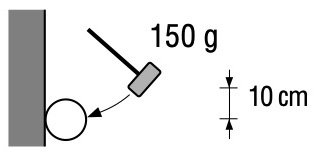
\includegraphics[scale=1]{K1.png}		& \SI{0,15}{\joule}	& 										& 								\\
02 				& 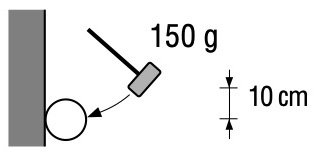
\includegraphics[scale=1]{K1.png}		& \SI{0,20}{\joule}	& 	AG1								& 1							\\
03 				& 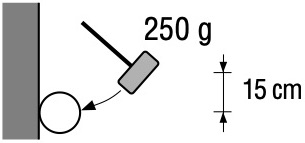
\includegraphics[scale=1]{K3.png}		& \SI{0,35}{\joule}	& 										& 								\\
04 				& 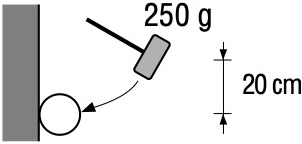
\includegraphics[scale=1]{K4.png}		& \SI{0,50}{\joule}	& 										& 3							\\
05 				& 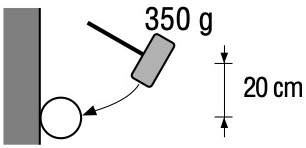
\includegraphics[scale=1]{K5.png}		& \SI{0,70}{\joule}	& 										& 								\\
06 				& 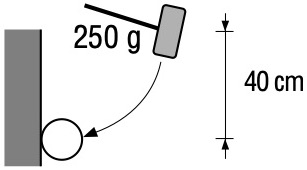
\includegraphics[scale=1]{K6.png}		& \SI{1}{\joule}		& 										& 								\\
07 				& 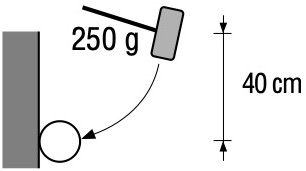
\includegraphics[scale=1]{K7.png}		& \SI{2}{\joule}		& 	AG2								& 5							\\
08 				& 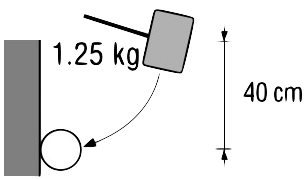
\includegraphics[scale=1]{K8.png}		& \SI{5}{\joule}		& 	AG3								& 								\\
08 				& 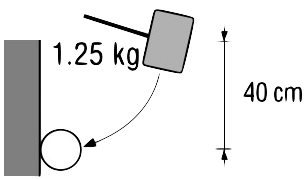
\includegraphics[scale=1]{K8.png}		& \SI{5}{\joule}		& 	AG3								& 								\\
09 				& 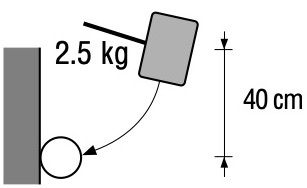
\includegraphics[scale=1]{K9.png}		& \SI{10}{\joule}		& 	AG3								& 								\\
10 				& 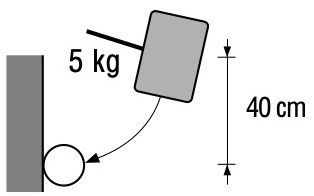
\includegraphics[scale=1]{K10.png}	& \SI{20}{\joule}		& 	AG4								& 								\\
\bottomrule
\end{tabularx}
\begin{tablenotes}
    \item[1] Corresponsdances avec le code AG de la classification des influences externes issu de la norme NF C 15-100.
\end{tablenotes}
\end{threeparttable} %note dans tableau
\end{table}
\end{minipage}
\hfill
\begin{minipage}[t]{0.39\linewidth}
\begin{table}[H]
\caption{Lettre additionnelle sur les informations supplémentaires}
\begin{tabularx}{\linewidth}{P{1.5cm} X}
\toprule
\thead{Lettre}		& \thead{Signification} \\
\midrule
f							& Résistant aux huiles \\
\addlinespace
H							& Appareil à haute tension \\
\addlinespace
M							& Appareil en déplacement durant le test à l'eau \\
\addlinespace
S							& Appareil immobile durant le test à l'eau \\
\addlinespace
W							& Conditions environnementales spécifiées \\
\bottomrule
\end{tabularx}
\end{table}
\end{minipage}

\newpage
\begin{landscape}
\newpage

%--------------------------------------
%ELECTROTECHNIQUE - SCHEMA DE LIAISON A LA TERRE
%--------------------------------------

%utiliser les environnement \begin{comment} \end{comment} pour mettre en commentaire le préambule une fois la programmation appelée dans le document maître (!ne pas oublier de mettre en commentaire \end{document}!)

\begin{comment}

\documentclass[a4paper, 11pt, twoside, fleqn]{memoir}

\usepackage{AOCDTF}

%--------------------------------------
%CANEVAS
%--------------------------------------

\newcommand\BoxColor{\ifcase\thechapshift blue!30\or brown!30\or pink!30\or cyan!30\or green!30\or teal!30\or purple!30\or red!30\or olive!30\or orange!30\or lime!30\or gray!\or magenta!30\else yellow!30\fi} %définition de la couleur des marqueurs de chapitre

\newcounter{chapshift} %compteur de chapitre du marqueur de chapitre
\addtocounter{chapshift}{-1}
	
\newif\ifFrame %instruction conditionnelle pour les couleurs des pages
\Frametrue

\pagestyle{plain}

% the main command; the mandatory argument sets the color of the vertical box
\newcommand\ChapFrame{%
\AddEverypageHook{%
\ifFrame
\ifthenelse{\isodd{\value{page}}}
  {\backgroundsetup{contents={%
  \begin{tikzpicture}[overlay,remember picture]
  \node[
  	rounded corners=3pt,
    fill=\BoxColor,
    inner sep=0pt,
    rectangle,
    text width=1.5cm,
    text height=5.5cm,
    align=center,
    anchor=north west
  ] 
  at ($ (current page.north west) + (-0cm,-2*\thechapshift cm) $) %nombre négatif = espacement des marqueurs entre les différents chapitres (à régler en fin de rédaction) (4.5cm vaut un espacement équivalement à la hauteur du marqueur, une page peut en contenir 6 avec cet espacement-la mais il est le plus équilibré)
    {\rotatebox{90}{\hspace*{.5cm}%
      \parbox[c][1.2cm][t]{5cm}{%
        \raggedright\textcolor{black}{\sffamily\textbf{\leftmark}}}}};
  \end{tikzpicture}}}
  }
  {\backgroundsetup{contents={%
  \begin{tikzpicture}[overlay,remember picture]
  \node[
  	rounded corners=3pt,
    fill=\BoxColor,
    inner sep=0pt,
    rectangle,
    text width=1.5cm,
    text height=5.5cm,
    align=center,
    anchor=north east
  ] 
  at ($ (current page.north east) + (-0cm,-2*\thechapshift cm) $) %nombre négatif = espacement des marqueurs entre les différents chapitres (à régler en fin de rédaction) (4.5cm vaut un espacement équivalement à la hauteur du marqueur, une page peut en contenir 6 avec cet espacement-la mais il est le plus équilibré)
    {\rotatebox{90}{\hspace*{.5cm}%
      \parbox[c][1.2cm][t]{5cm}{%
        \raggedright\textcolor{black}{\sffamily\textbf{\leftmark}}}}};
  \end{tikzpicture}}}%
  }
  \BgMaterial%
  \fi%
}%
  \stepcounter{chapshift}
}

\renewcommand\chaptermark[1]{\markboth{\thechapter.~#1}{}} %redéfinition du marqueur de chapitre pour ne contenir que le titre du chapitre %à personnaliser selon le nombre de chapitre dans le cours

%--------------------------------------
%corps du document
%--------------------------------------

\begin{document} %corps du document
	\openleft %début de chapitre à gauche

\end{comment}

\begin{xltabular}{\linewidth}{p{0.3cm} m{2cm} X p{0.3cm} m{2cm} X p{0.3cm} m{2.2cm} X}
\caption{Descriptif des indices de protection} 
\\
\toprule
\multicolumn{3}{c}{\thead{Protection contre les corps solides}}	& \multicolumn{3}{c}{\thead{Lettre additionnelle\\Contact direct avec les parties dangereuses}}	& \multicolumn{3}{c}{\thead{Protection contre les liquides}} \\
\midrule
\endfirsthead %en-tête de la première page du tableau  

\toprule
\multicolumn{3}{c}{\thead{Protection contre les corps solides}}	& \multicolumn{3}{c}{\thead{Lettre additionnelle\\Contact direct avec les parties dangereuses}}	& \multicolumn{3}{c}{\thead{Protection contre les liquides}} \\
\midrule
\endhead %en-tête de la première page du tableau  

\addlinespace
\midrule %filet de milieu de tableau
\multicolumn{9}{r}{\small\textit{Page suivante}}
\endfoot %pied de page de toutes les pages du tableau

\bottomrule
\endlastfoot %pied de page de la dernièredu tableau

0 		& 									& Aucune protection	&	&	&	& 0 	&	&	Aucune protection \\
1 		& 	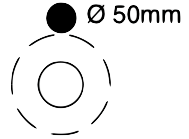
\includegraphics[scale=1.1]{1X.png} & Protégé contre les corps solides $\diameter \geq \SI{50}{\milli\meter}$  	&	A & 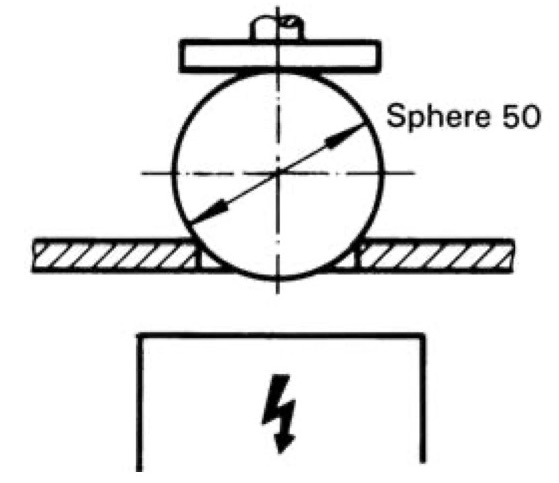
\includegraphics[width=2cm]{A.png}	&	Le dos de la main reste éloigné des parties dangereuses.	& 1 & 	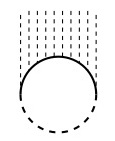
\includegraphics[scale=1.1]{X1.png}	&	Protégé contre les chutes verticales de gouttes d'eau (condensation) \\
2 		& 	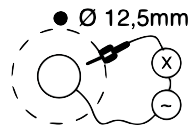
\includegraphics[scale=1.1]{2X.png} & Protégé contre les corps solides $\diameter \geq \SI{12,5}{\milli\meter}$  	& B	& 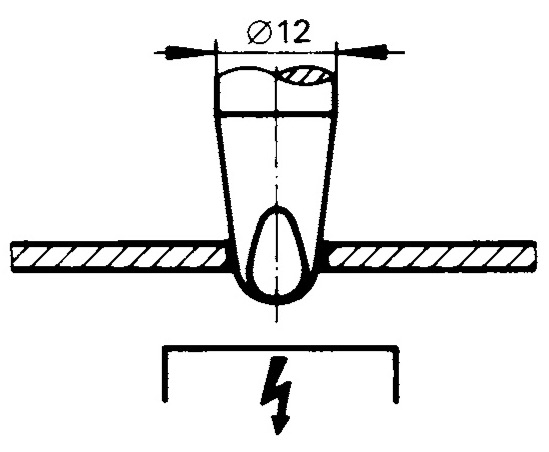
\includegraphics[width=2cm]{B.png}	&	L'introduction d'un doigt ne permet pas de toucher les parties dangereuses. & 2 & 	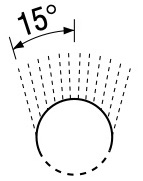
\includegraphics[scale=1.1]{X2.png}	&	Protégé contre les chutes de gouttes d'eau jusqu'à 15° de la verticale \\
3 		& 	
\includegraphics[scale=1.1]{3X.png} & Protégé contre les corps solides $\diameter \geq \SI{2,5}{\milli\meter}$  	& C	& 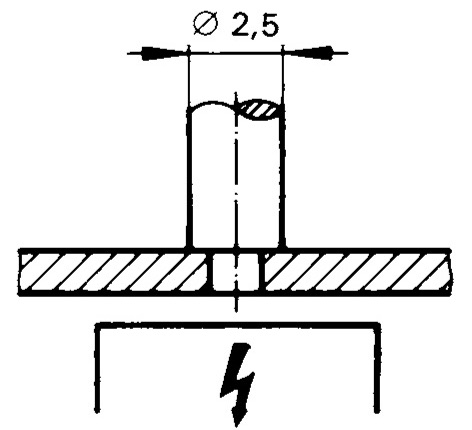
\includegraphics[width=2cm]{C.png}	&	L'introduction d'un outil ne permet pas de toucher les parties dangereuses. & 3 & 	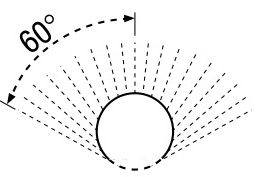
\includegraphics[scale=1.1]{X3.png}	&	Protégé contre l'eau de pluie jusqu'à 60° de la verticale \\
4 		& 	
\includegraphics[scale=1.1]{4X.png} & Protégé contre les corps solides $\diameter \geq \SI{1}{\milli\meter}$  	& D	& 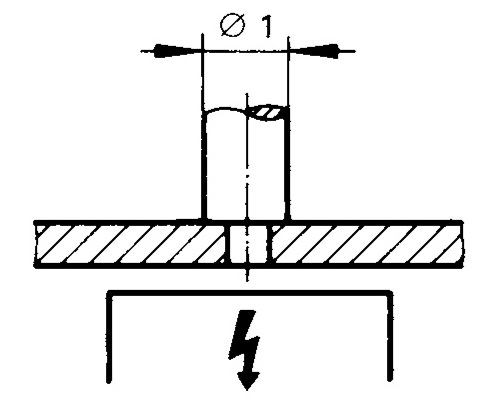
\includegraphics[width=2cm]{D.png}	&	L'introduction d'un outil fin ne permet pas de toucher les parties dangereuses. & 4 & 	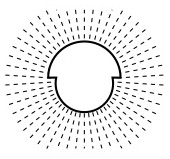
\includegraphics[scale=1.1]{X4.png}	&	Protégé contre les projections d'eau dans toutes les directions \\
5 		& 	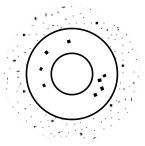
\includegraphics[scale=1.1]{5X.png} & Protégé contre la poussière (pas de dépot nuisible)  	& 	& & & 5 & 	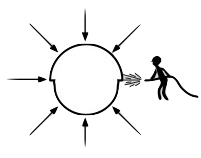
\includegraphics[scale=1.1]{X5.png}	&	Protégé contre les jets d'eau dans toutes les directions à la lance \\
6 		& 	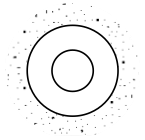
\includegraphics[scale=1.1]{6X.png} & Totalement protégé contre la poussière 	& 	& & & 6 & 	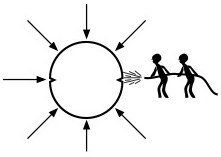
\includegraphics[scale=1.1]{X6.png}	&	Protégé contre les projections d'eau assimilables aux paquets de mer \\
 		&  & 	& 	& & & 7 & 	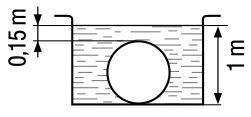
\includegraphics[scale=1.1]{X7.png}	&	Protégé contre les effets d'une immersion temporaire dans l'eau \\
		&  & 	& 	& & & 8 & 	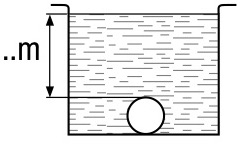
\includegraphics[scale=1.1]{X8.png}	&	Protégé contre les effets d'une immersion prolongée dans l'eau dans des conditions spécifiées \\
		&  & 	& 	& & & 9\tnote{1} & 	&	Protégé contre les jets d'eau haute pression et haute température mais pas nécessairement submersible \\
\end{xltabular}	


%\end{document}



\newpage
\end{landscape}
\newpage
\subsubsection{Classification des locaux selon l'IP}

Selon les locaux à équiper, leurs emplacements et les conditions particulières d'installation, la norme NF C 15-100 indique une protection minimale spécifiée par les indices IP et IK.

%--------------------------------------
%ELECTROTECHNIQUE - SCHEMA DE LIAISON A LA TERRE
%--------------------------------------

%utiliser les environnement \begin{comment} \end{comment} pour mettre en commentaire le préambule une fois la programmation appelée dans le document maître (!ne pas oublier de mettre en commentaire \end{document}!)

\begin{comment}

\documentclass[a4paper, 11pt, twoside, fleqn]{memoir}

\usepackage{AOCDTF}

%--------------------------------------
%CANEVAS
%--------------------------------------

\newcommand\BoxColor{\ifcase\thechapshift blue!30\or brown!30\or pink!30\or cyan!30\or green!30\or teal!30\or purple!30\or red!30\or olive!30\or orange!30\or lime!30\or gray!\or magenta!30\else yellow!30\fi} %définition de la couleur des marqueurs de chapitre

\newcounter{chapshift} %compteur de chapitre du marqueur de chapitre
\addtocounter{chapshift}{-1}
	
\newif\ifFrame %instruction conditionnelle pour les couleurs des pages
\Frametrue

\pagestyle{plain}

% the main command; the mandatory argument sets the color of the vertical box
\newcommand\ChapFrame{%
\AddEverypageHook{%
\ifFrame
\ifthenelse{\isodd{\value{page}}}
  {\backgroundsetup{contents={%
  \begin{tikzpicture}[overlay,remember picture]
  \node[
  	rounded corners=3pt,
    fill=\BoxColor,
    inner sep=0pt,
    rectangle,
    text width=1.5cm,
    text height=5.5cm,
    align=center,
    anchor=north west
  ] 
  at ($ (current page.north west) + (-0cm,-2*\thechapshift cm) $) %nombre négatif = espacement des marqueurs entre les différents chapitres (à régler en fin de rédaction) (4.5cm vaut un espacement équivalement à la hauteur du marqueur, une page peut en contenir 6 avec cet espacement-la mais il est le plus équilibré)
    {\rotatebox{90}{\hspace*{.5cm}%
      \parbox[c][1.2cm][t]{5cm}{%
        \raggedright\textcolor{black}{\sffamily\textbf{\leftmark}}}}};
  \end{tikzpicture}}}
  }
  {\backgroundsetup{contents={%
  \begin{tikzpicture}[overlay,remember picture]
  \node[
  	rounded corners=3pt,
    fill=\BoxColor,
    inner sep=0pt,
    rectangle,
    text width=1.5cm,
    text height=5.5cm,
    align=center,
    anchor=north east
  ] 
  at ($ (current page.north east) + (-0cm,-2*\thechapshift cm) $) %nombre négatif = espacement des marqueurs entre les différents chapitres (à régler en fin de rédaction) (4.5cm vaut un espacement équivalement à la hauteur du marqueur, une page peut en contenir 6 avec cet espacement-la mais il est le plus équilibré)
    {\rotatebox{90}{\hspace*{.5cm}%
      \parbox[c][1.2cm][t]{5cm}{%
        \raggedright\textcolor{black}{\sffamily\textbf{\leftmark}}}}};
  \end{tikzpicture}}}%
  }
  \BgMaterial%
  \fi%
}%
  \stepcounter{chapshift}
}

\renewcommand\chaptermark[1]{\markboth{\thechapter.~#1}{}} %redéfinition du marqueur de chapitre pour ne contenir que le titre du chapitre %à personnaliser selon le nombre de chapitre dans le cours

%--------------------------------------
%corps du document
%--------------------------------------

\begin{document} %corps du document
	\openleft %début de chapitre à gauche

\end{comment}

\captionof{table}{Classification des locaux}
\vspace{-1em}
\begin{minipage}[t]{0.49\linewidth}
\begin{tabularx}{\textwidth}[t]{c X c c}
\toprule
\multicolumn{2}{c}{\thead{Type de\\local}}																				& \thead{IP}	& \thead{IK}  \\
\midrule
\multicolumn{4}{p{0.95\textwidth}}{\textit{Locaux (ou emplacements) domestiques et analogues}} \\
\middashrule \\
\multicolumn{2}{p{4.8cm}}{Auvents}																							& 24				& 07 \\
\multicolumn{2}{p{4.8cm}}{Bains (salle de)}																				& \multicolumn{2}{p{2.2cm}}{(voir salles d'eau)} \\
\multicolumn{2}{p{4.8cm}}{Bicyclettes, cyclomoteurs, voitures pour enfants (locaux pour)}			& 20				& 07 \\
\multicolumn{2}{p{4.8cm}}{Branchement eau, égout, chauffage}												& 23				& 02 \\
\multicolumn{2}{p{4.8cm}}{Buanderies}																					& 23				& 02 \\
\multicolumn{2}{p{4.8cm}}{Caves, celliers, garage, local avec chaudière}									& 20				& 02--07 \\
\multicolumn{2}{p{4.8cm}}{Chambres	}																					& 20				& 02 \\
\multicolumn{2}{p{4.8cm}}{Collecte des ordures (locaux pour)}												& 25				& 07 \\
\multicolumn{2}{p{4.8cm}}{Couloirs de cave}																			& 20				& 07 \\
\multicolumn{2}{p{4.8cm}}{Cours}																							& 24--25			& 02--07 \\
\multicolumn{2}{p{4.8cm}}{Cuisines}																						& 20				& 02 \\
\multicolumn{2}{p{4.8cm}}{Douches}																						& \multicolumn{2}{p{2.2cm}}{(voir salles d'eau)} \\
\multicolumn{2}{p{4.8cm}}{Escaliers intérieurs, coursives intérieures}										& 20				& 02--07 \\
\multicolumn{2}{p{4.8cm}}{Escaliers extérieures, coursives extérieures non couvertes}				& 24				& 07 \\
\multicolumn{2}{p{4.8cm}}{Coursives extérieures couvertes}														& 21				& 02 \\
\multicolumn{2}{p{4.8cm}}{Greniers (combles)}																			& 20				& 02 \\
\multicolumn{2}{p{4.8cm}}{Abris de jardins	}																			& 24--25			& 02--07 \\
\multicolumn{2}{p{4.8cm}}{Lieux d'aisances}																			& 20				& 02 \\
\multicolumn{2}{p{4.8cm}}{Locaux à poubelles}																		& 25				& 02--07 \\
\multicolumn{2}{p{4.8cm}}{Lingeries, salles de repassage}														& 21				& 02 \\
\multicolumn{2}{p{4.8cm}}{Rampes d'accès au garage}																& 25				& 07 \\
\multicolumn{2}{p{4.8cm}}{Salles d'eau, locaux contenant une baignoire ou une douche :	}		& 					& \\
& volume 0																& 27				& 02 \\
& volume 1																& 24				& 02 \\
& volume 2																& 23				& 02 \\
& volume 3																& 21				& 02 \\
\multicolumn{2}{p{4.8cm}}{Salles de séjour}																				& 20				& 02 \\
\multicolumn{2}{p{4.8cm}}{Séchoirs}																						& 21				& 02 \\
\end{tabularx}
\end{minipage}
\hfill
\begin{minipage}[t]{0.49\linewidth}
\begin{tabularx}{\textwidth}[t]{c X c c}
\toprule
\multicolumn{2}{c}{\thead{Type de\\local}}																				& \thead{IP}	& \thead{IK}  \\
\midrule
\multicolumn{4}{p{0.95\textwidth}}{\textit{Locaux (ou emplacements) domestiques et analogues}} \\
\middashrule \\
\multicolumn{2}{p{4.8cm}}{Sous-sols}																						& 21				& 02/07 \\
\multicolumn{2}{p{4.8cm}}{Terrasses couvertes}																		& 21				& 02 \\
\multicolumn{2}{p{4.8cm}}{Toilettes (cabinets de)}																	& 21				& 02 \\
\multicolumn{2}{p{4.8cm}}{Vérandas}																						& 21				& 02 \\
\multicolumn{2}{p{4.8cm}}{Vides sanitaires}																				& 23				& 02--07 \\
\addlinespace
\midrule
\multicolumn{4}{p{0.95\textwidth}}{\textit{Locaux techniques}} \\
\middashrule \\
\multicolumn{2}{p{4.8cm}}{Accumulateurs (salles d')}																& 23				& 02--07 \\
\multicolumn{2}{p{4.8cm}}{Ascenseurs (locaux des machines et locaux des poulies)}					& 20				& 07--08 \\	
\multicolumn{2}{p{4.8cm}}{Service électrique}																			& 20				& 07 \\
\multicolumn{2}{p{4.8cm}}{Salles des commandes}																	& 20				& 02 \\
\multicolumn{2}{p{4.8cm}}{Ateliers}																							& 21--23			& 07--08 \\
\multicolumn{2}{p{4.8cm}}{Laboratoires}																					& 21--23			& 02--07 \\
\multicolumn{2}{p{4.8cm}}{Laveurs de conditionnement d'air	}													& 24				& 07 \\
\multicolumn{2}{p{4.8cm}}{Garages (servant exclusivement au stationnement des véhicules) d'une surface n'excédant pas \SI{100}{\square\meter}}	& 21				& 07 \\
\multicolumn{2}{p{4.8cm}}{Laveurs de conditionnement d'air}													& 24				& 07 \\
\multicolumn{2}{p{4.8cm}}{Machines (salles de)}																		& 31				& 07--08 \\
\multicolumn{2}{p{4.8cm}}{Surpresseurs d'eau}																		& 23				& 07--08 \\
\multicolumn{2}{p{4.8cm}}{Chaufferies et locaux annexes :}														& 					& \\
&	 à charbon																																& 51--61			& 07--08 \\
&	 autres combustibles																												& 21				& 07--08 \\
&	 électriques																															& 21				& 07--08 \\
\addlinespace
\midrule
\multicolumn{4}{p{0.95\textwidth}}{\textit{Garages et parcs de stationnement couverts d'une surface supérieure à \SI{100}{\square\meter}}} \\
\middashrule \\
\multicolumn{2}{p{4.8cm}}{Aires de stationnement}																	& 21				& 07--20 \\
\multicolumn{2}{p{4.8cm}}{Zones de lavage (à l'intérieur du local)}											& 25				& 07 \\
\multicolumn{2}{p{4.8cm}}{Zones de sécurité :}																		& 					&  \\
	&	à l'intérieur																														& 21				& 07 \\
	&	à l'extérieur																														& 24				& 07 \\
\multicolumn{2}{p{4.8cm}}{Zones de graissage}																			& 23				& 08 \\

\end{tabularx}
\end{minipage}
\begin{minipage}{0.49\textwidth}
\begin{tabularx}{\textwidth}{R}
\midrule
\small\textit{Colonne suivante} \\
\end{tabularx}
\end{minipage}
\hfill
\begin{minipage}{0.49\textwidth}
\begin{tabularx}{\textwidth}{R}
\midrule
\small\textit{Page suivante} \\
\end{tabularx}
\end{minipage}
\begin{minipage}[t]{0.49\linewidth}
\begin{tabularx}{\textwidth}[t]{c X c c}
\multicolumn{4}{l}{\small\textit{Page précédente}} \\
\midrule
\multicolumn{2}{c}{\thead{Type de\\local}}																				& \thead{IP}	& \thead{IK}  \\
\midrule
\multicolumn{4}{p{0.95\textwidth}}{\textit{Garages et parcs de stationnement couverts d'une surface supérieure à \SI{100}{\square\meter}}} \\
\middashrule \\
\multicolumn{2}{p{4.8cm}}{Locaux de recharge de batteries}															& 23				& 07 \\
\multicolumn{2}{p{4.8cm}}{Ateliers}																								& 21				& 08 \\
\addlinespace
\midrule
\multicolumn{4}{p{0.95\textwidth}}{\textit{Locaux sanitaires à usage collectif}} \\
\middashrule \\
\multicolumn{2}{p{4.8cm}}{Salles de lavabos individuels}																& 21				& 07 \\
\multicolumn{2}{p{4.8cm}}{Salles de WC à cuvettes (à l'anglaise)}													& 21				& 07 \\
\multicolumn{2}{p{4.8cm}}{Salles d'urinoirs}																					& 21				& 07 \\
\multicolumn{2}{p{4.8cm}}{Salles de lavabos collectifs}																	& 23				& 07 \\
\multicolumn{2}{p{4.8cm}}{Salles de WC à la turques, de douches à cabines individuelles, de douches collectives}								& 23				& 07 \\
\multicolumn{2}{p{4.8cm}}{Buanderies collectives}																		& 24				& 07 \\
\addlinespace
\midrule
\multicolumn{4}{p{0.95\textwidth}}{\textit{Bâtiments à usage collectif (autre que ERP)}} \\
\middashrule \\
\multicolumn{2}{p{4.8cm}}{Bureaux}																							& 20				& 02 \\
\multicolumn{2}{p{4.8cm}}{Bibliothèques}																					& 20				& 02 \\
\multicolumn{2}{p{4.8cm}}{Salles d'archives}																				& 20				& 02 \\
\multicolumn{2}{p{4.8cm}}{Salles d'informatiques}																		& 20				& 02 \\
\multicolumn{2}{p{4.8cm}}{Salles de dessin}																					& 20				& 02 \\
\multicolumn{2}{p{4.8cm}}{Locaux regroupant les machines de reproduction de plans et de documents}			& 20				& 02 \\
\multicolumn{2}{p{4.8cm}}{Salles de tri}																						& 20				& 07 \\
\multicolumn{2}{p{4.8cm}}{Salles de restaurant et de cantine, grandes cuisines}							& 21				& 07 \\
\multicolumn{2}{p{4.8cm}}{Salles de sports}																					& 21				& 07--08 \\
\multicolumn{2}{p{4.8cm}}{Locaux de casernement}																		& 21				& 07 \\
\multicolumn{2}{p{4.8cm}}{Salles de réunion}																				& 20				& 02 \\
\multicolumn{2}{p{4.8cm}}{Salles d'attentes, salons, hall}																& 20				& 02 \\
\multicolumn{2}{p{4.8cm}}{Salles de consultation à usage médical, ne comportant pas d'équipements spécifiques}		& 20				& 02 \\
\multicolumn{2}{p{4.8cm}}{Salles de démonstration et d'exposition}												& 20				& 02 \\
\addlinespace
\midrule
\multicolumn{4}{p{0.95\textwidth}}{\textit{Locaux (ou emplacements) dans les exploitations agricoles}} \\
\middashrule \\
\multicolumn{2}{p{4.8cm}}{Alcools (entrepôts de)}																		& 23				& 07 \\
\end{tabularx}
\end{minipage}
\hfill
\begin{minipage}[t]{0.49\linewidth}
\begin{tabularx}{\textwidth}[t]{c X c c}
\multicolumn{4}{l}{\small\textit{Colonne précédente}} \\
\midrule
\multicolumn{2}{c}{\thead{Type de\\local}}																				& \thead{IP}	& \thead{IK}  \\
\midrule
\multicolumn{4}{p{0.95\textwidth}}{\textit{Locaux (ou emplacements) dans les exploitations agricoles}} \\
\middashrule \\
\multicolumn{2}{p{4.8cm}}{Bergeries fermées}																				& 35				& 07 \\
\multicolumn{2}{p{4.8cm}}{Buanderies}																					& 24				& 07 \\
\multicolumn{2}{p{4.8cm}}{Battages de céréales}																		& 50				& 07 \\
\multicolumn{2}{p{4.8cm}}{Bûchers}																							& 30				& 10 \\
\multicolumn{2}{p{4.8cm}}{Caves de distillation}																		& 23				& 07 \\
\multicolumn{2}{p{4.8cm}}{Chais (vin)	}																					& 23				& 07 \\
\multicolumn{2}{p{4.8cm}}{Cours}																							& 35				& 07 \\
\multicolumn{2}{p{4.8cm}}{\'Elevages de volailles}																	& 35				& 07 \\
\multicolumn{2}{p{4.8cm}}{\'Ecuries}																						& 35				& 07 \\
\multicolumn{2}{p{4.8cm}}{Engrais (dépôts d')}																			& 50				& 07 \\
\multicolumn{2}{p{4.8cm}}{\'Etables}																						& 35				& 07 \\
\multicolumn{2}{p{4.8cm}}{Fumières}																						& 24				& 07 \\
\multicolumn{2}{p{4.8cm}}{Fenils}																							& 50				& 07 \\
\multicolumn{2}{p{4.8cm}}{Fourrage (entrepôts de)}																	& 50				& 07 \\
\multicolumn{2}{p{4.8cm}}{Greniers, granges}																			& 50				& 07 \\
\multicolumn{2}{p{4.8cm}}{Paille (entrepôts de)}																		& 50				& 07 \\
\multicolumn{2}{p{4.8cm}}{Serres}																							& 23				& 07 \\
\multicolumn{2}{p{4.8cm}}{Silos à céréales}																				& 50				& 07 \\
\multicolumn{2}{p{4.8cm}}{Traies (salle de)}																				& 35				& 07 \\
\multicolumn{2}{p{4.8cm}}{Porcheries}																						& 35				& 07 \\
\multicolumn{2}{p{4.8cm}}{Poulaillers}																						& 35				& 07 \\
\addlinespace
\midrule
\multicolumn{4}{p{0.95\textwidth}}{\textit{Installations diverses}} \\
\middashrule \\
\multicolumn{2}{p{4.8cm}}{Terrains de camping et caravaning}													& 34				& 07 \\
\multicolumn{2}{p{4.8cm}}{Quais de ports de plaisance}															& 34				& 08 \\
\multicolumn{2}{p{4.8cm}}{Chantiers}																						& 44				& 08 \\
\multicolumn{2}{p{4.8cm}}{Quais de chargement}																		& 35				& 08 \\
\multicolumn{2}{p{4.8cm}}{Rues, cours, jardins et autres emplacements extérieurs}					& 34--35			& 07 \\
\multicolumn{2}{p{4.8cm}}{\'Etablissement forains}																	& 33				& 08 \\
\multicolumn{2}{p{4.8cm}}{Piscines :}																						& 					&	  \\
& volume 0																																& 28				& 02 \\
& volume 1																																& 25				& 02 \\
& volume 2																																& 22--24			& 02 \\
\multicolumn{2}{p{4.8cm}}{Saunas}																							& 34				& 02 \\
\multicolumn{2}{p{4.8cm}}{Bassins de fontaines}																		& 37				& 02 \\
\multicolumn{2}{p{4.8cm}}{Traitements des eaux (local de)}														& 24--25			& 07--08 \\
\addlinespace
\midrule
\multicolumn{4}{p{0.95\textwidth}}{\textit{Installations thermodynamiques, chambres climatisées et chambres froides}} \\
\middashrule \\
\end{tabularx}
\end{minipage}
\begin{minipage}[b]{0.49\textwidth}
\begin{xltabular}{\textwidth}{R}
\midrule
\small\textit{Colonne suivante} \\
\end{xltabular}
\end{minipage}
\hfill
\begin{minipage}[b]{0.49\textwidth}
\begin{xltabular}{\textwidth}{R}
\midrule
\small\textit{Page suivante} \\
\end{xltabular}
\end{minipage}
\begin{minipage}[t]{0.49\linewidth}
\begin{tabularx}{\textwidth}[t]{c X c c}
\multicolumn{4}{l}{\small\textit{Page précédente}} \\
\midrule
\multicolumn{2}{c}{\thead{Type de\\local}}																				& \thead{IP}	& \thead{IK}  \\
\midrule
\multicolumn{4}{p{0.95\textwidth}}{\textit{Installations thermodynamiques, chambres climatisées et chambres froides}} \\
\middashrule \\
\multicolumn{2}{p{4.8cm}}{Température < \SI{-10}{\celsius}}												&	23				&	07 \\	
\multicolumn{2}{p{4.8cm}}{Hauteur au dessus du sol :}															& 					&  \\
& \SIrange[range-phrase=\ à\ ]{0}{1,10}{\meter}																		& 24				& 07 \\
& \SIrange[range-phrase=\ à\ ]{1,10}{2}{\meter}																		& 21				& 07 \\
& au-dessus de \SI{2}{\meter}																									& 21				& 07 \\
& sous l'évaporateur ou tube																									& 21				& 07 \\
& écoulement d'eau																													& 21				& 07 \\
\multicolumn{2}{p{4.8cm}}{Plafond et jusqu'à \SI{10}{\centi\meter} en-dessous}	 				&	23				&	07 \\	
\multicolumn{2}{p{4.8cm}}{Compresseur :}																			& 					&  \\
& local																																		& 21				& 08 \\
& monobloc placé à l'extérieur ou en terrasse																				& 34				& 08 \\
\midrule
\multicolumn{4}{p{0.95\textwidth}}{\textit{\'Etablissements industriels}} \\
\middashrule \\
\multicolumn{2}{p{4.8cm}}{Abattoirs}																	 				&	55				&	08 \\	
\multicolumn{2}{p{4.8cm}}{Accumulateurs (fabrication d')}										 				&	33				&	07 \\	
\multicolumn{2}{p{4.8cm}}{Acide (fabrication et dépôts)}										 				&	33				&	07 \\	
\multicolumn{2}{p{4.8cm}}{Alcool (fabrication et dépôts)}										 				&	33				&	07 \\	
\multicolumn{2}{p{4.8cm}}{Aluminium (fabrication et dépôts)}										 		&	51--53		&	08 \\	
\multicolumn{2}{p{4.8cm}}{Animaux (élevage et engraissement)}										 	&	45				&	07 \\	
\multicolumn{2}{p{4.8cm}}{Asphaltes, bitume (dépôts d')}										 				&	53				&	07 \\	
\multicolumn{2}{p{4.8cm}}{Battage et cardage des laines}											 				&	50				&	08 \\	
\multicolumn{2}{p{4.8cm}}{Blanchisseries}																 				&	23--24		&	07 \\	
\multicolumn{2}{p{4.8cm}}{Bois (travail du)}																 			&	50				&	08 \\
\multicolumn{2}{p{4.8cm}}{Boucheries}																		 			&	24--25		&	07 \\	
\multicolumn{2}{p{4.8cm}}{Boucheries}																		 			&	24--25		&	07 \\	
\multicolumn{2}{p{4.8cm}}{Brasseries}																		 			&	24				&	07 \\	
\multicolumn{2}{p{4.8cm}}{Briqueteries}																		 		&	53--54		&	08 \\	
\multicolumn{2}{p{4.8cm}}{Caoutchouc (fabrication et transformation)}								 	&	54				&	07 \\	
\multicolumn{2}{p{4.8cm}}{Carbure (fabrication et dépôts)}								 					&	51				&	07 \\	
\multicolumn{2}{p{4.8cm}}{Cartoucherie}								 												&	53				&	08 \\	
\multicolumn{2}{p{4.8cm}}{Cartons (fabrication de}																&	33				&	07 \\	
\multicolumn{2}{p{4.8cm}}{Carrières}									 												&	55				&	08 \\
\multicolumn{2}{p{4.8cm}}{Celluloïd (fabrication d'objets}														&	30				&	08 \\	
\multicolumn{2}{p{4.8cm}}{Cellulose (fabrication)}									 								&	34				&	08 \\	
\end{tabularx}
\end{minipage}
\hfill
\begin{minipage}[t]{0.49\linewidth}
\begin{tabularx}{\textwidth}[t]{c X c c}
\multicolumn{4}{l}{\small\textit{Colonne précédente}} \\
\midrule
\multicolumn{2}{c}{\thead{Type de\\local}}																				& \thead{IP}	& \thead{IK}  \\
\midrule
\multicolumn{4}{p{0.95\textwidth}}{\textit{\'Etablissements industriels}} \\
\middashrule \\
\multicolumn{2}{p{4.8cm}}{Charbon (entrepôts de)}									 							&	54				&	08 \\	
\multicolumn{2}{p{4.8cm}}{Charcuteries}									 											&	24				&	07 \\	
\multicolumn{2}{p{4.8cm}}{Chaudronneries}									 										&	30				&	08 \\	
\multicolumn{2}{p{4.8cm}}{Chaux (fours à)}									 										&	50				&	08 \\	
\multicolumn{2}{p{4.8cm}}{Chiffons (entrepôts de)}									 							&	30				&	07 \\	
\multicolumn{2}{p{4.8cm}}{Chlore (fabrication et dépôts)}									 					&	33				&	07 \\	
\multicolumn{2}{p{4.8cm}}{Chromage}									 												&	33				&	07 \\	
\multicolumn{2}{p{4.8cm}}{Cimenterie}									 												&	50				&	08 \\	
\multicolumn{2}{p{4.8cm}}{Cokerie}									 													&	53				&	08 \\	
\multicolumn{2}{p{4.8cm}}{Colle (fabrication de)}									 								&	33				&	07 \\
\multicolumn{2}{p{4.8cm}}{Chaines d'embouteillage}									 							&	35				&	08 \\	
\multicolumn{2}{p{4.8cm}}{Combustibles liquides (dépôts de)}												&	31--33		&	08 \\	
\multicolumn{2}{p{4.8cm}}{Corps gras (traitement de)}									 						&	51				&	07 \\	
\multicolumn{2}{p{4.8cm}}{Cuir (fabrication et dépôts de)}									 					&	31				&	08 \\	
\multicolumn{2}{p{4.8cm}}{Cuivre (traitement des minéraux)}									 				&	31				&	08 \\	
\multicolumn{2}{p{4.8cm}}{Décapage}									 												&	54				&	08 \\	
\multicolumn{2}{p{4.8cm}}{Détersifs (fabrication de produits)}									 			&	53				&	07 \\	
\multicolumn{2}{p{4.8cm}}{Distillerie}									 												&	33				&	07 \\	
\multicolumn{2}{p{4.8cm}}{\'Electrolyse}									 											&	03				&	08 \\	
\multicolumn{2}{p{4.8cm}}{Encre (fabrication d')}									 								&	31				&	07 \\	
\multicolumn{2}{p{4.8cm}}{Engrais (fabrication et dépôts de)}				 								&	53				&	07 \\	
\multicolumn{2}{p{4.8cm}}{Explosifs (fabrication et dépôts de)}				 								&	55				&	08 \\	
\multicolumn{2}{p{4.8cm}}{Fer (fabrication et traitement de)}				 									&	51				&	08 \\	
\multicolumn{2}{p{4.8cm}}{Filatures}									 													&	50			&	07 \\	
\multicolumn{2}{p{4.8cm}}{Fourrures (battage)}									 									&	50			&	07 \\	
\multicolumn{2}{p{4.8cm}}{Fromageries}									 											&	25			&	07 \\	
\multicolumn{2}{p{4.8cm}}{Gaz (usines et depôts de)}									 						&	31			&	08 \\	
\multicolumn{2}{p{4.8cm}}{Goudron (traitement de)}									 							&	33			&	07 \\	
\multicolumn{2}{p{4.8cm}}{Graineteries}									 											&	50			&	07 \\	
\multicolumn{2}{p{4.8cm}}{Gravures de métaux}																	&	33			&	07 \\	
\multicolumn{2}{p{4.8cm}}{Huile (extraction de)}																	&	31			&	07 \\	
\multicolumn{2}{p{4.8cm}}{Hydrocarbures (fabrication de)}														&	33--34	&	08 \\	
\multicolumn{2}{p{4.8cm}}{Imprimeries}																				&	20			&	08 \\	
\multicolumn{2}{p{4.8cm}}{Laiteries}																						&	25			&	07 \\	
\multicolumn{2}{p{4.8cm}}{Laveries, lavoirs publics}																&	25			&	07 \\	
\multicolumn{2}{p{4.8cm}}{Liqueurs (fabrication de)}																&	21			&	07 \\	
\end{tabularx}
\end{minipage}
\begin{minipage}[b]{0.49\textwidth}
\begin{xltabular}{\textwidth}{R}
\midrule
\small\textit{Colonne suivante} \\
\end{xltabular}
\end{minipage}
\hfill
\begin{minipage}[b]{0.49\textwidth}
\begin{xltabular}{\textwidth}{R}
\midrule
\small\textit{Page suivante} \\
\end{xltabular}
\end{minipage}
\begin{minipage}[t]{0.49\linewidth}
\begin{tabularx}{\textwidth}[t]{c X c c}
\multicolumn{4}{l}{\small\textit{Page précédente}} \\
\midrule
\multicolumn{2}{c}{\thead{Type de\\local}}																				& \thead{IP}	& \thead{IK}  \\
\midrule
\multicolumn{4}{p{0.95\textwidth}}{\textit{\'Etablissements industriels}} \\
\middashrule \\
\multicolumn{2}{p{4.8cm}}{Liquides halogénés (emploi de)}													&	21			&	08 \\	
\multicolumn{2}{p{4.8cm}}{Liquides inflammables (dépôts, ateliers ou l'on emploie des)}			&	21			&	08 \\	
\multicolumn{2}{p{4.8cm}}{Magnésium (fabrication, travail et depôts de)}								&	31			&	07 \\	
\multicolumn{2}{p{4.8cm}}{Machines (salle des)}																	&	20			&	08 \\	
\multicolumn{2}{p{4.8cm}}{Matières plastiques (fabrication de)}												&	51			&	08 \\	
\multicolumn{2}{p{4.8cm}}{Menuiseries}																				&	50			&	08 \\	
\multicolumn{2}{p{4.8cm}}{Métaux (traitement de)}									 							&	31--33	&	08 \\	
\multicolumn{2}{p{4.8cm}}{Moteurs thermiques (essai de)}									 					&	30			&	08 \\	
\multicolumn{2}{p{4.8cm}}{Munitions (dépôts de)}									 								&	33			&	08 \\	
\multicolumn{2}{p{4.8cm}}{Nickel (traitement des minérais)}									 				&	33			&	08 \\	
\multicolumn{2}{p{4.8cm}}{Ordures ménagères (traitement d')}								 				&	53--54	&	07 \\	
\multicolumn{2}{p{4.8cm}}{Papiers (fabriques de)}													 				&	33--34	&	07 \\	
\multicolumn{2}{p{4.8cm}}{Papiers (dépôts de)}													 					&	31			&	07 \\	
\multicolumn{2}{p{4.8cm}}{Parfum (fabrication et dépôts de)}													&	31			&	07 \\	
\multicolumn{2}{p{4.8cm}}{Pâte à papiers (préparation de)}													&	34			&	07 \\	
\multicolumn{2}{p{4.8cm}}{Peinture (fabrication et dépôts de)}												&	33			&	08 \\	
\multicolumn{2}{p{4.8cm}}{Plâtre (broyage et dépôts de)}														&	50			&	07 \\	
\multicolumn{2}{p{4.8cm}}{Poudreries}																					&	55			&	07 \\	
\multicolumn{2}{p{4.8cm}}{Produits chimiques (fabrication de)}												&	30--50	&	08 \\	
\multicolumn{2}{p{4.8cm}}{Raffinerie de pétrole}																	&	34			&	07 \\	
\multicolumn{2}{p{4.8cm}}{Salaisons}																					&	33			&	07 \\	
\multicolumn{2}{p{4.8cm}}{Savons (fabrication de)}																&	31			&	07 \\	
\multicolumn{2}{p{4.8cm}}{Scieries}																						&	50			&	08 \\	
\multicolumn{2}{p{4.8cm}}{Serrureries}																					&	30			&	08 \\	
\multicolumn{2}{p{4.8cm}}{Silos à céréales ou à sucre}															&	50			&	07 \\	
\multicolumn{2}{p{4.8cm}}{Soies et crins (préparation de)}														&	50			&	08 \\	
\multicolumn{2}{p{4.8cm}}{Soude (fabrication et dépôts de)}													&	33			&	07 \\	
\multicolumn{2}{p{4.8cm}}{Soude (traitement de)}																		&	51			&	07 \\	
\multicolumn{2}{p{4.8cm}}{Spiritueux (entrepôts de)}																&	33			&	07 \\	
\multicolumn{2}{p{4.8cm}}{Sucreries}																					&	55			&	07 \\	
\multicolumn{2}{p{4.8cm}}{Tanneries}																					&	35			&	07 \\	
\end{tabularx}
\end{minipage}
\hfill
\begin{minipage}[t]{0.49\linewidth}
\begin{tabularx}{\textwidth}[t]{c X c c}
\multicolumn{4}{l}{\small\textit{Colonne précédente}} \\
\midrule
\multicolumn{2}{c}{\thead{Type de\\local}}																				& \thead{IP}	& \thead{IK}  \\
\midrule
\multicolumn{4}{p{0.95\textwidth}}{\textit{\'Etablissements industriels}} \\
\middashrule \\
\multicolumn{2}{p{4.8cm}}{Teintureries}																				&	35			&	07 \\	
\multicolumn{2}{p{4.8cm}}{Textiles et tissus (fabrication de)}													&	51			&	08 \\	
\multicolumn{2}{p{4.8cm}}{Vernis (fabrication et application de)}											&	33			&	08 \\	
\multicolumn{2}{p{4.8cm}}{Verreries}																					&	33			&	08 \\	
\multicolumn{2}{p{4.8cm}}{Zinc (travail du)}																			&	31			&	08 \\	
\midrule
\multicolumn{4}{p{0.95\textwidth}}{\textit{\'Etablissements recevant du public (ERP)}} \\
\middashrule \\
L 	& \multicolumn{3}{p{0.75\textwidth}}{Salles d'audition, de conférence, de réunion, de spectacles ou à usages multiples :} \\
& salles																																	& 20			& 02--07 \\
& cages de scènes																													& 20			& 08 \\
& magasin de décors																												& 20			& 08 \\
& locaux des perruquiers et des cordonniers																			& 20			& 07 \\
M 	& \multicolumn{3}{p{0.8\textwidth}}{Magasins de vente, centres commerciaux :} \\
& locaux de ventes																												& 20			& 08 \\
& stockages et manipulations de matériels d'emballages															& 20			& 08 \\
N	& Restaurants et débits de boissons																					& 20			& 02 \\
O	& Hôtels et pensions de familles																							& 20			& 02 \\
P	& Salles de danse et salles de jeux																						& 20			& 07 \\
R 	& \multicolumn{3}{p{0.75\textwidth}}{\'Etablissements d'enseignement, colonies de vacances :} \\
& salles	 d'enseignement																										& 20			& 02 \\
& dortoirs																																& 20			& 07 \\
S	&  Bibliothèques, centres de documentation																		& 20			& 02 \\
T 	& \multicolumn{3}{p{0.75\textwidth}}{Expositions :} \\
& halls et salles																														& 21			& 07 \\
& locaux de réceptions de matériels et de marchandises															& 20			& 08 \\
U 	& \multicolumn{3}{p{0.75\textwidth}}{\'Etablissements sanitaires :} \\
& chambres																															& 20			& 02 \\
& incinérations																														& 21			& 07--08 \\
& blocs opératoires																												& 20			& 07 \\
\end{tabularx}
\end{minipage}
\begin{minipage}[b]{0.49\textwidth}
\begin{xltabular}{\textwidth}{R}
\midrule
\small\textit{Colonne suivante} \\
\end{xltabular}
\end{minipage}
\hfill
\begin{minipage}[b]{0.49\textwidth}
\begin{xltabular}{\textwidth}{R}
\midrule
\small\textit{Page suivante} \\
\end{xltabular}
\end{minipage}
\begin{minipage}[t]{0.49\linewidth}
%\begin{threeparttable}
\begin{tabularx}{\textwidth}[t]{c X c c}
\multicolumn{4}{l}{\small\textit{Page précédente}} \\
\midrule
\multicolumn{2}{c}{\thead{Type de\\local}}																				& \thead{IP}	& \thead{IK}  \\
\midrule
\multicolumn{4}{p{0.95\textwidth}}{\textit{\'Etablissements recevant du public (ERP)}} \\
\middashrule \\
U 	& \multicolumn{3}{p{0.75\textwidth}}{\'Etablissements sanitaires :} \\
& stérilisations centralisées																									& 24--25		& 02--07 \\
& pharmacies et laboratoires avec plus de \SI{10}{\liter} de liquides inflammatoires				& 21--23		& 02--07 \\
V & \'Etablissement de cultes 																									& 20				& 02 \\
W & Administrations et banques																								& 20				& 02 \\
X 	& \multicolumn{3}{p{0.75\textwidth}}{\'Etablissements sportifs couverts :} \\
& Salles																																	& 21				& 07--08 \\
& Locaux contenant des installations frigorifiques																	& 21				& 08 \\
Y & Musées																															& 20				& 02 \\
PA & \'Etablissement de plein air 																							& 25				& 08--10 \\
CT & Chapiteaux et tentes 																										& 44($^1$)	& 08 \\
SG & Structures gonflables 																									& 44				& 08 \\
PS & Parc de stationnement couvert																						& 21				& 07--10 \\
\midrule
\multicolumn{4}{p{0.95\textwidth}}{\textit{Locaux communs aux établissements recevant du public}} \\
\middashrule \\
\multicolumn{2}{p{4.8cm}}{Dépôts, réserve}																		&	20			&	08 \\	
\multicolumn{2}{p{4.8cm}}{Locaux d'emballage}																&	20			&	08 \\	
\multicolumn{2}{p{4.8cm}}{Locaux d'archive et de stockage}												&	20			&	02 \\	
\multicolumn{2}{p{4.8cm}}{Films et supports magnétiques}												&	20			&	08 \\	
\multicolumn{2}{p{4.8cm}}{Lingeries}																				&	21			&	02 \\	
\multicolumn{2}{p{4.8cm}}{Blanchisseries}																			&	24			&	07 \\	
\multicolumn{2}{p{4.8cm}}{Ateliers divers}																			&	21			&	07--08 \\	
\multicolumn{2}{p{4.8cm}}{Cuisines (grandes)$^2$}													&				& \\
\midrule
\multicolumn{4}{p{0.95\textwidth}}{\textit{Locaux commerciaux, boutiques et annexes}} \\
\middashrule \\
\multicolumn{2}{p{4.8cm}}{Armuries (réserves et ateliers d')}												&	31--33			&	08 \\	
\multicolumn{2}{p{4.8cm}}{Blanchisseries (laveries)}															&	24					&	07 \\
\end{tabularx}
%\end{threeparttable}
\end{minipage}
\hfill
\begin{minipage}[t]{0.49\linewidth}
\begin{tabularx}{\textwidth}[t]{c X c c}
\multicolumn{4}{l}{\small\textit{Colonne précédente}} \\
\midrule
\multicolumn{2}{c}{\thead{Type de\\local}}																				& \thead{IP}	& \thead{IK}  \\
\midrule
\multicolumn{4}{p{0.95\textwidth}}{\textit{Locaux commerciaux, boutiques et annexes}} \\
\middashrule \\
\multicolumn{2}{p{4.8cm}}{Boucherie :}																				& 					&  \\
 & Boutique																															& 24				& 07 \\
 & Chambre froide																													& 23				& 07 \\
\multicolumn{2}{p{4.8cm}}{Boulangerie-pâtisserie (fournil)}												&	50				&	07 \\
\multicolumn{2}{p{4.8cm}}{Brûlerie cafés}																		&	21				&	02 \\
\multicolumn{2}{p{4.8cm}}{Charbon, bois, mazout}																&	20				&	08 \\
\multicolumn{2}{p{4.8cm}}{Charcuterie (fabrication de)}														&	24				&	07 \\
\multicolumn{2}{p{4.8cm}}{Confiserie (fabrication de)}														&	20				&	02 \\
\multicolumn{2}{p{4.8cm}}{Cordonnerie}																			&	20				&	02 \\
\multicolumn{2}{p{4.8cm}}{Crèmerie, fromagerie}															&	24				&	02 \\
\multicolumn{2}{p{4.8cm}}{Droguerie, peinture (réserve de)}											&	33				&	07 \\
\multicolumn{2}{p{4.8cm}}{\'Ebenisterie, menuiserie}														&	50				&	07 \\
\multicolumn{2}{p{4.8cm}}{Exposition, galerie d'art}														&	20				&	02--07 \\
\multicolumn{2}{p{4.8cm}}{Fleuriste}																				&	24				&	02 \\
\multicolumn{2}{p{4.8cm}}{Fourrure}																				&	20				&	02 \\
\multicolumn{2}{p{4.8cm}}{Fruits et légumes}																&	24				&	07 \\
\multicolumn{2}{p{4.8cm}}{Graineterie}																			&	50				&	07 \\
\multicolumn{2}{p{4.8cm}}{Libraire, papeterie}																&	20				&	02 \\
\multicolumn{2}{p{4.8cm}}{Mécanique, accessoires de motos et vélos}							&	20				&	08 \\
\multicolumn{2}{p{4.8cm}}{Messageries}																		&	20				&	08 \\
\multicolumn{2}{p{4.8cm}}{Meuble (antiquités et brocantes de)}										&	20				&	07 \\
\multicolumn{2}{p{4.8cm}}{Miroiterie (atelier de)}															&	20				&	07 \\
\multicolumn{2}{p{4.8cm}}{Papiers peints (réserve de)}													&	21				&	07 \\
\multicolumn{2}{p{4.8cm}}{Parfumerie (réserve de)}														&	31				&	02 \\
\multicolumn{2}{p{4.8cm}}{Pharmacie (réserve de)}														&	20				&	02 \\
\multicolumn{2}{p{4.8cm}}{Photographie (laboratoire de)}												&	23				&	02 \\
\multicolumn{2}{p{4.8cm}}{Plomberie et sanitaire (réserve de)}										&	20				&	07 \\
\multicolumn{2}{p{4.8cm}}{Poissonnerie}																		&	20				&	07 \\
\multicolumn{2}{p{4.8cm}}{Pressing et teinturerie}															&	23				&	02 \\
\multicolumn{2}{p{4.8cm}}{Quincaillerie}																		&	20				&	07 \\
\multicolumn{2}{p{4.8cm}}{Serrurerie}																			&	20				&	07--08 \\
\multicolumn{2}{p{4.8cm}}{Spiritueux, vins et alcools (caves de stockages de)}				&	23				&	07 \\
\multicolumn{2}{p{4.8cm}}{Tapissier (cardage de)}															&	50				&	07 \\
\multicolumn{2}{p{4.8cm}}{Tailleur, vêtement (réserve de)}											&	20				&	02 \\
\multicolumn{2}{p{4.8cm}}{Toilette animaux, clinique vétérinaire}									&	35				&	07 \\
\bottomrule
\end{tabularx}
\end{minipage}
\begin{minipage}[b]{0.49\textwidth}
\begin{threeparttable}
\begin{tabularx}{\textwidth}[b]{R}
\midrule
\small\textit{Colonne suivante} \\
\end{tabularx}
\begin{tablenotes}
    \item[1] IP24 - IK08 pour les luminaires\,;
    \item[2] Se reporter au guide spécialisé UTE C15-201.
\end{tablenotes}
\end{threeparttable}
\end{minipage}

%\end{document}



\subsection{Transformateur d'isolement\label{subsec:transformateur_isolement}}

Le \emph{transformateur d'isolement} a pour but d'isoler l'utilisateur du réseau électrique. On le retrouve généralement dans les salles de bains d'ERP tels que les hôtels, intégré aux sèches-cheveux et rasoirs muraux.\\ 

%--------------------------------------
%ELECTROTECHNIQUE - SCHEMA DE LIAISON A LA TERRE
%--------------------------------------

%utiliser les environnement \begin{comment} \end{comment} pour mettre en commentaire le préambule une fois la programmation appelée dans le document maître (!ne pas oublier de mettre en commentaire \end{document}!)

\begin{comment}

\documentclass[a4paper, 11pt, twoside, fleqn]{memoir}

\usepackage{AOCDTF}

\marqueurchapitre

%lien d'édition des figures Tikz sur le site mathcha.io (rajouter le lien d'une modification effectuée sur la figure tikz avec le nom du modificateur car il n'y a qu'un lien par compte)

%lien mathcha Bruno Douchy : https://www.mathcha.io/editor/Jez5kSWjUxMtmPqQpnSoVoOgGsOz6DmPiEV4mV

%--------------------------------------
%corps du document
%--------------------------------------

\begin{document} %corps du document
	\openleft %début de chapitre à gauche

\end{comment}

\begin{wrapfigure}{R}{0pt} %insertion figure dans texte

% Pattern Info
 
\tikzset{
pattern size/.store in=\mcSize, 
pattern size = 5pt,
pattern thickness/.store in=\mcThickness, 
pattern thickness = 0.3pt,
pattern radius/.store in=\mcRadius, 
pattern radius = 1pt}
\makeatletter
\pgfutil@ifundefined{pgf@pattern@name@_ph5f72azk}{
\pgfdeclarepatternformonly[\mcThickness,\mcSize]{_ph5f72azk}
{\pgfqpoint{0pt}{0pt}}
{\pgfpoint{\mcSize+\mcThickness}{\mcSize+\mcThickness}}
{\pgfpoint{\mcSize}{\mcSize}}
{
\pgfsetcolor{\tikz@pattern@color}
\pgfsetlinewidth{\mcThickness}
\pgfpathmoveto{\pgfqpoint{0pt}{0pt}}
\pgfpathlineto{\pgfpoint{\mcSize+\mcThickness}{\mcSize+\mcThickness}}
\pgfusepath{stroke}
}}
\makeatother
\tikzset{every picture/.style={line width=0.375pt}} %set default line width to 0.75pt        

\begin{tikzpicture}[x=0.75pt,y=0.75pt,yscale=-0.6,xscale=0.6]
%uncomment if require: \path (0,424); %set diagram left start at 0, and has height of 424

%Straight Lines [id:da7987961384438291] 
\draw    (170.5,77) -- (192.5,75) -- (202.5,75) ;
%Straight Lines [id:da08643413697598168] 
\draw    (172.5,75) -- (162.5,75) ;
%Straight Lines [id:da803548488580716] 
\draw    (170.5,77) -- (174.5,73) ;
%Straight Lines [id:da5481908490512861] 
\draw    (170.5,73) -- (174.5,77) ;

%Straight Lines [id:da26895957675314053] 
\draw    (170.5,57) -- (192.5,55) -- (202.5,55) ;
%Straight Lines [id:da6898264055807402] 
\draw    (172.5,55) -- (162.5,55) ;
%Straight Lines [id:da33859677367548024] 
\draw    (170.5,57) -- (174.5,53) ;
%Straight Lines [id:da5071692293587962] 
\draw    (170.5,53) -- (174.5,57) ;

%Straight Lines [id:da25810887146839223] 
\draw  [dash pattern={on 2.5pt off 2.5pt}]  (181.5,76) -- (181.5,16) ;
%Straight Lines [id:da3623003405229671] 
\draw    (170.5,37) -- (192.5,35) -- (202.5,35) ;
%Straight Lines [id:da4691855208617536] 
\draw    (172.5,35) -- (162.5,35) ;
%Straight Lines [id:da2705192532340027] 
\draw    (170.5,37) -- (174.5,33) ;
%Straight Lines [id:da5270698146878778] 
\draw    (170.5,33) -- (174.5,37) ;

%Straight Lines [id:da5208295098976554] 
\draw    (170.5,17) -- (192.5,15) -- (202.5,15) ;
%Straight Lines [id:da9100116120443311] 
\draw    (172.5,15) -- (162.5,15) ;
%Straight Lines [id:da07340037609998551] 
\draw    (170.5,17) -- (174.5,13) ;
%Straight Lines [id:da727439087554878] 
\draw    (170.5,13) -- (174.5,17) ;


%Straight Lines [id:da7894327394796508] 
\draw    (120,35) -- (162.5,35) ;
%Straight Lines [id:da6671442734999171] 
\draw [color={rgb, 255:red, 139; green, 87; blue, 42 }  ,draw opacity=1 ]   (112.5,15) -- (162.5,15) ;
%Straight Lines [id:da16231501811449245] 
\draw [color={rgb, 255:red, 155; green, 155; blue, 155 }  ,draw opacity=1 ]   (112.5,55) -- (162.5,55) ;
%Straight Lines [id:da04476213273823848] 
\draw [color={rgb, 255:red, 74; green, 144; blue, 226 }  ,draw opacity=1 ]   (87.5,75) -- (162.5,75) ;
%Straight Lines [id:da2559241348150122] 
\draw [color={rgb, 255:red, 248; green, 231; blue, 28 }  ,draw opacity=1 ]   (95.5,35) -- (87.5,65) -- (87.5,307.5) ;
%Straight Lines [id:da8531850209376354] 
\draw [color={rgb, 255:red, 126; green, 211; blue, 33 }  ,draw opacity=1 ] [dash pattern={on 4.5pt off 4.5pt}]  (95.5,35) -- (87.5,65) -- (87.5,161.33) -- (87.5,307.5) ;
%Shape: Circle [id:dp47194931654687355] 
\draw  [fill={rgb, 255:red, 0; green, 0; blue, 0 }  ,fill opacity=1 ] (85,75) .. controls (85,73.62) and (86.12,72.5) .. (87.5,72.5) .. controls (88.88,72.5) and (90,73.62) .. (90,75) .. controls (90,76.38) and (88.88,77.5) .. (87.5,77.5) .. controls (86.12,77.5) and (85,76.38) .. (85,75) -- cycle ;
%Straight Lines [id:da12418542898468488] 
\draw    (202.5,35) -- (460,35) ;
%Straight Lines [id:da892541875072728] 
\draw [color={rgb, 255:red, 139; green, 87; blue, 42 }  ,draw opacity=1 ]   (202.5,15) -- (460,15) ;
%Straight Lines [id:da742409178470536] 
\draw [color={rgb, 255:red, 155; green, 155; blue, 155 }  ,draw opacity=1 ]   (202.5,55) -- (460,55) ;
%Straight Lines [id:da856527021466942] 
\draw [color={rgb, 255:red, 74; green, 144; blue, 226 }  ,draw opacity=1 ]   (202.5,75) -- (460,75) ;
%Shape: Path Data [id:dp19593575615064884] 
\draw   (112.5,55) .. controls (112.5,56.38) and (111.38,57.5) .. (110,57.5) .. controls (109.29,57.5) and (108.65,57.2) .. (108.19,56.72) .. controls (102.81,61.85) and (95.52,65) .. (87.5,65) .. controls (70.93,65) and (57.5,51.57) .. (57.5,35) .. controls (57.5,18.43) and (70.93,5) .. (87.5,5) .. controls (95.52,5) and (102.81,8.15) .. (108.19,13.28) .. controls (108.65,12.8) and (109.29,12.5) .. (110,12.5) .. controls (111.38,12.5) and (112.5,13.62) .. (112.5,15) .. controls (112.5,15.82) and (112.11,16.54) .. (111.5,17) .. controls (114.8,21.39) and (116.92,26.71) .. (117.4,32.5) .. controls (117.43,32.5) and (117.47,32.5) .. (117.5,32.5) .. controls (118.88,32.5) and (120,33.62) .. (120,35) .. controls (120,36.38) and (118.88,37.5) .. (117.5,37.5) .. controls (117.47,37.5) and (117.43,37.5) .. (117.4,37.5) .. controls (116.92,43.29) and (114.8,48.61) .. (111.5,53) .. controls (112.11,53.46) and (112.5,54.18) .. (112.5,55) -- cycle ;
%Shape: Circle [id:dp7917428977896803] 
\draw   (17.5,35) .. controls (17.5,18.43) and (30.93,5) .. (47.5,5) .. controls (64.07,5) and (77.5,18.43) .. (77.5,35) .. controls (77.5,51.57) and (64.07,65) .. (47.5,65) .. controls (30.93,65) and (17.5,51.57) .. (17.5,35) -- cycle ;
%Shape: Triangle [id:dp8517252312032021] 
\draw   (40,25) -- (30,42.5) -- (50,42.5) -- cycle ;
%Shape: Star [id:dp07223973274580164] 
\draw   (106.75,35) -- (95.5,35) -- (89.88,44.81) -- (95.5,35) -- (89.88,25.19) -- (95.5,35) -- cycle ;
%Shape: Circle [id:dp389562574882782] 
\draw   (107.5,15) .. controls (107.5,13.62) and (108.62,12.5) .. (110,12.5) .. controls (111.38,12.5) and (112.5,13.62) .. (112.5,15) .. controls (112.5,16.38) and (111.38,17.5) .. (110,17.5) .. controls (108.62,17.5) and (107.5,16.38) .. (107.5,15) -- cycle ;
%Shape: Circle [id:dp684435310402229] 
\draw   (114.9,35) .. controls (114.9,33.62) and (116.02,32.5) .. (117.4,32.5) .. controls (118.78,32.5) and (119.9,33.62) .. (119.9,35) .. controls (119.9,36.38) and (118.78,37.5) .. (117.4,37.5) .. controls (116.02,37.5) and (114.9,36.38) .. (114.9,35) -- cycle ;
%Shape: Circle [id:dp060632852060490405] 
\draw   (107.5,55) .. controls (107.5,53.62) and (108.62,52.5) .. (110,52.5) .. controls (111.38,52.5) and (112.5,53.62) .. (112.5,55) .. controls (112.5,56.38) and (111.38,57.5) .. (110,57.5) .. controls (108.62,57.5) and (107.5,56.38) .. (107.5,55) -- cycle ;

%Shape: Circle [id:dp7102546693671166] 
\draw  [fill={rgb, 255:red, 0; green, 0; blue, 0 }  ,fill opacity=1 ] (250,15) .. controls (250,13.62) and (251.12,12.5) .. (252.5,12.5) .. controls (253.88,12.5) and (255,13.62) .. (255,15) .. controls (255,16.38) and (253.88,17.5) .. (252.5,17.5) .. controls (251.12,17.5) and (250,16.38) .. (250,15) -- cycle ;
%Shape: Circle [id:dp19881952558692362] 
\draw  [fill={rgb, 255:red, 0; green, 0; blue, 0 }  ,fill opacity=1 ] (270,75) .. controls (270,73.62) and (271.12,72.5) .. (272.5,72.5) .. controls (273.88,72.5) and (275,73.62) .. (275,75) .. controls (275,76.38) and (273.88,77.5) .. (272.5,77.5) .. controls (271.12,77.5) and (270,76.38) .. (270,75) -- cycle ;
%Straight Lines [id:da9609078171715071] 
\draw [color={rgb, 255:red, 74; green, 144; blue, 226 }  ,draw opacity=1 ]   (272.6,87.5) -- (272.6,77.5) ;
%Straight Lines [id:da90253425713718] 
\draw [color={rgb, 255:red, 139; green, 87; blue, 42 }  ,draw opacity=1 ]   (252.5,87.5) -- (252.5,17.5) ;
%Shape: Circle [id:dp023617772776452384] 
\draw   (290,240) .. controls (290,238.62) and (291.12,237.5) .. (292.5,237.5) .. controls (293.88,237.5) and (295,238.62) .. (295,240) .. controls (295,241.38) and (293.88,242.5) .. (292.5,242.5) .. controls (291.12,242.5) and (290,241.38) .. (290,240) -- cycle ;
%Shape: Circle [id:dp4247495564213074] 
\draw   (250,240) .. controls (250,238.62) and (251.12,237.5) .. (252.5,237.5) .. controls (253.88,237.5) and (255,238.62) .. (255,240) .. controls (255,241.38) and (253.88,242.5) .. (252.5,242.5) .. controls (251.12,242.5) and (250,241.38) .. (250,240) -- cycle ;
%Straight Lines [id:da41836049222392757] 
\draw [color={rgb, 255:red, 139; green, 87; blue, 42 }  ,draw opacity=1 ]   (252.5,255) -- (252.5,242.5) ;
%Straight Lines [id:da8111963186758367] 
\draw [color={rgb, 255:red, 74; green, 144; blue, 226 }  ,draw opacity=1 ]   (292.5,255.5) -- (292.5,242.5) ;
%Straight Lines [id:da7572420158424509] 
\draw    (45,285) -- (460,285) ;
%Shape: Rectangle [id:dp18411529638071378] 
\draw  [draw opacity=0][pattern=_ph5f72azk,pattern size=6pt,pattern thickness=0.75pt,pattern radius=0pt, pattern color={rgb, 255:red, 0; green, 0; blue, 0}][line width=0.75]  (45,285) -- (460,285) -- (460,300) -- (45,300) -- cycle ;
%Straight Lines [id:da20553450120643402] 
\draw    (87.5,307.5) -- (87.5,322.5) ;
%Straight Lines [id:da9544857402361856] 
\draw    (77.5,322.5) -- (97.5,322.5) ;
%Straight Lines [id:da6836120465702779] 
\draw    (80,327.5) -- (95,327.5) ;
%Straight Lines [id:da5098314930953095] 
\draw    (82.5,332.5) -- (92.5,332.5) ;

%Straight Lines [id:da2085284947671493] 
\draw    (287.5,255) -- (292.5,255) ;
%Shape: Rectangle [id:dp3078829888067669] 
\draw   (257.5,250) -- (287.5,250) -- (287.5,260) -- (257.5,260) -- cycle ;
%Straight Lines [id:da04494606262403944] 
\draw    (252.5,255) -- (257.5,255) ;


%Straight Lines [id:da40850044506712324] 
\draw  [dash pattern={on 2.25pt off 2.25pt on 0.5pt off 2.25pt}]  (287.5,240) -- (276.83,240) -- (252.5,240) ;
%Straight Lines [id:da9281606319097548] 
\draw  [dash pattern={on 2.25pt off 2.25pt on 0.5pt off 2.25pt}]  (295,240) -- (305,240) -- (305,283) -- (240,283.5) -- (240,240) -- (250,240) ;
%Straight Lines [id:da8978533839877978] 
\draw    (195,285) -- (185,282.5) -- (197.5,257.5) -- (195,230) -- (184.46,186.57) -- (212.5,187.5) -- (195,230) -- (212.5,255) -- (210,280) -- (220,282.5) ;
%Straight Lines [id:da38793950878284755] 
\draw    (162.5,245) -- (172.5,240) -- (170.93,215.47) -- (184.46,186.57) -- (212.5,187.5) -- (225,217.5) -- (245,220) -- (252.5,212.5) ;
%Straight Lines [id:da9556441715686916] 
\draw    (196.14,176.18) -- (200.05,186.57) ;
%Shape: Ellipse [id:dp4459845199707422] 
\draw   (182.5,162.54) .. controls (182.5,155) and (188.61,148.9) .. (196.14,148.9) .. controls (203.67,148.9) and (209.78,155) .. (209.78,162.54) .. controls (209.78,170.07) and (203.67,176.18) .. (196.14,176.18) .. controls (188.61,176.18) and (182.5,170.07) .. (182.5,162.54) -- cycle ;
%Shape: Arc [id:dp15899651768604905] 
\draw  [draw opacity=0][fill={rgb, 255:red, 0; green, 0; blue, 0 }  ,fill opacity=1 ] (209.38,154.36) .. controls (206.77,150.3) and (202.29,147.62) .. (197.21,147.62) .. controls (189.17,147.62) and (182.65,154.31) .. (182.65,162.56) .. controls (182.65,164.7) and (183.08,166.73) .. (183.87,168.57) -- (197.21,162.56) -- cycle ; \draw   (209.38,154.36) .. controls (206.77,150.3) and (202.29,147.62) .. (197.21,147.62) .. controls (189.17,147.62) and (182.65,154.31) .. (182.65,162.56) .. controls (182.65,164.7) and (183.08,166.73) .. (183.87,168.57) ;
%Shape: Boxed Line [id:dp2680461374486057] 
\draw    (220.15,145.82) -- (183.87,168.57) ;

%Shape: Path Data [id:dp5372223528298148] 
\draw   (252.5,187.5) .. controls (251.12,187.5) and (250,186.38) .. (250,185) .. controls (250,184.88) and (250.01,184.77) .. (250.02,184.66) .. controls (239.74,179.92) and (232.6,169.52) .. (232.6,157.45) .. controls (232.6,140.91) and (246.01,127.5) .. (262.55,127.5) .. controls (279.09,127.5) and (292.5,140.91) .. (292.5,157.45) .. controls (292.5,169.55) and (285.32,179.98) .. (274.98,184.7) .. controls (274.99,184.8) and (275,184.9) .. (275,185) .. controls (275,186.38) and (273.88,187.5) .. (272.5,187.5) .. controls (271.62,187.5) and (270.85,187.05) .. (270.4,186.36) .. controls (267.9,187.04) and (265.27,187.4) .. (262.55,187.4) .. controls (259.8,187.4) and (257.14,187.03) .. (254.61,186.33) .. controls (254.17,187.03) and (253.39,187.5) .. (252.5,187.5) -- cycle ;
%Shape: Circle [id:dp3229038716550079] 
\draw   (252.5,182.5) .. controls (253.88,182.5) and (255,183.62) .. (255,185) .. controls (255,186.38) and (253.88,187.5) .. (252.5,187.5) .. controls (251.12,187.5) and (250,186.38) .. (250,185) .. controls (250,183.62) and (251.12,182.5) .. (252.5,182.5) -- cycle ;
%Shape: Circle [id:dp15213533832168358] 
\draw   (272.5,182.5) .. controls (273.88,182.5) and (275,183.62) .. (275,185) .. controls (275,186.38) and (273.88,187.5) .. (272.5,187.5) .. controls (271.12,187.5) and (270,186.38) .. (270,185) .. controls (270,183.62) and (271.12,182.5) .. (272.5,182.5) -- cycle ;

%Shape: Path Data [id:dp7403741548866954] 
\draw   (272.6,87.5) .. controls (273.98,87.5) and (275.1,88.62) .. (275.1,90) .. controls (275.1,90.12) and (275.09,90.23) .. (275.08,90.34) .. controls (285.36,95.08) and (292.5,105.48) .. (292.5,117.55) .. controls (292.5,134.09) and (279.09,147.5) .. (262.55,147.5) .. controls (246.01,147.5) and (232.6,134.09) .. (232.6,117.55) .. controls (232.6,105.45) and (239.78,95.02) .. (250.12,90.3) .. controls (250.11,90.2) and (250.1,90.1) .. (250.1,90) .. controls (250.1,88.62) and (251.22,87.5) .. (252.6,87.5) .. controls (253.48,87.5) and (254.26,87.95) .. (254.7,88.64) .. controls (257.2,87.96) and (259.84,87.6) .. (262.55,87.6) .. controls (265.3,87.6) and (267.96,87.97) .. (270.49,88.67) .. controls (270.93,87.97) and (271.71,87.5) .. (272.6,87.5) -- cycle ;
%Shape: Circle [id:dp2188104669623694] 
\draw   (272.6,92.5) .. controls (271.22,92.5) and (270.1,91.38) .. (270.1,90) .. controls (270.1,88.62) and (271.22,87.5) .. (272.6,87.5) .. controls (273.98,87.5) and (275.1,88.62) .. (275.1,90) .. controls (275.1,91.38) and (273.98,92.5) .. (272.6,92.5) -- cycle ;
%Shape: Circle [id:dp04710636231364751] 
\draw   (252.6,92.5) .. controls (251.22,92.5) and (250.1,91.38) .. (250.1,90) .. controls (250.1,88.62) and (251.22,87.5) .. (252.6,87.5) .. controls (253.98,87.5) and (255.1,88.62) .. (255.1,90) .. controls (255.1,91.38) and (253.98,92.5) .. (252.6,92.5) -- cycle ;


%Straight Lines [id:da1964675865209572] 
\draw    (292.5,137.5) -- (280,137.5) ;
%Straight Lines [id:da21231977679231662] 
\draw    (245,137.5) -- (232.5,137.5) ;
%Straight Lines [id:da869177842645049] 
\draw    (261.5,137.5) -- (249,137.5) ;
%Straight Lines [id:da03246045763425354] 
\draw    (277,137.5) -- (264.5,137.5) ;

%Straight Lines [id:da49128779488397634] 
\draw [color={rgb, 255:red, 139; green, 87; blue, 42 }  ,draw opacity=1 ]   (252.5,237.5) -- (252.5,187.5) ;
%Straight Lines [id:da10290416183420503] 
\draw [color={rgb, 255:red, 74; green, 144; blue, 226 }  ,draw opacity=1 ]   (292.5,237.5) -- (292.5,197.5) -- (272.5,197.5) -- (272.5,187.5) ;
%Straight Lines [id:da6753626263319469] 
\draw [color={rgb, 255:red, 208; green, 2; blue, 27 }  ,draw opacity=1 ] [dash pattern={on 0.75pt off 0.75pt}]  (252.5,187.5) .. controls (254.17,189.17) and (254.17,190.83) .. (252.5,192.5) .. controls (250.83,194.17) and (250.83,195.83) .. (252.5,197.5) .. controls (254.17,199.17) and (254.17,200.83) .. (252.5,202.5) .. controls (250.83,204.17) and (250.83,205.83) .. (252.5,207.5) .. controls (254.17,209.17) and (254.17,210.83) .. (252.5,212.5) -- (252.5,212.5) .. controls (252.5,214.86) and (251.32,216.04) .. (248.96,216.04) .. controls (246.61,216.04) and (245.43,217.22) .. (245.43,219.57) -- (245,220) -- (245,220) .. controls (243.14,221.45) and (241.49,221.24) .. (240.04,219.38) .. controls (238.59,217.52) and (236.94,217.31) .. (235.08,218.76) .. controls (233.22,220.21) and (231.57,220) .. (230.12,218.14) .. controls (228.67,216.28) and (227.01,216.07) .. (225.15,217.52) -- (225,217.5) -- (225,217.5) .. controls (222.82,216.6) and (222.18,215.06) .. (223.08,212.88) .. controls (223.97,210.7) and (223.33,209.16) .. (221.15,208.27) .. controls (218.97,207.37) and (218.33,205.83) .. (219.23,203.65) .. controls (220.13,201.47) and (219.49,199.93) .. (217.31,199.04) .. controls (215.13,198.14) and (214.49,196.6) .. (215.38,194.42) .. controls (216.28,192.24) and (215.64,190.7) .. (213.46,189.81) -- (212.5,187.5) -- (212.5,187.5) .. controls (213.41,189.67) and (212.77,191.21) .. (210.6,192.12) .. controls (208.42,193.03) and (207.78,194.57) .. (208.69,196.75) .. controls (209.6,198.92) and (208.96,200.46) .. (206.79,201.37) .. controls (204.62,202.28) and (203.98,203.82) .. (204.89,205.99) .. controls (205.8,208.17) and (205.16,209.71) .. (202.98,210.62) .. controls (200.81,211.53) and (200.17,213.07) .. (201.08,215.24) .. controls (201.99,217.42) and (201.35,218.96) .. (199.17,219.86) .. controls (197,220.77) and (196.36,222.32) .. (197.27,224.49) .. controls (198.18,226.66) and (197.54,228.2) .. (195.37,229.11) -- (195,230) -- (195,230) .. controls (192.99,228.77) and (192.59,227.15) .. (193.82,225.14) .. controls (195.05,223.13) and (194.65,221.51) .. (192.64,220.28) .. controls (190.63,219.05) and (190.23,217.43) .. (191.46,215.42) .. controls (192.69,213.41) and (192.29,211.79) .. (190.28,210.56) .. controls (188.27,209.34) and (187.87,207.72) .. (189.1,205.71) .. controls (190.33,203.7) and (189.94,202.08) .. (187.93,200.85) .. controls (185.92,199.62) and (185.52,198) .. (186.75,195.99) .. controls (187.98,193.98) and (187.58,192.36) .. (185.57,191.13) -- (184.46,186.57) -- (184.46,186.57) .. controls (186.18,184.96) and (187.85,185.01) .. (189.46,186.73) .. controls (191.07,188.45) and (192.74,188.51) .. (194.46,186.9) .. controls (196.18,185.29) and (197.84,185.35) .. (199.45,187.07) .. controls (201.06,188.79) and (202.73,188.84) .. (204.45,187.23) .. controls (206.17,185.62) and (207.84,185.68) .. (209.45,187.4) -- (212.5,187.5) -- (212.5,187.5) ;
%Straight Lines [id:da020511442794678092] 
\draw [color={rgb, 255:red, 208; green, 2; blue, 27 }  ,draw opacity=1 ] [dash pattern={on 0.75pt off 0.75pt}]  (252.5,216.25) .. controls (254.17,217.92) and (254.17,219.58) .. (252.5,221.25) .. controls (250.83,222.92) and (250.83,224.58) .. (252.5,226.25) .. controls (254.17,227.92) and (254.17,229.58) .. (252.5,231.25) .. controls (250.83,232.92) and (250.83,234.58) .. (252.5,236.25) .. controls (254.17,237.92) and (254.17,239.58) .. (252.5,241.25) .. controls (250.83,242.92) and (250.83,244.58) .. (252.5,246.25) .. controls (254.17,247.92) and (254.17,249.58) .. (252.5,251.25) -- (252.5,255) -- (252.5,255) .. controls (254.19,253.35) and (255.85,253.37) .. (257.5,255.06) .. controls (259.15,256.75) and (260.81,256.77) .. (262.5,255.12) .. controls (264.19,253.48) and (265.85,253.5) .. (267.5,255.19) .. controls (269.15,256.88) and (270.81,256.9) .. (272.5,255.25) .. controls (274.19,253.6) and (275.85,253.62) .. (277.5,255.31) .. controls (279.15,257) and (280.81,257.02) .. (282.5,255.37) .. controls (284.19,253.73) and (285.85,253.75) .. (287.5,255.44) .. controls (289.15,257.13) and (290.81,257.15) .. (292.5,255.5) -- (292.5,255.5) -- (292.5,255.5) .. controls (290.83,253.83) and (290.83,252.17) .. (292.5,250.5) .. controls (294.17,248.83) and (294.17,247.17) .. (292.5,245.5) .. controls (290.83,243.83) and (290.83,242.17) .. (292.5,240.5) .. controls (294.17,238.83) and (294.17,237.17) .. (292.5,235.5) .. controls (290.83,233.83) and (290.83,232.17) .. (292.5,230.5) .. controls (294.17,228.83) and (294.17,227.17) .. (292.5,225.5) .. controls (290.83,223.83) and (290.83,222.17) .. (292.5,220.5) .. controls (294.17,218.83) and (294.17,217.17) .. (292.5,215.5) .. controls (290.83,213.83) and (290.83,212.17) .. (292.5,210.5) .. controls (294.17,208.83) and (294.17,207.17) .. (292.5,205.5) .. controls (290.83,203.83) and (290.83,202.17) .. (292.5,200.5) -- (292.5,197.5) -- (292.5,197.5) .. controls (290.83,199.17) and (289.17,199.17) .. (287.5,197.5) .. controls (285.83,195.83) and (284.17,195.83) .. (282.5,197.5) .. controls (280.83,199.17) and (279.17,199.17) .. (277.5,197.5) .. controls (275.83,195.83) and (274.17,195.83) .. (272.5,197.5) -- (272.5,197.5) .. controls (270.83,195.83) and (270.83,194.17) .. (272.5,192.5) .. controls (274.17,190.83) and (274.17,189.17) .. (272.5,187.5) -- (272.5,187.5) ;




\end{tikzpicture}

\end{wrapfigure}

%\end{document}





%ancienne programmation à garder !




\begin{comment}

\begin{circuitikz}[circuit ee IEC]
%\DrawGrid{(-1,-5)}{(7,3)} %grille d'aide pour le placement des objets

\fill [gray!50] (-1,-3.5) -- (5,-3.5) -- (5,-3.7) -- (-1,-3.7) -- cycle;
\draw [thick] (-1,-3.5) -- (5,-3.5);

\node (T1) [oosourcetransshape,prim=delta,sec=wye] at (0,0) {};
\draw [brown] (-1,0.3) to (-0.5,0.3) to node {} (T1.prim1);
\draw [black] (-1,0) to (-0.5,0) to node {} (T1.prim2);
\draw [gray] (-1,-0.3) to (-0.5,-0.3) to node {} (T1.prim3);
\draw [brown] (5,0.3) to (1,0.3) to (0.5,0.3) to node {} (T1.sec1);
\draw [black] (5,0.1) to (1,0.1) to (0.5,0.1) to node {} (T1.sec2);
\draw [gray] (5,-0.1) to (1,-0.1) to (0.5,-0.1) to node {} (T1.sec3);
\draw [blue] (5,-0.3) to (1,-0.3) to (0.5,-0.3) to node {} (T1.sec4);
\node (G) [tlground] at (0,-3.9) {};
\draw [green!] (G) to (0,-0.4) to node {} (T1.sec4) ; 
\draw [dashed, yellow!] (G) to (0,-0.4) to node {} (T1.sec4) ;
\node (G) [tlground] at (0,-3.9) {};
\node (T1) [oosourcetransshape,prim=delta,sec=wye] at (0,0) {};

\node (R) [resistor, point down, tiny circuit symbols] at (1.7,-2.2) {};

\node (T2) [oosourcetransshape, rotate=-90] at (1.5,-1) {};
\draw [brown] (1.7,0.3) to (1.7,-0.5) to node {} (T2.prim1');
\draw [blue] (1.3,-0.3) to (1.3,-0.5) to node {} (T2.prim2');
\draw [blue] (R) to (1.7,-2.9) to (1.3,-2.9) to (1.3,-1.5) to node {} (T2.sec2');
\draw [brown] (R) to (1.7,-1.5) to node {} (T2.sec1');
\node (T2) [oosourcetransshape, rotate=-90] at (1.5,-1) {};
\draw [thick] (1.2,-1) -- (1.8,-1);


\draw (1.7,0.3) node[circ, scale=0.5]{};
\draw (1.3,-0.3) node[circ, scale=0.5]{};

\draw (3,-1.5) -- (3.3,-2.5) -- (3.6,-1.5) ; %tronc
\draw (3.3,-1.5) -- (3.3, -1.3); %cou
\draw (3.3,-1) circle [radius=0.3cm]; %tête
\draw (1.7,-1.7) -- (1.9,-1.7) -- (2.4,-1.4)  -- (3,-1.5) -- (3.6,-1.5) -- (4,-2) -- (4,-2.6) -- (3.9,-2.8); %bras
\draw (2.8,-3.3) -- (3,-3.4) -- (3.1, -2.9) -- (3.3,-2.5) -- (3.6,-3) -- (3.6,-3.4) -- (3.4,-3.5); %jambes
\filldraw ([shift=(-10:0.3cm)]3.3,-1) arc (-10:150:0.3cm); %casquette
\draw (3.04,-0.84) -- ++ (140:0.3cm); 

%\fill [yellow!, decoration=lightning bolt, decorate] (1.7,-1.7) -- ++ (0.5,0.8); %éclairs
\path [postaction={on each segment={mid arrow=red}}] node {} (1.7,-1.5) -- (1.7,-1.7) -- (1.9,-1.7) -- (2.4,-1.4)  -- (3,-1.5) -- (3.6,-1.5) -- (4,-2) -- (4,-2.6) -- (3.9,-2.8); 
\path [postaction={on each segment={mid arrow=red}}] (1.7,-2.5) -- (1.7,-2.9) -- (1.3,-2.9) -- (1.3,-1.5) to node {} (T2.sec2'); 

\end{circuitikz}
\end{comment}



Le secondaire de ce type de transformateur ne doit pas être relié à la terre et isolé \emph{galvaniquement} du primaire, c'est-à-dire qu'il n'y a aucune liaison électrique entre les deux bobinages du transformateur. Le tout afin que le corps humain n'offre pas de chemin pour que le courant effectue une boucle et revienne au transformateur d'où il vient, la différence de potentiel entre la terre et les conducteurs de phase et neutre est alors nulle.\\Cette situation est analogue à celle d'un oiseau perché sur une ligne électrique, tant qu'il ne touche pas deux conducteurs électriques en même temps, celui-ci ne risque rien.

\section{Descriptifs des moyens de protection contre les contacts indirects\label{sec:moyens_protection_contacts_indirects}}

Pour protéger les biens et les personnes contre les contacts indirects, on associe trois spécificités de l'installation électrique qui sont la MALT des appareils et structures conductrices, la prise de terre du poste de distribution électrique et l'usage d'un DDR. Cette association, selon le type de branchement, formera les \emph{schémas de liaisons à la terre} (SLT). En outre, le choix des \emph{classe d'isolation} d'un appareil électrique ou la mise hors de portées des appareils peuvent également constituer un moyen de protection contre les contacts indirects.

\subsection{Classe d'isolation des appareils électriques}

\begin{xltabular}{\textwidth}{l X p{3cm} p{2cm} c}
\caption{Classe d'isolation électrique des appareils\label{tab:classe_isolation_electrique}}\\
\toprule
	& \thead{Définition}		& \thead{Exemple}		& \thead{Symbole}		& \thead{Raccordement} \\
\midrule
\endfirsthead %en-tête de la première page du tableau  
\multicolumn{5}{l}{\small\textit{Page précédente}} \\
\midrule %filet de milieu de tableau
	& \thead{Définition}		& \thead{Exemple}		& \thead{Symbole}		& \thead{Raccordement} \\
\midrule
\endhead
\midrule %filet de milieu de tableau
\multicolumn{5}{r}{\small\textit{Page suivante}} \\
\endfoot %pied de page de toutes les pages du tableau
\bottomrule
\endlastfoot %pied de page de la dernièredu tableau
\multicolumn{5}{l}{Classe 0} \\
\middashrule
		& Matériel ayant une simple isolation et ne présentant pas de dispositif de mise à la terre (interdit)		& Lampe de chevet ancienne en bois		& \emph{pas de symbole}			& \adjustbox{valign=t}{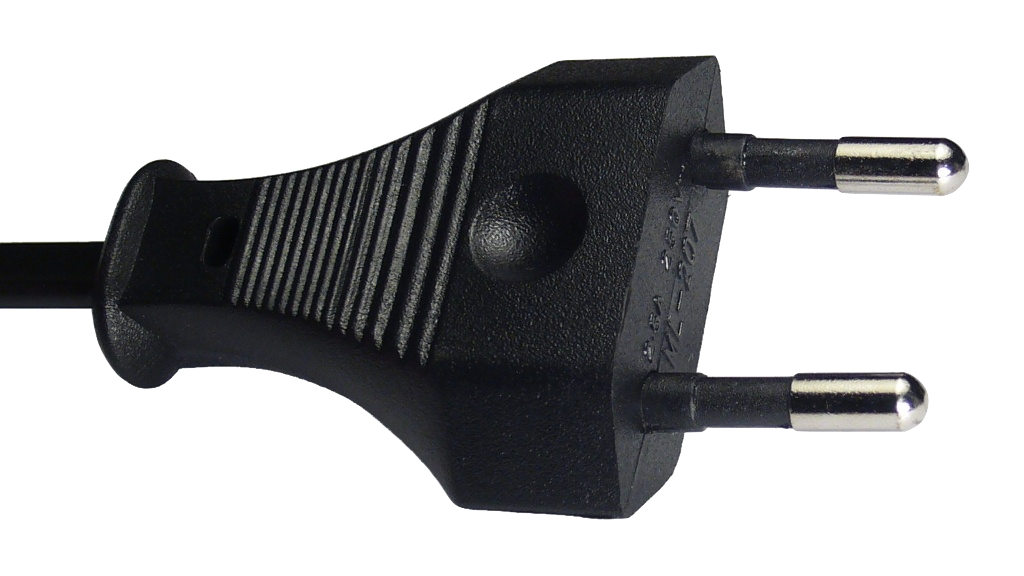
\includegraphics[width=2cm]{type_c.png}} \\
\addlinespace
\multicolumn{5}{l}{Classe I} \\
\middashrule
		& Matériel ayant une simple isolation mais présentant un dispositif de mise à la terre			& Ordinateur, lampadaire, fer à repasser, fer à souder\ldots		&  \multicolumn{1}{c}{\adjustbox{valign=t}{
\includegraphics[width=1cm]{classe_I.png}}} & \adjustbox{valign=t}{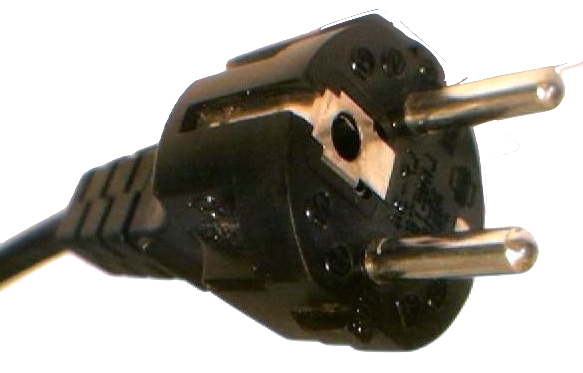
\includegraphics[width=2cm]{type_e.png}} \\
\noalign{\break} %impose le saut de page au tableau tout en répartissant verticalement le tableau
\addlinespace
\multicolumn{5}{l}{Classe II} \\
\middashrule		
		& Matériel présentant une double isolation de la partie active \Circled{1} (isolation fonctionnelle \Circled{2} et isolation supplémentaire \Circled{3}) ne nécessitant donc pas de mise à la terre			& Chaîne hi-fi, sèche-cheveux, rasoir électrique\ldots		& \multicolumn{1}{c}{\adjustbox{valign=t}{
\includegraphics[width=1cm]{classe_II.png}}}		& \adjustbox{valign=t}{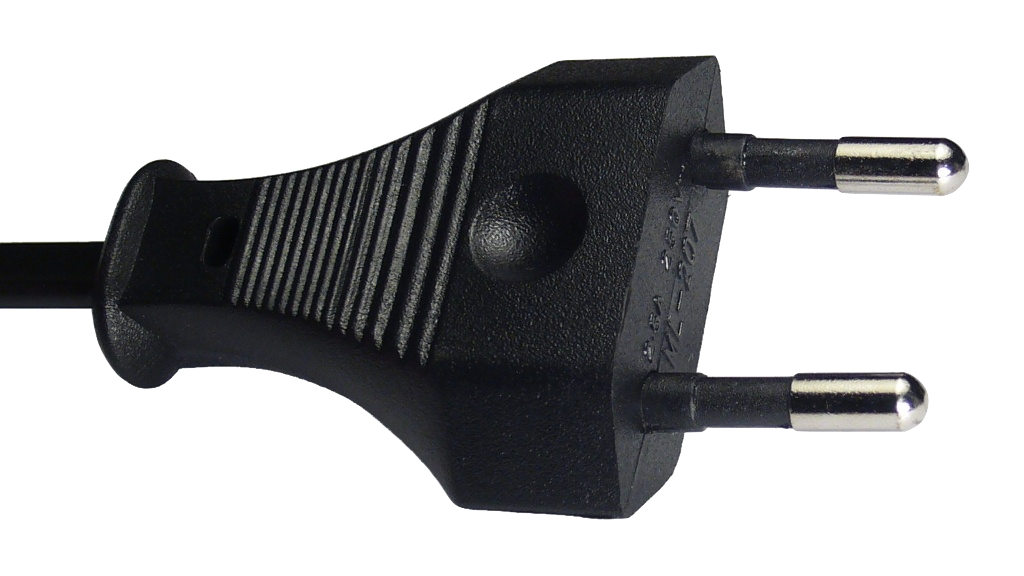
\includegraphics[width=2cm]{type_c.png}} \\
\addlinespace
\multicolumn{5}{l}{Classe III} \\
\middashrule		
		& Matériel ne fonctionnant qu'en très basse tension (\SI{12}{\volt}	ou \SI{24}{\volt}) et ne présentant pas de dangers pour les personnes (aucune précaution particulière à prendre)			& Circuits électriques, sonnette, smartphone\ldots		& \multicolumn{1}{c}{\adjustbox{valign=t}{
\includegraphics[width=1cm]{classe_III.png}}}		& \adjustbox{valign=t}{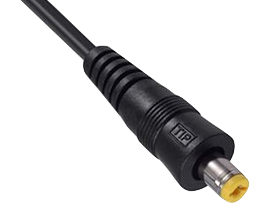
\includegraphics[width=2cm]{fiche_TBT.png}}
\end{xltabular}

\begin{figure}[h]
\caption{Matériel de classe d'isolation II} %lien éditeur Bruno Douchy : https://www.mathcha.io/editor/KxQmrUWBUm3TJwvgGohw0oEeWc2Mo9q7iLwLp4k
\tikzset{every picture/.style={line width=0.75pt}} %set default line width to 0.75pt        
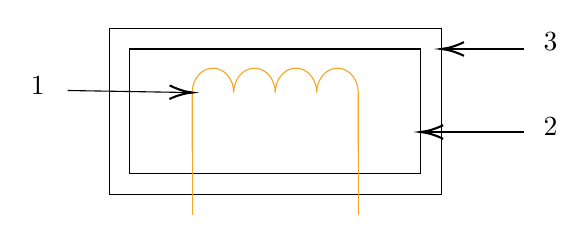
\begin{tikzpicture}[x=0.75pt,y=0.75pt,yscale=-1,xscale=1]
%uncomment if require: \path (0,300); %set diagram left start at 0, and has height of 300
%Shape: Rectangle [id:dp6431615116150586] 
\draw   (120,100) -- (260,100) -- (260,160) -- (120,160) -- cycle ;
%Shape: Rectangle [id:dp21722968746615745] 
\draw   (110,90) -- (270,90) -- (270,170) -- (110,170) -- cycle ;
%Shape: Inductor [id:dp2168804832907768] 
\draw  [color={rgb, 255:red, 245; green, 166; blue, 35 }  ,draw opacity=1 ] (150,149.24) -- (150,121) .. controls (150,114.51) and (154.48,109.24) .. (160,109.24) .. controls (165.52,109.24) and (170,114.51) .. (170,121) .. controls (170,114.51) and (174.48,109.24) .. (180,109.24) .. controls (185.52,109.24) and (190,114.51) .. (190,121) .. controls (190,114.51) and (194.48,109.24) .. (200,109.24) .. controls (205.52,109.24) and (210,114.51) .. (210,121) .. controls (210,114.51) and (214.48,109.24) .. (220,109.24) .. controls (225.52,109.24) and (230,114.51) .. (230,121) -- (230,149.24) ;
%Straight Lines [id:da9190346443391305] 
\draw [color={rgb, 255:red, 245; green, 166; blue, 35 }  ,draw opacity=1 ]   (150,149.24) -- (150,180) ;
%Straight Lines [id:da1556694134502471] 
\draw [color={rgb, 255:red, 245; green, 166; blue, 35 }  ,draw opacity=1 ]   (230,149.24) -- (230,180) ;
%Straight Lines [id:da6906822080495362] 
\draw    (90,120) -- (148,120.97) ;
\draw [shift={(150,121)}, rotate = 180.95] [color={rgb, 255:red, 0; green, 0; blue, 0 }  ][line width=0.75]    (10.93,-3.29) .. controls (6.95,-1.4) and (3.31,-0.3) .. (0,0) .. controls (3.31,0.3) and (6.95,1.4) .. (10.93,3.29)   ;
%Straight Lines [id:da8500651824334423] 
\draw    (310,100) -- (272,100) ;
\draw [shift={(270,100)}, rotate = 360] [color={rgb, 255:red, 0; green, 0; blue, 0 }  ][line width=0.75]    (10.93,-3.29) .. controls (6.95,-1.4) and (3.31,-0.3) .. (0,0) .. controls (3.31,0.3) and (6.95,1.4) .. (10.93,3.29)   ;
%Straight Lines [id:da6409885852889874] 
\draw    (310,140) -- (262,140) ;
\draw [shift={(260,140)}, rotate = 360] [color={rgb, 255:red, 0; green, 0; blue, 0 }  ][line width=0.75]    (10.93,-3.29) .. controls (6.95,-1.4) and (3.31,-0.3) .. (0,0) .. controls (3.31,0.3) and (6.95,1.4) .. (10.93,3.29)   ;

% Text Node
\draw (71,112) node [anchor=north west][inner sep=0.75pt]   [align=left] {\Circled{1}};
% Text Node
\draw (318,132) node [anchor=north west][inner sep=0.75pt]   [align=left] {\Circled{2}};
% Text Node
\draw (318,91) node [anchor=north west][inner sep=0.75pt]   [align=left] {\Circled{3}};
\end{tikzpicture}
\end{figure}


\subsection{Dispositif Différentiel Résiduel\label{subsec:DDR}}

\subsubsection{Caractéristiques générales}

\begin{definition}{Dispositif Différentiel Résiduel}{}
Un Dispositif Différentiel Résiduel (DDR) est un appareil de protection chargé d'assurer la protection des personnes contre les défauts d'isolement provoquant potentiellement des contacts indirects (\superref{def:contact_indirect}). Son rôle est de surveiller les fuites de courant d'une installation électrique vers la terre.
\end{definition}

Il convient de bien différencier deux type de DDR :
\begin{description}
\item[Interrupteur différentiel :] protection des personnes contre les contacts indirects dont le symbole est le suivant. \\
\begin{center}


\tikzset{every picture/.style={line width=0.75pt}} %set default line width to 0.75pt        

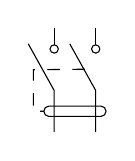
\begin{tikzpicture}[x=0.75pt,y=0.75pt,yscale=-1,xscale=1]
%uncomment if require: \path (0,300); %set diagram left start at 0, and has height of 300

%Straight Lines [id:da2903329919565012] 
\draw    (355,127.5) -- (367.5,150) -- (367.5,170) ;
%Shape: Circle [id:dp3187615529298826] 
\draw   (369.5,130) .. controls (369.5,128.9) and (368.6,128) .. (367.5,128) .. controls (366.4,128) and (365.5,128.9) .. (365.5,130) .. controls (365.5,131.1) and (366.4,132) .. (367.5,132) .. controls (368.6,132) and (369.5,131.1) .. (369.5,130) -- cycle ;
%Straight Lines [id:da6291068913098858] 
\draw    (367.5,128) -- (367.5,120) ;
%Rounded Rect [id:dp5228947876486602] 
\draw   (362.5,160) .. controls (362.5,158.62) and (363.62,157.5) .. (365,157.5) -- (390,157.5) .. controls (391.38,157.5) and (392.5,158.62) .. (392.5,160) -- (392.5,160) .. controls (392.5,161.38) and (391.38,162.5) .. (390,162.5) -- (365,162.5) .. controls (363.62,162.5) and (362.5,161.38) .. (362.5,160) -- cycle ;
%Straight Lines [id:da9535405775656056] 
\draw  [dash pattern={on 4.5pt off 4.5pt}]  (382.25,139.75) -- (357.5,140) -- (357.5,160) -- (362.5,160) ;
%Straight Lines [id:da293136389225495] 
\draw    (375,127.5) -- (387.5,150) -- (387.5,170) ;
%Shape: Circle [id:dp1387355280779735] 
\draw   (389.5,130) .. controls (389.5,128.9) and (388.6,128) .. (387.5,128) .. controls (386.4,128) and (385.5,128.9) .. (385.5,130) .. controls (385.5,131.1) and (386.4,132) .. (387.5,132) .. controls (388.6,132) and (389.5,131.1) .. (389.5,130) -- cycle ;
%Straight Lines [id:da810942314060853] 
\draw    (387.5,128) -- (387.5,120) ;

\end{tikzpicture}
\end{center}

\item[Disjoncteur différentiel :] protection des personnes contre les contacts indirects et protection des circuits contre les surintensités et les court-circuits dont le symbole est le suivant \\
\begin{center}


\tikzset{every picture/.style={line width=0.75pt}} %set default line width to 0.75pt        

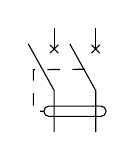
\begin{tikzpicture}[x=0.75pt,y=0.75pt,yscale=-1,xscale=1]
%uncomment if require: \path (0,300); %set diagram left start at 0, and has height of 300

%Straight Lines [id:da26208223112851936] 
\draw    (527.5,100) -- (540,122.5) -- (540,142.5) ;
%Straight Lines [id:da5822281275248988] 
\draw    (540,102.5) -- (540,92.5) ;
%Rounded Rect [id:dp41055324766610257] 
\draw   (535,132.5) .. controls (535,131.12) and (536.12,130) .. (537.5,130) -- (562.5,130) .. controls (563.88,130) and (565,131.12) .. (565,132.5) -- (565,132.5) .. controls (565,133.88) and (563.88,135) .. (562.5,135) -- (537.5,135) .. controls (536.12,135) and (535,133.88) .. (535,132.5) -- cycle ;
%Straight Lines [id:da30592283799275743] 
\draw  [dash pattern={on 4.5pt off 4.5pt}]  (554.75,112.25) -- (530,112.5) -- (530,132.5) -- (535,132.5) ;
%Straight Lines [id:da7841914077845515] 
\draw    (538,100.5) -- (542,104.5) ;
%Straight Lines [id:da01685582709758693] 
\draw    (542,100.5) -- (538,104.5) ;

%Straight Lines [id:da7197353055881572] 
\draw    (547.5,100) -- (560,122.5) -- (560,142.5) ;
%Straight Lines [id:da316262731013633] 
\draw    (560,102.5) -- (560,92.5) ;
%Straight Lines [id:da6806510311797901] 
\draw    (558,100.5) -- (562,104.5) ;
%Straight Lines [id:da5532087619463947] 
\draw    (562,100.5) -- (558,104.5) ;
\end{tikzpicture}

\end{center}
\end{description}

\begin{table}[h]
\caption{Valeur du seuil de $I_{\Delta n}$ fonction de $R_{A}$ et $U_{L}$}
\begin{tabularx}{\linewidth}{C i k S C i k S C i k S}
\toprule
\thead{$U_{L}$}	& \multicolumn{2}{c}{\thead{$R_{A}$ (\si{\ohm})}}	& 	{$I_{\Delta n}$ (\si{\ampere})}	& \thead{$U_{L}$}	& \multicolumn{2}{c}{\thead{$R_{A}$ (\si{\ohm})}}	& 	{$I_{\Delta n}$ (\si{\ampere})} & \thead{$U_{L}$}	& \multicolumn{2}{c}{\thead{$R_{A}$ (\si{\ohm})}}	& 	{$I_{\Delta n}$ (\si{\ampere})}	\\
\midrule
\SI{50}{\volt}	& \geq & 1660	&  0,030 		& \SI{25}{\volt}	& \geq & 500	& 	0,030	& \SI{12}{\volt}		& \geq & 400	&  0,030 \\
						& \geq & 166		&  0,300 		& 							& \geq & 83	&  0,300 	& 								& \geq & 40	&  0,300  \\
						& \geq & 100		&  0,500 		& 							& \geq & 50	&  0,500 	& 								& \geq & 24	&  0,500  \\
						& \geq & 16		&  3				& 							& \geq & 8		& 		 3 		& 								& \geq & 4		&  3  \\
\bottomrule
\end{tabularx}
\end{table}

\subsubsection{Marquage normalisé}

Comme tout appareil de protection, le DDR respecte des normes de qualité strictes (Conformité Européenne) et doivent présenter plusieurs marquages réglementaires, ainsi qu'un bouton \og TEST \fg{} pour informer l'installateur et l'utilisateur des caractéristiques du DDR. Cela informe de la conformité de l'appareil de protection.
\startcstep %remet les compteurs des légendes en pastille à zéro
\begin{center}
\begin{figure}[h]
\caption{Marquage d'un interrupteur différentiel}
\begin{subfigure}[t]{0.49\linewidth}
\subcaption{Vue de dessus}
\begin{annotate}
{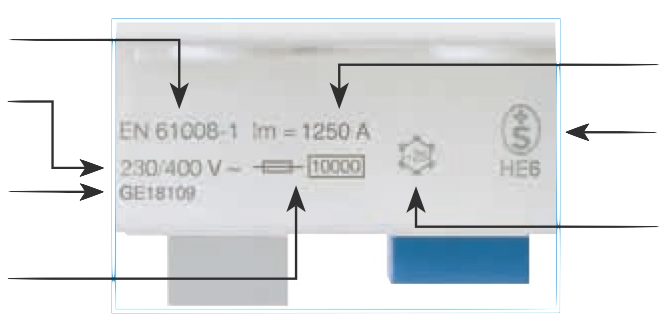
\includegraphics[scale=1]{DDR_dessus}}{0.25}
%\helpgrid[gray] 
\node at (-11.8,4.3) {\Circled{1}};
\node at (-11.8,2.2) {\Circled{2}};
\node at (-11.8,-0.85) {\Circled{3}};
\node at (-11.8,-3.85) {\Circled{4}};
\node at (11.7,3.4) {\Circled{5}};
\node at (11.7,1.1) {\Circled{6}};
\node at (11.7,-2.1) {\Circled{7}};
\end{annotate} 
\end{subfigure}
\begin{subfigure}[t]{0.49\linewidth}
\subcaption{Vue de dessus}
\begin{annotate}
{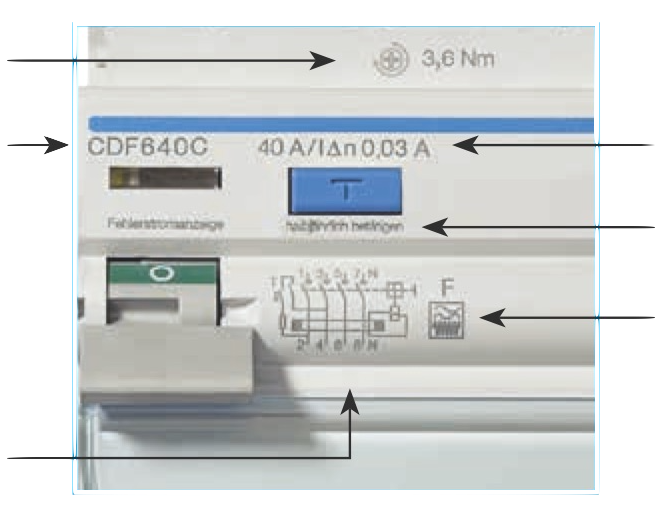
\includegraphics[scale=1]{DDR_avant}}{0.25}
%\helpgrid[gray] 
\node at (-11.8,6.7) {\Circled{8}};
\node at (-11.8,3.8) {\Circled{9}};
\node at (-11.9,-6.85) {\Circled{10}};
\node at (11.7,3.85) {\Circled{11}};
\node at (11.7,1) {\Circled{12}};
\node at (11.7,-2.05) {\Circled{13}};
\end{annotate} 
\end{subfigure}
\end{figure}
\end{center}
\begin{minipage}{\linewidth} %usage d'un environnement mini-page pour éviter les décalage au début de la première colonne quand l'élément n'est pas du texte simple
	\begin{multicols}{2} %répartition du texte dans l'environnement en deux colonnes
		\Circled{1} norme du produit\\ %légende automatique
		\Circled{2} tension assignée $230/400\si{\volt}\sim$\\
		\Circled{3} code de production\\
		\Circled{4} signe \og Courant assigné de court-circuit \SI{10000}{\ampere} \fg{} en combinaison avec un fusible en amont \\
		\Circled{5} pouvoir assigné de coupure \og \SI{1250}{\ampere} \fg{} \\
		\Circled{6} signe de sécurité ESTI (équivalent de la norme NF pour la Suisse) \\
		\Circled{7} signe \og Flocon de neige \fg{} (utilisation pour une température ambiante jusqu'à \SI{-25}{\degree}) \\
		\columnbreak\\ %passage à la deuxième colonne
		\Circled{8} couple de serrage \si{\newton\meter} \\
		\Circled{9} désignation du type\\
		\Circled{10} schéma des connexions\\
		\Circled{11} courant assigné $I_n$ de \SI{40}{\ampere} et calibre du DDR $I_{\Delta n}$\\
		\Circled{12} note concernant le test \og à effectuer tous les six mois \fg{}\\
		 \Circled{13} type de courant différentiel (type F)
	\end{multicols}
\end{minipage}


\subsubsection{Composante du courant de défaut}

Les DDR peuvent détecter plusieurs composantes du courant de défaut. C'est un paramètre qui peut varier selon le type d'appareil électrique protégé par le DDR.

%--------------------------------------
%ELECTROTECHNIQUE - SCHEMA DE LIAISON A LA TERRE
%--------------------------------------

%utiliser les environnement \begin{comment} \end{comment} pour mettre en commentaire le préambule une fois la programmation appelée dans le document maître (!ne pas oublier de mettre en commentaire \end{document}!)

\begin{comment}

\documentclass[a4paper, 11pt, twoside, fleqn]{memoir}

\usepackage{AOCDTF}

\marqueurchapitre

%lien d'édition des figures Tikz sur le site mathcha.io (rajouter le lien d'une modification effectuée sur la figure tikz avec le nom du modificateur car il n'y a qu'un lien par compte)

%lien éditeur Bruno Douchy : https://www.mathcha.io/editor/zjygnFElSdyhJ72e3zT5ZgqwBT4DKnovswpXn1q

%--------------------------------------
%corps du document
%--------------------------------------

\begin{document} %corps du document
	\openleft %début de chapitre à gauche

\end{comment}

\begin{xltabular}{\textwidth}{l c >{\compress}X c c }
\caption{Différents types de DDR selon les composantes du courant de défaut}\\
\toprule
\thead{Type}		& \thead{Symbole}		& \thead{Caractéristiques}	& \thead{Forme d'onde}		& \thead{Type de charge} \\
\midrule
\endfirsthead %en-tête de la première page du tableau  
\multicolumn{5}{l}{\small\textit{Page précédente}} \\
\midrule %filet de milieu de tableau
\thead{Type}		& \thead{Symbole}		& \thead{Caractéristiques}	& \thead{Forme d'onde}		& \thead{Type de charge} \\
\midrule
\endhead
\midrule %filet de milieu de tableau
\multicolumn{5}{r}{\small\textit{Page suivante}} \\
\endfoot %pied de page de toutes les pages du tableau
\bottomrule
\endlastfoot %pied de page de la dernièredu tableau
Type AC		& \adjustbox{valign=t}{
\includegraphics[height=0.4cm]{type_ac.png}}		& 
\begin{tabitemize}
\item détection des courants alternatifs différentiels\,;
\item utilisation courante en domestique couvrant la plupart des besoin.
\end{tabitemize}
&

\adjustbox{valign=t}{

\tikzset{every picture/.style={line width=0.75pt}} %set default line width to 0.75pt        

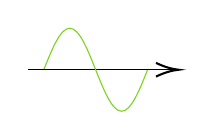
\begin{tikzpicture}[x=0.75pt,y=0.75pt,yscale=-1,xscale=1]
%uncomment if require: \path (0,57); %set diagram left start at 0, and has height of 57

%Straight Lines [id:da2943661507092279] 
\draw    (7.5,25) -- (78,25) ;
\draw [shift={(80,25)}, rotate = 180] [color={rgb, 255:red, 0; green, 0; blue, 0 }  ][line width=0.75]    (10.93,-3.29) .. controls (6.95,-1.4) and (3.31,-0.3) .. (0,0) .. controls (3.31,0.3) and (6.95,1.4) .. (10.93,3.29)   ;
%Shape: Wave [id:dp24323544196681968] 
\draw  [color={rgb, 255:red, 126; green, 211; blue, 33 }  ,draw opacity=1 ] (15,25) .. controls (19.08,14.75) and (22.98,5) .. (27.5,5) .. controls (32.02,5) and (35.92,14.75) .. (40,25) .. controls (44.08,35.25) and (47.98,45) .. (52.5,45) .. controls (57.02,45) and (60.92,35.25) .. (65,25) ;
%Straight Lines [id:da09599799976641754] 
\draw    (7.5,25) -- (30,25) ;
%Straight Lines [id:da7289357219255289] 
\draw    (43.75,25) -- (66.25,25) ;


\end{tikzpicture}}
 &
 
\adjustbox{valign=t}{


\tikzset{every picture/.style={line width=0.75pt}} %set default line width to 0.75pt        

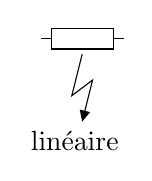
\begin{tikzpicture}[x=0.75pt,y=0.75pt,yscale=-1,xscale=1]
%uncomment if require: \path (0,98); %set diagram left start at 0, and has height of 98

%Straight Lines [id:da7324284340679806] 
\draw    (122.5,17.5) -- (127.5,17.5) ;
%Shape: Rectangle [id:dp18713096911447358] 
\draw   (92.5,12.5) -- (122.5,12.5) -- (122.5,22.5) -- (92.5,22.5) -- cycle ;
%Straight Lines [id:da2214074924221885] 
\draw    (87.5,17.5) -- (92.5,17.5) ;

%Straight Lines [id:da09102665939260723] 
\draw    (107.5,25) -- (102.5,45) -- (112.5,37.5) -- (108.23,54.59) ;
\draw [shift={(107.5,57.5)}, rotate = 284.04] [fill={rgb, 255:red, 0; green, 0; blue, 0 }  ][line width=0.08]  [draw opacity=0] (5.36,-2.57) -- (0,0) -- (5.36,2.57) -- cycle    ;

% Text Node
\draw (81.5,61) node [anchor=north west][inner sep=0.75pt]   [align=left] {linéaire};


\end{tikzpicture}}

  \\
    \addlinespace
  \addlinespace

  
  
  Type A		& \adjustbox{valign=t}{
\includegraphics[height=0.4cm]{type_a.png}}		& 
\begin{tabitemize}
\item détection des courants différentiels alternatifs et des courants différentiels continus pulsés\,;
\item utilisation spécifique pour les charges électriques monophasées de type 1.
\end{tabitemize}
&

\adjustbox{valign=t}{




\tikzset{every picture/.style={line width=0.75pt}} %set default line width to 0.75pt        

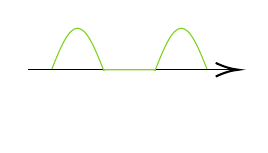
\begin{tikzpicture}[x=0.75pt,y=0.75pt,yscale=-1,xscale=1]
%uncomment if require: \path (0,108); %set diagram left start at 0, and has height of 108

%Shape: Wave [id:dp27700594343461393] 
\draw  [color={rgb, 255:red, 126; green, 211; blue, 33 }  ,draw opacity=1 ] (35,45) .. controls (39.08,34.75) and (42.98,25) .. (47.5,25) .. controls (52.02,25) and (55.92,34.75) .. (60,45) .. controls (64.08,55.25) and (67.98,65) .. (72.5,65) .. controls (77.02,65) and (80.92,55.25) .. (85,45) .. controls (89.08,34.75) and (92.98,25) .. (97.5,25) .. controls (102.02,25) and (105.92,34.75) .. (110,45) ;
%Straight Lines [id:da5910455205676639] 
\draw    (23.75,45) -- (123,45) ;
\draw [shift={(125,45)}, rotate = 180] [color={rgb, 255:red, 0; green, 0; blue, 0 }  ][line width=0.75]    (10.93,-3.29) .. controls (6.95,-1.4) and (3.31,-0.3) .. (0,0) .. controls (3.31,0.3) and (6.95,1.4) .. (10.93,3.29)   ;
%Straight Lines [id:da5095890041059973] 
\draw [color={rgb, 255:red, 126; green, 211; blue, 33 }  ,draw opacity=1 ]   (60,45) -- (85,45) ;
%Shape: Trapezoid [id:dp9576415302257589] 
\draw  [color={rgb, 255:red, 126; green, 211; blue, 33 }  ,draw opacity=1 ] (85,45) -- (84.7,46) -- (60.3,46) -- (60,45) -- cycle ;
%Shape: Rectangle [id:dp7690910497329457] 
\draw  [draw opacity=0][fill={rgb, 255:red, 255; green, 255; blue, 255 }  ,fill opacity=1 ][line width=5.25]  (35,45.5) -- (105,45.5) -- (105,68) -- (35,68) -- cycle ;




\end{tikzpicture}

}
 &
 
 
\adjustbox{valign=t}{



\tikzset{every picture/.style={line width=0.75pt}} %set default line width to 0.75pt        

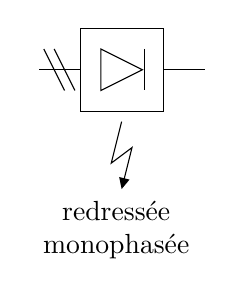
\begin{tikzpicture}[x=0.75pt,y=0.75pt,yscale=-1,xscale=1]
%uncomment if require: \path (0,152); %set diagram left start at 0, and has height of 152

%Straight Lines [id:da2993135281874989] 
\draw    (40,35) -- (30,15) ;
%Straight Lines [id:da1407255659834652] 
\draw    (35,35) -- (25,15) ;
%Straight Lines [id:da0646281171352201] 
\draw    (42.5,25) -- (22.5,25) ;
%Shape: Square [id:dp8095195384599084] 
\draw   (42.5,5) -- (82.5,5) -- (82.5,45) -- (42.5,45) -- cycle ;
%Shape: Boxed Line [id:dp9015036881777688] 
\draw    (73.5,15) -- (73.5,35) ;
%Shape: Triangle [id:dp25930553779074683] 
\draw   (72.5,25) -- (52.5,35) -- (52.5,15) -- cycle ;
%Straight Lines [id:da624315601423471] 
\draw    (62.5,50) -- (57.5,70) -- (67.5,62.5) -- (63.23,79.59) ;
\draw [shift={(62.5,82.5)}, rotate = 284.04] [fill={rgb, 255:red, 0; green, 0; blue, 0 }  ][line width=0.08]  [draw opacity=0] (5.36,-2.57) -- (0,0) -- (5.36,2.57) -- cycle    ;
%Straight Lines [id:da583175718122269] 
\draw    (102.5,25) -- (82.5,25) ;

% Text Node
\draw (17.5,87) node [anchor=north west][inner sep=0.75pt]   [align=left] {\begin{minipage}[lt]{61.699375pt}\setlength\topsep{0pt}
\begin{center}
redressée\\monophasée
\end{center}

\end{minipage}};


\end{tikzpicture}
}

  \\
    \addlinespace
  \addlinespace

  
    Type F		& \adjustbox{valign=t}{
\includegraphics[height=0.4cm]{type_f.png}}		& 
\begin{tabitemize}
\item détection des courants différentiels alternatifs, les courants différentiels continus pulsés et les courants différentiels de fréquences mixtes jusqu'à \SI{1}{\kilo\hertz}\,;
\item utilisation spécifique pour circuits comportant des variateurs de vitesse monophasés.
\end{tabitemize}
&

\adjustbox{valign=t}{
\tikzset{every picture/.style={line width=0.75pt}} %set default line width to 0.75pt        

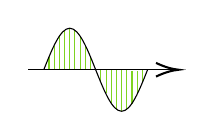
\begin{tikzpicture}[x=0.75pt,y=0.75pt,yscale=-1,xscale=1]
%uncomment if require: \path (0,108); %set diagram left start at 0, and has height of 108

%Straight Lines [id:da8344481258673822] 
\draw [color={rgb, 255:red, 126; green, 211; blue, 33 }  ,draw opacity=1 ]   (47.5,25) -- (47.5,45) ;
%Straight Lines [id:da45734535299498047] 
\draw [color={rgb, 255:red, 126; green, 211; blue, 33 }  ,draw opacity=1 ]   (45,26) -- (45,45) ;
%Straight Lines [id:da4148698837495829] 
\draw [color={rgb, 255:red, 126; green, 211; blue, 33 }  ,draw opacity=1 ]   (42.5,28.5) -- (42.5,44.5) ;
%Straight Lines [id:da9637733631041641] 
\draw [color={rgb, 255:red, 126; green, 211; blue, 33 }  ,draw opacity=1 ]   (37.5,39) -- (37.5,45) ;
%Straight Lines [id:da15505371109761856] 
\draw [color={rgb, 255:red, 126; green, 211; blue, 33 }  ,draw opacity=1 ]   (40,33.5) -- (40,44.5) ;
%Straight Lines [id:da8124028319543418] 
\draw [color={rgb, 255:red, 126; green, 211; blue, 33 }  ,draw opacity=1 ]   (52.5,29) -- (52.5,45) ;
%Straight Lines [id:da9805020896518191] 
\draw [color={rgb, 255:red, 126; green, 211; blue, 33 }  ,draw opacity=1 ]   (50,26) -- (50,45) ;
%Straight Lines [id:da4116431840997269] 
\draw [color={rgb, 255:red, 126; green, 211; blue, 33 }  ,draw opacity=1 ]   (55,34) -- (55,45) ;
%Straight Lines [id:da8823890585871352] 
\draw [color={rgb, 255:red, 126; green, 211; blue, 33 }  ,draw opacity=1 ]   (57.5,39) -- (57.5,45) ;
%Straight Lines [id:da9104778326348498] 
\draw [color={rgb, 255:red, 126; green, 211; blue, 33 }  ,draw opacity=1 ]   (72.5,65) -- (72.5,45) ;
%Straight Lines [id:da36879417192210706] 
\draw [color={rgb, 255:red, 126; green, 211; blue, 33 }  ,draw opacity=1 ]   (75,64) -- (75,45) ;
%Straight Lines [id:da056894793071553984] 
\draw [color={rgb, 255:red, 126; green, 211; blue, 33 }  ,draw opacity=1 ]   (77.5,61.5) -- (77.5,45.5) ;
%Straight Lines [id:da926320044180968] 
\draw [color={rgb, 255:red, 126; green, 211; blue, 33 }  ,draw opacity=1 ]   (82.5,51) -- (82.5,45) ;
%Straight Lines [id:da4802255081072313] 
\draw [color={rgb, 255:red, 126; green, 211; blue, 33 }  ,draw opacity=1 ]   (80,56.5) -- (80,45.5) ;
%Straight Lines [id:da8191961490083182] 
\draw [color={rgb, 255:red, 126; green, 211; blue, 33 }  ,draw opacity=1 ]   (67.5,61) -- (67.5,45) ;
%Straight Lines [id:da2923358818287347] 
\draw [color={rgb, 255:red, 126; green, 211; blue, 33 }  ,draw opacity=1 ]   (70,64) -- (70,45) ;
%Straight Lines [id:da3136693713803336] 
\draw [color={rgb, 255:red, 126; green, 211; blue, 33 }  ,draw opacity=1 ]   (65,56) -- (65,45) ;
%Straight Lines [id:da549046744886196] 
\draw [color={rgb, 255:red, 126; green, 211; blue, 33 }  ,draw opacity=1 ]   (62.5,51) -- (62.5,45) ;

%Shape: Wave [id:dp9341521104203707] 
\draw  [color={rgb, 255:red, 0; green, 0; blue, 0 }  ,draw opacity=1 ] (35,45) .. controls (39.08,34.75) and (42.98,25) .. (47.5,25) .. controls (52.02,25) and (55.92,34.75) .. (60,45) .. controls (64.08,55.25) and (67.98,65) .. (72.5,65) .. controls (77.02,65) and (80.92,55.25) .. (85,45) ;
%Straight Lines [id:da8093364598636541] 
\draw    (27.5,45) -- (98,45) ;
\draw [shift={(100,45)}, rotate = 180] [color={rgb, 255:red, 0; green, 0; blue, 0 }  ][line width=0.75]    (10.93,-3.29) .. controls (6.95,-1.4) and (3.31,-0.3) .. (0,0) .. controls (3.31,0.3) and (6.95,1.4) .. (10.93,3.29)   ;




\end{tikzpicture}

}
 &
 
 
\adjustbox{valign=t}{


\tikzset{every picture/.style={line width=0.75pt}} %set default line width to 0.75pt        

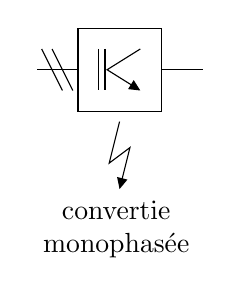
\begin{tikzpicture}[x=0.75pt,y=0.75pt,yscale=-1,xscale=1]
%uncomment if require: \path (0,152); %set diagram left start at 0, and has height of 152

%Straight Lines [id:da2004774518549749] 
\draw    (40,35) -- (30,15) ;
%Straight Lines [id:da28878490688185077] 
\draw    (35,35) -- (25,15) ;
%Straight Lines [id:da28622017833538005] 
\draw    (42.5,25) -- (22.5,25) ;
%Straight Lines [id:da27361779183994883] 
\draw    (62.5,50) -- (57.5,70) -- (67.5,62.5) -- (63.23,79.59) ;
\draw [shift={(62.5,82.5)}, rotate = 284.04] [fill={rgb, 255:red, 0; green, 0; blue, 0 }  ][line width=0.08]  [draw opacity=0] (5.36,-2.57) -- (0,0) -- (5.36,2.57) -- cycle    ;
%Straight Lines [id:da3667194527320474] 
\draw    (102.5,25) -- (82.5,25) ;
%Shape: Square [id:dp27983484657325586] 
\draw   (42.5,5) -- (82.5,5) -- (82.5,45) -- (42.5,45) -- cycle ;
%Shape: Boxed Line [id:dp856307990834614] 
\draw    (52.5,15) -- (52.5,35) ;
%Straight Lines [id:da34232786335443943] 
\draw    (72.5,15) -- (56.5,25) -- (69.96,33.41) ;
\draw [shift={(72.5,35)}, rotate = 212.01] [fill={rgb, 255:red, 0; green, 0; blue, 0 }  ][line width=0.08]  [draw opacity=0] (5.36,-2.57) -- (0,0) -- (5.36,2.57) -- cycle    ;
%Shape: Boxed Line [id:dp1790472061066909] 
\draw    (55.5,15) -- (55.5,35) ;


% Text Node
\draw (18.5,87) node [anchor=north west][inner sep=0.75pt]   [align=left] {\begin{minipage}[lt]{61.699375pt}\setlength\topsep{0pt}
\begin{center}
convertie\\monophasée
\end{center}

\end{minipage}};


\end{tikzpicture}

}

  \\
    \addlinespace
        \addlinespace


      Type B		& \adjustbox{valign=t}{
\includegraphics[height=0.4cm]{type_b.png}}		& 
\begin{tabitemize}
\item détection des courants différentiels alternatifs, les courants différentiels continus pulsés, des courants différentiels de fréquences mixtes jusqu'à \SI{1}{\kilo\hertz} et des courants différentiels continus lisses\,;
\item utilisation spécifique pour circuits comportant des variateurs de vitesse triphasés, un système photovoltaïque, une borne de recharge de véhicule électrique ou encore des équipements médicaux.
\end{tabitemize}
&

\adjustbox{valign=t}{


\tikzset{every picture/.style={line width=0.75pt}} %set default line width to 0.75pt        

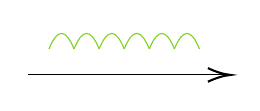
\begin{tikzpicture}[x=0.75pt,y=0.75pt,yscale=-1,xscale=1]
%uncomment if require: \path (0,108); %set diagram left start at 0, and has height of 108

%Straight Lines [id:da7026343722095999] 
\draw    (47.5,87.5) -- (143,87.5) ;
\draw [shift={(145,87.5)}, rotate = 180] [color={rgb, 255:red, 0; green, 0; blue, 0 }  ][line width=0.75]    (10.93,-3.29) .. controls (6.95,-1.4) and (3.31,-0.3) .. (0,0) .. controls (3.31,0.3) and (6.95,1.4) .. (10.93,3.29)   ;
%Shape: Parabola [id:dp4469234992699831] 
\draw  [color={rgb, 255:red, 126; green, 211; blue, 33 }  ,draw opacity=1 ] (69.58,75) .. controls (65.55,65) and (61.52,65) .. (57.5,75) ;
%Shape: Parabola [id:dp10691023078597706] 
\draw  [color={rgb, 255:red, 126; green, 211; blue, 33 }  ,draw opacity=1 ] (81.67,75) .. controls (77.64,65) and (73.61,65) .. (69.58,75) ;
%Shape: Parabola [id:dp9540942461898068] 
\draw  [color={rgb, 255:red, 126; green, 211; blue, 33 }  ,draw opacity=1 ] (93.75,75) .. controls (89.73,65) and (85.7,65) .. (81.67,75) ;
%Shape: Parabola [id:dp6220203064360257] 
\draw  [color={rgb, 255:red, 126; green, 211; blue, 33 }  ,draw opacity=1 ] (105.83,75) .. controls (101.8,65) and (97.77,65) .. (93.75,75) ;
%Shape: Parabola [id:dp4992966008122459] 
\draw  [color={rgb, 255:red, 126; green, 211; blue, 33 }  ,draw opacity=1 ] (117.92,75) .. controls (113.89,65) and (109.86,65) .. (105.83,75) ;
%Shape: Parabola [id:dp01154198803526707] 
\draw  [color={rgb, 255:red, 126; green, 211; blue, 33 }  ,draw opacity=1 ] (130,75) .. controls (125.98,65) and (121.95,65) .. (117.92,75) ;




\end{tikzpicture}

}
 &
 
 
\adjustbox{valign=t}{


\tikzset{every picture/.style={line width=0.75pt}} %set default line width to 0.75pt        

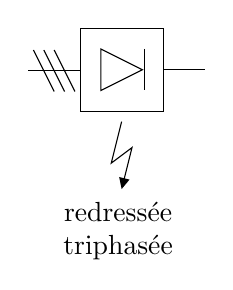
\begin{tikzpicture}[x=0.75pt,y=0.75pt,yscale=-1,xscale=1]
%uncomment if require: \path (0,141); %set diagram left start at 0, and has height of 141

%Straight Lines [id:da4147930693711671] 
\draw    (60,42.5) -- (50,22.5) ;
%Straight Lines [id:da7913487771488718] 
\draw    (55,42.5) -- (45,22.5) ;
%Straight Lines [id:da12782809797617567] 
\draw    (62.5,32.5) -- (37.5,32.5) ;
%Shape: Square [id:dp3051019253176962] 
\draw   (62.5,12) -- (102.5,12) -- (102.5,52) -- (62.5,52) -- cycle ;
%Shape: Boxed Line [id:dp3719227311734635] 
\draw    (93.5,22) -- (93.5,42) ;
%Shape: Triangle [id:dp5734231710257448] 
\draw   (92.5,32) -- (72.5,42) -- (72.5,22) -- cycle ;
%Straight Lines [id:da20189459286959577] 
\draw    (82.5,57) -- (77.5,77) -- (87.5,69.5) -- (83.23,86.59) ;
\draw [shift={(82.5,89.5)}, rotate = 284.04] [fill={rgb, 255:red, 0; green, 0; blue, 0 }  ][line width=0.08]  [draw opacity=0] (5.36,-2.57) -- (0,0) -- (5.36,2.57) -- cycle    ;
%Straight Lines [id:da8309944422064088] 
\draw    (122.5,32) -- (102.5,32) ;
%Straight Lines [id:da522665354082454] 
\draw    (50,42.5) -- (40,22.5) ;

% Text Node
\draw (47.5,94.5) node [anchor=north west][inner sep=0.75pt]   [align=left] {\begin{minipage}[lt]{48.078125pt}\setlength\topsep{0pt}
\begin{center}
redressée\\triphasée
\end{center}

\end{minipage}};


\end{tikzpicture}


}

  \\
  
\end{xltabular}


%\end{document}



\subsubsection{Principe de fonctionnement\label{subsubsec:principe_fonctionnement_ddr}}

Les éléments essentiels d'un DDR sont les suivants : \\
\begin{minipage}{\linewidth} %usage d'un environnement mini-page pour éviter les décalage au début de la première colonne quand l'élément n'est pas du texte simple
	\begin{multicols}{2} %répartition du texte dans l'environnement en deux colonnes
	\startcstep %remet les compteurs des légendes en pastille à zéro
		\Circled{1} bouton test d'essai du DDR\\ %légende automatique
		\Circled{2} transformateur d'intensité (tore de détection)\\
		\Circled{3} relais de déclenchement  \\
		\Circled{4} mécanisme à déclenchement libre sans retour automatique \\
		\columnbreak\\ %passage à la deuxième colonne
		$I_1$ : courant \og d'arrivée \fg{} du récepteur \\
		$I_2$ : courant \og de sortie \fg{} du récepteur \\
		$I_d$ : courant de défaut\\
		$I_c$ : courant de contact\\
		$R_B$ : résistance de terre du neutre\\
		$R_A$ : résistance de la prise de terre de l'installation électrique 
	\end{multicols}
\end{minipage}
~\\
Pour le fonctionnement d'un DDR, les conditions suivantes doivent être remplie :
\begin{itemize}
\item le point neutre du transformateur HT/BT doit être mis à la terre\,;
\item aucune liaison entre le conducteur de neutre et le conducteur de protection ne doit être réalisée en aval du DDR\,;
\item le conducteur de protection ne doit pas transiter dans le transformateur d'intensité\,;
\item le réseau doit être alternatif.
\end{itemize}

%--------------------------------------
%ELECTROTECHNIQUE - SCHEMA DE LIAISON A LA TERRE
%--------------------------------------

%utiliser les environnement \begin{comment} \end{comment} pour mettre en commentaire le préambule une fois la programmation appelée dans le document maître (!ne pas oublier de mettre en commentaire \end{document}!)

\begin{comment}

\documentclass[a4paper, 11pt, twoside, fleqn]{memoir}

\usepackage{AOCDTF}

%--------------------------------------
%CANEVAS
%--------------------------------------

\newcommand\BoxColor{\ifcase\thechapshift blue!30\or brown!30\or pink!30\or cyan!30\or green!30\or teal!30\or purple!30\or red!30\or olive!30\or orange!30\or lime!30\or gray!\or magenta!30\else yellow!30\fi} %définition de la couleur des marqueurs de chapitre

\newcounter{chapshift} %compteur de chapitre du marqueur de chapitre
\addtocounter{chapshift}{-1}
	
\newif\ifFrame %instruction conditionnelle pour les couleurs des pages
\Frametrue

\pagestyle{plain}

% the main command; the mandatory argument sets the color of the vertical box
\newcommand\ChapFrame{%
\AddEverypageHook{%
\ifFrame
\ifthenelse{\isodd{\value{page}}}
  {\backgroundsetup{contents={%
  \begin{tikzpicture}[overlay,remember picture]
  \node[
  	rounded corners=3pt,
    fill=\BoxColor,
    inner sep=0pt,
    rectangle,
    text width=1.5cm,
    text height=5.5cm,
    align=center,
    anchor=north west
  ] 
  at ($ (current page.north west) + (-0cm,-2*\thechapshift cm) $) %nombre négatif = espacement des marqueurs entre les différents chapitres (à régler en fin de rédaction) (4.5cm vaut un espacement équivalement à la hauteur du marqueur, une page peut en contenir 6 avec cet espacement-la mais il est le plus équilibré)
    {\rotatebox{90}{\hspace*{.5cm}%
      \parbox[c][1.2cm][t]{5cm}{%
        \raggedright\textcolor{black}{\sffamily\textbf{\leftmark}}}}};
  \end{tikzpicture}}}
  }
  {\backgroundsetup{contents={%
  \begin{tikzpicture}[overlay,remember picture]
  \node[
  	rounded corners=3pt,
    fill=\BoxColor,
    inner sep=0pt,
    rectangle,
    text width=1.5cm,
    text height=5.5cm,
    align=center,
    anchor=north east
  ] 
  at ($ (current page.north east) + (-0cm,-2*\thechapshift cm) $) %nombre négatif = espacement des marqueurs entre les différents chapitres (à régler en fin de rédaction) (4.5cm vaut un espacement équivalement à la hauteur du marqueur, une page peut en contenir 6 avec cet espacement-la mais il est le plus équilibré)
    {\rotatebox{90}{\hspace*{.5cm}%
      \parbox[c][1.2cm][t]{5cm}{%
        \raggedright\textcolor{black}{\sffamily\textbf{\leftmark}}}}};
  \end{tikzpicture}}}%
  }
  \BgMaterial%
  \fi%
}%
  \stepcounter{chapshift}
}

\renewcommand\chaptermark[1]{\markboth{\thechapter.~#1}{}} %redéfinition du marqueur de chapitre pour ne contenir que le titre du chapitre %à personnaliser selon le nombre de chapitre dans le cours

%--------------------------------------
%corps du document
%--------------------------------------

\begin{document} %corps du document
	\openleft %début de chapitre à gauche

\end{comment}

\begin{figure}[h]
\caption{Principe de fonctionnement d'un DDR}



% Pattern Info
 
\tikzset{
pattern size/.store in=\mcSize, 
pattern size = 5pt,
pattern thickness/.store in=\mcThickness, 
pattern thickness = 0.3pt,
pattern radius/.store in=\mcRadius, 
pattern radius = 1pt}
\makeatletter
\pgfutil@ifundefined{pgf@pattern@name@_uf0m8v139}{
\pgfdeclarepatternformonly[\mcThickness,\mcSize]{_uf0m8v139}
{\pgfqpoint{0pt}{0pt}}
{\pgfpoint{\mcSize+\mcThickness}{\mcSize+\mcThickness}}
{\pgfpoint{\mcSize}{\mcSize}}
{
\pgfsetcolor{\tikz@pattern@color}
\pgfsetlinewidth{\mcThickness}
\pgfpathmoveto{\pgfqpoint{0pt}{0pt}}
\pgfpathlineto{\pgfpoint{\mcSize+\mcThickness}{\mcSize+\mcThickness}}
\pgfusepath{stroke}
}}
\makeatother
\tikzset{every picture/.style={line width=0.75pt}} %set default line width to 0.75pt        

\begin{tikzpicture}[x=0.75pt,y=0.75pt,yscale=-1,xscale=1]
%uncomment if require: \path (0,424); %set diagram left start at 0, and has height of 424

%Straight Lines [id:da5569675718372048] 
\draw [color={rgb, 255:red, 248; green, 231; blue, 28 }  ,draw opacity=1 ]   (87.5,347.5) -- (87.5,372.5) ;
%Straight Lines [id:da8030717374799764] 
\draw [color={rgb, 255:red, 248; green, 231; blue, 28 }  ,draw opacity=1 ]   (222.5,260) -- (207.5,260) -- (207.5,307.5) ;
%Straight Lines [id:da7987961384438291] 
\draw    (170.5,77) -- (192.5,75) -- (202.5,75) ;
%Straight Lines [id:da08643413697598168] 
\draw    (172.5,75) -- (162.5,75) ;
%Straight Lines [id:da803548488580716] 
\draw    (170.5,77) -- (174.5,73) ;
%Straight Lines [id:da5481908490512861] 
\draw    (170.5,73) -- (174.5,77) ;

%Straight Lines [id:da26895957675314053] 
\draw    (170.5,57) -- (192.5,55) -- (202.5,55) ;
%Straight Lines [id:da6898264055807402] 
\draw    (172.5,55) -- (162.5,55) ;
%Straight Lines [id:da33859677367548024] 
\draw    (170.5,57) -- (174.5,53) ;
%Straight Lines [id:da5071692293587962] 
\draw    (170.5,53) -- (174.5,57) ;

%Straight Lines [id:da25810887146839223] 
\draw  [dash pattern={on 4.5pt off 4.5pt}]  (181.5,76) -- (181.5,16) ;
%Straight Lines [id:da3623003405229671] 
\draw    (170.5,37) -- (192.5,35) -- (202.5,35) ;
%Straight Lines [id:da4691855208617536] 
\draw    (172.5,35) -- (162.5,35) ;
%Straight Lines [id:da2705192532340027] 
\draw    (170.5,37) -- (174.5,33) ;
%Straight Lines [id:da5270698146878778] 
\draw    (170.5,33) -- (174.5,37) ;

%Straight Lines [id:da5208295098976554] 
\draw    (170.5,17) -- (192.5,15) -- (202.5,15) ;
%Straight Lines [id:da9100116120443311] 
\draw    (172.5,15) -- (162.5,15) ;
%Straight Lines [id:da07340037609998551] 
\draw    (170.5,17) -- (174.5,13) ;
%Straight Lines [id:da727439087554878] 
\draw    (170.5,13) -- (174.5,17) ;


%Straight Lines [id:da7894327394796508] 
\draw    (120,35) -- (162.5,35) ;
%Straight Lines [id:da6671442734999171] 
\draw [color={rgb, 255:red, 139; green, 87; blue, 42 }  ,draw opacity=1 ]   (112.5,15) -- (162.5,15) ;
%Straight Lines [id:da16231501811449245] 
\draw [color={rgb, 255:red, 155; green, 155; blue, 155 }  ,draw opacity=1 ]   (112.5,55) -- (162.5,55) ;
%Straight Lines [id:da04476213273823848] 
\draw [color={rgb, 255:red, 74; green, 144; blue, 226 }  ,draw opacity=1 ]   (87.5,75) -- (162.5,75) ;
%Straight Lines [id:da2559241348150122] 
\draw [color={rgb, 255:red, 248; green, 231; blue, 28 }  ,draw opacity=1 ]   (95.5,35) -- (87.5,65) -- (87.5,307.5) ;
%Straight Lines [id:da8531850209376354] 
\draw [color={rgb, 255:red, 126; green, 211; blue, 33 }  ,draw opacity=1 ] [dash pattern={on 4.5pt off 4.5pt}]  (95.5,35) -- (87.5,65) -- (87.5,161.33) -- (87.5,307.5) ;
%Shape: Circle [id:dp47194931654687355] 
\draw  [fill={rgb, 255:red, 0; green, 0; blue, 0 }  ,fill opacity=1 ] (85,75) .. controls (85,73.62) and (86.12,72.5) .. (87.5,72.5) .. controls (88.88,72.5) and (90,73.62) .. (90,75) .. controls (90,76.38) and (88.88,77.5) .. (87.5,77.5) .. controls (86.12,77.5) and (85,76.38) .. (85,75) -- cycle ;
%Straight Lines [id:da12418542898468488] 
\draw    (202.5,35) -- (460,35) ;
%Straight Lines [id:da892541875072728] 
\draw [color={rgb, 255:red, 139; green, 87; blue, 42 }  ,draw opacity=1 ]   (202.5,15) -- (460,15) ;
%Straight Lines [id:da742409178470536] 
\draw [color={rgb, 255:red, 155; green, 155; blue, 155 }  ,draw opacity=1 ]   (202.5,55) -- (460,55) ;
%Straight Lines [id:da856527021466942] 
\draw [color={rgb, 255:red, 74; green, 144; blue, 226 }  ,draw opacity=1 ]   (202.5,75) -- (460,75) ;
%Shape: Path Data [id:dp19593575615064884] 
\draw   (112.5,55) .. controls (112.5,56.38) and (111.38,57.5) .. (110,57.5) .. controls (109.29,57.5) and (108.65,57.2) .. (108.19,56.72) .. controls (102.81,61.85) and (95.52,65) .. (87.5,65) .. controls (70.93,65) and (57.5,51.57) .. (57.5,35) .. controls (57.5,18.43) and (70.93,5) .. (87.5,5) .. controls (95.52,5) and (102.81,8.15) .. (108.19,13.28) .. controls (108.65,12.8) and (109.29,12.5) .. (110,12.5) .. controls (111.38,12.5) and (112.5,13.62) .. (112.5,15) .. controls (112.5,15.82) and (112.11,16.54) .. (111.5,17) .. controls (114.8,21.39) and (116.92,26.71) .. (117.4,32.5) .. controls (117.43,32.5) and (117.47,32.5) .. (117.5,32.5) .. controls (118.88,32.5) and (120,33.62) .. (120,35) .. controls (120,36.38) and (118.88,37.5) .. (117.5,37.5) .. controls (117.47,37.5) and (117.43,37.5) .. (117.4,37.5) .. controls (116.92,43.29) and (114.8,48.61) .. (111.5,53) .. controls (112.11,53.46) and (112.5,54.18) .. (112.5,55) -- cycle ;
%Shape: Circle [id:dp7917428977896803] 
\draw   (17.5,35) .. controls (17.5,18.43) and (30.93,5) .. (47.5,5) .. controls (64.07,5) and (77.5,18.43) .. (77.5,35) .. controls (77.5,51.57) and (64.07,65) .. (47.5,65) .. controls (30.93,65) and (17.5,51.57) .. (17.5,35) -- cycle ;
%Shape: Triangle [id:dp8517252312032021] 
\draw   (40,25) -- (30,42.5) -- (50,42.5) -- cycle ;
%Shape: Star [id:dp07223973274580164] 
\draw   (106.75,35) -- (95.5,35) -- (89.88,44.81) -- (95.5,35) -- (89.88,25.19) -- (95.5,35) -- cycle ;
%Shape: Circle [id:dp389562574882782] 
\draw   (107.5,15) .. controls (107.5,13.62) and (108.62,12.5) .. (110,12.5) .. controls (111.38,12.5) and (112.5,13.62) .. (112.5,15) .. controls (112.5,16.38) and (111.38,17.5) .. (110,17.5) .. controls (108.62,17.5) and (107.5,16.38) .. (107.5,15) -- cycle ;
%Shape: Circle [id:dp684435310402229] 
\draw   (114.9,35) .. controls (114.9,33.62) and (116.02,32.5) .. (117.4,32.5) .. controls (118.78,32.5) and (119.9,33.62) .. (119.9,35) .. controls (119.9,36.38) and (118.78,37.5) .. (117.4,37.5) .. controls (116.02,37.5) and (114.9,36.38) .. (114.9,35) -- cycle ;
%Shape: Circle [id:dp060632852060490405] 
\draw   (107.5,55) .. controls (107.5,53.62) and (108.62,52.5) .. (110,52.5) .. controls (111.38,52.5) and (112.5,53.62) .. (112.5,55) .. controls (112.5,56.38) and (111.38,57.5) .. (110,57.5) .. controls (108.62,57.5) and (107.5,56.38) .. (107.5,55) -- cycle ;

%Shape: Circle [id:dp7102546693671166] 
\draw  [fill={rgb, 255:red, 0; green, 0; blue, 0 }  ,fill opacity=1 ] (250,15) .. controls (250,13.62) and (251.12,12.5) .. (252.5,12.5) .. controls (253.88,12.5) and (255,13.62) .. (255,15) .. controls (255,16.38) and (253.88,17.5) .. (252.5,17.5) .. controls (251.12,17.5) and (250,16.38) .. (250,15) -- cycle ;
%Shape: Circle [id:dp19881952558692362] 
\draw  [fill={rgb, 255:red, 0; green, 0; blue, 0 }  ,fill opacity=1 ] (290,75) .. controls (290,73.62) and (291.12,72.5) .. (292.5,72.5) .. controls (293.88,72.5) and (295,73.62) .. (295,75) .. controls (295,76.38) and (293.88,77.5) .. (292.5,77.5) .. controls (291.12,77.5) and (290,76.38) .. (290,75) -- cycle ;
%Straight Lines [id:da9609078171715071] 
\draw [color={rgb, 255:red, 74; green, 144; blue, 226 }  ,draw opacity=1 ]   (292.5,87.5) -- (292.5,77.5) ;
%Shape: Circle [id:dp9105511499855616] 
\draw   (290,90) .. controls (290,88.62) and (291.12,87.5) .. (292.5,87.5) .. controls (293.88,87.5) and (295,88.62) .. (295,90) .. controls (295,91.38) and (293.88,92.5) .. (292.5,92.5) .. controls (291.12,92.5) and (290,91.38) .. (290,90) -- cycle ;
%Straight Lines [id:da90253425713718] 
\draw [color={rgb, 255:red, 139; green, 87; blue, 42 }  ,draw opacity=1 ]   (252.5,87.5) -- (252.5,17.5) ;
%Shape: Circle [id:dp04612564222174287] 
\draw   (250,90) .. controls (250,88.62) and (251.12,87.5) .. (252.5,87.5) .. controls (253.88,87.5) and (255,88.62) .. (255,90) .. controls (255,91.38) and (253.88,92.5) .. (252.5,92.5) .. controls (251.12,92.5) and (250,91.38) .. (250,90) -- cycle ;
%Straight Lines [id:da41167791429417944] 
\draw    (249.5,110) -- (252.5,132.5) -- (252.5,142.5) ;
%Shape: Circle [id:dp9887333606589835] 
\draw   (254.5,112.5) .. controls (254.5,111.4) and (253.6,110.5) .. (252.5,110.5) .. controls (251.4,110.5) and (250.5,111.4) .. (250.5,112.5) .. controls (250.5,113.6) and (251.4,114.5) .. (252.5,114.5) .. controls (253.6,114.5) and (254.5,113.6) .. (254.5,112.5) -- cycle ;
%Straight Lines [id:da017525658811769262] 
\draw    (252.5,110.5) -- (252.5,102.5) ;
%Straight Lines [id:da9547976914347267] 
\draw [color={rgb, 255:red, 139; green, 87; blue, 42 }  ,draw opacity=1 ]   (252.5,102.5) -- (252.5,92.5) ;
%Straight Lines [id:da6837922838053284] 
\draw [color={rgb, 255:red, 74; green, 144; blue, 226 }  ,draw opacity=1 ]   (292.5,102.5) -- (292.5,92.5) ;
%Shape: Circle [id:dp01870989194207895] 
\draw   (294.5,112.5) .. controls (294.5,111.4) and (293.6,110.5) .. (292.5,110.5) .. controls (291.4,110.5) and (290.5,111.4) .. (290.5,112.5) .. controls (290.5,113.6) and (291.4,114.5) .. (292.5,114.5) .. controls (293.6,114.5) and (294.5,113.6) .. (294.5,112.5) -- cycle ;
%Straight Lines [id:da8844727625408757] 
\draw    (292.5,110.5) -- (292.5,102.5) ;
%Shape: Can [id:dp6490213632428469] 
\draw   (313,173.75) -- (313,186.25) .. controls (313,189.7) and (296.21,192.5) .. (275.5,192.5) .. controls (254.79,192.5) and (238,189.7) .. (238,186.25) -- (238,173.75) .. controls (238,170.3) and (254.79,167.5) .. (275.5,167.5) .. controls (296.21,167.5) and (313,170.3) .. (313,173.75) .. controls (313,177.2) and (296.21,180) .. (275.5,180) .. controls (254.79,180) and (238,177.2) .. (238,173.75) ;
%Shape: Ellipse [id:dp08313926467548194] 
\draw   (247.5,173) .. controls (247.5,170.79) and (259.81,169) .. (275,169) .. controls (290.19,169) and (302.5,170.79) .. (302.5,173) .. controls (302.5,175.21) and (290.19,177) .. (275,177) .. controls (259.81,177) and (247.5,175.21) .. (247.5,173) -- cycle ;
%Straight Lines [id:da06299666022161243] 
\draw    (289.5,110) -- (292.5,132.5) -- (292.5,142.5) ;
%Straight Lines [id:da8960645371105965] 
\draw [color={rgb, 255:red, 74; green, 144; blue, 226 }  ,draw opacity=1 ]   (292.5,175) -- (292.5,142.5) ;
%Straight Lines [id:da33101665629205235] 
\draw [color={rgb, 255:red, 139; green, 87; blue, 42 }  ,draw opacity=1 ]   (252.5,175) -- (252.5,142.5) ;
%Curve Lines [id:da3927543802796932] 
\draw [color={rgb, 255:red, 139; green, 87; blue, 42 }  ,draw opacity=1 ]   (249.5,175) .. controls (235.5,163) and (231.5,201) .. (242.5,190) ;
%Curve Lines [id:da10409159561355674] 
\draw [color={rgb, 255:red, 139; green, 87; blue, 42 }  ,draw opacity=1 ]   (252.5,176) .. controls (239.5,163) and (232.5,203) .. (245.5,190) ;
%Curve Lines [id:da6914928143797353] 
\draw [color={rgb, 255:red, 139; green, 87; blue, 42 }  ,draw opacity=1 ]   (255.5,176.5) .. controls (248.83,169.83) and (244.01,176.71) .. (242.51,183.45) .. controls (241.08,189.84) and (242.66,196.1) .. (248.5,190.5) ;
%Curve Lines [id:da7079333037592989] 
\draw [color={rgb, 255:red, 139; green, 87; blue, 42 }  ,draw opacity=1 ]   (248,172.5) .. controls (235,161.5) and (229,199.5) .. (240,188.5) ;
%Curve Lines [id:da057383623538654116] 
\draw [color={rgb, 255:red, 139; green, 87; blue, 42 }  ,draw opacity=1 ]   (247.5,173) .. controls (236.5,159.67) and (227.5,194.67) .. (236,188.25) ;
%Curve Lines [id:da22578986553009184] 
\draw [color={rgb, 255:red, 74; green, 144; blue, 226 }  ,draw opacity=1 ]   (294.11,174.52) .. controls (309.55,161.29) and (313.96,203.18) .. (301.83,191.05) ;
%Curve Lines [id:da6186372251586958] 
\draw [color={rgb, 255:red, 74; green, 144; blue, 226 }  ,draw opacity=1 ]   (290.81,175.62) .. controls (305.14,161.29) and (312.85,205.38) .. (298.52,191.05) ;
%Curve Lines [id:da40281426858450187] 
\draw [color={rgb, 255:red, 74; green, 144; blue, 226 }  ,draw opacity=1 ]   (287.5,176.17) .. controls (294.85,168.82) and (300.17,176.41) .. (301.82,183.83) .. controls (303.39,190.88) and (301.66,197.78) .. (295.22,191.6) ;
%Curve Lines [id:da2860637717642769] 
\draw [color={rgb, 255:red, 74; green, 144; blue, 226 }  ,draw opacity=1 ]   (295.77,171.76) .. controls (310.1,159.64) and (316.71,201.52) .. (304.59,189.4) ;
%Curve Lines [id:da004580586199153358] 
\draw [color={rgb, 255:red, 74; green, 144; blue, 226 }  ,draw opacity=1 ]   (296.77,172.76) .. controls (308.89,158.06) and (317.81,195.65) .. (308.44,188.57) ;
%Straight Lines [id:da18006882444959194] 
\draw [color={rgb, 255:red, 139; green, 87; blue, 42 }  ,draw opacity=1 ]   (252.5,210) -- (252.5,192) ;
%Straight Lines [id:da6899639114106388] 
\draw [color={rgb, 255:red, 74; green, 144; blue, 226 }  ,draw opacity=1 ]   (292.5,210) -- (292.5,192) ;
%Shape: Circle [id:dp023617772776452384] 
\draw   (290,240) .. controls (290,238.62) and (291.12,237.5) .. (292.5,237.5) .. controls (293.88,237.5) and (295,238.62) .. (295,240) .. controls (295,241.38) and (293.88,242.5) .. (292.5,242.5) .. controls (291.12,242.5) and (290,241.38) .. (290,240) -- cycle ;
%Shape: Circle [id:dp4247495564213074] 
\draw   (250,240) .. controls (250,238.62) and (251.12,237.5) .. (252.5,237.5) .. controls (253.88,237.5) and (255,238.62) .. (255,240) .. controls (255,241.38) and (253.88,242.5) .. (252.5,242.5) .. controls (251.12,242.5) and (250,241.38) .. (250,240) -- cycle ;
%Straight Lines [id:da41836049222392757] 
\draw [color={rgb, 255:red, 139; green, 87; blue, 42 }  ,draw opacity=1 ]   (252.5,255) -- (252.5,242.5) ;
%Straight Lines [id:da8111963186758367] 
\draw [color={rgb, 255:red, 74; green, 144; blue, 226 }  ,draw opacity=1 ]   (292.5,255.5) -- (292.5,242.5) ;
%Straight Lines [id:da7572420158424509] 
\draw    (45,285) -- (460,285) ;
%Shape: Rectangle [id:dp18411529638071378] 
\draw  [draw opacity=0][pattern=_uf0m8v139,pattern size=6pt,pattern thickness=0.75pt,pattern radius=0pt, pattern color={rgb, 255:red, 0; green, 0; blue, 0}][line width=0.75]  (45,285) -- (460,285) -- (460,300) -- (45,300) -- cycle ;
%Straight Lines [id:da03392621889598857] 
\draw [color={rgb, 255:red, 126; green, 211; blue, 33 }  ,draw opacity=1 ] [dash pattern={on 4.5pt off 4.5pt}]  (222.5,260) -- (207.5,260) -- (207.5,307.5) ;
%Shape: Circle [id:dp7571916793300425] 
\draw   (222.5,260) .. controls (222.5,258.62) and (223.62,257.5) .. (225,257.5) .. controls (226.38,257.5) and (227.5,258.62) .. (227.5,260) .. controls (227.5,261.38) and (226.38,262.5) .. (225,262.5) .. controls (223.62,262.5) and (222.5,261.38) .. (222.5,260) -- cycle ;
%Straight Lines [id:da20553450120643402] 
\draw    (87.5,372.5) -- (87.5,387.5) ;
%Straight Lines [id:da9544857402361856] 
\draw    (77.5,387.5) -- (97.5,387.5) ;
%Straight Lines [id:da6836120465702779] 
\draw    (80,392.5) -- (95,392.5) ;
%Straight Lines [id:da5098314930953095] 
\draw    (82.5,397.5) -- (92.5,397.5) ;

%Straight Lines [id:da14748133582745382] 
\draw [color={rgb, 255:red, 126; green, 211; blue, 33 }  ,draw opacity=1 ] [dash pattern={on 4.5pt off 4.5pt}]  (87.5,347.5) -- (87.5,372.5) ;
%Straight Lines [id:da07788601461052536] 
\draw [color={rgb, 255:red, 248; green, 231; blue, 28 }  ,draw opacity=1 ]   (207.5,347.5) -- (207.5,372.5) ;
%Straight Lines [id:da077984621762062] 
\draw    (207.5,372.5) -- (207.5,387.5) ;
%Straight Lines [id:da01964510614427828] 
\draw    (197.5,387.5) -- (217.5,387.5) ;
%Straight Lines [id:da29977229045078546] 
\draw    (200,392.5) -- (215,392.5) ;
%Straight Lines [id:da6901624132325382] 
\draw    (202.5,397.5) -- (212.5,397.5) ;

%Straight Lines [id:da32226465457516273] 
\draw [color={rgb, 255:red, 126; green, 211; blue, 33 }  ,draw opacity=1 ] [dash pattern={on 4.5pt off 4.5pt}]  (207.5,347.5) -- (207.5,372.5) ;
%Straight Lines [id:da2085284947671493] 
\draw    (287.5,255) -- (292.5,255) ;
%Shape: Rectangle [id:dp3078829888067669] 
\draw   (257.5,250) -- (287.5,250) -- (287.5,260) -- (257.5,260) -- cycle ;
%Straight Lines [id:da04494606262403944] 
\draw    (252.5,255) -- (257.5,255) ;

%Straight Lines [id:da42571296006378045] 
\draw  [thin, dash pattern={on 4.5pt off 4.5pt on 1pt off 4.5pt}]  (225,262.5) -- (225,284) ;
%Straight Lines [id:da3460745470601083] 
\draw  [thin, dash pattern={on 4.5pt off 4.5pt on 1pt off 4.5pt}]  (250,240) -- (225,240) -- (225,257.5) ;
%Straight Lines [id:da40850044506712324] 
\draw  [thin, dash pattern={on 4.5pt off 4.5pt on 1pt off 4.5pt}]  (287.5,240) -- (276.83,240) -- (252.5,240) ;
%Straight Lines [id:da6797335845929869] 
\draw  [thin, dash pattern={on 4.5pt off 4.5pt on 1pt off 4.5pt}]  (305,284) -- (305,240) -- (292.5,240) ;
%Straight Lines [id:da9281606319097548] 
\draw  [thin, dash pattern={on 4.5pt off 4.5pt on 1pt off 4.5pt}]  (305,284) -- (225,284) ;
%Straight Lines [id:da05615200975856005] 
\draw    (87.5,342.5) -- (87.5,347.5) ;
%Shape: Rectangle [id:dp9785804407278047] 
\draw   (92.5,312.5) -- (92.5,342.5) -- (82.5,342.5) -- (82.5,312.5) -- cycle ;
%Straight Lines [id:da7148865545802072] 
\draw    (87.5,307.5) -- (87.5,312.5) ;

%Straight Lines [id:da44059104169861363] 
\draw    (207.5,342.5) -- (207.5,347.5) ;
%Shape: Rectangle [id:dp6614259081430341] 
\draw   (212.5,312.5) -- (212.5,342.5) -- (202.5,342.5) -- (202.5,312.5) -- cycle ;
%Straight Lines [id:da7546178831476872] 
\draw    (207.5,307.5) -- (207.5,312.5) ;

%Shape: Circle [id:dp1689527180438778] 
\draw   (290,212.5) .. controls (290,211.12) and (291.12,210) .. (292.5,210) .. controls (293.88,210) and (295,211.12) .. (295,212.5) .. controls (295,213.88) and (293.88,215) .. (292.5,215) .. controls (291.12,215) and (290,213.88) .. (290,212.5) -- cycle ;
%Shape: Circle [id:dp5620953104201806] 
\draw   (250,212.5) .. controls (250,211.12) and (251.12,210) .. (252.5,210) .. controls (253.88,210) and (255,211.12) .. (255,212.5) .. controls (255,213.88) and (253.88,215) .. (252.5,215) .. controls (251.12,215) and (250,213.88) .. (250,212.5) -- cycle ;
%Straight Lines [id:da15767465664023717] 
\draw [color={rgb, 255:red, 139; green, 87; blue, 42 }  ,draw opacity=1 ]   (252.5,215) -- (252.5,237.5) ;
\draw [shift={(252.5,226.25)}, rotate = 270] [fill={rgb, 255:red, 139; green, 87; blue, 42 }  ,fill opacity=1 ][line width=0.08]  [draw opacity=0] (5.36,-2.57) -- (0,0) -- (5.36,2.57) -- cycle    ;
%Straight Lines [id:da16683385169020237] 
\draw [color={rgb, 255:red, 74; green, 144; blue, 226 }  ,draw opacity=1 ]   (292.5,237) -- (292.5,215) ;
\draw [shift={(292.5,226)}, rotate = 450] [fill={rgb, 255:red, 74; green, 144; blue, 226 }  ,fill opacity=1 ][line width=0.08]  [draw opacity=0] (5.36,-2.57) -- (0,0) -- (5.36,2.57) -- cycle    ;
%Straight Lines [id:da4394313668969958] 
\draw    (377.5,177.5) -- (377.5,147.5) -- (267.5,147.5) -- (267.5,167.5) ;
%Curve Lines [id:da9273531434163905] 
\draw    (275.5,167.5) .. controls (274.83,162.67) and (276.83,156.67) .. (279,177) ;
%Curve Lines [id:da00020934485110379875] 
\draw    (272.5,167.5) .. controls (272.83,161.67) and (273.83,157.67) .. (274,177) ;
%Curve Lines [id:da786576232087131] 
\draw    (271.5,167.5) .. controls (271.83,161.67) and (269.83,156.67) .. (269,177) ;
%Shape: Rectangle [id:dp3193927711076472] 
\draw   (365,157.5) -- (365,197.5) -- (345,197.5) -- (345,157.5) -- cycle ;
%Straight Lines [id:da39626990846367727] 
\draw    (345,177.5) -- (332.5,177.5) ;
%Straight Lines [id:da3254807412400216] 
\draw    (377.5,177.5) -- (365,177.5) ;

%Straight Lines [id:da281504361941462] 
\draw    (332.5,177.5) -- (332.5,157.5) -- (280,157.5) -- (280,167) ;
%Straight Lines [id:da13282126584125087] 
\draw  [dash pattern={on 4.5pt off 4.5pt}]  (355,127.5) -- (355,157.5) ;
%Straight Lines [id:da771270470914473] 
\draw    (398,115) -- (393,115) -- (393,125) -- (388,125) ;
%Straight Lines [id:da13384244783122423] 
\draw    (393.5,120) -- (390,120) ;
%Straight Lines [id:da47189032014074095] 
\draw    (376,120) -- (367.5,120) ;
%Straight Lines [id:da6414598056565936] 
\draw    (387,120) -- (378.5,120) ;

%Straight Lines [id:da9413700968541855] 
\draw    (345,120) -- (365,120) ;
%Straight Lines [id:da8328105363161368] 
\draw    (355,110) -- (355,130) ;
%Shape: Square [id:dp590408630215433] 
\draw   (347.5,112.5) -- (362.5,112.5) -- (362.5,127.5) -- (347.5,127.5) -- cycle ;

%Straight Lines [id:da11267137127210314] 
\draw [color={rgb, 255:red, 139; green, 87; blue, 42 }  ,draw opacity=1 ]   (227.5,142.5) -- (227.5,147.5) -- (252.5,147.5) ;
%Shape: Circle [id:dp13202127161932697] 
\draw   (229.5,112.5) .. controls (229.5,111.4) and (228.6,110.5) .. (227.5,110.5) .. controls (226.4,110.5) and (225.5,111.4) .. (225.5,112.5) .. controls (225.5,113.6) and (226.4,114.5) .. (227.5,114.5) .. controls (228.6,114.5) and (229.5,113.6) .. (229.5,112.5) -- cycle ;
%Straight Lines [id:da6568721339115128] 
\draw    (227.5,110.5) -- (227.5,102.5) ;
%Straight Lines [id:da9952021186095215] 
\draw    (224.5,110) -- (227.5,132.5) -- (227.5,142.5) ;
%Straight Lines [id:da5863284842794877] 
\draw [color={rgb, 255:red, 139; green, 87; blue, 42 }  ,draw opacity=1 ]   (227.5,102.5) -- (227.5,97.5) -- (202.5,97.5) -- (202.5,102.5) ;
%Straight Lines [id:da5152539762348747] 
\draw    (202.5,137.5) -- (202.5,142.5) ;
%Shape: Rectangle [id:dp29479412157591] 
\draw   (207.5,107.5) -- (207.5,137.5) -- (197.5,137.5) -- (197.5,107.5) -- cycle ;
%Straight Lines [id:da4929412978150415] 
\draw    (202.5,102.5) -- (202.5,107.5) ;

%Straight Lines [id:da510021909450638] 
\draw [color={rgb, 255:red, 139; green, 87; blue, 42 }  ,draw opacity=1 ]   (202.5,142.5) -- (202.5,152.5) ;
%Straight Lines [id:da37750660432003647] 
\draw    (190,160) -- (202.5,182.5) -- (202.5,192.5) ;
%Straight Lines [id:da30787024456368617] 
\draw    (202.5,162.5) -- (202.5,152.5) ;

%Straight Lines [id:da9974858811869636] 
\draw    (173,177.5) -- (168,177.5) -- (168,167.5) -- (173,167.5) ;
%Straight Lines [id:da8685730162059613] 
\draw    (168,172.5) -- (175,172.5) ;
%Straight Lines [id:da24335730413989698] 
\draw    (189,172.5) -- (197.5,172.5) ;
%Straight Lines [id:da509606321019156] 
\draw    (178,172.5) -- (186.5,172.5) ;


%Straight Lines [id:da18263356461679636] 
\draw [color={rgb, 255:red, 74; green, 144; blue, 226 }  ,draw opacity=1 ]   (292.5,205) -- (202.5,205) -- (202.5,192.5) ;
%Straight Lines [id:da25790505002631947] 
\draw  [thin, dash pattern={on 4.5pt off 4.5pt on 1pt off 4.5pt}]  (250,90) -- (182.5,90) -- (182.5,212.5) -- (250,212.5) ;
%Straight Lines [id:da7115959872633358] 
\draw  [thin, dash pattern={on 4.5pt off 4.5pt on 1pt off 4.5pt}]  (290,212.5) -- (255,212.5) ;
%Straight Lines [id:da6404667627233701] 
\draw  [thin, dash pattern={on 4.5pt off 4.5pt on 1pt off 4.5pt}]  (295,90) -- (382.5,90) -- (382.5,212.5) -- (295,212.5) ;
%Straight Lines [id:da5440177834833758] 
\draw  [thin, dash pattern={on 4.5pt off 4.5pt on 1pt off 4.5pt}]  (290,90) -- (255,90) ;
%Straight Lines [id:da9763225889910087] 
\draw  [thin, dash pattern={on 4.5pt off 4.5pt on 1pt off 4.5pt}]  (345,120) -- (225,120.25) ;
%Shape: Boxed Line [id:dp7307739192887264] 
\draw    (213.75,225) -- (220,245) -- (207.5,237.5) -- (212.86,254.64) ;
\draw [shift={(213.75,257.5)}, rotate = 252.65] [fill={rgb, 255:red, 0; green, 0; blue, 0 }  ][line width=0.08]  [draw opacity=0] (5.36,-2.57) -- (0,0) -- (5.36,2.57) -- cycle    ;
%Straight Lines [id:da02605433597222362] 
\draw [color={rgb, 255:red, 208; green, 2; blue, 27 }  ,draw opacity=1 ][line width=0.75]  [dash pattern={on 0.75pt off 0.75pt}]  (110,15) .. controls (111.67,13.33) and (113.33,13.33) .. (115,15) .. controls (116.67,16.67) and (118.33,16.67) .. (120,15) .. controls (121.67,13.33) and (123.33,13.33) .. (125,15) .. controls (126.67,16.67) and (128.33,16.67) .. (130,15) .. controls (131.67,13.33) and (133.33,13.33) .. (135,15) .. controls (136.67,16.67) and (138.33,16.67) .. (140,15) .. controls (141.67,13.33) and (143.33,13.33) .. (145,15) .. controls (146.67,16.67) and (148.33,16.67) .. (150,15) .. controls (151.67,13.33) and (153.33,13.33) .. (155,15) .. controls (156.67,16.67) and (158.33,16.67) .. (160,15) .. controls (161.67,13.33) and (163.33,13.33) .. (165,15) .. controls (166.67,16.67) and (168.33,16.67) .. (170,15) .. controls (171.67,13.33) and (173.33,13.33) .. (175,15) .. controls (176.67,16.67) and (178.33,16.67) .. (180,15) .. controls (181.67,13.33) and (183.33,13.33) .. (185,15) .. controls (186.67,16.67) and (188.33,16.67) .. (190,15) .. controls (191.67,13.33) and (193.33,13.33) .. (195,15) .. controls (196.67,16.67) and (198.33,16.67) .. (200,15) .. controls (201.67,13.33) and (203.33,13.33) .. (205,15) .. controls (206.67,16.67) and (208.33,16.67) .. (210,15) .. controls (211.67,13.33) and (213.33,13.33) .. (215,15) .. controls (216.67,16.67) and (218.33,16.67) .. (220,15) .. controls (221.67,13.33) and (223.33,13.33) .. (225,15) .. controls (226.67,16.67) and (228.33,16.67) .. (230,15) .. controls (231.67,13.33) and (233.33,13.33) .. (235,15) .. controls (236.67,16.67) and (238.33,16.67) .. (240,15) .. controls (241.67,13.33) and (243.33,13.33) .. (245,15) .. controls (246.67,16.67) and (248.33,16.67) .. (250,15) -- (252.5,15) -- (252.5,15) .. controls (254.17,16.67) and (254.17,18.33) .. (252.5,20) .. controls (250.83,21.67) and (250.83,23.33) .. (252.5,25) .. controls (254.17,26.67) and (254.17,28.33) .. (252.5,30) .. controls (250.83,31.67) and (250.83,33.33) .. (252.5,35) .. controls (254.17,36.67) and (254.17,38.33) .. (252.5,40) .. controls (250.83,41.67) and (250.83,43.33) .. (252.5,45) .. controls (254.17,46.67) and (254.17,48.33) .. (252.5,50) .. controls (250.83,51.67) and (250.83,53.33) .. (252.5,55) .. controls (254.17,56.67) and (254.17,58.33) .. (252.5,60) .. controls (250.83,61.67) and (250.83,63.33) .. (252.5,65) .. controls (254.17,66.67) and (254.17,68.33) .. (252.5,70) .. controls (250.83,71.67) and (250.83,73.33) .. (252.5,75) .. controls (254.17,76.67) and (254.17,78.33) .. (252.5,80) .. controls (250.83,81.67) and (250.83,83.33) .. (252.5,85) .. controls (254.17,86.67) and (254.17,88.33) .. (252.5,90) .. controls (250.83,91.67) and (250.83,93.33) .. (252.5,95) .. controls (254.17,96.67) and (254.17,98.33) .. (252.5,100) .. controls (250.83,101.67) and (250.83,103.33) .. (252.5,105) .. controls (254.17,106.67) and (254.17,108.33) .. (252.5,110) .. controls (250.83,111.67) and (250.83,113.33) .. (252.5,115) .. controls (254.17,116.67) and (254.17,118.33) .. (252.5,120) .. controls (250.83,121.67) and (250.83,123.33) .. (252.5,125) .. controls (254.17,126.67) and (254.17,128.33) .. (252.5,130) .. controls (250.83,131.67) and (250.83,133.33) .. (252.5,135) .. controls (254.17,136.67) and (254.17,138.33) .. (252.5,140) .. controls (250.83,141.67) and (250.83,143.33) .. (252.5,145) .. controls (254.17,146.67) and (254.17,148.33) .. (252.5,150) .. controls (250.83,151.67) and (250.83,153.33) .. (252.5,155) .. controls (254.17,156.67) and (254.17,158.33) .. (252.5,160) .. controls (250.83,161.67) and (250.83,163.33) .. (252.5,165) -- (252.5,167.5) -- (252.5,167.5) .. controls (251.63,169.69) and (250.1,170.35) .. (247.91,169.48) .. controls (245.72,168.61) and (244.19,169.27) .. (243.32,171.46) .. controls (242.45,173.65) and (240.92,174.31) .. (238.73,173.44) -- (238,173.75) -- (238,173.75) .. controls (239.43,175.63) and (239.2,177.28) .. (237.32,178.7) .. controls (235.44,180.13) and (235.21,181.78) .. (236.63,183.66) -- (236,188.25) -- (236,188.25) .. controls (237.99,187) and (239.62,187.37) .. (240.88,189.36) .. controls (242.13,191.35) and (243.76,191.72) .. (245.75,190.47) .. controls (247.74,189.21) and (249.37,189.58) .. (250.63,191.57) -- (252.5,192) -- (252.5,192) .. controls (254.17,193.67) and (254.17,195.33) .. (252.5,197) .. controls (250.83,198.67) and (250.83,200.33) .. (252.5,202) .. controls (254.17,203.67) and (254.17,205.33) .. (252.5,207) .. controls (250.83,208.67) and (250.83,210.33) .. (252.5,212) .. controls (254.17,213.67) and (254.17,215.33) .. (252.5,217) .. controls (250.83,218.67) and (250.83,220.33) .. (252.5,222) .. controls (254.17,223.67) and (254.17,225.33) .. (252.5,227) .. controls (250.83,228.67) and (250.83,230.33) .. (252.5,232) .. controls (254.17,233.67) and (254.17,235.33) .. (252.5,237) -- (252.5,240.5) -- (252.5,240.5) .. controls (252.11,242.83) and (250.75,243.79) .. (248.42,243.39) .. controls (246.09,242.99) and (244.73,243.95) .. (244.34,246.28) .. controls (243.95,248.61) and (242.59,249.57) .. (240.26,249.18) .. controls (237.94,248.79) and (236.58,249.75) .. (236.19,252.07) .. controls (235.8,254.4) and (234.44,255.36) .. (232.11,254.96) .. controls (229.78,254.56) and (228.42,255.52) .. (228.03,257.85) -- (225,260) -- (225,260) .. controls (223.33,261.67) and (221.67,261.67) .. (220,260) .. controls (218.33,258.33) and (216.67,258.33) .. (215,260) .. controls (213.33,261.67) and (211.67,261.67) .. (210,260) -- (207.5,260) -- (207.5,260) .. controls (209.17,261.67) and (209.17,263.33) .. (207.5,265) .. controls (205.83,266.67) and (205.83,268.33) .. (207.5,270) .. controls (209.17,271.67) and (209.17,273.33) .. (207.5,275) .. controls (205.83,276.67) and (205.83,278.33) .. (207.5,280) .. controls (209.17,281.67) and (209.17,283.33) .. (207.5,285) .. controls (205.83,286.67) and (205.83,288.33) .. (207.5,290) .. controls (209.17,291.67) and (209.17,293.33) .. (207.5,295) .. controls (205.83,296.67) and (205.83,298.33) .. (207.5,300) .. controls (209.17,301.67) and (209.17,303.33) .. (207.5,305) .. controls (205.83,306.67) and (205.83,308.33) .. (207.5,310) .. controls (209.17,311.67) and (209.17,313.33) .. (207.5,315) .. controls (205.83,316.67) and (205.83,318.33) .. (207.5,320) .. controls (209.17,321.67) and (209.17,323.33) .. (207.5,325) .. controls (205.83,326.67) and (205.83,328.33) .. (207.5,330) .. controls (209.17,331.67) and (209.17,333.33) .. (207.5,335) .. controls (205.83,336.67) and (205.83,338.33) .. (207.5,340) .. controls (209.17,341.67) and (209.17,343.33) .. (207.5,345) .. controls (205.83,346.67) and (205.83,348.33) .. (207.5,350) .. controls (209.17,351.67) and (209.17,353.33) .. (207.5,355) .. controls (205.83,356.67) and (205.83,358.33) .. (207.5,360) .. controls (209.17,361.67) and (209.17,363.33) .. (207.5,365) .. controls (205.83,366.67) and (205.83,368.33) .. (207.5,370) -- (207.5,372.5) -- (207.5,372.5) .. controls (209.17,374.17) and (209.17,375.83) .. (207.5,377.5) .. controls (205.83,379.17) and (205.83,380.83) .. (207.5,382.5) .. controls (209.17,384.17) and (209.17,385.83) .. (207.5,387.5) -- (207.5,387.5) .. controls (205.83,389.17) and (204.17,389.17) .. (202.5,387.5) .. controls (200.83,385.83) and (199.17,385.83) .. (197.5,387.5) .. controls (195.83,389.17) and (194.17,389.17) .. (192.5,387.5) .. controls (190.83,385.83) and (189.17,385.83) .. (187.5,387.5) .. controls (185.83,389.17) and (184.17,389.17) .. (182.5,387.5) .. controls (180.83,385.83) and (179.17,385.83) .. (177.5,387.5) .. controls (175.83,389.17) and (174.17,389.17) .. (172.5,387.5) .. controls (170.83,385.83) and (169.17,385.83) .. (167.5,387.5) .. controls (165.83,389.17) and (164.17,389.17) .. (162.5,387.5) .. controls (160.83,385.83) and (159.17,385.83) .. (157.5,387.5) .. controls (155.83,389.17) and (154.17,389.17) .. (152.5,387.5) .. controls (150.83,385.83) and (149.17,385.83) .. (147.5,387.5) .. controls (145.83,389.17) and (144.17,389.17) .. (142.5,387.5) .. controls (140.83,385.83) and (139.17,385.83) .. (137.5,387.5) .. controls (135.83,389.17) and (134.17,389.17) .. (132.5,387.5) .. controls (130.83,385.83) and (129.17,385.83) .. (127.5,387.5) .. controls (125.83,389.17) and (124.17,389.17) .. (122.5,387.5) .. controls (120.83,385.83) and (119.17,385.83) .. (117.5,387.5) .. controls (115.83,389.17) and (114.17,389.17) .. (112.5,387.5) .. controls (110.83,385.83) and (109.17,385.83) .. (107.5,387.5) .. controls (105.83,389.17) and (104.17,389.17) .. (102.5,387.5) .. controls (100.83,385.83) and (99.17,385.83) .. (97.5,387.5) .. controls (95.83,389.17) and (94.17,389.17) .. (92.5,387.5) .. controls (90.83,385.83) and (89.17,385.83) .. (87.5,387.5) -- (87.5,387.5) .. controls (85.83,385.83) and (85.83,384.17) .. (87.5,382.5) .. controls (89.17,380.83) and (89.17,379.17) .. (87.5,377.5) .. controls (85.83,375.83) and (85.83,374.17) .. (87.5,372.5) .. controls (89.17,370.83) and (89.17,369.17) .. (87.5,367.5) .. controls (85.83,365.83) and (85.83,364.17) .. (87.5,362.5) .. controls (89.17,360.83) and (89.17,359.17) .. (87.5,357.5) .. controls (85.83,355.83) and (85.83,354.17) .. (87.5,352.5) .. controls (89.17,350.83) and (89.17,349.17) .. (87.5,347.5) .. controls (85.83,345.83) and (85.83,344.17) .. (87.5,342.5) .. controls (89.17,340.83) and (89.17,339.17) .. (87.5,337.5) .. controls (85.83,335.83) and (85.83,334.17) .. (87.5,332.5) .. controls (89.17,330.83) and (89.17,329.17) .. (87.5,327.5) .. controls (85.83,325.83) and (85.83,324.17) .. (87.5,322.5) .. controls (89.17,320.83) and (89.17,319.17) .. (87.5,317.5) .. controls (85.83,315.83) and (85.83,314.17) .. (87.5,312.5) .. controls (89.17,310.83) and (89.17,309.17) .. (87.5,307.5) .. controls (85.83,305.83) and (85.83,304.17) .. (87.5,302.5) .. controls (89.17,300.83) and (89.17,299.17) .. (87.5,297.5) .. controls (85.83,295.83) and (85.83,294.17) .. (87.5,292.5) .. controls (89.17,290.83) and (89.17,289.17) .. (87.5,287.5) .. controls (85.83,285.83) and (85.83,284.17) .. (87.5,282.5) .. controls (89.17,280.83) and (89.17,279.17) .. (87.5,277.5) .. controls (85.83,275.83) and (85.83,274.17) .. (87.5,272.5) .. controls (89.17,270.83) and (89.17,269.17) .. (87.5,267.5) .. controls (85.83,265.83) and (85.83,264.17) .. (87.5,262.5) .. controls (89.17,260.83) and (89.17,259.17) .. (87.5,257.5) .. controls (85.83,255.83) and (85.83,254.17) .. (87.5,252.5) .. controls (89.17,250.83) and (89.17,249.17) .. (87.5,247.5) .. controls (85.83,245.83) and (85.83,244.17) .. (87.5,242.5) .. controls (89.17,240.83) and (89.17,239.17) .. (87.5,237.5) .. controls (85.83,235.83) and (85.83,234.17) .. (87.5,232.5) .. controls (89.17,230.83) and (89.17,229.17) .. (87.5,227.5) .. controls (85.83,225.83) and (85.83,224.17) .. (87.5,222.5) .. controls (89.17,220.83) and (89.17,219.17) .. (87.5,217.5) .. controls (85.83,215.83) and (85.83,214.17) .. (87.5,212.5) .. controls (89.17,210.83) and (89.17,209.17) .. (87.5,207.5) .. controls (85.83,205.83) and (85.83,204.17) .. (87.5,202.5) .. controls (89.17,200.83) and (89.17,199.17) .. (87.5,197.5) .. controls (85.83,195.83) and (85.83,194.17) .. (87.5,192.5) .. controls (89.17,190.83) and (89.17,189.17) .. (87.5,187.5) .. controls (85.83,185.83) and (85.83,184.17) .. (87.5,182.5) .. controls (89.17,180.83) and (89.17,179.17) .. (87.5,177.5) .. controls (85.83,175.83) and (85.83,174.17) .. (87.5,172.5) .. controls (89.17,170.83) and (89.17,169.17) .. (87.5,167.5) .. controls (85.83,165.83) and (85.83,164.17) .. (87.5,162.5) .. controls (89.17,160.83) and (89.17,159.17) .. (87.5,157.5) .. controls (85.83,155.83) and (85.83,154.17) .. (87.5,152.5) .. controls (89.17,150.83) and (89.17,149.17) .. (87.5,147.5) .. controls (85.83,145.83) and (85.83,144.17) .. (87.5,142.5) .. controls (89.17,140.83) and (89.17,139.17) .. (87.5,137.5) .. controls (85.83,135.83) and (85.83,134.17) .. (87.5,132.5) .. controls (89.17,130.83) and (89.17,129.17) .. (87.5,127.5) .. controls (85.83,125.83) and (85.83,124.17) .. (87.5,122.5) .. controls (89.17,120.83) and (89.17,119.17) .. (87.5,117.5) .. controls (85.83,115.83) and (85.83,114.17) .. (87.5,112.5) .. controls (89.17,110.83) and (89.17,109.17) .. (87.5,107.5) .. controls (85.83,105.83) and (85.83,104.17) .. (87.5,102.5) .. controls (89.17,100.83) and (89.17,99.17) .. (87.5,97.5) .. controls (85.83,95.83) and (85.83,94.17) .. (87.5,92.5) .. controls (89.17,90.83) and (89.17,89.17) .. (87.5,87.5) .. controls (85.83,85.83) and (85.83,84.17) .. (87.5,82.5) .. controls (89.17,80.83) and (89.17,79.17) .. (87.5,77.5) .. controls (85.83,75.83) and (85.83,74.17) .. (87.5,72.5) .. controls (89.17,70.83) and (89.17,69.17) .. (87.5,67.5) -- (87.5,65) -- (87.5,65) .. controls (86.32,62.96) and (86.75,61.35) .. (88.79,60.17) .. controls (90.83,58.99) and (91.26,57.38) .. (90.08,55.34) .. controls (88.89,53.3) and (89.32,51.69) .. (91.36,50.51) .. controls (93.4,49.33) and (93.83,47.72) .. (92.65,45.68) .. controls (91.47,43.64) and (91.9,42.03) .. (93.94,40.84) .. controls (95.98,39.66) and (96.41,38.05) .. (95.23,36.01) -- (95.5,35) -- (95.5,35) ;
%Straight Lines [id:da44068140507099895] 
\draw [color={rgb, 255:red, 208; green, 2; blue, 27 }  ,draw opacity=1 ] [dash pattern={on 0.75pt off 0.75pt}]  (207.5,387.5) .. controls (209.14,385.81) and (210.81,385.78) .. (212.5,387.41) .. controls (214.2,389.04) and (215.87,389.01) .. (217.5,387.31) .. controls (219.14,385.62) and (220.81,385.59) .. (222.5,387.22) .. controls (224.2,388.85) and (225.87,388.82) .. (227.5,387.12) .. controls (229.14,385.43) and (230.81,385.4) .. (232.5,387.03) .. controls (234.2,388.66) and (235.86,388.63) .. (237.49,386.93) .. controls (239.13,385.24) and (240.8,385.21) .. (242.49,386.84) .. controls (244.18,388.47) and (245.85,388.44) .. (247.49,386.75) .. controls (249.12,385.05) and (250.79,385.02) .. (252.49,386.65) .. controls (254.18,388.28) and (255.85,388.25) .. (257.49,386.56) .. controls (259.12,384.86) and (260.79,384.83) .. (262.49,386.46) .. controls (264.18,388.09) and (265.85,388.06) .. (267.49,386.37) .. controls (269.12,384.67) and (270.79,384.64) .. (272.49,386.27) .. controls (274.18,387.9) and (275.85,387.87) .. (277.49,386.18) .. controls (279.13,384.49) and (280.8,384.46) .. (282.49,386.09) .. controls (284.19,387.72) and (285.86,387.69) .. (287.49,385.99) .. controls (289.12,384.3) and (290.79,384.27) .. (292.48,385.9) .. controls (294.18,387.53) and (295.85,387.5) .. (297.48,385.8) .. controls (299.12,384.11) and (300.79,384.08) .. (302.48,385.71) .. controls (304.18,387.34) and (305.85,387.31) .. (307.48,385.61) .. controls (309.12,383.92) and (310.79,383.89) .. (312.48,385.52) .. controls (314.18,387.15) and (315.85,387.12) .. (317.48,385.42) .. controls (319.12,383.73) and (320.79,383.7) .. (322.48,385.33) .. controls (324.17,386.96) and (325.84,386.93) .. (327.48,385.24) .. controls (329.11,383.54) and (330.78,383.51) .. (332.48,385.14) .. controls (334.17,386.77) and (335.84,386.74) .. (337.48,385.05) -- (340,385) -- (340,385) .. controls (338.31,383.35) and (338.29,381.69) .. (339.94,380) .. controls (341.59,378.31) and (341.57,376.65) .. (339.88,375) .. controls (338.19,373.35) and (338.17,371.69) .. (339.81,370) .. controls (341.46,368.31) and (341.44,366.65) .. (339.75,365) .. controls (338.06,363.35) and (338.04,361.69) .. (339.69,360) .. controls (341.34,358.31) and (341.32,356.65) .. (339.63,355) .. controls (337.94,353.35) and (337.92,351.69) .. (339.56,350) .. controls (341.21,348.31) and (341.19,346.65) .. (339.5,345) .. controls (337.81,343.35) and (337.79,341.69) .. (339.44,340) .. controls (341.09,338.31) and (341.07,336.65) .. (339.38,335) .. controls (337.69,333.35) and (337.67,331.69) .. (339.31,330) .. controls (340.96,328.31) and (340.94,326.65) .. (339.25,325) .. controls (337.56,323.36) and (337.54,321.7) .. (339.19,320.01) .. controls (340.84,318.32) and (340.82,316.66) .. (339.13,315.01) .. controls (337.44,313.36) and (337.42,311.7) .. (339.06,310.01) .. controls (340.71,308.32) and (340.69,306.66) .. (339,305.01) .. controls (337.31,303.36) and (337.29,301.7) .. (338.94,300.01) .. controls (340.59,298.32) and (340.57,296.66) .. (338.88,295.01) .. controls (337.19,293.36) and (337.17,291.7) .. (338.82,290.01) .. controls (340.46,288.32) and (340.44,286.66) .. (338.75,285.01) -- (338.75,284.75) -- (338.75,284.75) .. controls (339.8,282.64) and (341.38,282.12) .. (343.49,283.17) -- (346.25,282.25) -- (346.25,282.25) .. controls (343.95,281.74) and (343.05,280.34) .. (343.55,278.04) .. controls (344.05,275.74) and (343.15,274.34) .. (340.85,273.83) -- (340,272.5) -- (340,272.5) .. controls (337.89,271.45) and (337.37,269.87) .. (338.42,267.76) .. controls (339.47,265.65) and (338.95,264.07) .. (336.84,263.01) .. controls (334.73,261.96) and (334.21,260.38) .. (335.26,258.27) -- (335,257.5) -- (335,257.5) .. controls (332.98,256.29) and (332.58,254.67) .. (333.79,252.65) .. controls (335,250.63) and (334.59,249.01) .. (332.57,247.8) .. controls (330.55,246.59) and (330.15,244.97) .. (331.36,242.95) .. controls (332.57,240.93) and (332.17,239.31) .. (330.15,238.1) -- (330,237.5) -- (330,237.5) .. controls (329.07,239.67) and (327.53,240.29) .. (325.36,239.36) .. controls (323.19,238.43) and (321.65,239.04) .. (320.72,241.21) -- (317.5,242.5) -- (317.5,242.5) .. controls (317.83,244.83) and (316.83,246.17) .. (314.5,246.5) .. controls (312.17,246.83) and (311.17,248.17) .. (311.5,250.5) -- (310,252.5) -- (310,252.5) .. controls (307.76,253.25) and (306.27,252.5) .. (305.53,250.26) -- (305,250) -- (305,250) .. controls (306.67,251.67) and (306.67,253.33) .. (305,255) .. controls (303.33,256.67) and (303.33,258.33) .. (305,260) .. controls (306.67,261.67) and (306.67,263.33) .. (305,265) .. controls (303.33,266.67) and (303.33,268.33) .. (305,270) .. controls (306.67,271.67) and (306.67,273.33) .. (305,275) .. controls (303.33,276.67) and (303.33,278.33) .. (305,280) -- (305,284) -- (305,284) .. controls (303.33,285.67) and (301.67,285.67) .. (300,284) .. controls (298.33,282.33) and (296.67,282.33) .. (295,284) .. controls (293.33,285.67) and (291.67,285.67) .. (290,284) .. controls (288.33,282.33) and (286.67,282.33) .. (285,284) .. controls (283.33,285.67) and (281.67,285.67) .. (280,284) .. controls (278.33,282.33) and (276.67,282.33) .. (275,284) .. controls (273.33,285.67) and (271.67,285.67) .. (270,284) .. controls (268.33,282.33) and (266.67,282.33) .. (265,284) .. controls (263.33,285.67) and (261.67,285.67) .. (260,284) .. controls (258.33,282.33) and (256.67,282.33) .. (255,284) .. controls (253.33,285.67) and (251.67,285.67) .. (250,284) .. controls (248.33,282.33) and (246.67,282.33) .. (245,284) .. controls (243.33,285.67) and (241.67,285.67) .. (240,284) .. controls (238.33,282.33) and (236.67,282.33) .. (235,284) .. controls (233.33,285.67) and (231.67,285.67) .. (230,284) .. controls (228.33,282.33) and (226.67,282.33) .. (225,284) -- (225,284) .. controls (223.33,282.33) and (223.33,280.67) .. (225,279) .. controls (226.67,277.33) and (226.67,275.67) .. (225,274) .. controls (223.33,272.33) and (223.33,270.67) .. (225,269) .. controls (226.67,267.33) and (226.67,265.67) .. (225,264) .. controls (223.33,262.33) and (223.33,260.67) .. (225,259) .. controls (226.67,257.33) and (226.67,255.67) .. (225,254) .. controls (223.33,252.33) and (223.33,250.67) .. (225,249) .. controls (226.67,247.33) and (226.67,245.67) .. (225,244) -- (225,240) -- (225,240) .. controls (226.67,238.33) and (228.33,238.33) .. (230,240) .. controls (231.67,241.67) and (233.33,241.67) .. (235,240) .. controls (236.67,238.33) and (238.33,238.33) .. (240,240) .. controls (241.67,241.67) and (243.33,241.67) .. (245,240) .. controls (246.67,238.33) and (248.33,238.33) .. (250,240) -- (252.5,240) -- (252.5,240) ;
%Straight Lines [id:da8978533839877978] 
\draw    (316.25,272.25) -- (321.25,277.25) -- (326.25,264.75) -- (335,257.5) -- (330,237.5) -- (347.5,237.5) -- (335,257.5) -- (340,272.5) -- (346.25,282.25) -- (338.75,284.75) ;
%Straight Lines [id:da38793950878284755] 
\draw    (305,250) -- (310,252.5) -- (317.5,242.5) -- (330,237.5) -- (347.5,237.5) -- (360.11,242.74) -- (366.25,252.75) -- (368.75,247.75) ;
%Straight Lines [id:da9556441715686916] 
\draw    (340,232.5) -- (337.5,237.5) ;
%Shape: Circle [id:dp4459845199707422] 
\draw   (335,225.94) .. controls (335,222.31) and (337.94,219.38) .. (341.56,219.38) .. controls (345.19,219.38) and (348.13,222.31) .. (348.13,225.94) .. controls (348.13,229.56) and (345.19,232.5) .. (341.56,232.5) .. controls (337.94,232.5) and (335,229.56) .. (335,225.94) -- cycle ;
%Shape: Arc [id:dp7047917724339805] 
\draw  [draw opacity=0][fill={rgb, 255:red, 0; green, 0; blue, 0 }  ,fill opacity=1 ] (335.43,221.8) .. controls (336.74,219.76) and (339,218.41) .. (341.56,218.41) .. controls (345.61,218.41) and (348.9,221.78) .. (348.9,225.94) .. controls (348.9,227.02) and (348.68,228.04) .. (348.28,228.97) -- (341.56,225.94) -- cycle ; \draw   (335.43,221.8) .. controls (336.74,219.76) and (339,218.41) .. (341.56,218.41) .. controls (345.61,218.41) and (348.9,221.78) .. (348.9,225.94) .. controls (348.9,227.02) and (348.68,228.04) .. (348.28,228.97) ;
%Shape: Boxed Line [id:dp10020513556546962] 
\draw    (330,217.5) -- (348.28,228.97) ;


% Text Node
\draw (94.5,315.5) node [anchor=north west][inner sep=0.75pt]   [align=left] {$R_b$};
% Text Node
\draw (214.5,315.5) node [anchor=north west][inner sep=0.75pt]   [align=left] {$R_a$};
% Text Node
\draw (233.5,257) node [anchor=north west][inner sep=0.75pt]   [align=left] {$I_d$};
% Text Node
\draw (341.38,337.88) node [anchor=north west][inner sep=0.75pt]   [align=left] {$I_c$};
% Text Node
\draw (88.5,211) node [anchor=north west][inner sep=0.75pt]   [align=left] {$I_d$};
% Text Node
\draw (257,215.5) node [anchor=north west][inner sep=0.75pt]   [align=left] {$I_1$};
% Text Node
\draw (292,215.5) node [anchor=north west][inner sep=0.75pt]   [align=left] {$I_2$};
% Text Node
\draw (150,162) node [anchor=north west][inner sep=0.75pt]   [align=left] {\cstep\label{pas:20}};
% Text Node
\draw (271,178) node [anchor=north west][inner sep=0.75pt]   [align=left] {\cstep\label{pas:21}};
% Text Node
\draw (347,160.5) node [anchor=north west][inner sep=0.75pt]   [align=left] {\cstep\label{pas:22}};
% Text Node
\draw (400,118) node [anchor=north west][inner sep=0.75pt]   [align=left] {\cstep\label{pas:23}};


\end{tikzpicture}


\end{figure}

%\end{document}



\paragraph{Transformateur d'intensité}
Les conducteurs de phase et le conducteur neutre sont bobinés autour du transformateur d'intensité. Les champs magnétiques des différents conducteurs génèrent un flux magnétique à l'intérieur du transformateur d'intensité. Si la somme des courants entrants est égale à la somme des courants sortants (1\iere{} loi de Kirchhoff), le flux magnétique s'annule.
\paragraph{Relais de déclenchement}
Si, en cas de défaut, un courant s'écoule par la terre, il y a alors un déséquilibre dans le transformateur d'intensité et un courant est induit dans la bobine du relais de déclenchement. Le courant induit est proportionnel au courant de défaut et entraîne la coupure du circuit principal à l'aide du relais déclencheur.\\
La bobine de détection est dimensionné sur son tore selon le calibre de détection souhaité.
\paragraph{Mécanisme de déclenchement}
Le mécanisme de déclenchement assure la coupure omnipolaire du circuit principal en cas de défaut. La caractéristique \og libre \fg{} du mécanisme agit dans le cas où la manette reste bloquée en position enclenchée.
\paragraph{Bouton de test d'essai du DDR}
En appuyant sur le bouton test, un courant de défaut est généré à travers une résistance. Le circuit de courant du dispositif d'essai se trouve en dehors du transformateur d'intensité afin de pouvoir contrôler le fonctionnement de la bobine et du mécanisme de déclenchement. Le dispositif d'essai fonctionne seulement si la tension réseau est présente. L'essai est à réaliser régulièrement selon les normes en vigueur. Dans des installations mobiles, il est recommandé d'effectuer un essai tous les jours ouvrables.

\subsubsection{Sélectivité et coordination des DDR\label{subsubsec:selectivite_coordination_ddr}}

Dans le cas d'une installation électrique composée dont les DDR sont disposés en séries, il peut être nécessaire d'appliquer cette sélectivité sur les différents DDR. Elle fait appel à deux méthode : 
\begin{itemize}
\item temporisation des DDR entre eux\,;
\item subdivision des circuits.
\end{itemize}

\begin{definition}{Sélectivité des DDR}{}
Méthode d'installation et de calcul des temps de déclenchement des DDR permettant d'éviter le déclenchement des DDR autres que celui situé immédiatement en amont du défaut d'isolement.
\end{definition}

La sélectivité est totale si :
\begin{itemize}
\item le rapport entre les courants de fonctionnement résiduels assignés doit être supérieur à 3\,;
\item présence d'un retard de la temporisation du déclenchement du DDR situé en amont.
\end{itemize}
Elle peut toutefois être prescrite selon les exigences de sécurité ou d'exploitation et est obtenue sur base des différents calibres de sensibilité standardisés (\SI{30}{\milli\ampere}, \SI{100}{\milli\ampere}, \SI{300}{\milli\ampere}, \SI{1}{\ampere}\ldots) et de la temporisation des temps de déclenchement comme dans la figure située \superref{fig:selectivite_totale}.

%lien d'édition des figures Tikz sur le site mathcha.io (rajouter le lien d'une modification effectuée sur la figure tikz avec le nom du modificateur car il n'y a qu'un lien par compte)

%lien mathcha Bruno Douchy : https://www.mathcha.io/editor/v06MWu1KFnvulQJgPnUgx55eGCnxY1x3CPLlzWv

\begin{figure}[H]
\caption{Sélectivité totale à trois niveaux\label{fig:selectivite_totale}}
\begin{subfigure}[b]{0.49\linewidth}
\centering
\tikzset{every picture/.style={line width=0.75pt}} %set default line width to 0.75pt        

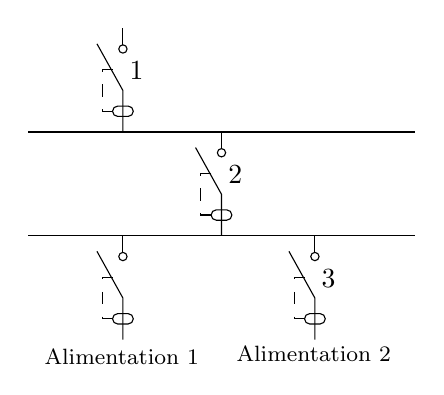
\begin{tikzpicture}[x=0.75pt,y=0.75pt,yscale=-1,xscale=1]
%uncomment if require: \path (0,218); %set diagram left start at 0, and has height of 218

%Straight Lines [id:da9017814347617055] 
\draw    (6.88,65) -- (193.13,65) ;
%Straight Lines [id:da9177255960935432] 
\draw    (40,22.5) -- (52.5,45) -- (52.5,65) ;
%Shape: Circle [id:dp6537007148868619] 
\draw   (54.5,25) .. controls (54.5,23.9) and (53.6,23) .. (52.5,23) .. controls (51.4,23) and (50.5,23.9) .. (50.5,25) .. controls (50.5,26.1) and (51.4,27) .. (52.5,27) .. controls (53.6,27) and (54.5,26.1) .. (54.5,25) -- cycle ;
%Straight Lines [id:da35199593727193423] 
\draw    (52.5,23) -- (52.5,15) ;
%Rounded Rect [id:dp6193458384304921] 
\draw   (47.5,55) .. controls (47.5,53.62) and (48.62,52.5) .. (50,52.5) -- (55,52.5) .. controls (56.38,52.5) and (57.5,53.62) .. (57.5,55) -- (57.5,55) .. controls (57.5,56.38) and (56.38,57.5) .. (55,57.5) -- (50,57.5) .. controls (48.62,57.5) and (47.5,56.38) .. (47.5,55) -- cycle ;
%Straight Lines [id:da9527186101720663] 
\draw  [dash pattern={on 4.5pt off 4.5pt}]  (47.5,35) -- (42.5,35) -- (42.5,55) -- (47.5,55) ;

%Straight Lines [id:da11508322768940726] 
\draw    (87.5,72.5) -- (100,95) -- (100,115) ;
%Shape: Circle [id:dp3391289042502843] 
\draw   (102,75) .. controls (102,73.9) and (101.1,73) .. (100,73) .. controls (98.9,73) and (98,73.9) .. (98,75) .. controls (98,76.1) and (98.9,77) .. (100,77) .. controls (101.1,77) and (102,76.1) .. (102,75) -- cycle ;
%Straight Lines [id:da23522970219666894] 
\draw    (100,73) -- (100,65) ;
%Rounded Rect [id:dp7801124199714764] 
\draw   (95,105) .. controls (95,103.62) and (96.12,102.5) .. (97.5,102.5) -- (102.5,102.5) .. controls (103.88,102.5) and (105,103.62) .. (105,105) -- (105,105) .. controls (105,106.38) and (103.88,107.5) .. (102.5,107.5) -- (97.5,107.5) .. controls (96.12,107.5) and (95,106.38) .. (95,105) -- cycle ;
%Straight Lines [id:da8144885809103521] 
\draw  [dash pattern={on 4.5pt off 4.5pt}]  (95,85) -- (90,85) -- (90,105) -- (95,105) ;

%Straight Lines [id:da5030372720493737] 
\draw    (40,122.5) -- (52.5,145) -- (52.5,165) ;
%Shape: Circle [id:dp6407081872243225] 
\draw   (54.5,125) .. controls (54.5,123.9) and (53.6,123) .. (52.5,123) .. controls (51.4,123) and (50.5,123.9) .. (50.5,125) .. controls (50.5,126.1) and (51.4,127) .. (52.5,127) .. controls (53.6,127) and (54.5,126.1) .. (54.5,125) -- cycle ;
%Straight Lines [id:da6460091175696209] 
\draw    (52.5,123) -- (52.5,115) ;
%Rounded Rect [id:dp9609968233337836] 
\draw   (47.5,155) .. controls (47.5,153.62) and (48.62,152.5) .. (50,152.5) -- (55,152.5) .. controls (56.38,152.5) and (57.5,153.62) .. (57.5,155) -- (57.5,155) .. controls (57.5,156.38) and (56.38,157.5) .. (55,157.5) -- (50,157.5) .. controls (48.62,157.5) and (47.5,156.38) .. (47.5,155) -- cycle ;
%Straight Lines [id:da6179641442257855] 
\draw  [dash pattern={on 4.5pt off 4.5pt}]  (47.5,135) -- (42.5,135) -- (42.5,155) -- (47.5,155) ;

%Straight Lines [id:da00291106623493409] 
\draw    (6.88,115) -- (193.13,115) ;
%Straight Lines [id:da11915371021246435] 
\draw    (132.5,122.5) -- (145,145) -- (145,165) ;
%Shape: Circle [id:dp1952488345903889] 
\draw   (147,125) .. controls (147,123.9) and (146.1,123) .. (145,123) .. controls (143.9,123) and (143,123.9) .. (143,125) .. controls (143,126.1) and (143.9,127) .. (145,127) .. controls (146.1,127) and (147,126.1) .. (147,125) -- cycle ;
%Straight Lines [id:da16332456687050667] 
\draw    (145,123) -- (145,115) ;
%Rounded Rect [id:dp31893341091728067] 
\draw   (140,155) .. controls (140,153.62) and (141.12,152.5) .. (142.5,152.5) -- (147.5,152.5) .. controls (148.88,152.5) and (150,153.62) .. (150,155) -- (150,155) .. controls (150,156.38) and (148.88,157.5) .. (147.5,157.5) -- (142.5,157.5) .. controls (141.12,157.5) and (140,156.38) .. (140,155) -- cycle ;
%Straight Lines [id:da8418511360368651] 
\draw  [dash pattern={on 4.5pt off 4.5pt}]  (140,135) -- (135,135) -- (135,155) -- (140,155) ;


% Text Node
\draw (13.5,168.5) node [anchor=north west][inner sep=0.75pt]   [align=left] {{\footnotesize Alimentation 1}};
% Text Node
\draw (106,167) node [anchor=north west][inner sep=0.75pt]   [align=left] {{\footnotesize Alimentation 2}};
% Text Node
\draw (54.5,30) node [anchor=north west][inner sep=0.75pt]   [align=left] {\Circled{1}};
% Text Node
\draw (102,80) node [anchor=north west][inner sep=0.75pt]   [align=left] {\Circled{2}};
% Text Node
\draw (147,130) node [anchor=north west][inner sep=0.75pt]   [align=left] {\Circled{3}};

\end{tikzpicture}
\subcaption{unifilaire de l'installation}
\end{subfigure}
\begin{subfigure}[b]{0.49\linewidth}
\centering
%--------------------------------------
%ELECTROTECHNIQUE - SCHEMA DE LIAISON A LA TERRE
%--------------------------------------

%utiliser les environnement \begin{comment} \end{comment} pour mettre en commentaire le préambule une fois la programmation appelée dans le document maître (!ne pas oublier de mettre en commentaire \end{document}!)

\begin{comment}

\documentclass[a4paper, 11pt, twoside, fleqn]{memoir}

\usepackage{AOCDTF}

%--------------------------------------
%CANEVAS
%--------------------------------------

\newcommand\BoxColor{\ifcase\thechapshift blue!30\or brown!30\or pink!30\or cyan!30\or green!30\or teal!30\or purple!30\or red!30\or olive!30\or orange!30\or lime!30\or gray!\or magenta!30\else yellow!30\fi} %définition de la couleur des marqueurs de chapitre

\newcounter{chapshift} %compteur de chapitre du marqueur de chapitre
\addtocounter{chapshift}{-1}
	
\newif\ifFrame %instruction conditionnelle pour les couleurs des pages
\Frametrue

\pagestyle{plain}

% the main command; the mandatory argument sets the color of the vertical box
\newcommand\ChapFrame{%
\AddEverypageHook{%
\ifFrame
\ifthenelse{\isodd{\value{page}}}
  {\backgroundsetup{contents={%
  \begin{tikzpicture}[overlay,remember picture]
  \node[
  	rounded corners=3pt,
    fill=\BoxColor,
    inner sep=0pt,
    rectangle,
    text width=1.5cm,
    text height=5.5cm,
    align=center,
    anchor=north west
  ] 
  at ($ (current page.north west) + (-0cm,-2*\thechapshift cm) $) %nombre négatif = espacement des marqueurs entre les différents chapitres (à régler en fin de rédaction) (4.5cm vaut un espacement équivalement à la hauteur du marqueur, une page peut en contenir 6 avec cet espacement-la mais il est le plus équilibré)
    {\rotatebox{90}{\hspace*{.5cm}%
      \parbox[c][1.2cm][t]{5cm}{%
        \raggedright\textcolor{black}{\sffamily\textbf{\leftmark}}}}};
  \end{tikzpicture}}}
  }
  {\backgroundsetup{contents={%
  \begin{tikzpicture}[overlay,remember picture]
  \node[
  	rounded corners=3pt,
    fill=\BoxColor,
    inner sep=0pt,
    rectangle,
    text width=1.5cm,
    text height=5.5cm,
    align=center,
    anchor=north east
  ] 
  at ($ (current page.north east) + (-0cm,-2*\thechapshift cm) $) %nombre négatif = espacement des marqueurs entre les différents chapitres (à régler en fin de rédaction) (4.5cm vaut un espacement équivalement à la hauteur du marqueur, une page peut en contenir 6 avec cet espacement-la mais il est le plus équilibré)
    {\rotatebox{90}{\hspace*{.5cm}%
      \parbox[c][1.2cm][t]{5cm}{%
        \raggedright\textcolor{black}{\sffamily\textbf{\leftmark}}}}};
  \end{tikzpicture}}}%
  }
  \BgMaterial%
  \fi%
}%
  \stepcounter{chapshift}
}

\renewcommand\chaptermark[1]{\markboth{\thechapter.~#1}{}} %redéfinition du marqueur de chapitre pour ne contenir que le titre du chapitre %à personnaliser selon le nombre de chapitre dans le cours

%--------------------------------------
%corps du document
%--------------------------------------

\begin{document} %corps du document
	\openleft %début de chapitre à gauche

\end{comment}

\begin{tikzpicture}
\begin{axis}[
/pgf/number format/.cd, use comma, 1000 sep={\,}, %format numérique européen
axis x line=bottom, axis y line = left,
no markers,
width=\linewidth, height=6cm, %hauteur/largeur
legend cell align={left}, legend style={at={(1,1.02)},anchor=south east},
grid=major,
grid=both,
enlarge x limits=false, 
xmode=log, xmin=10, xmax=12000, xtick={10, 100, 1000, 10000},
xlabel style={text width=\linewidth}, ylabel style={text width=5cm},
xlabel={Intensité du courant de fonctionnement résiduels assignés en \si{\milli\ampere}}, log ticks with fixed point,
ymode=log, ymin=10, ymax=13000, ytick={10, 100, 1000, 10000},
ylabel={Durée $t$ du passage du courant en \si{\milli\second}},
]


\path[name path=gbi] (14.517932133997183,10000) -- (14.517932133997183,10) -- (10000,10);
\path[name path=hdi] (29.60932939627084,10000) -- (29.60932939627084,352.7323205216774) -- (146.77992676220705,40.34961693676772) -- (10000,40.34961693676772);
\addplot [blue, opacity=0.5] fill between[of=gbi and hdi];
\addlegendentry{Instantané \circrefseul{pas:40}};

\path[name path=gbs] (10000,40.34961693676772) -- (2682.6957952797275,40.34961693676772) -- (1973.504382868977,48.54353364246499) -- (704.075200660645,60.39790821830388) -- (289.6708287824031,149.68644761350285) -- (150,502.0302968341689
) -- (150,10000);
\path[name path=hds] (10000,149.68644761350285) -- (1435.9617019622142,149.68644761350285) -- (590.7837911587943,213.04294320497598) -- (590.7837911587943,213.04294320497598) -- (299.357729472049,502.0302968341689
) -- (299.357729472049,10000);
\addplot [red, opacity=0.5] fill between[of=gbs and hds];
\addlegendentry{Sélectif \circrefseul{pas:41}};

\path[name path=gbr] (10000,150) -- (1655.9515234819182,150) -- (474.45002755086585,502.0302968341689) -- (474.45002755086585,10000);
\path[name path=hdr] (10000,313.5814507256924) -- (4796.808502304898,313.5814507256924) -- (1033.441063880556,919.3982010218539) -- (1033.441063880556,10000);
\addplot  [brown, opacity=0.5]  fill between[of=gbr and hdr];
\addlegendentry{Retardé \circrefseul{pas:42}};

\addplot (14.517932133997183,10000) -- (14.517932133997183,10) -- (10000,10) -- (10000,40.34961693676772) -- (146.77992676220705,40.34961693676772) -- (29.60932939627084,352.7323205216774) -- (29.60932939627084,10000) -- cycle;
\addplot [red] (10000,40.34961693676772) -- (2682.6957952797275,40.34961693676772) -- (1973.504382868977,48.54353364246499) -- (704.075200660645,60.39790821830388) -- (289.6708287824031,149.68644761350285) -- (150,502.0302968341689
) -- (150,10000) -- (299.357729472049,10000) -- (299.357729472049,502.0302968341689
) -- (590.7837911587943,213.04294320497598) -- (590.7837911587943,213.04294320497598)  -- (1435.9617019622142,149.68644761350285) -- (10000,149.68644761350285) -- cycle;
\addplot [brown] (10000,150) -- (1655.9515234819182,150) -- (474.45002755086585,502.0302968341689) -- (474.45002755086585,10000) -- (1033.441063880556,10000) -- (1033.441063880556,919.3982010218539) -- (4796.808502304898,313.5814507256924) -- (10000,313.5814507256924) -- cycle;

\end{axis}
\end{tikzpicture}





%\end{document}


\subcaption{courbe des courants de fonctionnement résiduels assignés en fonction du temps\supercite{Schneider:coordinationDDR}}
\end{subfigure}
\end{figure}

\paragraph{Cas particulier de coordination avec les DDR de type B}

\begin{wrapfigure}{R}{0pt}
\ffigbox[\FBwidth]
{\caption{Cas d'une sélectivité à deux niveaux entre des DDR de type B\label{fig:selectivite_DDR_type_B}}}
{\tikzset{every picture/.style={line width=0.75pt}} %set default line width to 0.75pt        

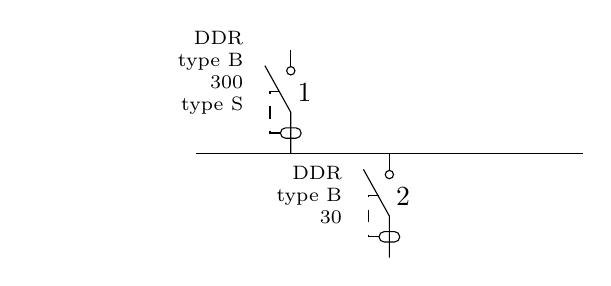
\begin{tikzpicture}[x=0.75pt,y=0.75pt,yscale=-1,xscale=1]
%uncomment if require: \path (0,138); %set diagram left start at 0, and has height of 138

%Straight Lines [id:da8169631390975441] 
\draw    (119.38,65) -- (305.63,65) ;
%Straight Lines [id:da4319979510089893] 
\draw    (152.5,22.5) -- (165,45) -- (165,65) ;
%Shape: Circle [id:dp7461171752369792] 
\draw   (167,25) .. controls (167,23.9) and (166.1,23) .. (165,23) .. controls (163.9,23) and (163,23.9) .. (163,25) .. controls (163,26.1) and (163.9,27) .. (165,27) .. controls (166.1,27) and (167,26.1) .. (167,25) -- cycle ;
%Straight Lines [id:da8451811097550901] 
\draw    (165,23) -- (165,15) ;
%Rounded Rect [id:dp18053555138635746] 
\draw   (160,55) .. controls (160,53.62) and (161.12,52.5) .. (162.5,52.5) -- (167.5,52.5) .. controls (168.88,52.5) and (170,53.62) .. (170,55) -- (170,55) .. controls (170,56.38) and (168.88,57.5) .. (167.5,57.5) -- (162.5,57.5) .. controls (161.12,57.5) and (160,56.38) .. (160,55) -- cycle ;
%Straight Lines [id:da08951652624873063] 
\draw  [dash pattern={on 4.5pt off 4.5pt}]  (160,35) -- (155,35) -- (155,55) -- (160,55) ;

%Straight Lines [id:da7410030620837423] 
\draw    (200,72.5) -- (212.5,95) -- (212.5,115) ;
%Shape: Circle [id:dp05670563209773016] 
\draw   (214.5,75) .. controls (214.5,73.9) and (213.6,73) .. (212.5,73) .. controls (211.4,73) and (210.5,73.9) .. (210.5,75) .. controls (210.5,76.1) and (211.4,77) .. (212.5,77) .. controls (213.6,77) and (214.5,76.1) .. (214.5,75) -- cycle ;
%Straight Lines [id:da816027499463629] 
\draw    (212.5,73) -- (212.5,65) ;
%Rounded Rect [id:dp3947599360896624] 
\draw   (207.5,105) .. controls (207.5,103.62) and (208.62,102.5) .. (210,102.5) -- (215,102.5) .. controls (216.38,102.5) and (217.5,103.62) .. (217.5,105) -- (217.5,105) .. controls (217.5,106.38) and (216.38,107.5) .. (215,107.5) -- (210,107.5) .. controls (208.62,107.5) and (207.5,106.38) .. (207.5,105) -- cycle ;
%Straight Lines [id:da6953851857801584] 
\draw  [dash pattern={on 4.5pt off 4.5pt}]  (207.5,85) -- (202.5,85) -- (202.5,105) -- (207.5,105) ;


% Text Node
\draw (167,30) node [anchor=north west][inner sep=0.75pt]   [align=left] {\Circled{1}};
% Text Node
\draw (214.5,80) node [anchor=north west][inner sep=0.75pt]   [align=left] {\Circled{2}};
% Text Node
\draw (38.5,4.5) node [anchor=north west][inner sep=0.75pt]  [font=\scriptsize] [align=left] {\begin{minipage}[lt]{76.744375pt}\setlength\topsep{0pt}
\begin{flushright}
DDR\\
type B\\
\SI{300}{\milli\ampere}\\
type S
\end{flushright}

\end{minipage}};
% Text Node
\draw (86,69.5) node [anchor=north west][inner sep=0.75pt]  [font=\scriptsize] [align=left] {\begin{minipage}[lt]{76.744375pt}\setlength\topsep{0pt}
\begin{flushright}
DDR\\
type B\\
\SI{30}{\milli\ampere}
\end{flushright}

\end{minipage}};
\end{tikzpicture}}
\end{wrapfigure}

En présence d'un courant de fuite à la terre possible en courant continu (typiquement le cas pour les chargeurs de voiture), un DDR de type B doit être utilisé pour la protection contre les contacts indirects. Dans ce cas, le DDR en amont ne doit pas être aveuglé par le courant résiduel continu possible et doit assurer sa protection normale lorsqu'un courant de défaut apparait dans une autre partie de l'installation.\\
Par exemple, dans le schéma en \superref{fig:selectivite_DDR_type_B}, le DDR $I_{\Delta n} = \SI{30}{\milli\ampere}$ de type B au niveau 2 peut avoir un seuil de déclenchement courant continu maximum de $2 \times I_{\Delta n}$, selon la norme produit DDR CEI 62423\supercite{IEC:62423-2009}. Cela signifie que ce DDR de $I_{\Delta n} = \SI{30}{\milli\ampere}$ de type B pourrait laisser passer un courant résiduel de presque \SI{60}{\milli\ampere} $\mathdirectcurrent$ sans déclenchement et que le DDR en amont ne devrait perdre aucune de ses performances avec la présence de ce niveau élevé de courant résiduel $mathdirectcurrent$. C'est pourquoi il est souvent proposé d'utiliser un DDR de type B au niveau 1 pour éviter tout effet d'aveuglement par le courant continu.\\

Toutefois, certains constructeurs implémentent dans leurs DDR de type A la capacité de ne pas être sensibles au courant résiduel $\mathdirectcurrent$ en dessous d'un certain seuil de courant de défaut ($\SI{60}{\milli\ampere}$ pour la marque Schneider\supercite{Schneider:coordinationDDR}). Cela permet d'éviter la pose d'un DDR de type B en amont, plus coûteux qu'un DDR de type A, tout en conservant les capacités de détection des DDR de types A et AC.

\subsection{Mise à la terre des appareils et structures conductrices}

\subsubsection{Mise à la terre des appareils électriques}

Les appareils de classe d'isolation I doivent être raccordées à des prises 2P + T \Circled{1} au moyen de fiches 2P + T \Circled{2}. Ces prises équipent maintenant tous les logements dont l'installation respecte la norme NF C15-100. Si ces appareils ne présentent pas de fiches, elles sont raccordées au moyen de boitiers d'encastrements appropriés.\\
Sont particulièrement concernés par cette connexion vers la terre les appareils combinant électricité et eau (lave-vaisselle, lave-linge, cafetière\ldots \Circled{3}). Les fuites d'eau peuvent effectivement  provoquer relativement facilement la mise sous tension de la carcasse métallique de l'appareil.

\subsubsection{Liaison équipotentielle}

Pour protéger les biens et les personnes des contacts indirects, en plus de connecter toutes les carcasses métalliques des appareils de classe d'isolation II vers la terre, il convient de connecter toutes les structures métalliques du bâtiment susceptibles d'être en contact avec un individu \emph{et} d'être mise sous tension accidentellement. Sont concernés par la mise à la terre \Circled{4} :
\begin{itemize}
\item tuyauterie (même non conductrice car l'eau y transitant l'est)\,;
\item baignoire et bac de douche (fonte, métal\ldots)\,;
\item charpente métallique\,;
\item autres structures métalliques (pouvant varier selon les exigences de sécurité).
\end{itemize}
Cette connexion, effectuée par un \emph{conducteur de protection} PE \Circled{5} (obligatoirement en jaune-vert), de toutes les structures conductrices et appareils de classe I constitue la \emph{liaison équipotentielle}. Tous ces conducteurs sont connectés sur une \emph{barrette de terre} \Circled{8} dans le Tableau Général Basse Tension (TGBT) et sont séparés de la \emph{prise de terre de l'installation électrique} \Circled{9} par une \emph{barrette de mesure} \Circled{10} (dénommé également \emph{couteau de terre}).\\

Afin d'assurer la meilleure protection possible, les conducteurs de protection doivent présenter une section de câble et des raccordements dimensionnés à même de garantir une résistance de la liaison équipotentielle d'une valeur inférieure à \SI{2}{\ohm}. Cette résistance est contrôlée au moyen d'un \emph{testeur de continuité} spécifique.
\begin{table}[H]
\caption{Section des conducteurs de protection}
\begin{tabularx}{\linewidth}{c X p{5,5cm}}
\toprule
\thead{Schéma}		& \thead{Type de conducteur}		& \thead{Section} \\
\midrule
\Circled{5} 		& Conducteur de protection transitant dans la même canalisation que les phase(s) et neutre		& identique à celle des phase(s) et neutre \\
\addlinespace
	&		Conducteur de protection protégé mécaniquement																	& \SI{2,5}{\square\milli\meter} \\
\addlinespace
	&		Conducteur de protection non protégé mécaniquement															& \SI{4}{\square\milli\meter} \\
\addlinespace
\Circled{6}		&	Conducteur principal de protection																							& \SI{16}{\square\milli\meter} en cuivre isolé \\
\addlinespace
\Circled{7} 		& Conducteur de terre																												& 
\begin{tabdescription}
\item[Selon les caractéristiques :]\hfill
\begin{compactitemize}
\item \SI{16}{\square\milli\meter} en cuivre isolé\,;
\item \SI{25}{\square\milli\meter} en cuivre nu\,;
\item \SI{50}{\square\milli\meter} en aluminium ou en fer.
\end{compactitemize} 
\end{tabdescription}
\\
\bottomrule
\end{tabularx}
\end{table}

%--------------------------------------
%ELECTROTECHNIQUE - SCHEMA DE LIAISON A LA TERRE
%--------------------------------------

%utiliser les environnement \begin{comment} \end{comment} pour mettre en commentaire le préambule une fois la programmation appelée dans le document maître (!ne pas oublier de mettre en commentaire \end{document}!)

\begin{comment}

\documentclass[a4paper, 11pt, twoside, fleqn]{memoir}

\usepackage{AOCDTF}

\marqueurchapitre

%lien d'édition des figures Tikz sur le site mathcha.io (rajouter le lien d'une modification effectuée sur la figure tikz avec le nom du modificateur car il n'y a qu'un lien par compte)

%lien mathcha Bruno Douchy : https://www.mathcha.io/editor/O4QxWcpXSQqTxP7Mz4Cv2xzVJI80LNjskrPYpv

%--------------------------------------
%corps du document
%--------------------------------------

\begin{document} %corps du document
	\openleft %début de chapitre à gauche

\end{comment}


\begin{figure}
\caption{Liaison équipotentielle}


\tikzset{every picture/.style={line width=0.75pt}} %set default line width to 0.75pt        

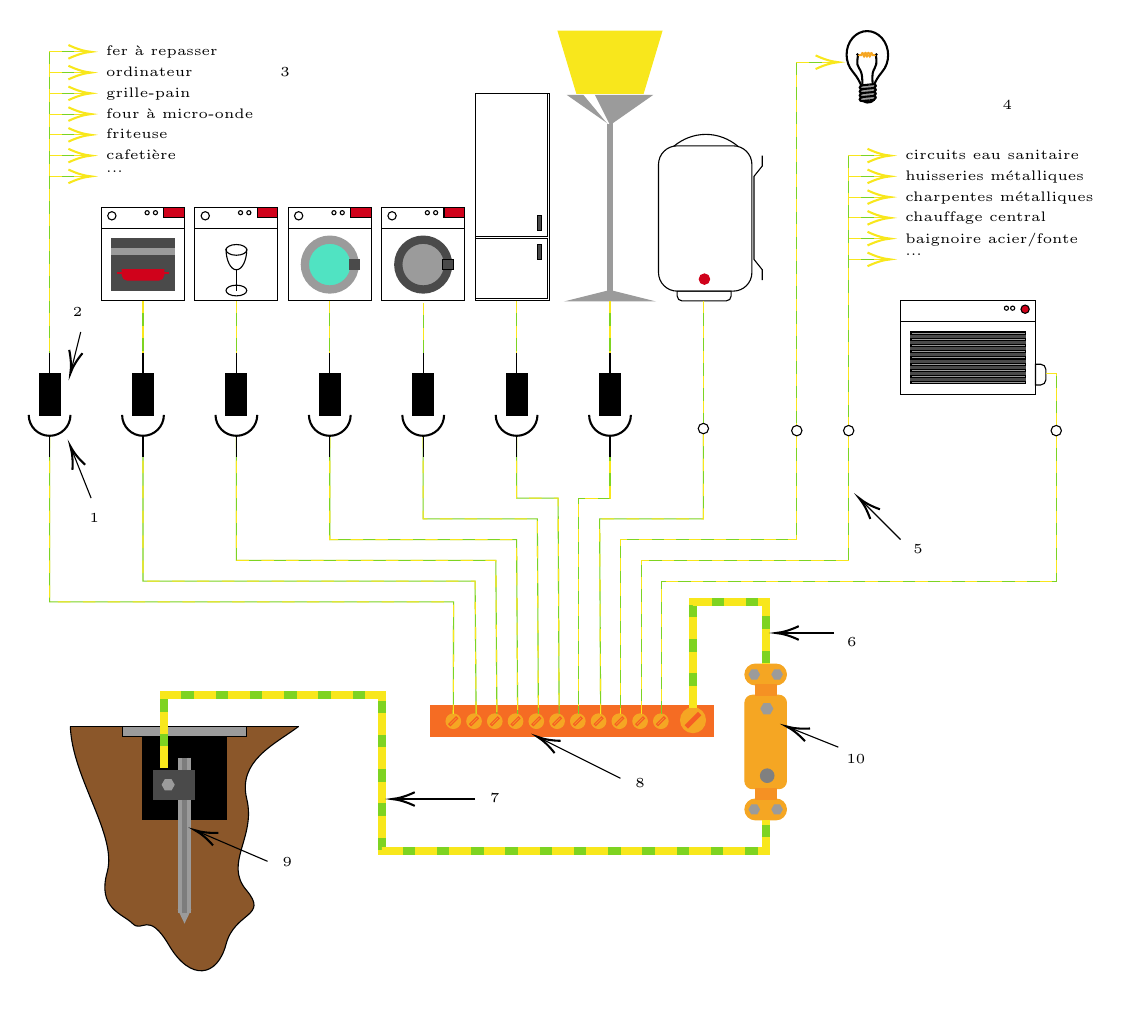
\begin{tikzpicture}[x=0.75pt,y=0.75pt,yscale=-1,xscale=1]
%uncomment if require: \path (0,484); %set diagram left start at 0, and has height of 484

%Shape: Rectangle [id:dp12779471624214456] 
\draw  [color={rgb, 255:red, 245; green, 108; blue, 35 }  ,draw opacity=1 ][fill={rgb, 255:red, 245; green, 108; blue, 35 }  ,fill opacity=1 ] (203.5,349.9) -- (340,349.9) -- (340,365) -- (203.5,365) -- cycle ;
%Shape: Circle [id:dp3978776166680479] 
\draw  [color={rgb, 255:red, 245; green, 166; blue, 35 }  ,draw opacity=1 ][fill={rgb, 255:red, 245; green, 166; blue, 35 }  ,fill opacity=1 ] (211,357.5) .. controls (211,355.57) and (212.57,354) .. (214.5,354) .. controls (216.43,354) and (218,355.57) .. (218,357.5) .. controls (218,359.43) and (216.43,361) .. (214.5,361) .. controls (212.57,361) and (211,359.43) .. (211,357.5) -- cycle ;
%Shape: Rectangle [id:dp5513162261841694] 
\draw  [color={rgb, 255:red, 245; green, 94; blue, 35 }  ,draw opacity=1 ][fill={rgb, 255:red, 245; green, 166; blue, 35 }  ,fill opacity=1 ] (215.91,355.38) -- (216.62,356.09) -- (213.09,359.62) -- (212.38,358.91) -- cycle ;

%Shape: Circle [id:dp990223085537162] 
\draw  [color={rgb, 255:red, 245; green, 166; blue, 35 }  ,draw opacity=1 ][fill={rgb, 255:red, 245; green, 166; blue, 35 }  ,fill opacity=1 ] (221,357.5) .. controls (221,355.57) and (222.57,354) .. (224.5,354) .. controls (226.43,354) and (228,355.57) .. (228,357.5) .. controls (228,359.43) and (226.43,361) .. (224.5,361) .. controls (222.57,361) and (221,359.43) .. (221,357.5) -- cycle ;
%Shape: Rectangle [id:dp7901194427174768] 
\draw  [color={rgb, 255:red, 245; green, 94; blue, 35 }  ,draw opacity=1 ][fill={rgb, 255:red, 245; green, 166; blue, 35 }  ,fill opacity=1 ] (225.91,355.38) -- (226.62,356.09) -- (223.09,359.62) -- (222.38,358.91) -- cycle ;

%Shape: Circle [id:dp23561107154810057] 
\draw  [color={rgb, 255:red, 245; green, 166; blue, 35 }  ,draw opacity=1 ][fill={rgb, 255:red, 245; green, 166; blue, 35 }  ,fill opacity=1 ] (231,357.5) .. controls (231,355.57) and (232.57,354) .. (234.5,354) .. controls (236.43,354) and (238,355.57) .. (238,357.5) .. controls (238,359.43) and (236.43,361) .. (234.5,361) .. controls (232.57,361) and (231,359.43) .. (231,357.5) -- cycle ;
%Shape: Rectangle [id:dp2645964583580035] 
\draw  [color={rgb, 255:red, 245; green, 94; blue, 35 }  ,draw opacity=1 ][fill={rgb, 255:red, 245; green, 166; blue, 35 }  ,fill opacity=1 ] (235.91,355.38) -- (236.62,356.09) -- (233.09,359.62) -- (232.38,358.91) -- cycle ;

%Shape: Circle [id:dp004074096804411842] 
\draw  [color={rgb, 255:red, 245; green, 166; blue, 35 }  ,draw opacity=1 ][fill={rgb, 255:red, 245; green, 166; blue, 35 }  ,fill opacity=1 ] (241,357.5) .. controls (241,355.57) and (242.57,354) .. (244.5,354) .. controls (246.43,354) and (248,355.57) .. (248,357.5) .. controls (248,359.43) and (246.43,361) .. (244.5,361) .. controls (242.57,361) and (241,359.43) .. (241,357.5) -- cycle ;
%Shape: Rectangle [id:dp15563792683915179] 
\draw  [color={rgb, 255:red, 245; green, 94; blue, 35 }  ,draw opacity=1 ][fill={rgb, 255:red, 245; green, 166; blue, 35 }  ,fill opacity=1 ] (245.91,355.38) -- (246.62,356.09) -- (243.09,359.62) -- (242.38,358.91) -- cycle ;

%Shape: Circle [id:dp42723031236585807] 
\draw  [color={rgb, 255:red, 245; green, 166; blue, 35 }  ,draw opacity=1 ][fill={rgb, 255:red, 245; green, 166; blue, 35 }  ,fill opacity=1 ] (251,357.5) .. controls (251,355.57) and (252.57,354) .. (254.5,354) .. controls (256.43,354) and (258,355.57) .. (258,357.5) .. controls (258,359.43) and (256.43,361) .. (254.5,361) .. controls (252.57,361) and (251,359.43) .. (251,357.5) -- cycle ;
%Shape: Rectangle [id:dp23601803414152545] 
\draw  [color={rgb, 255:red, 245; green, 94; blue, 35 }  ,draw opacity=1 ][fill={rgb, 255:red, 245; green, 166; blue, 35 }  ,fill opacity=1 ] (255.91,355.38) -- (256.62,356.09) -- (253.09,359.62) -- (252.38,358.91) -- cycle ;

%Shape: Circle [id:dp21722774235746978] 
\draw  [color={rgb, 255:red, 245; green, 166; blue, 35 }  ,draw opacity=1 ][fill={rgb, 255:red, 245; green, 166; blue, 35 }  ,fill opacity=1 ] (261,357.5) .. controls (261,355.57) and (262.57,354) .. (264.5,354) .. controls (266.43,354) and (268,355.57) .. (268,357.5) .. controls (268,359.43) and (266.43,361) .. (264.5,361) .. controls (262.57,361) and (261,359.43) .. (261,357.5) -- cycle ;
%Shape: Rectangle [id:dp3473865244123996] 
\draw  [color={rgb, 255:red, 245; green, 94; blue, 35 }  ,draw opacity=1 ][fill={rgb, 255:red, 245; green, 166; blue, 35 }  ,fill opacity=1 ] (265.91,355.38) -- (266.62,356.09) -- (263.09,359.62) -- (262.38,358.91) -- cycle ;

%Shape: Circle [id:dp43806185211532767] 
\draw  [color={rgb, 255:red, 245; green, 166; blue, 35 }  ,draw opacity=1 ][fill={rgb, 255:red, 245; green, 166; blue, 35 }  ,fill opacity=1 ] (271,357.5) .. controls (271,355.57) and (272.57,354) .. (274.5,354) .. controls (276.43,354) and (278,355.57) .. (278,357.5) .. controls (278,359.43) and (276.43,361) .. (274.5,361) .. controls (272.57,361) and (271,359.43) .. (271,357.5) -- cycle ;
%Shape: Rectangle [id:dp47605810022702744] 
\draw  [color={rgb, 255:red, 245; green, 94; blue, 35 }  ,draw opacity=1 ][fill={rgb, 255:red, 245; green, 166; blue, 35 }  ,fill opacity=1 ] (275.91,355.38) -- (276.62,356.09) -- (273.09,359.62) -- (272.38,358.91) -- cycle ;

%Shape: Circle [id:dp12453339823990162] 
\draw  [color={rgb, 255:red, 245; green, 166; blue, 35 }  ,draw opacity=1 ][fill={rgb, 255:red, 245; green, 166; blue, 35 }  ,fill opacity=1 ] (281,357.5) .. controls (281,355.57) and (282.57,354) .. (284.5,354) .. controls (286.43,354) and (288,355.57) .. (288,357.5) .. controls (288,359.43) and (286.43,361) .. (284.5,361) .. controls (282.57,361) and (281,359.43) .. (281,357.5) -- cycle ;
%Shape: Rectangle [id:dp6051367753026781] 
\draw  [color={rgb, 255:red, 245; green, 94; blue, 35 }  ,draw opacity=1 ][fill={rgb, 255:red, 245; green, 166; blue, 35 }  ,fill opacity=1 ] (285.91,355.38) -- (286.62,356.09) -- (283.09,359.62) -- (282.38,358.91) -- cycle ;

%Shape: Circle [id:dp7759537392826514] 
\draw  [color={rgb, 255:red, 245; green, 166; blue, 35 }  ,draw opacity=1 ][fill={rgb, 255:red, 245; green, 166; blue, 35 }  ,fill opacity=1 ] (291,357.5) .. controls (291,355.57) and (292.57,354) .. (294.5,354) .. controls (296.43,354) and (298,355.57) .. (298,357.5) .. controls (298,359.43) and (296.43,361) .. (294.5,361) .. controls (292.57,361) and (291,359.43) .. (291,357.5) -- cycle ;
%Shape: Rectangle [id:dp917105554714615] 
\draw  [color={rgb, 255:red, 245; green, 94; blue, 35 }  ,draw opacity=1 ][fill={rgb, 255:red, 245; green, 166; blue, 35 }  ,fill opacity=1 ] (295.91,355.38) -- (296.62,356.09) -- (293.09,359.62) -- (292.38,358.91) -- cycle ;

%Shape: Circle [id:dp02780975411771036] 
\draw  [color={rgb, 255:red, 245; green, 166; blue, 35 }  ,draw opacity=1 ][fill={rgb, 255:red, 245; green, 166; blue, 35 }  ,fill opacity=1 ] (301,357.5) .. controls (301,355.57) and (302.57,354) .. (304.5,354) .. controls (306.43,354) and (308,355.57) .. (308,357.5) .. controls (308,359.43) and (306.43,361) .. (304.5,361) .. controls (302.57,361) and (301,359.43) .. (301,357.5) -- cycle ;
%Shape: Rectangle [id:dp33128134488839245] 
\draw  [color={rgb, 255:red, 245; green, 94; blue, 35 }  ,draw opacity=1 ][fill={rgb, 255:red, 245; green, 166; blue, 35 }  ,fill opacity=1 ] (305.91,355.38) -- (306.62,356.09) -- (303.09,359.62) -- (302.38,358.91) -- cycle ;

%Shape: Circle [id:dp24766499702501743] 
\draw  [color={rgb, 255:red, 245; green, 166; blue, 35 }  ,draw opacity=1 ][fill={rgb, 255:red, 245; green, 166; blue, 35 }  ,fill opacity=1 ] (311,357.5) .. controls (311,355.57) and (312.57,354) .. (314.5,354) .. controls (316.43,354) and (318,355.57) .. (318,357.5) .. controls (318,359.43) and (316.43,361) .. (314.5,361) .. controls (312.57,361) and (311,359.43) .. (311,357.5) -- cycle ;
%Shape: Rectangle [id:dp9353732861352104] 
\draw  [color={rgb, 255:red, 245; green, 94; blue, 35 }  ,draw opacity=1 ][fill={rgb, 255:red, 245; green, 166; blue, 35 }  ,fill opacity=1 ] (315.91,355.38) -- (316.62,356.09) -- (313.09,359.62) -- (312.38,358.91) -- cycle ;

%Shape: Circle [id:dp37341465274388497] 
\draw  [color={rgb, 255:red, 245; green, 166; blue, 35 }  ,draw opacity=1 ][fill={rgb, 255:red, 245; green, 166; blue, 35 }  ,fill opacity=1 ] (324,357) .. controls (324,353.69) and (326.69,351) .. (330,351) .. controls (333.31,351) and (336,353.69) .. (336,357) .. controls (336,360.31) and (333.31,363) .. (330,363) .. controls (326.69,363) and (324,360.31) .. (324,357) -- cycle ;
%Shape: Rectangle [id:dp9630557822680567] 
\draw  [color={rgb, 255:red, 245; green, 94; blue, 35 }  ,draw opacity=1 ][fill={rgb, 255:red, 245; green, 94; blue, 35 }  ,fill opacity=1 ] (332.42,353.36) -- (333.64,354.58) -- (327.58,360.64) -- (326.36,359.42) -- cycle ;

%Straight Lines [id:da24513459081521916] 
\draw [color={rgb, 255:red, 126; green, 211; blue, 33 }  ,draw opacity=1 ]   (20,220) -- (20,300) -- (214.66,300) -- (214.5,354) ;
%Straight Lines [id:da4596588122450417] 
\draw [color={rgb, 255:red, 248; green, 231; blue, 28 }  ,draw opacity=1 ] [dash pattern={on 4.5pt off 4.5pt}]  (20,220) -- (20,300) -- (214.66,300) -- (214.5,354) ;
%Straight Lines [id:da7477140703123141] 
\draw [color={rgb, 255:red, 126; green, 211; blue, 33 }  ,draw opacity=1 ]   (35,35) -- (20,35) -- (20,190) ;
%Straight Lines [id:da3286874762261832] 
\draw [color={rgb, 255:red, 248; green, 231; blue, 28 }  ,draw opacity=1 ] [dash pattern={on 4.5pt off 4.5pt}]  (38,35) -- (20,35) -- (20,190) ;
\draw [shift={(40,35)}, rotate = 180] [color={rgb, 255:red, 248; green, 231; blue, 28 }  ,draw opacity=1 ][line width=0.75]    (10.93,-3.29) .. controls (6.95,-1.4) and (3.31,-0.3) .. (0,0) .. controls (3.31,0.3) and (6.95,1.4) .. (10.93,3.29)   ;

%Straight Lines [id:da4598837213780632] 
\draw [color={rgb, 255:red, 126; green, 211; blue, 33 }  ,draw opacity=1 ]   (35,45) -- (20,45) ;
%Straight Lines [id:da839734818655239] 
\draw [color={rgb, 255:red, 248; green, 231; blue, 28 }  ,draw opacity=1 ] [dash pattern={on 4.5pt off 4.5pt}]  (38,45) -- (20,45) ;
\draw [shift={(40,45)}, rotate = 180] [color={rgb, 255:red, 248; green, 231; blue, 28 }  ,draw opacity=1 ][line width=0.75]    (10.93,-3.29) .. controls (6.95,-1.4) and (3.31,-0.3) .. (0,0) .. controls (3.31,0.3) and (6.95,1.4) .. (10.93,3.29)   ;

%Straight Lines [id:da09587209918948914] 
\draw [color={rgb, 255:red, 126; green, 211; blue, 33 }  ,draw opacity=1 ]   (35,55) -- (20,55) ;
%Straight Lines [id:da9944741609170024] 
\draw [color={rgb, 255:red, 248; green, 231; blue, 28 }  ,draw opacity=1 ] [dash pattern={on 4.5pt off 4.5pt}]  (38,55) -- (20,55) ;
\draw [shift={(40,55)}, rotate = 180] [color={rgb, 255:red, 248; green, 231; blue, 28 }  ,draw opacity=1 ][line width=0.75]    (10.93,-3.29) .. controls (6.95,-1.4) and (3.31,-0.3) .. (0,0) .. controls (3.31,0.3) and (6.95,1.4) .. (10.93,3.29)   ;

%Straight Lines [id:da7884693135725294] 
\draw [color={rgb, 255:red, 126; green, 211; blue, 33 }  ,draw opacity=1 ]   (35,65) -- (20,65) ;
%Straight Lines [id:da239241815637814] 
\draw [color={rgb, 255:red, 248; green, 231; blue, 28 }  ,draw opacity=1 ] [dash pattern={on 4.5pt off 4.5pt}]  (38,65) -- (20,65) ;
\draw [shift={(40,65)}, rotate = 180] [color={rgb, 255:red, 248; green, 231; blue, 28 }  ,draw opacity=1 ][line width=0.75]    (10.93,-3.29) .. controls (6.95,-1.4) and (3.31,-0.3) .. (0,0) .. controls (3.31,0.3) and (6.95,1.4) .. (10.93,3.29)   ;

%Straight Lines [id:da8880878687374321] 
\draw [color={rgb, 255:red, 126; green, 211; blue, 33 }  ,draw opacity=1 ]   (35,75) -- (20,75) ;
%Straight Lines [id:da43421080173788573] 
\draw [color={rgb, 255:red, 248; green, 231; blue, 28 }  ,draw opacity=1 ] [dash pattern={on 4.5pt off 4.5pt}]  (38,75) -- (20,75) ;
\draw [shift={(40,75)}, rotate = 180] [color={rgb, 255:red, 248; green, 231; blue, 28 }  ,draw opacity=1 ][line width=0.75]    (10.93,-3.29) .. controls (6.95,-1.4) and (3.31,-0.3) .. (0,0) .. controls (3.31,0.3) and (6.95,1.4) .. (10.93,3.29)   ;

%Straight Lines [id:da4265288409692696] 
\draw [color={rgb, 255:red, 126; green, 211; blue, 33 }  ,draw opacity=1 ]   (35,85) -- (20,85) ;
%Straight Lines [id:da09693100530986232] 
\draw [color={rgb, 255:red, 248; green, 231; blue, 28 }  ,draw opacity=1 ] [dash pattern={on 4.5pt off 4.5pt}]  (38,85) -- (20,85) ;
\draw [shift={(40,85)}, rotate = 180] [color={rgb, 255:red, 248; green, 231; blue, 28 }  ,draw opacity=1 ][line width=0.75]    (10.93,-3.29) .. controls (6.95,-1.4) and (3.31,-0.3) .. (0,0) .. controls (3.31,0.3) and (6.95,1.4) .. (10.93,3.29)   ;

%Straight Lines [id:da18824193936949507] 
\draw [color={rgb, 255:red, 126; green, 211; blue, 33 }  ,draw opacity=1 ]   (35,95) -- (20,95) ;
%Straight Lines [id:da8037918831525122] 
\draw [color={rgb, 255:red, 248; green, 231; blue, 28 }  ,draw opacity=1 ] [dash pattern={on 4.5pt off 4.5pt}]  (38,95) -- (20,95) ;
\draw [shift={(40,95)}, rotate = 180] [color={rgb, 255:red, 248; green, 231; blue, 28 }  ,draw opacity=1 ][line width=0.75]    (10.93,-3.29) .. controls (6.95,-1.4) and (3.31,-0.3) .. (0,0) .. controls (3.31,0.3) and (6.95,1.4) .. (10.93,3.29)   ;

%Straight Lines [id:da7880540826459623] 
\draw [color={rgb, 255:red, 126; green, 211; blue, 33 }  ,draw opacity=1 ]   (65,220) -- (65,290) -- (225,290) -- (225.5,354) ;
%Straight Lines [id:da8587552191330365] 
\draw [color={rgb, 255:red, 248; green, 231; blue, 28 }  ,draw opacity=1 ] [dash pattern={on 4.5pt off 4.5pt}]  (65,220) -- (65,290) -- (159.78,290) -- (225,290) -- (225.5,354) ;
%Straight Lines [id:da6477628826976815] 
\draw [color={rgb, 255:red, 126; green, 211; blue, 33 }  ,draw opacity=1 ]   (65,155) -- (65,155) -- (65,190) ;
%Straight Lines [id:da2838867143416234] 
\draw [color={rgb, 255:red, 248; green, 231; blue, 28 }  ,draw opacity=1 ] [dash pattern={on 4.5pt off 4.5pt}]  (65,155) -- (65,190) ;
%Shape: Rectangle [id:dp04022794256338735] 
\draw   (135,110) -- (175,110) -- (175,155) -- (135,155) -- cycle ;
%Shape: Circle [id:dp7114048760384077] 
\draw  [color={rgb, 255:red, 155; green, 155; blue, 155 }  ,draw opacity=1 ][fill={rgb, 255:red, 80; green, 227; blue, 194 }  ,fill opacity=1 ][line width=3]  (143,137.5) .. controls (143,130.87) and (148.37,125.5) .. (155,125.5) .. controls (161.63,125.5) and (167,130.87) .. (167,137.5) .. controls (167,144.13) and (161.63,149.5) .. (155,149.5) .. controls (148.37,149.5) and (143,144.13) .. (143,137.5) -- cycle ;
%Shape: Rectangle [id:dp24112973693492956] 
\draw  [color={rgb, 255:red, 74; green, 74; blue, 74 }  ,draw opacity=1 ][fill={rgb, 255:red, 74; green, 74; blue, 74 }  ,fill opacity=1 ] (164.5,134.92) -- (169.5,134.92) -- (169.5,140.08) -- (164.5,140.08) -- cycle ;
%Shape: Rectangle [id:dp6934540976609278] 
\draw   (135,110) -- (175,110) -- (175,120) -- (135,120) -- cycle ;
%Shape: Rectangle [id:dp676606923437384] 
\draw  [color={rgb, 255:red, 0; green, 0; blue, 0 }  ,draw opacity=1 ][fill={rgb, 255:red, 208; green, 2; blue, 27 }  ,fill opacity=1 ] (165,110) -- (175,110) -- (175,115) -- (165,115) -- cycle ;
%Shape: Circle [id:dp51451854322091] 
\draw   (162,112.5) .. controls (162,111.95) and (161.55,111.5) .. (161,111.5) .. controls (160.45,111.5) and (160,111.95) .. (160,112.5) .. controls (160,113.05) and (160.45,113.5) .. (161,113.5) .. controls (161.55,113.5) and (162,113.05) .. (162,112.5) -- cycle ;
%Shape: Circle [id:dp08699031717190142] 
\draw   (158,112.5) .. controls (158,111.95) and (157.55,111.5) .. (157,111.5) .. controls (156.45,111.5) and (156,111.95) .. (156,112.5) .. controls (156,113.05) and (156.45,113.5) .. (157,113.5) .. controls (157.55,113.5) and (158,113.05) .. (158,112.5) -- cycle ;
%Shape: Circle [id:dp7550083289144691] 
\draw   (142,114) .. controls (142,112.9) and (141.1,112) .. (140,112) .. controls (138.9,112) and (138,112.9) .. (138,114) .. controls (138,115.1) and (138.9,116) .. (140,116) .. controls (141.1,116) and (142,115.1) .. (142,114) -- cycle ;

%Straight Lines [id:da2873836893966434] 
\draw [color={rgb, 255:red, 126; green, 211; blue, 33 }  ,draw opacity=1 ]   (110,220) -- (110,280) -- (235,280) -- (235.5,354) ;
%Straight Lines [id:da47952347057463585] 
\draw [color={rgb, 255:red, 248; green, 231; blue, 28 }  ,draw opacity=1 ] [dash pattern={on 4.5pt off 4.5pt}]  (110,220) -- (110,280) -- (205,280) -- (235,280) -- (235.5,354) ;
%Straight Lines [id:da2931604104926897] 
\draw [color={rgb, 255:red, 126; green, 211; blue, 33 }  ,draw opacity=1 ]   (110,155) -- (110,155) -- (110,190) ;
%Straight Lines [id:da9190520977970411] 
\draw [color={rgb, 255:red, 248; green, 231; blue, 28 }  ,draw opacity=1 ] [dash pattern={on 4.5pt off 4.5pt}]  (110,155) -- (110,175.64) -- (110,190) ;
%Shape: Rectangle [id:dp33680640738780976] 
\draw   (90,110) -- (130,110) -- (130,155) -- (90,155) -- cycle ;
%Shape: Rectangle [id:dp16425594232501783] 
\draw   (90,110) -- (130,110) -- (130,120) -- (90,120) -- cycle ;
%Shape: Rectangle [id:dp7513935562834199] 
\draw  [color={rgb, 255:red, 0; green, 0; blue, 0 }  ,draw opacity=1 ][fill={rgb, 255:red, 208; green, 2; blue, 27 }  ,fill opacity=1 ] (120,110) -- (130,110) -- (130,115) -- (120,115) -- cycle ;
%Shape: Circle [id:dp4812835434110275] 
\draw   (117,112.5) .. controls (117,111.95) and (116.55,111.5) .. (116,111.5) .. controls (115.45,111.5) and (115,111.95) .. (115,112.5) .. controls (115,113.05) and (115.45,113.5) .. (116,113.5) .. controls (116.55,113.5) and (117,113.05) .. (117,112.5) -- cycle ;
%Shape: Circle [id:dp7330317480363121] 
\draw   (113,112.5) .. controls (113,111.95) and (112.55,111.5) .. (112,111.5) .. controls (111.45,111.5) and (111,111.95) .. (111,112.5) .. controls (111,113.05) and (111.45,113.5) .. (112,113.5) .. controls (112.55,113.5) and (113,113.05) .. (113,112.5) -- cycle ;
%Shape: Circle [id:dp09069500263645891] 
\draw   (97,114) .. controls (97,112.9) and (96.1,112) .. (95,112) .. controls (93.9,112) and (93,112.9) .. (93,114) .. controls (93,115.1) and (93.9,116) .. (95,116) .. controls (96.1,116) and (97,115.1) .. (97,114) -- cycle ;
%Shape: Arc [id:dp36695335781226857] 
\draw  [draw opacity=0] (115,129.84) .. controls (115,129.89) and (115,129.95) .. (115,130) .. controls (115,135.52) and (112.76,140) .. (110,140) .. controls (107.24,140) and (105,135.52) .. (105,130) .. controls (105,129.95) and (105,129.9) .. (105,129.86) -- (110,130) -- cycle ; \draw   (115,129.84) .. controls (115,129.89) and (115,129.95) .. (115,130) .. controls (115,135.52) and (112.76,140) .. (110,140) .. controls (107.24,140) and (105,135.52) .. (105,130) .. controls (105,129.95) and (105,129.9) .. (105,129.86) ;
%Straight Lines [id:da1933122164482982] 
\draw    (110,140) -- (110,150) ;

%Straight Lines [id:da9412467122648331] 
\draw [color={rgb, 255:red, 126; green, 211; blue, 33 }  ,draw opacity=1 ]   (155,220) -- (155,270) -- (245,270) -- (245.5,354) ;
%Straight Lines [id:da04456583562306149] 
\draw [color={rgb, 255:red, 248; green, 231; blue, 28 }  ,draw opacity=1 ] [dash pattern={on 4.5pt off 4.5pt}]  (155,220) -- (155,270) -- (245,270) -- (245,270) -- (245.5,354) ;
%Straight Lines [id:da9382576778304276] 
\draw [color={rgb, 255:red, 126; green, 211; blue, 33 }  ,draw opacity=1 ]   (155,155) -- (155,155) -- (155,190) ;
%Straight Lines [id:da6512652918209109] 
\draw [color={rgb, 255:red, 248; green, 231; blue, 28 }  ,draw opacity=1 ] [dash pattern={on 4.5pt off 4.5pt}]  (155,155) -- (155,175.64) -- (155,190) ;
%Shape: Rectangle [id:dp6375058536037743] 
\draw   (45,110) -- (85,110) -- (85,155) -- (45,155) -- cycle ;
%Shape: Rectangle [id:dp9335873970116595] 
\draw   (45,110) -- (85,110) -- (85,120) -- (45,120) -- cycle ;
%Shape: Rectangle [id:dp9714009089108895] 
\draw  [color={rgb, 255:red, 0; green, 0; blue, 0 }  ,draw opacity=1 ][fill={rgb, 255:red, 208; green, 2; blue, 27 }  ,fill opacity=1 ] (75,110) -- (85,110) -- (85,115) -- (75,115) -- cycle ;
%Shape: Circle [id:dp25961506341348317] 
\draw   (72,112.5) .. controls (72,111.95) and (71.55,111.5) .. (71,111.5) .. controls (70.45,111.5) and (70,111.95) .. (70,112.5) .. controls (70,113.05) and (70.45,113.5) .. (71,113.5) .. controls (71.55,113.5) and (72,113.05) .. (72,112.5) -- cycle ;
%Shape: Circle [id:dp22358658257225772] 
\draw   (68,112.5) .. controls (68,111.95) and (67.55,111.5) .. (67,111.5) .. controls (66.45,111.5) and (66,111.95) .. (66,112.5) .. controls (66,113.05) and (66.45,113.5) .. (67,113.5) .. controls (67.55,113.5) and (68,113.05) .. (68,112.5) -- cycle ;
%Shape: Circle [id:dp9271312254833839] 
\draw   (52,114) .. controls (52,112.9) and (51.1,112) .. (50,112) .. controls (48.9,112) and (48,112.9) .. (48,114) .. controls (48,115.1) and (48.9,116) .. (50,116) .. controls (51.1,116) and (52,115.1) .. (52,114) -- cycle ;
%Shape: Rectangle [id:dp9005514899317986] 
\draw  [color={rgb, 255:red, 74; green, 74; blue, 74 }  ,draw opacity=1 ][fill={rgb, 255:red, 74; green, 74; blue, 74 }  ,fill opacity=1 ] (50,125) -- (80,125) -- (80,150) -- (50,150) -- cycle ;
%Shape: Rectangle [id:dp50881273741781] 
\draw  [color={rgb, 255:red, 155; green, 155; blue, 155 }  ,draw opacity=1 ][fill={rgb, 255:red, 155; green, 155; blue, 155 }  ,fill opacity=1 ] (50,130) -- (80,130) -- (80,132.5) -- (50,132.5) -- cycle ;

%Rounded Same Side Corner Rect [id:dp6465769357102226] 
\draw  [color={rgb, 255:red, 208; green, 2; blue, 27 }  ,draw opacity=1 ][fill={rgb, 255:red, 208; green, 2; blue, 27 }  ,fill opacity=1 ] (55,140) .. controls (55,140) and (55,140) .. (55,140) -- (75,140) .. controls (75,140) and (75,140) .. (75,140) -- (75,142.5) .. controls (75,143.88) and (73.88,145) .. (72.5,145) -- (57.5,145) .. controls (56.12,145) and (55,143.88) .. (55,142.5) -- cycle ;
%Straight Lines [id:da42532834654516094] 
\draw [color={rgb, 255:red, 208; green, 2; blue, 27 }  ,draw opacity=1 ][line width=0.75]    (52.5,141.5) -- (77.5,141.5) ;

%Shape: Rectangle [id:dp46792199796719036] 
\draw   (180,110) -- (220,110) -- (220,155) -- (180,155) -- cycle ;
%Shape: Circle [id:dp20103839097730536] 
\draw  [color={rgb, 255:red, 74; green, 74; blue, 74 }  ,draw opacity=1 ][fill={rgb, 255:red, 155; green, 155; blue, 155 }  ,fill opacity=1 ][line width=3]  (188,137.5) .. controls (188,130.87) and (193.37,125.5) .. (200,125.5) .. controls (206.63,125.5) and (212,130.87) .. (212,137.5) .. controls (212,144.13) and (206.63,149.5) .. (200,149.5) .. controls (193.37,149.5) and (188,144.13) .. (188,137.5) -- cycle ;
%Shape: Rectangle [id:dp5755794660967344] 
\draw  [color={rgb, 255:red, 0; green, 0; blue, 0 }  ,draw opacity=1 ][fill={rgb, 255:red, 74; green, 74; blue, 74 }  ,fill opacity=1 ] (209.5,134.92) -- (214.5,134.92) -- (214.5,140.08) -- (209.5,140.08) -- cycle ;
%Shape: Rectangle [id:dp6571484081008511] 
\draw   (180,110) -- (220,110) -- (220,120) -- (180,120) -- cycle ;
%Shape: Rectangle [id:dp5679708488885998] 
\draw  [color={rgb, 255:red, 0; green, 0; blue, 0 }  ,draw opacity=1 ][fill={rgb, 255:red, 208; green, 2; blue, 27 }  ,fill opacity=1 ] (210,110) -- (220,110) -- (220,115) -- (210,115) -- cycle ;
%Shape: Circle [id:dp5817157945086026] 
\draw   (207,112.5) .. controls (207,111.95) and (206.55,111.5) .. (206,111.5) .. controls (205.45,111.5) and (205,111.95) .. (205,112.5) .. controls (205,113.05) and (205.45,113.5) .. (206,113.5) .. controls (206.55,113.5) and (207,113.05) .. (207,112.5) -- cycle ;
%Shape: Circle [id:dp6893437396632276] 
\draw   (203,112.5) .. controls (203,111.95) and (202.55,111.5) .. (202,111.5) .. controls (201.45,111.5) and (201,111.95) .. (201,112.5) .. controls (201,113.05) and (201.45,113.5) .. (202,113.5) .. controls (202.55,113.5) and (203,113.05) .. (203,112.5) -- cycle ;
%Shape: Circle [id:dp12824292222783962] 
\draw   (187,114) .. controls (187,112.9) and (186.1,112) .. (185,112) .. controls (183.9,112) and (183,112.9) .. (183,114) .. controls (183,115.1) and (183.9,116) .. (185,116) .. controls (186.1,116) and (187,115.1) .. (187,114) -- cycle ;

%Straight Lines [id:da548913434015473] 
\draw [color={rgb, 255:red, 126; green, 211; blue, 33 }  ,draw opacity=1 ]   (200,156) -- (200,156) -- (200,191) ;
%Straight Lines [id:da1001335495077722] 
\draw [color={rgb, 255:red, 248; green, 231; blue, 28 }  ,draw opacity=1 ] [dash pattern={on 4.5pt off 4.5pt}]  (200,156) -- (200,176.64) -- (200,191) ;
%Straight Lines [id:da18149146534809102] 
\draw [color={rgb, 255:red, 126; green, 211; blue, 33 }  ,draw opacity=1 ]   (200,220) -- (200,260) -- (255,260) -- (255.5,354) ;
%Straight Lines [id:da8813025019727732] 
\draw [color={rgb, 255:red, 248; green, 231; blue, 28 }  ,draw opacity=1 ] [dash pattern={on 4.5pt off 4.5pt}]  (200,220) -- (200,260) -- (255,260) -- (255,260) -- (255.5,354) ;
%Shape: Rectangle [id:dp2489040881111515] 
\draw   (225,55) -- (261,55) -- (261,155) -- (225,155) -- cycle ;
%Shape: Rectangle [id:dp731647556703665] 
\draw   (225,125) -- (260,125) -- (260,154) -- (225,154) -- cycle ;
%Shape: Rectangle [id:dp33578936089919187] 
\draw   (225,55) -- (260,55) -- (260,124) -- (225,124) -- cycle ;
%Shape: Rectangle [id:dp5297008992475479] 
\draw  [color={rgb, 255:red, 0; green, 0; blue, 0 }  ,draw opacity=1 ][fill={rgb, 255:red, 74; green, 74; blue, 74 }  ,fill opacity=1 ] (255,128) -- (257,128) -- (257,135) -- (255,135) -- cycle ;
%Shape: Rectangle [id:dp4596182623050037] 
\draw  [color={rgb, 255:red, 0; green, 0; blue, 0 }  ,draw opacity=1 ][fill={rgb, 255:red, 74; green, 74; blue, 74 }  ,fill opacity=1 ] (255,114) -- (257,114) -- (257,121) -- (255,121) -- cycle ;
%Straight Lines [id:da46809858653256464] 
\draw [color={rgb, 255:red, 126; green, 211; blue, 33 }  ,draw opacity=1 ]   (245,155) -- (245,155) -- (245,190) ;
%Straight Lines [id:da3569089331140487] 
\draw [color={rgb, 255:red, 248; green, 231; blue, 28 }  ,draw opacity=1 ] [dash pattern={on 4.5pt off 4.5pt}]  (245,155) -- (245,175.64) -- (245,190) ;
%Shape: Rectangle [id:dp3759003122839589] 
\draw  [color={rgb, 255:red, 155; green, 155; blue, 155 }  ,draw opacity=1 ][fill={rgb, 255:red, 155; green, 155; blue, 155 }  ,fill opacity=1 ] (289,66) -- (291,66) -- (291,151) -- (289,151) -- cycle ;
%Shape: Triangle [id:dp09323276232429234] 
\draw  [color={rgb, 255:red, 155; green, 155; blue, 155 }  ,draw opacity=1 ][fill={rgb, 255:red, 155; green, 155; blue, 155 }  ,fill opacity=1 ] (290,150) -- (310,155) -- (270,155) -- cycle ;
%Shape: Triangle [id:dp618819150196563] 
\draw  [color={rgb, 255:red, 155; green, 155; blue, 155 }  ,draw opacity=1 ][fill={rgb, 255:red, 155; green, 155; blue, 155 }  ,fill opacity=1 ] (290,70) -- (310,56) -- (270,56) -- cycle ;
%Shape: Triangle [id:dp8523887579850777] 
\draw  [color={rgb, 255:red, 255; green, 255; blue, 255 }  ,draw opacity=1 ][fill={rgb, 255:red, 255; green, 255; blue, 255 }  ,fill opacity=1 ] (289.5,70) -- (282,55) -- (277,55) -- cycle ;
%Straight Lines [id:da05481761436247945] 
\draw [color={rgb, 255:red, 126; green, 211; blue, 33 }  ,draw opacity=1 ]   (290,155) -- (290,155) -- (290,190) ;
%Straight Lines [id:da7839246298162984] 
\draw [color={rgb, 255:red, 248; green, 231; blue, 28 }  ,draw opacity=1 ] [dash pattern={on 4.5pt off 4.5pt}]  (290,155) -- (290,190) ;
%Shape: Trapezoid [id:dp04557164262152691] 
\draw  [color={rgb, 255:red, 248; green, 231; blue, 28 }  ,draw opacity=1 ][fill={rgb, 255:red, 248; green, 231; blue, 28 }  ,fill opacity=1 ] (265,25) -- (274,55) -- (306,55) -- (315,25) -- cycle ;
%Straight Lines [id:da34656586450500415] 
\draw [color={rgb, 255:red, 126; green, 211; blue, 33 }  ,draw opacity=1 ]   (245,220) -- (245,250) -- (265,250) -- (265.5,354) ;
%Straight Lines [id:da5958678010712495] 
\draw [color={rgb, 255:red, 248; green, 231; blue, 28 }  ,draw opacity=1 ] [dash pattern={on 4.5pt off 4.5pt}]  (245,220) -- (245,250) -- (265,250) -- (265,250) -- (265.5,354) ;
%Straight Lines [id:da10124983852831404] 
\draw [color={rgb, 255:red, 126; green, 211; blue, 33 }  ,draw opacity=1 ]   (290,220) -- (290,250) -- (275,250) -- (275,354) ;
%Straight Lines [id:da8194473143854767] 
\draw [color={rgb, 255:red, 248; green, 231; blue, 28 }  ,draw opacity=1 ] [dash pattern={on 4.5pt off 4.5pt}]  (290,220) -- (290,250) -- (275,250) -- (275,250) -- (275,350) ;
%Rounded Rect [id:dp6682169227529239] 
\draw   (313.37,89.29) .. controls (313.37,84.32) and (317.4,80.29) .. (322.37,80.29) -- (349.37,80.29) .. controls (354.34,80.29) and (358.37,84.32) .. (358.37,89.29) -- (358.37,141.29) .. controls (358.37,146.27) and (354.34,150.29) .. (349.37,150.29) -- (322.37,150.29) .. controls (317.4,150.29) and (313.37,146.27) .. (313.37,141.29) -- cycle ;
%Shape: Arc [id:dp2360998173619966] 
\draw  [draw opacity=0] (320.64,80.58) .. controls (324.99,76.93) and (330.37,74.77) .. (336.19,74.77) .. controls (341.96,74.77) and (347.3,76.89) .. (351.63,80.5) -- (336.19,104.56) -- cycle ; \draw   (320.64,80.58) .. controls (324.99,76.93) and (330.37,74.77) .. (336.19,74.77) .. controls (341.96,74.77) and (347.3,76.89) .. (351.63,80.5) ;
%Rounded Same Side Corner Rect [id:dp44408791882948195] 
\draw   (348.37,152.65) .. controls (348.37,153.95) and (347.32,155) .. (346.02,155) -- (324.72,155) .. controls (323.42,155) and (322.37,153.95) .. (322.37,152.65) -- (322.37,150.29) .. controls (322.37,150.29) and (322.37,150.29) .. (322.37,150.29) -- (348.37,150.29) .. controls (348.37,150.29) and (348.37,150.29) .. (348.37,150.29) -- cycle ;
%Straight Lines [id:da07346809995825876] 
\draw    (363.37,85) -- (363.37,90) -- (359.37,95) -- (359.37,135) -- (363.37,140) -- (363.37,145) ;
%Shape: Circle [id:dp45109635086427247] 
\draw  [color={rgb, 255:red, 208; green, 2; blue, 27 }  ,draw opacity=1 ][fill={rgb, 255:red, 208; green, 2; blue, 27 }  ,fill opacity=1 ] (333,144.5) .. controls (333,143.12) and (334.12,142) .. (335.5,142) .. controls (336.88,142) and (338,143.12) .. (338,144.5) .. controls (338,145.88) and (336.88,147) .. (335.5,147) .. controls (334.12,147) and (333,145.88) .. (333,144.5) -- cycle ;

%Straight Lines [id:da7504302543538494] 
\draw [color={rgb, 255:red, 126; green, 211; blue, 33 }  ,draw opacity=1 ]   (335,155) -- (335,214) ;
%Straight Lines [id:da5175382605914247] 
\draw [color={rgb, 255:red, 248; green, 231; blue, 28 }  ,draw opacity=1 ] [dash pattern={on 4.5pt off 4.5pt}]  (335,155) -- (335,214) ;
%Straight Lines [id:da2274082175166524] 
\draw [color={rgb, 255:red, 126; green, 211; blue, 33 }  ,draw opacity=1 ]   (335,219) -- (335,260) -- (285,260) -- (285.5,354) ;
%Straight Lines [id:da32527231943749824] 
\draw [color={rgb, 255:red, 248; green, 231; blue, 28 }  ,draw opacity=1 ] [dash pattern={on 4.5pt off 4.5pt}]  (335,219) -- (335,260) -- (285,260) -- (285,260) -- (285.5,354) ;
%Straight Lines [id:da0021903945189445384] 
\draw [color={rgb, 255:red, 126; green, 211; blue, 33 }  ,draw opacity=1 ]   (395,40) -- (380,40) -- (380,215) ;
%Straight Lines [id:da6046974513553169] 
\draw [color={rgb, 255:red, 248; green, 231; blue, 28 }  ,draw opacity=1 ] [dash pattern={on 4.5pt off 4.5pt}]  (398,40) -- (380,40) -- (380,215) ;
\draw [shift={(400,40)}, rotate = 180] [color={rgb, 255:red, 248; green, 231; blue, 28 }  ,draw opacity=1 ][line width=0.75]    (10.93,-3.29) .. controls (6.95,-1.4) and (3.31,-0.3) .. (0,0) .. controls (3.31,0.3) and (6.95,1.4) .. (10.93,3.29)   ;
%Shape: Tear Drop [id:dp8972069160596147] 
\draw  [line width=0.75]  (406.96,44.56) .. controls (406.96,44.56) and (406.96,44.56) .. (406.96,44.56) .. controls (403.04,40.06) and (403.01,32.79) .. (406.89,28.32) .. controls (410.78,23.86) and (417.11,23.9) .. (421.04,28.4) .. controls (424.96,32.91) and (424.99,40.18) .. (421.11,44.64) .. controls (416.41,50.02) and (414.09,58.14) .. (414.14,68.96) .. controls (414.09,58.14) and (411.7,50) .. (406.96,44.56) -- cycle ;
%Shape: Can [id:dp24790221109540012] 
\draw  [color={rgb, 255:red, 255; green, 255; blue, 255 }  ,draw opacity=1 ][fill={rgb, 255:red, 255; green, 255; blue, 255 }  ,fill opacity=1 ][line width=0.75]  (417.74,56.73) -- (417.74,68.91) .. controls (417.74,69.51) and (416.12,70) .. (414.12,70) .. controls (412.12,70) and (410.5,69.51) .. (410.5,68.91) -- (410.5,56.73) .. controls (410.5,56.13) and (412.12,55.65) .. (414.12,55.65) .. controls (416.12,55.65) and (417.74,56.13) .. (417.74,56.73) .. controls (417.74,57.33) and (416.12,57.82) .. (414.12,57.82) .. controls (412.12,57.82) and (410.5,57.33) .. (410.5,56.73) ;
%Shape: Arc [id:dp5144651022572473] 
\draw  [draw opacity=0][fill={rgb, 255:red, 0; green, 0; blue, 0 }  ,fill opacity=1 ][line width=0.75]  (417.38,58.01) .. controls (416.43,59.01) and (415.24,59.54) .. (413.96,59.42) .. controls (413.18,59.34) and (412.43,59.02) .. (411.75,58.5) -- (414.01,50.73) -- cycle ; \draw  [line width=0.75]  (417.38,58.01) .. controls (416.43,59.01) and (415.24,59.54) .. (413.96,59.42) .. controls (413.18,59.34) and (412.43,59.02) .. (411.75,58.5) ;
%Shape: Inductor [id:dp17748770102941713] 
\draw  [color={rgb, 255:red, 128; green, 128; blue, 128 }  ,draw opacity=1 ][fill={rgb, 255:red, 155; green, 155; blue, 155 }  ,fill opacity=1 ][line width=0.75]  (415.02,50.97) -- (417.02,50.77) .. controls (417.48,50.73) and (417.85,51.07) .. (417.85,51.55) .. controls (417.84,52.02) and (417.47,52.44) .. (417.01,52.48) .. controls (417.47,52.44) and (417.84,52.79) .. (417.84,53.26) .. controls (417.83,53.73) and (417.46,54.15) .. (417,54.2) .. controls (417.46,54.15) and (417.83,54.5) .. (417.83,54.97) .. controls (417.83,55.45) and (417.45,55.87) .. (416.99,55.91) .. controls (417.45,55.87) and (417.82,56.21) .. (417.82,56.69) .. controls (417.82,57.16) and (417.44,57.58) .. (416.98,57.62) -- (414.98,57.82) ;
%Shape: Inductor [id:dp05215654260688818] 
\draw  [color={rgb, 255:red, 128; green, 128; blue, 128 }  ,draw opacity=1 ][fill={rgb, 255:red, 155; green, 155; blue, 155 }  ,fill opacity=1 ][line width=0.75]  (414.98,57.82) -- (411.93,58.11) .. controls (411.23,58.18) and (410.67,57.85) .. (410.67,57.38) .. controls (410.67,56.91) and (411.24,56.47) .. (411.94,56.4) .. controls (411.24,56.47) and (410.67,56.14) .. (410.68,55.67) .. controls (410.68,55.2) and (411.25,54.76) .. (411.95,54.69) .. controls (411.25,54.76) and (410.68,54.43) .. (410.69,53.95) .. controls (410.69,53.48) and (411.26,53.04) .. (411.96,52.98) .. controls (411.26,53.04) and (410.69,52.71) .. (410.69,52.24) .. controls (410.7,51.77) and (411.27,51.33) .. (411.97,51.26) -- (415.02,50.97) ;
%Straight Lines [id:da8261581493781573] 
\draw [color={rgb, 255:red, 128; green, 128; blue, 128 }  ,draw opacity=1 ][fill={rgb, 255:red, 155; green, 155; blue, 155 }  ,fill opacity=1 ][line width=0.75]    (411.88,52.93) -- (417.01,52.48) ;
%Straight Lines [id:da7108865898067414] 
\draw [color={rgb, 255:red, 128; green, 128; blue, 128 }  ,draw opacity=1 ][fill={rgb, 255:red, 155; green, 155; blue, 155 }  ,fill opacity=1 ][line width=0.75]    (411.87,54.64) -- (417,54.2) ;
%Straight Lines [id:da004566722945114177] 
\draw [color={rgb, 255:red, 128; green, 128; blue, 128 }  ,draw opacity=1 ][fill={rgb, 255:red, 155; green, 155; blue, 155 }  ,fill opacity=1 ][line width=0.75]    (411.86,56.35) -- (416.99,55.91) ;

%Shape: Inductor [id:dp19122355013897496] 
\draw  [fill={rgb, 255:red, 155; green, 155; blue, 155 }  ,fill opacity=1 ][line width=0.75]  (414.99,50.76) -- (417.15,50.53) .. controls (417.65,50.48) and (418.05,50.87) .. (418.05,51.39) .. controls (418.05,51.92) and (417.64,52.39) .. (417.14,52.44) .. controls (417.64,52.39) and (418.04,52.78) .. (418.04,53.3) .. controls (418.04,53.83) and (417.63,54.3) .. (417.14,54.35) .. controls (417.63,54.3) and (418.03,54.68) .. (418.03,55.21) .. controls (418.03,55.73) and (417.62,56.2) .. (417.13,56.25) .. controls (417.62,56.2) and (418.03,56.59) .. (418.02,57.11) .. controls (418.02,57.64) and (417.62,58.11) .. (417.12,58.16) -- (414.96,58.38) ;
%Shape: Inductor [id:dp01326080803239682] 
\draw  [fill={rgb, 255:red, 155; green, 155; blue, 155 }  ,fill opacity=1 ][line width=0.75]  (414.96,58.38) -- (411.67,58.72) .. controls (410.91,58.8) and (410.3,58.44) .. (410.3,57.91) .. controls (410.3,57.39) and (410.92,56.9) .. (411.68,56.82) .. controls (410.92,56.9) and (410.31,56.53) .. (410.31,56.01) .. controls (410.31,55.48) and (410.93,54.99) .. (411.68,54.91) .. controls (410.93,54.99) and (410.31,54.63) .. (410.32,54.1) .. controls (410.32,53.57) and (410.94,53.08) .. (411.69,53) .. controls (410.94,53.08) and (410.32,52.72) .. (410.32,52.19) .. controls (410.33,51.67) and (410.94,51.18) .. (411.7,51.1) -- (414.99,50.76) ;
%Straight Lines [id:da8023329408299925] 
\draw [fill={rgb, 255:red, 155; green, 155; blue, 155 }  ,fill opacity=1 ][line width=0.75]    (411.61,52.95) -- (417.14,52.44) ;
%Straight Lines [id:da4541316498172282] 
\draw [fill={rgb, 255:red, 155; green, 155; blue, 155 }  ,fill opacity=1 ][line width=0.75]    (411.6,54.86) -- (417.14,54.35) ;
%Straight Lines [id:da14566626549026263] 
\draw [fill={rgb, 255:red, 155; green, 155; blue, 155 }  ,fill opacity=1 ][line width=0.75]    (411.59,56.77) -- (417.13,56.25) ;

%Curve Lines [id:da5916783274552694] 
\draw [line width=0.75]    (409.49,36.56) .. controls (408.06,45.79) and (411.63,39.68) .. (411.61,50.68) ;
%Curve Lines [id:da8520567409769962] 
\draw [line width=0.75]    (418.1,36.56) .. controls (419.36,45.09) and (415.63,40.8) .. (416.55,50.08) ;
%Shape: Inductor (Air Core) [id:dp7264874418517488] 
\draw  [color={rgb, 255:red, 245; green, 166; blue, 35 }  ,draw opacity=1 ][line width=0.75]  (409.49,36.56) -- (411.04,36.56) .. controls (411.06,36.13) and (411.28,35.76) .. (411.58,35.63) .. controls (411.89,35.5) and (412.22,35.64) .. (412.42,35.98) .. controls (412.57,36.24) and (412.64,36.58) .. (412.59,36.91) .. controls (412.59,37.04) and (412.51,37.15) .. (412.42,37.15) .. controls (412.32,37.15) and (412.25,37.04) .. (412.25,36.91) .. controls (412.2,36.58) and (412.27,36.24) .. (412.42,35.98) .. controls (412.6,35.7) and (412.85,35.54) .. (413.11,35.54) .. controls (413.37,35.54) and (413.62,35.7) .. (413.8,35.98) .. controls (413.95,36.24) and (414.01,36.58) .. (413.97,36.91) .. controls (413.97,37.04) and (413.89,37.15) .. (413.8,37.15) .. controls (413.7,37.15) and (413.62,37.04) .. (413.62,36.91) .. controls (413.58,36.58) and (413.64,36.24) .. (413.8,35.98) .. controls (413.98,35.7) and (414.22,35.54) .. (414.49,35.54) .. controls (414.75,35.54) and (415,35.7) .. (415.17,35.98) .. controls (415.33,36.24) and (415.39,36.58) .. (415.35,36.91) .. controls (415.35,37.04) and (415.27,37.15) .. (415.17,37.15) .. controls (415.08,37.15) and (415,37.04) .. (415,36.91) .. controls (414.96,36.58) and (415.02,36.24) .. (415.17,35.98) .. controls (415.37,35.64) and (415.71,35.5) .. (416.01,35.63) .. controls (416.31,35.76) and (416.53,36.13) .. (416.55,36.56) -- (418.1,36.56) ;
%Straight Lines [id:da18083482711540788] 
\draw [line width=0.75]    (408.92,35.9) -- (409.49,36.56) ;
%Straight Lines [id:da3345649783075806] 
\draw [line width=0.75]    (418.67,35.9) -- (418.1,36.56) ;

%Straight Lines [id:da5154481769090855] 
\draw [color={rgb, 255:red, 126; green, 211; blue, 33 }  ,draw opacity=1 ]   (380,220) -- (380,270) -- (295,270) -- (295,354) ;
%Straight Lines [id:da9427924841251566] 
\draw [color={rgb, 255:red, 248; green, 231; blue, 28 }  ,draw opacity=1 ] [dash pattern={on 4.5pt off 4.5pt}]  (380,220) -- (380,270) -- (295,270) -- (295,354) ;
%Straight Lines [id:da9709204403325494] 
\draw [color={rgb, 255:red, 126; green, 211; blue, 33 }  ,draw opacity=1 ]   (420,85) -- (405,85) -- (405,215) ;
%Straight Lines [id:da2893078342996256] 
\draw [color={rgb, 255:red, 248; green, 231; blue, 28 }  ,draw opacity=1 ] [dash pattern={on 4.5pt off 4.5pt}]  (423,85) -- (405,85) -- (405,215) ;
\draw [shift={(425,85)}, rotate = 180] [color={rgb, 255:red, 248; green, 231; blue, 28 }  ,draw opacity=1 ][line width=0.75]    (10.93,-3.29) .. controls (6.95,-1.4) and (3.31,-0.3) .. (0,0) .. controls (3.31,0.3) and (6.95,1.4) .. (10.93,3.29)   ;
%Straight Lines [id:da12251038991942031] 
\draw [color={rgb, 255:red, 126; green, 211; blue, 33 }  ,draw opacity=1 ]   (420,95) -- (405,95) ;
%Straight Lines [id:da7176673313495967] 
\draw [color={rgb, 255:red, 248; green, 231; blue, 28 }  ,draw opacity=1 ] [dash pattern={on 4.5pt off 4.5pt}]  (423,95) -- (405,95) ;
\draw [shift={(425,95)}, rotate = 180] [color={rgb, 255:red, 248; green, 231; blue, 28 }  ,draw opacity=1 ][line width=0.75]    (10.93,-3.29) .. controls (6.95,-1.4) and (3.31,-0.3) .. (0,0) .. controls (3.31,0.3) and (6.95,1.4) .. (10.93,3.29)   ;

%Straight Lines [id:da1632349319607196] 
\draw [color={rgb, 255:red, 126; green, 211; blue, 33 }  ,draw opacity=1 ]   (420,105) -- (405,105) ;
%Straight Lines [id:da03801817147646014] 
\draw [color={rgb, 255:red, 248; green, 231; blue, 28 }  ,draw opacity=1 ] [dash pattern={on 4.5pt off 4.5pt}]  (423,105) -- (405,105) ;
\draw [shift={(425,105)}, rotate = 180] [color={rgb, 255:red, 248; green, 231; blue, 28 }  ,draw opacity=1 ][line width=0.75]    (10.93,-3.29) .. controls (6.95,-1.4) and (3.31,-0.3) .. (0,0) .. controls (3.31,0.3) and (6.95,1.4) .. (10.93,3.29)   ;

%Straight Lines [id:da3650065378533186] 
\draw [color={rgb, 255:red, 126; green, 211; blue, 33 }  ,draw opacity=1 ]   (420,115) -- (405,115) ;
%Straight Lines [id:da6314212541672172] 
\draw [color={rgb, 255:red, 248; green, 231; blue, 28 }  ,draw opacity=1 ] [dash pattern={on 4.5pt off 4.5pt}]  (423,115) -- (405,115) ;
\draw [shift={(425,115)}, rotate = 180] [color={rgb, 255:red, 248; green, 231; blue, 28 }  ,draw opacity=1 ][line width=0.75]    (10.93,-3.29) .. controls (6.95,-1.4) and (3.31,-0.3) .. (0,0) .. controls (3.31,0.3) and (6.95,1.4) .. (10.93,3.29)   ;

%Straight Lines [id:da4248022832831885] 
\draw [color={rgb, 255:red, 126; green, 211; blue, 33 }  ,draw opacity=1 ]   (420,125) -- (405,125) ;
%Straight Lines [id:da8956166936542541] 
\draw [color={rgb, 255:red, 248; green, 231; blue, 28 }  ,draw opacity=1 ] [dash pattern={on 4.5pt off 4.5pt}]  (423,125) -- (405,125) ;
\draw [shift={(425,125)}, rotate = 180] [color={rgb, 255:red, 248; green, 231; blue, 28 }  ,draw opacity=1 ][line width=0.75]    (10.93,-3.29) .. controls (6.95,-1.4) and (3.31,-0.3) .. (0,0) .. controls (3.31,0.3) and (6.95,1.4) .. (10.93,3.29)   ;

%Straight Lines [id:da11572387950103746] 
\draw [color={rgb, 255:red, 126; green, 211; blue, 33 }  ,draw opacity=1 ]   (420,135) -- (405,135) ;
%Straight Lines [id:da9674503637895128] 
\draw [color={rgb, 255:red, 248; green, 231; blue, 28 }  ,draw opacity=1 ] [dash pattern={on 4.5pt off 4.5pt}]  (423,135) -- (405,135) ;
\draw [shift={(425,135)}, rotate = 180] [color={rgb, 255:red, 248; green, 231; blue, 28 }  ,draw opacity=1 ][line width=0.75]    (10.93,-3.29) .. controls (6.95,-1.4) and (3.31,-0.3) .. (0,0) .. controls (3.31,0.3) and (6.95,1.4) .. (10.93,3.29)   ;

%Straight Lines [id:da33773972095128946] 
\draw [color={rgb, 255:red, 126; green, 211; blue, 33 }  ,draw opacity=1 ]   (405,220) -- (405,280) -- (305,280) -- (305,354) ;
%Straight Lines [id:da2737206150149527] 
\draw [color={rgb, 255:red, 248; green, 231; blue, 28 }  ,draw opacity=1 ] [dash pattern={on 4.5pt off 4.5pt}]  (405,220) -- (405,280) -- (305,280) -- (305,354) ;
%Shape: Rectangle [id:dp632783312041257] 
\draw   (430,155) -- (495,155) -- (495,200) -- (430,200) -- cycle ;
%Shape: Rectangle [id:dp8725057901800205] 
\draw   (430,155) -- (495,155) -- (495,165) -- (430,165) -- cycle ;
%Shape: Circle [id:dp5524405895692156] 
\draw   (482,158.5) .. controls (482,157.95) and (481.55,157.5) .. (481,157.5) .. controls (480.45,157.5) and (480,157.95) .. (480,158.5) .. controls (480,159.05) and (480.45,159.5) .. (481,159.5) .. controls (481.55,159.5) and (482,159.05) .. (482,158.5) -- cycle ;
%Shape: Circle [id:dp5363289062834377] 
\draw   (485,158.5) .. controls (485,157.95) and (484.55,157.5) .. (484,157.5) .. controls (483.45,157.5) and (483,157.95) .. (483,158.5) .. controls (483,159.05) and (483.45,159.5) .. (484,159.5) .. controls (484.55,159.5) and (485,159.05) .. (485,158.5) -- cycle ;
%Shape: Circle [id:dp338041619931869] 
\draw  [fill={rgb, 255:red, 208; green, 2; blue, 27 }  ,fill opacity=1 ] (492,159) .. controls (492,157.9) and (491.1,157) .. (490,157) .. controls (488.9,157) and (488,157.9) .. (488,159) .. controls (488,160.1) and (488.9,161) .. (490,161) .. controls (491.1,161) and (492,160.1) .. (492,159) -- cycle ;
%Shape: Rectangle [id:dp7983977465937578] 
\draw  [color={rgb, 255:red, 74; green, 74; blue, 74 }  ,draw opacity=1 ][fill={rgb, 255:red, 74; green, 74; blue, 74 }  ,fill opacity=1 ] (435,171.5) -- (490,171.5) -- (490,194) -- (435,194) -- cycle ;
%Shape: Rectangle [id:dp7735891186785276] 
\draw  [color={rgb, 255:red, 0; green, 0; blue, 0 }  ,draw opacity=1 ][fill={rgb, 255:red, 155; green, 155; blue, 155 }  ,fill opacity=1 ] (435,170) -- (490,170) -- (490,171) -- (435,171) -- cycle ;
%Shape: Rectangle [id:dp13143031608469224] 
\draw  [color={rgb, 255:red, 0; green, 0; blue, 0 }  ,draw opacity=1 ][fill={rgb, 255:red, 155; green, 155; blue, 155 }  ,fill opacity=1 ] (435,182) -- (490,182) -- (490,183) -- (435,183) -- cycle ;
%Shape: Rectangle [id:dp43275273929094815] 
\draw  [color={rgb, 255:red, 0; green, 0; blue, 0 }  ,draw opacity=1 ][fill={rgb, 255:red, 155; green, 155; blue, 155 }  ,fill opacity=1 ] (435,185) -- (490,185) -- (490,186) -- (435,186) -- cycle ;
%Shape: Rectangle [id:dp6397979848137192] 
\draw  [color={rgb, 255:red, 0; green, 0; blue, 0 }  ,draw opacity=1 ][fill={rgb, 255:red, 155; green, 155; blue, 155 }  ,fill opacity=1 ] (435,194) -- (490,194) -- (490,195) -- (435,195) -- cycle ;
%Shape: Rectangle [id:dp15014275340805838] 
\draw  [color={rgb, 255:red, 0; green, 0; blue, 0 }  ,draw opacity=1 ][fill={rgb, 255:red, 155; green, 155; blue, 155 }  ,fill opacity=1 ] (435,191) -- (490,191) -- (490,192) -- (435,192) -- cycle ;
%Shape: Rectangle [id:dp33311137108503686] 
\draw  [color={rgb, 255:red, 0; green, 0; blue, 0 }  ,draw opacity=1 ][fill={rgb, 255:red, 155; green, 155; blue, 155 }  ,fill opacity=1 ] (435,188) -- (490,188) -- (490,189) -- (435,189) -- cycle ;
%Shape: Rectangle [id:dp4646311846249147] 
\draw  [color={rgb, 255:red, 0; green, 0; blue, 0 }  ,draw opacity=1 ][fill={rgb, 255:red, 155; green, 155; blue, 155 }  ,fill opacity=1 ] (435,176) -- (490,176) -- (490,177) -- (435,177) -- cycle ;
%Shape: Rectangle [id:dp9030943650265955] 
\draw  [color={rgb, 255:red, 0; green, 0; blue, 0 }  ,draw opacity=1 ][fill={rgb, 255:red, 155; green, 155; blue, 155 }  ,fill opacity=1 ] (435,179) -- (490,179) -- (490,180) -- (435,180) -- cycle ;
%Shape: Rectangle [id:dp6357481074344953] 
\draw  [color={rgb, 255:red, 0; green, 0; blue, 0 }  ,draw opacity=1 ][fill={rgb, 255:red, 155; green, 155; blue, 155 }  ,fill opacity=1 ] (435,173) -- (490,173) -- (490,174) -- (435,174) -- cycle ;

%Rounded Same Side Corner Rect [id:dp03771167607415815] 
\draw   (497.5,185.5) .. controls (498.88,185.5) and (500,186.62) .. (500,188) -- (500,193) .. controls (500,194.38) and (498.88,195.5) .. (497.5,195.5) -- (495,195.5) .. controls (495,195.5) and (495,195.5) .. (495,195.5) -- (495,185.5) .. controls (495,185.5) and (495,185.5) .. (495,185.5) -- cycle ;

%Straight Lines [id:da5984314052583373] 
\draw [color={rgb, 255:red, 126; green, 211; blue, 33 }  ,draw opacity=1 ]   (505,220) -- (505,290) -- (315,290) -- (315,354) ;
%Straight Lines [id:da5820353672405204] 
\draw [color={rgb, 255:red, 248; green, 231; blue, 28 }  ,draw opacity=1 ] [dash pattern={on 4.5pt off 4.5pt}]  (505,220) -- (505,290) -- (315,290) -- (315,354) ;
%Straight Lines [id:da5081273514671706] 
\draw [color={rgb, 255:red, 126; green, 211; blue, 33 }  ,draw opacity=1 ]   (500,190) -- (505,190) -- (505,215) ;
%Straight Lines [id:da1356643719819014] 
\draw [color={rgb, 255:red, 248; green, 231; blue, 28 }  ,draw opacity=1 ] [dash pattern={on 4.5pt off 4.5pt}]  (500,190) -- (505,190) -- (505,215) ;
%Rounded Rect [id:dp5206421345007003] 
\draw  [color={rgb, 255:red, 245; green, 166; blue, 35 }  ,draw opacity=1 ][fill={rgb, 255:red, 245; green, 166; blue, 35 }  ,fill opacity=1 ] (355,335) .. controls (355,332.24) and (357.24,330) .. (360,330) -- (370,330) .. controls (372.76,330) and (375,332.24) .. (375,335) -- (375,335) .. controls (375,337.76) and (372.76,340) .. (370,340) -- (360,340) .. controls (357.24,340) and (355,337.76) .. (355,335) -- cycle ;
%Shape: Regular Polygon [id:dp02680023948409127] 
\draw  [color={rgb, 255:red, 155; green, 155; blue, 155 }  ,draw opacity=1 ][fill={rgb, 255:red, 155; green, 155; blue, 155 }  ,fill opacity=1 ] (373,335) -- (371.75,337.17) -- (369.25,337.17) -- (368,335) -- (369.25,332.83) -- (371.75,332.83) -- cycle ;
%Shape: Regular Polygon [id:dp7156430097210512] 
\draw  [color={rgb, 255:red, 155; green, 155; blue, 155 }  ,draw opacity=1 ][fill={rgb, 255:red, 155; green, 155; blue, 155 }  ,fill opacity=1 ] (362,335) -- (360.75,337.17) -- (358.25,337.17) -- (357,335) -- (358.25,332.83) -- (360.75,332.83) -- cycle ;

%Rounded Rect [id:dp36789378418314234] 
\draw  [color={rgb, 255:red, 245; green, 166; blue, 35 }  ,draw opacity=1 ][fill={rgb, 255:red, 245; green, 166; blue, 35 }  ,fill opacity=1 ] (355,400) .. controls (355,397.24) and (357.24,395) .. (360,395) -- (370,395) .. controls (372.76,395) and (375,397.24) .. (375,400) -- (375,400) .. controls (375,402.76) and (372.76,405) .. (370,405) -- (360,405) .. controls (357.24,405) and (355,402.76) .. (355,400) -- cycle ;
%Shape: Regular Polygon [id:dp5145235863537683] 
\draw  [color={rgb, 255:red, 155; green, 155; blue, 155 }  ,draw opacity=1 ][fill={rgb, 255:red, 155; green, 155; blue, 155 }  ,fill opacity=1 ] (373,400) -- (371.75,402.17) -- (369.25,402.17) -- (368,400) -- (369.25,397.83) -- (371.75,397.83) -- cycle ;
%Shape: Regular Polygon [id:dp5158401937188621] 
\draw  [color={rgb, 255:red, 155; green, 155; blue, 155 }  ,draw opacity=1 ][fill={rgb, 255:red, 155; green, 155; blue, 155 }  ,fill opacity=1 ] (362,400) -- (360.75,402.17) -- (358.25,402.17) -- (357,400) -- (358.25,397.83) -- (360.75,397.83) -- cycle ;

%Rounded Rect [id:dp20128931231836256] 
\draw  [color={rgb, 255:red, 245; green, 166; blue, 35 }  ,draw opacity=1 ][fill={rgb, 255:red, 245; green, 166; blue, 35 }  ,fill opacity=1 ] (355,348.67) .. controls (355,346.64) and (356.64,345) .. (358.67,345) -- (371.33,345) .. controls (373.36,345) and (375,346.64) .. (375,348.67) -- (375,386.33) .. controls (375,388.36) and (373.36,390) .. (371.33,390) -- (358.67,390) .. controls (356.64,390) and (355,388.36) .. (355,386.33) -- cycle ;
%Shape: Regular Polygon [id:dp05171343214545332] 
\draw  [color={rgb, 255:red, 155; green, 155; blue, 155 }  ,draw opacity=1 ][fill={rgb, 255:red, 155; green, 155; blue, 155 }  ,fill opacity=1 ] (368.43,351.48) -- (367,353.96) -- (364.14,353.96) -- (362.7,351.48) -- (364.14,349) -- (367,349) -- cycle ;
%Shape: Rectangle [id:dp7070812790882108] 
\draw  [color={rgb, 255:red, 245; green, 145; blue, 35 }  ,draw opacity=1 ][fill={rgb, 255:red, 245; green, 145; blue, 35 }  ,fill opacity=1 ] (370,390) -- (360,390) -- (360,395) -- (370,395) -- cycle ;
%Shape: Rectangle [id:dp48873348505269787] 
\draw  [color={rgb, 255:red, 245; green, 145; blue, 35 }  ,draw opacity=1 ][fill={rgb, 255:red, 245; green, 145; blue, 35 }  ,fill opacity=1 ] (370,340) -- (360,340) -- (360,345) -- (370,345) -- cycle ;
%Shape: Circle [id:dp36567290730032853] 
\draw  [color={rgb, 255:red, 128; green, 128; blue, 128 }  ,draw opacity=1 ][fill={rgb, 255:red, 128; green, 128; blue, 128 }  ,fill opacity=1 ] (369,383.75) .. controls (369,381.96) and (367.54,380.5) .. (365.75,380.5) .. controls (363.96,380.5) and (362.5,381.96) .. (362.5,383.75) .. controls (362.5,385.54) and (363.96,387) .. (365.75,387) .. controls (367.54,387) and (369,385.54) .. (369,383.75) -- cycle ;

%Straight Lines [id:da9525815821402361] 
\draw [color={rgb, 255:red, 126; green, 211; blue, 33 }  ,draw opacity=1 ][line width=3]    (330,351) -- (330,300) -- (365,300) -- (365,330) ;
%Straight Lines [id:da713948080906451] 
\draw [color={rgb, 255:red, 248; green, 231; blue, 28 }  ,draw opacity=1 ][line width=3]  [dash pattern={on 7.88pt off 4.5pt}]  (330,351) -- (330,300) -- (365,300) -- (365,330) ;
%Curve Lines [id:da518226657978153] 
\draw [fill={rgb, 255:red, 139; green, 87; blue, 42 }  ,fill opacity=1 ]   (30,360) .. controls (30.82,384.88) and (52.71,412.34) .. (47.77,430.11) .. controls (42.82,447.88) and (55.19,450.17) .. (60,455) .. controls (64.81,459.83) and (67.36,448.2) .. (77.59,465.54) .. controls (87.82,482.88) and (100.82,480.88) .. (105,465) .. controls (109.18,449.12) and (125.79,451.87) .. (114.8,438.88) .. controls (103.82,425.88) and (119.49,413.43) .. (115,395) .. controls (110.51,376.57) and (128.38,368.72) .. (140,360) ;
%Shape: Rectangle [id:dp12600827540866966] 
\draw  [color={rgb, 255:red, 0; green, 0; blue, 0 }  ,draw opacity=1 ][fill={rgb, 255:red, 155; green, 155; blue, 155 }  ,fill opacity=1 ] (55,360) -- (115,360) -- (115,365) -- (55,365) -- cycle ;
%Straight Lines [id:da8949387704924381] 
\draw [fill={rgb, 255:red, 139; green, 87; blue, 42 }  ,fill opacity=1 ]   (30,360) -- (140,360) ;
%Shape: Rectangle [id:dp2223804270797557] 
\draw  [fill={rgb, 255:red, 0; green, 0; blue, 0 }  ,fill opacity=1 ] (65,365) -- (105,365) -- (105,405) -- (65,405) -- cycle ;
%Straight Lines [id:da8600524240095708] 
\draw [color={rgb, 255:red, 155; green, 155; blue, 155 }  ,draw opacity=1 ][line width=3]    (85,375) -- (85,449) ;
\draw [shift={(85,455)}, rotate = 270] [fill={rgb, 255:red, 155; green, 155; blue, 155 }  ,fill opacity=1 ][line width=0.08]  [draw opacity=0] (6.79,-3.26) -- (0,0) -- (6.79,3.26) -- cycle    ;
%Straight Lines [id:da34871213679788904] 
\draw [color={rgb, 255:red, 155; green, 155; blue, 155 }  ,draw opacity=1 ][line width=4.5]    (85,375) -- (85,450) ;
%Shape: Rectangle [id:dp6344459098371097] 
\draw  [color={rgb, 255:red, 74; green, 74; blue, 74 }  ,draw opacity=1 ][fill={rgb, 255:red, 74; green, 74; blue, 74 }  ,fill opacity=1 ] (70,381.25) -- (90,381.25) -- (90,395) -- (70,395) -- cycle ;
%Shape: Regular Polygon [id:dp8907679793364353] 
\draw  [color={rgb, 255:red, 155; green, 155; blue, 155 }  ,draw opacity=1 ][fill={rgb, 255:red, 155; green, 155; blue, 155 }  ,fill opacity=1 ] (80,388.13) -- (78.57,390.61) -- (75.7,390.61) -- (74.27,388.13) -- (75.7,385.64) -- (78.57,385.64) -- cycle ;

%Straight Lines [id:da4692659145932597] 
\draw [color={rgb, 255:red, 74; green, 74; blue, 74 }  ,draw opacity=0.37 ][line width=1.5]    (85,375) -- (85,450) ;

%Straight Lines [id:da1509586935986892] 
\draw [color={rgb, 255:red, 126; green, 211; blue, 33 }  ,draw opacity=1 ][line width=3]    (75,380) -- (75,345) -- (180,345) -- (180,420) -- (365,420) -- (365,405) ;
%Straight Lines [id:da5470538204672876] 
\draw [color={rgb, 255:red, 248; green, 231; blue, 28 }  ,draw opacity=1 ][line width=3]  [dash pattern={on 7.88pt off 4.5pt}]  (75,380) -- (75,345) -- (180,345) -- (180,420) -- (365,420) -- (365,405) ;
%Straight Lines [id:da13099634248598158] 
\draw    (40,250) -- (30.74,226.86) ;
\draw [shift={(30,225)}, rotate = 428.2] [color={rgb, 255:red, 0; green, 0; blue, 0 }  ][line width=0.75]    (10.93,-3.29) .. controls (6.95,-1.4) and (3.31,-0.3) .. (0,0) .. controls (3.31,0.3) and (6.95,1.4) .. (10.93,3.29)   ;
%Straight Lines [id:da20922773041491305] 
\draw    (35,170) -- (30.49,188.06) ;
\draw [shift={(30,190)}, rotate = 284.04] [color={rgb, 255:red, 0; green, 0; blue, 0 }  ][line width=0.75]    (10.93,-3.29) .. controls (6.95,-1.4) and (3.31,-0.3) .. (0,0) .. controls (3.31,0.3) and (6.95,1.4) .. (10.93,3.29)   ;
%Straight Lines [id:da6144332975901076] 
\draw    (430,270) -- (411.41,251.41) ;
\draw [shift={(410,250)}, rotate = 405] [color={rgb, 255:red, 0; green, 0; blue, 0 }  ][line width=0.75]    (10.93,-3.29) .. controls (6.95,-1.4) and (3.31,-0.3) .. (0,0) .. controls (3.31,0.3) and (6.95,1.4) .. (10.93,3.29)   ;
%Straight Lines [id:da5994008710045551] 
\draw    (398,315) -- (372,315) ;
\draw [shift={(370,315)}, rotate = 360] [color={rgb, 255:red, 0; green, 0; blue, 0 }  ][line width=0.75]    (10.93,-3.29) .. controls (6.95,-1.4) and (3.31,-0.3) .. (0,0) .. controls (3.31,0.3) and (6.95,1.4) .. (10.93,3.29)   ;
%Straight Lines [id:da27078730437234766] 
\draw    (225,395) -- (187,395) ;
\draw [shift={(185,395)}, rotate = 360] [color={rgb, 255:red, 0; green, 0; blue, 0 }  ][line width=0.75]    (10.93,-3.29) .. controls (6.95,-1.4) and (3.31,-0.3) .. (0,0) .. controls (3.31,0.3) and (6.95,1.4) .. (10.93,3.29)   ;
%Straight Lines [id:da40236021787416854] 
\draw    (295,385) -- (256.79,365.89) ;
\draw [shift={(255,365)}, rotate = 386.57] [color={rgb, 255:red, 0; green, 0; blue, 0 }  ][line width=0.75]    (10.93,-3.29) .. controls (6.95,-1.4) and (3.31,-0.3) .. (0,0) .. controls (3.31,0.3) and (6.95,1.4) .. (10.93,3.29)   ;
%Straight Lines [id:da9947307797105955] 
\draw    (125,425) -- (91.84,410.79) ;
\draw [shift={(90,410)}, rotate = 383.2] [color={rgb, 255:red, 0; green, 0; blue, 0 }  ][line width=0.75]    (10.93,-3.29) .. controls (6.95,-1.4) and (3.31,-0.3) .. (0,0) .. controls (3.31,0.3) and (6.95,1.4) .. (10.93,3.29)   ;
%Straight Lines [id:da7048963643986527] 
\draw    (400,370) -- (376.86,360.74) ;
\draw [shift={(375,360)}, rotate = 381.8] [color={rgb, 255:red, 0; green, 0; blue, 0 }  ][line width=0.75]    (10.93,-3.29) .. controls (6.95,-1.4) and (3.31,-0.3) .. (0,0) .. controls (3.31,0.3) and (6.95,1.4) .. (10.93,3.29)   ;
%Shape: Rectangle [id:dp32034332063550874] 
\draw  [color={rgb, 255:red, 155; green, 155; blue, 155 }  ,draw opacity=1 ][fill={rgb, 255:red, 155; green, 155; blue, 155 }  ,fill opacity=1 ] (289,70) -- (291,70) -- (291,155) -- (289,155) -- cycle ;
%Shape: Ellipse [id:dp38033661520904016] 
\draw   (105,130.42) .. controls (105,128.99) and (107.24,127.84) .. (110,127.84) .. controls (112.76,127.84) and (115,128.99) .. (115,130.42) .. controls (115,131.84) and (112.76,133) .. (110,133) .. controls (107.24,133) and (105,131.84) .. (105,130.42) -- cycle ;
%Shape: Ellipse [id:dp08235748515156316] 
\draw   (105,150) .. controls (105,148.57) and (107.24,147.42) .. (110,147.42) .. controls (112.76,147.42) and (115,148.57) .. (115,150) .. controls (115,151.43) and (112.76,152.58) .. (110,152.58) .. controls (107.24,152.58) and (105,151.43) .. (105,150) -- cycle ;
%Straight Lines [id:da15294550562339926] 
\draw    (20,230) -- (20,220) ;
\draw [shift={(20,220)}, rotate = 270] [color={rgb, 255:red, 0; green, 0; blue, 0 }  ][line width=0.75]      (10.06,-10.06) .. controls (4.51,-10.06) and (0,-5.55) .. (0,0) .. controls (0,5.55) and (4.51,10.06) .. (10.06,10.06) ;
%Straight Lines [id:da7238315855998286] 
\draw    (20,190) -- (20,180) ;
%Shape: Rectangle [id:dp3718847247076996] 
\draw  [fill={rgb, 255:red, 0; green, 0; blue, 0 }  ,fill opacity=1 ] (15,210) -- (15,190) -- (25,190) -- (25,210) -- cycle ;

%Straight Lines [id:da47426275769511306] 
\draw    (65,230) -- (65,220) ;
\draw [shift={(65,220)}, rotate = 270] [color={rgb, 255:red, 0; green, 0; blue, 0 }  ][line width=0.75]      (10.06,-10.06) .. controls (4.51,-10.06) and (0,-5.55) .. (0,0) .. controls (0,5.55) and (4.51,10.06) .. (10.06,10.06) ;
%Straight Lines [id:da873387876559285] 
\draw    (65,190) -- (65,180) ;
%Shape: Rectangle [id:dp035210708719970674] 
\draw  [fill={rgb, 255:red, 0; green, 0; blue, 0 }  ,fill opacity=1 ] (60,210) -- (60,190) -- (70,190) -- (70,210) -- cycle ;

%Straight Lines [id:da13351336434472738] 
\draw    (110,230) -- (110,220) ;
\draw [shift={(110,220)}, rotate = 270] [color={rgb, 255:red, 0; green, 0; blue, 0 }  ][line width=0.75]      (10.06,-10.06) .. controls (4.51,-10.06) and (0,-5.55) .. (0,0) .. controls (0,5.55) and (4.51,10.06) .. (10.06,10.06) ;
%Straight Lines [id:da8637676413680883] 
\draw    (110,190) -- (110,180) ;
%Shape: Rectangle [id:dp5166544870702866] 
\draw  [fill={rgb, 255:red, 0; green, 0; blue, 0 }  ,fill opacity=1 ] (105,210) -- (105,190) -- (115,190) -- (115,210) -- cycle ;

%Straight Lines [id:da16028386264700434] 
\draw    (155,230) -- (155,220) ;
\draw [shift={(155,220)}, rotate = 270] [color={rgb, 255:red, 0; green, 0; blue, 0 }  ][line width=0.75]      (10.06,-10.06) .. controls (4.51,-10.06) and (0,-5.55) .. (0,0) .. controls (0,5.55) and (4.51,10.06) .. (10.06,10.06) ;
%Straight Lines [id:da23300671864272815] 
\draw    (155,190) -- (155,180) ;
%Shape: Rectangle [id:dp5808917177468191] 
\draw  [fill={rgb, 255:red, 0; green, 0; blue, 0 }  ,fill opacity=1 ] (150,210) -- (150,190) -- (160,190) -- (160,210) -- cycle ;

%Straight Lines [id:da6280999313723244] 
\draw    (200,230) -- (200,220) ;
\draw [shift={(200,220)}, rotate = 270] [color={rgb, 255:red, 0; green, 0; blue, 0 }  ][line width=0.75]      (10.06,-10.06) .. controls (4.51,-10.06) and (0,-5.55) .. (0,0) .. controls (0,5.55) and (4.51,10.06) .. (10.06,10.06) ;
%Straight Lines [id:da5336215594034812] 
\draw    (200,190) -- (200,180) ;
%Shape: Rectangle [id:dp7615389194442743] 
\draw  [fill={rgb, 255:red, 0; green, 0; blue, 0 }  ,fill opacity=1 ] (195,210) -- (195,190) -- (205,190) -- (205,210) -- cycle ;

%Straight Lines [id:da7971602222670678] 
\draw    (245,230) -- (245,220) ;
\draw [shift={(245,220)}, rotate = 270] [color={rgb, 255:red, 0; green, 0; blue, 0 }  ][line width=0.75]      (10.06,-10.06) .. controls (4.51,-10.06) and (0,-5.55) .. (0,0) .. controls (0,5.55) and (4.51,10.06) .. (10.06,10.06) ;
%Straight Lines [id:da19886658045343197] 
\draw    (245,190) -- (245,180) ;
%Shape: Rectangle [id:dp09098840164526989] 
\draw  [fill={rgb, 255:red, 0; green, 0; blue, 0 }  ,fill opacity=1 ] (240,210) -- (240,190) -- (250,190) -- (250,210) -- cycle ;

%Straight Lines [id:da3983058498324191] 
\draw    (290,230) -- (290,220) ;
\draw [shift={(290,220)}, rotate = 270] [color={rgb, 255:red, 0; green, 0; blue, 0 }  ][line width=0.75]      (10.06,-10.06) .. controls (4.51,-10.06) and (0,-5.55) .. (0,0) .. controls (0,5.55) and (4.51,10.06) .. (10.06,10.06) ;
%Straight Lines [id:da7862868456585524] 
\draw    (290,190) -- (290,180) ;
%Shape: Rectangle [id:dp3109609207537237] 
\draw  [fill={rgb, 255:red, 0; green, 0; blue, 0 }  ,fill opacity=1 ] (285,210) -- (285,190) -- (295,190) -- (295,210) -- cycle ;

%Shape: Circle [id:dp6317425290471825] 
\draw   (332.5,216.5) .. controls (332.5,215.12) and (333.62,214) .. (335,214) .. controls (336.38,214) and (337.5,215.12) .. (337.5,216.5) .. controls (337.5,217.88) and (336.38,219) .. (335,219) .. controls (333.62,219) and (332.5,217.88) .. (332.5,216.5) -- cycle ;
%Shape: Circle [id:dp8643296459332368] 
\draw   (377.5,217.5) .. controls (377.5,216.12) and (378.62,215) .. (380,215) .. controls (381.38,215) and (382.5,216.12) .. (382.5,217.5) .. controls (382.5,218.88) and (381.38,220) .. (380,220) .. controls (378.62,220) and (377.5,218.88) .. (377.5,217.5) -- cycle ;
%Shape: Circle [id:dp32650109102052005] 
\draw   (402.5,217.5) .. controls (402.5,216.12) and (403.62,215) .. (405,215) .. controls (406.38,215) and (407.5,216.12) .. (407.5,217.5) .. controls (407.5,218.88) and (406.38,220) .. (405,220) .. controls (403.62,220) and (402.5,218.88) .. (402.5,217.5) -- cycle ;
%Shape: Circle [id:dp15850836846958838] 
\draw   (502.5,217.5) .. controls (502.5,216.12) and (503.62,215) .. (505,215) .. controls (506.38,215) and (507.5,216.12) .. (507.5,217.5) .. controls (507.5,218.88) and (506.38,220) .. (505,220) .. controls (503.62,220) and (502.5,218.88) .. (502.5,217.5) -- cycle ;

% Text Node
\draw (46,31) node [anchor=north west][inner sep=0.75pt]  [font=\tiny] [align=left] {fer à repasser};
% Text Node
\draw (46,41) node [anchor=north west][inner sep=0.75pt]  [font=\tiny] [align=left] {ordinateur};
% Text Node
\draw (46,51) node [anchor=north west][inner sep=0.75pt]  [font=\tiny] [align=left] {grille-pain};
% Text Node
\draw (46,61) node [anchor=north west][inner sep=0.75pt]  [font=\tiny] [align=left] {four à micro-onde};
% Text Node
\draw (46,71) node [anchor=north west][inner sep=0.75pt]  [font=\tiny] [align=left] {friteuse};
% Text Node
\draw (46,81) node [anchor=north west][inner sep=0.75pt]  [font=\tiny] [align=left] {cafetière};
% Text Node
\draw (46,91) node [anchor=north west][inner sep=0.75pt]  [font=\tiny] [align=left] {...};
% Text Node
\draw (431,81) node [anchor=north west][inner sep=0.75pt]  [font=\tiny] [align=left] {circuits eau sanitaire};
% Text Node
\draw (431,91) node [anchor=north west][inner sep=0.75pt]  [font=\tiny] [align=left] {huisseries métalliques};
% Text Node
\draw (431,101) node [anchor=north west][inner sep=0.75pt]  [font=\tiny] [align=left] {charpentes métalliques};
% Text Node
\draw (431,111) node [anchor=north west][inner sep=0.75pt]  [font=\tiny] [align=left] {chauffage central};
% Text Node
\draw (431,121) node [anchor=north west][inner sep=0.75pt]  [font=\tiny] [align=left] {baignoire acier/fonte};
% Text Node
\draw (431,131) node [anchor=north west][inner sep=0.75pt]  [font=\tiny] [align=left] {...};
% Text Node
\draw (41.5,259.5) node  [font=\tiny] [align=left] {\Circled{1}};
% Text Node
\draw (33.5,160.5) node  [font=\tiny] [align=left] {\Circled{2}};
% Text Node
\draw (133.5,44.5) node  [font=\tiny] [align=left] {\Circled{3}};
% Text Node
\draw (481.5,60.5) node  [font=\tiny] [align=left] {\Circled{4}};
% Text Node
\draw (438.5,274.5) node  [font=\tiny] [align=left] {\Circled{5}};
% Text Node
\draw (406.5,319.5) node  [font=\tiny] [align=left] {\Circled{6}};
% Text Node
\draw (234.5,394.5) node  [font=\tiny] [align=left] {\Circled{7}};
% Text Node
\draw (304.5,387.5) node  [font=\tiny] [align=left] {\Circled{8}};
% Text Node
\draw (134.5,425.5) node  [font=\tiny] [align=left] {\Circled{9}};
% Text Node
\draw (408.5,375.5) node  [font=\tiny] [align=left] {\Circled{10}};


\end{tikzpicture}

\end{figure}



%\end{document}



\subsubsection{Prise de terre de l'installation électrique\label{subsec:prise_terre_installation_electrique}}

Le courant de défaut $I_d$ transite par les conducteurs de la liaison équipotentielle et s'échappe vers la terre via la \emph{prise de terre de l'installation électrique} \Circled{9} qui est simplement un électrode métallique en contact avec la terre.\\
Cet électrode doit présenter également la plus faible \emph{résistance de terre} $R_A$ pour permettre au courant de défaut $I_d$ de s'échapper sous une \emph{tension de sécurité} $U_L$ la plus faible possible.  Cette valeur doit être régulièrement contrôlée par un \emph{contrôleur de terre}. Les paramètres $U_L$ et $I_{\Delta n}$ (calibre du DDR) étant des constantes déterminées par le DDR, le seul paramètre variable est donc la $R_A$, selon les conditions environnementales (géologie, humidité, corrosion\ldots).\\
Elle ne doit jamais dépasser :
\begin{description}
\item[\SI{50}{\ohm} :] locaux humides\,;
\item[\SI{100}{\ohm} :] locaux secs.
\end{description}

\begin{formule}{Valeur de la résistance de la prise de terre de l'installation électrique $R_A$}{resistance_prise_terre}
\begin{align*}
R_A &\leq \frac{U_L}{I_{\Delta n}}
\end{align*}

\begin{textvariables}
R_A			& résistance		& ohm		& \ohm 		& résistance de la prise de terre \\
U_L			& tension			& volt		& \volt		& tension de sécurité du local \\
I_{\Delta n}	& intensité			& ampère	& \ampere	& intensité de sensibilité du DDR (calibre) \\
\end{textvariables}
\end{formule}

Il existe trois méthode de mesure de $R_A$ :
\begin{description}
\item[mesure en ligne (des 62\%) :] un ou deux piquets selon les variantes\,;
\item[mesure en triangle :] deux piquets disposés de façon à former un triangle équilatéral avec le piquet de terre.
\end{description}

La terre est un conducteur offrant une résistance bien plus élevée que le cuivre mais sa \og section \fg{} est théoriquement infinie, on va donc maximiser la surface de contact de la prise de terre de l'installation électrique. Il existe trois technique courant pour la réaliser :

\paragraph{Boucle à fond de fouille}
Cette technique consiste en un conducteur noyé dans les fondations et raccordée à la boucle. Elle est réalisée lors du terrassement précédant la construction de l'immeuble et constitue la solution privilégiée pour minimiser la résistance de terre $R_A$. Elle sera donc préférée aux deux solutions suivantes.\\
Le conducteur utilisé doit cependant présenter une section minimale selon le matériau choisi :
\begin{itemize}
\item câble de cuivre nu de \SI{25}{\square\milli\meter}\,;
\item câble en acier de \SI{95}{\square\milli\meter}\,;
\item feuillard en acier de \SI{100}{\square\milli\meter} et de \SI{3}{\milli\meter} d'épaisseur.
\end{itemize}
%--------------------------------------
%ELECTROTECHNIQUE - SCHEMA DE LIAISON A LA TERRE
%--------------------------------------

%utiliser les environnement \begin{comment} \end{comment} pour mettre en commentaire le préambule une fois la programmation appelée dans le document maître (!ne pas oublier de mettre en commentaire \end{document}!)

\begin{comment}

\documentclass[a4paper, 11pt, twoside, fleqn]{memoir}

\usepackage{AOCDTF}

%--------------------------------------
%CANEVAS
%--------------------------------------

\newcommand\BoxColor{\ifcase\thechapshift blue!30\or brown!30\or pink!30\or cyan!30\or green!30\or teal!30\or purple!30\or red!30\or olive!30\or orange!30\or lime!30\or gray!\or magenta!30\else yellow!30\fi} %définition de la couleur des marqueurs de chapitre

\newcounter{chapshift} %compteur de chapitre du marqueur de chapitre
\addtocounter{chapshift}{-1}
	
\newif\ifFrame %instruction conditionnelle pour les couleurs des pages
\Frametrue

\pagestyle{plain}

% the main command; the mandatory argument sets the color of the vertical box
\newcommand\ChapFrame{%
\AddEverypageHook{%
\ifFrame
\ifthenelse{\isodd{\value{page}}}
  {\backgroundsetup{contents={%
  \begin{tikzpicture}[overlay,remember picture]
  \node[
  	rounded corners=3pt,
    fill=\BoxColor,
    inner sep=0pt,
    rectangle,
    text width=1.5cm,
    text height=5.5cm,
    align=center,
    anchor=north west
  ] 
  at ($ (current page.north west) + (-0cm,-2*\thechapshift cm) $) %nombre négatif = espacement des marqueurs entre les différents chapitres (à régler en fin de rédaction) (4.5cm vaut un espacement équivalement à la hauteur du marqueur, une page peut en contenir 6 avec cet espacement-la mais il est le plus équilibré)
    {\rotatebox{90}{\hspace*{.5cm}%
      \parbox[c][1.2cm][t]{5cm}{%
        \raggedright\textcolor{black}{\sffamily\textbf{\leftmark}}}}};
  \end{tikzpicture}}}
  }
  {\backgroundsetup{contents={%
  \begin{tikzpicture}[overlay,remember picture]
  \node[
  	rounded corners=3pt,
    fill=\BoxColor,
    inner sep=0pt,
    rectangle,
    text width=1.5cm,
    text height=5.5cm,
    align=center,
    anchor=north east
  ] 
  at ($ (current page.north east) + (-0cm,-2*\thechapshift cm) $) %nombre négatif = espacement des marqueurs entre les différents chapitres (à régler en fin de rédaction) (4.5cm vaut un espacement équivalement à la hauteur du marqueur, une page peut en contenir 6 avec cet espacement-la mais il est le plus équilibré)
    {\rotatebox{90}{\hspace*{.5cm}%
      \parbox[c][1.2cm][t]{5cm}{%
        \raggedright\textcolor{black}{\sffamily\textbf{\leftmark}}}}};
  \end{tikzpicture}}}%
  }
  \BgMaterial%
  \fi%
}%
  \stepcounter{chapshift}
}

\renewcommand\chaptermark[1]{\markboth{\thechapter.~#1}{}} %redéfinition du marqueur de chapitre pour ne contenir que le titre du chapitre %à personnaliser selon le nombre de chapitre dans le cours

%--------------------------------------
%corps du document
%--------------------------------------

\begin{document} %corps du document
	\openleft %début de chapitre à gauche

\end{comment}

\begin{figure}[H]
\caption{Boucle à fond de fouille}



\tikzset{every picture/.style={line width=0.75pt}} %set default line width to 0.75pt        

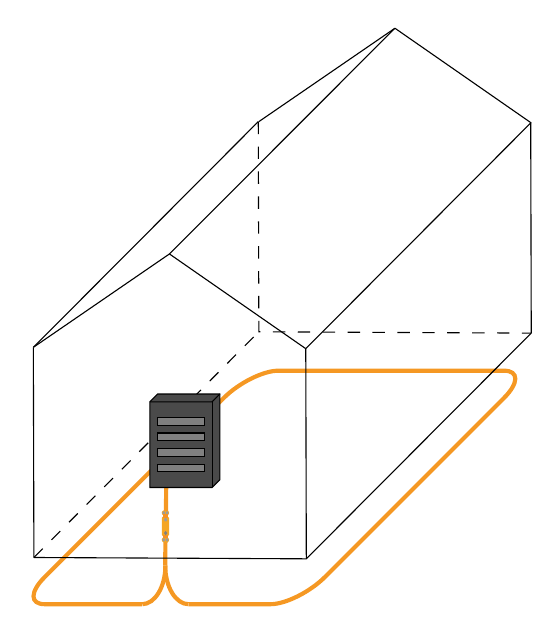
\begin{tikzpicture}[x=0.75pt,y=0.75pt,yscale=-0.75,xscale=0.75]
%uncomment if require: \path (0,481); %set diagram left start at 0, and has height of 481

%Straight Lines [id:da30799843530611115] 
\draw [color={rgb, 255:red, 245; green, 152; blue, 35 }  ,draw opacity=1 ][line width=1.5]    (240,360) -- (239.84,375.16) ;
%Straight Lines [id:da5305354409070833] 
\draw  [dash pattern={on 4.5pt off 4.5pt}]  (299.65,90) -- (300,225) -- (475,225.85) ;
%Straight Lines [id:da20935901156494685] 
\draw  [dash pattern={on 4.5pt off 4.5pt}]  (155.5,370) -- (300,225) ;
%Straight Lines [id:da9663799350386381] 
\draw    (155.15,235) -- (155.5,370) ;
%Straight Lines [id:da6956273497313757] 
\draw    (474.65,90.85) -- (475,225.85) ;
%Straight Lines [id:da46520744988670826] 
\draw    (155.15,235) -- (299.65,90) ;
%Straight Lines [id:da18568330552579893] 
\draw    (242.57,175) -- (330.15,235.85) ;
%Straight Lines [id:da08951823691400396] 
\draw    (155.15,235) -- (242.57,175) ;
%Straight Lines [id:da3765980997616395] 
\draw    (387.43,30) -- (475,90.85) ;
%Straight Lines [id:da20425329876761578] 
\draw    (300,90) -- (387.43,30) ;
%Straight Lines [id:da3978892908876972] 
\draw    (387.43,30) -- (242.57,175) ;
%Straight Lines [id:da3001438899283537] 
\draw    (474.65,90.85) -- (330.15,235.85) ;
%Rounded Rect [id:dp877203358644785] 
\draw  [color={rgb, 255:red, 245; green, 152; blue, 35 }  ,draw opacity=1 ][line width=1.5]  (277.5,267.5) .. controls (287.16,257.84) and (302.84,250) .. (312.5,250) -- (457.5,250) .. controls (467.16,250) and (467.16,257.84) .. (457.5,267.5) -- (342.5,382.5) .. controls (332.84,392.16) and (317.16,400) .. (307.5,400) -- (162.5,400) .. controls (152.84,400) and (152.84,392.16) .. (162.5,382.5) -- cycle ;
%Straight Lines [id:da4856516771678496] 
\draw    (330.15,235.85) -- (330.5,370.85) ;
%Straight Lines [id:da20084021876297198] 
\draw    (155.5,370) -- (330.5,370.85) -- (475,225.85) ;
%Straight Lines [id:da14498872282205144] 
\draw [color={rgb, 255:red, 255; green, 255; blue, 255 }  ,draw opacity=1 ][line width=3]    (225.15,400) -- (254.97,400) ;
%Shape: Arc [id:dp8164801831387742] 
\draw  [draw opacity=0][line width=1.5]  (254.97,400) .. controls (254.93,400) and (254.89,400) .. (254.84,400) .. controls (246.59,400) and (239.9,388.89) .. (239.84,375.16) -- (254.84,375) -- cycle ; \draw  [color={rgb, 255:red, 245; green, 152; blue, 35 }  ,draw opacity=1 ][line width=1.5]  (254.97,400) .. controls (254.93,400) and (254.89,400) .. (254.84,400) .. controls (246.59,400) and (239.9,388.89) .. (239.84,375.16) ;
%Shape: Arc [id:dp4891672557856719] 
\draw  [draw opacity=0][line width=1.5]  (240,375.38) .. controls (239.88,388.93) and (233.29,399.86) .. (225.15,400) -- (225,375) -- cycle ; \draw  [color={rgb, 255:red, 245; green, 152; blue, 35 }  ,draw opacity=1 ][line width=1.5]  (240,375.38) .. controls (239.88,388.93) and (233.29,399.86) .. (225.15,400) ;
%Rounded Rect [id:dp13850405546686684] 
\draw  [color={rgb, 255:red, 245; green, 166; blue, 35 }  ,draw opacity=1 ][fill={rgb, 255:red, 245; green, 166; blue, 35 }  ,fill opacity=1 ] (238,341.33) .. controls (238,340.6) and (238.6,340) .. (239.33,340) -- (240.67,340) .. controls (241.4,340) and (242,340.6) .. (242,341.33) -- (242,341.33) .. controls (242,342.07) and (241.4,342.67) .. (240.67,342.67) -- (239.33,342.67) .. controls (238.6,342.67) and (238,342.07) .. (238,341.33) -- cycle ;
%Shape: Polygon [id:dp012352628803113719] 
\draw  [color={rgb, 255:red, 155; green, 155; blue, 155 }  ,draw opacity=1 ][fill={rgb, 255:red, 155; green, 155; blue, 155 }  ,fill opacity=1 ] (241.6,341.33) -- (241.35,341.91) -- (240.85,341.91) -- (240.6,341.33) -- (240.85,340.76) -- (241.35,340.76) -- cycle ;
%Shape: Polygon [id:dp617840417972505] 
\draw  [color={rgb, 255:red, 155; green, 155; blue, 155 }  ,draw opacity=1 ][fill={rgb, 255:red, 155; green, 155; blue, 155 }  ,fill opacity=1 ] (239.4,341.33) -- (239.15,341.91) -- (238.65,341.91) -- (238.4,341.33) -- (238.65,340.76) -- (239.15,340.76) -- cycle ;

%Rounded Rect [id:dp29263936410769587] 
\draw  [color={rgb, 255:red, 245; green, 166; blue, 35 }  ,draw opacity=1 ][fill={rgb, 255:red, 245; green, 166; blue, 35 }  ,fill opacity=1 ] (238,358.67) .. controls (238,357.93) and (238.6,357.33) .. (239.33,357.33) -- (240.67,357.33) .. controls (241.4,357.33) and (242,357.93) .. (242,358.67) -- (242,358.67) .. controls (242,359.4) and (241.4,360) .. (240.67,360) -- (239.33,360) .. controls (238.6,360) and (238,359.4) .. (238,358.67) -- cycle ;
%Shape: Polygon [id:dp39786342275295183] 
\draw  [color={rgb, 255:red, 155; green, 155; blue, 155 }  ,draw opacity=1 ][fill={rgb, 255:red, 155; green, 155; blue, 155 }  ,fill opacity=1 ] (241.6,358.67) -- (241.35,359.24) -- (240.85,359.24) -- (240.6,358.67) -- (240.85,358.09) -- (241.35,358.09) -- cycle ;
%Shape: Polygon [id:dp030526214760367876] 
\draw  [color={rgb, 255:red, 155; green, 155; blue, 155 }  ,draw opacity=1 ][fill={rgb, 255:red, 155; green, 155; blue, 155 }  ,fill opacity=1 ] (239.4,358.67) -- (239.15,359.24) -- (238.65,359.24) -- (238.4,358.67) -- (238.65,358.09) -- (239.15,358.09) -- cycle ;

%Rounded Rect [id:dp9275012189629497] 
\draw  [color={rgb, 255:red, 245; green, 166; blue, 35 }  ,draw opacity=1 ][fill={rgb, 255:red, 245; green, 166; blue, 35 }  ,fill opacity=1 ] (238,344.73) .. controls (238,344.33) and (238.33,344) .. (238.73,344) -- (241.27,344) .. controls (241.67,344) and (242,344.33) .. (242,344.73) -- (242,355.27) .. controls (242,355.67) and (241.67,356) .. (241.27,356) -- (238.73,356) .. controls (238.33,356) and (238,355.67) .. (238,355.27) -- cycle ;
%Shape: Polygon [id:dp7623761074716651] 
\draw  [color={rgb, 255:red, 155; green, 155; blue, 155 }  ,draw opacity=1 ][fill={rgb, 255:red, 155; green, 155; blue, 155 }  ,fill opacity=1 ] (240.69,345.73) -- (240.4,346.39) -- (239.83,346.39) -- (239.54,345.73) -- (239.83,345.07) -- (240.4,345.07) -- cycle ;
%Shape: Rectangle [id:dp25144871820084] 
\draw  [color={rgb, 255:red, 245; green, 145; blue, 35 }  ,draw opacity=1 ][fill={rgb, 255:red, 245; green, 145; blue, 35 }  ,fill opacity=1 ] (241,356) -- (239,356) -- (239,357.33) -- (241,357.33) -- cycle ;
%Shape: Rectangle [id:dp07880374452402983] 
\draw  [color={rgb, 255:red, 245; green, 145; blue, 35 }  ,draw opacity=1 ][fill={rgb, 255:red, 245; green, 145; blue, 35 }  ,fill opacity=1 ] (241,342.67) -- (239,342.67) -- (239,344) -- (241,344) -- cycle ;
%Shape: Ellipse [id:dp8682429169918172] 
\draw  [color={rgb, 255:red, 128; green, 128; blue, 128 }  ,draw opacity=1 ][fill={rgb, 255:red, 128; green, 128; blue, 128 }  ,fill opacity=1 ] (240.8,354.33) .. controls (240.8,353.85) and (240.51,353.47) .. (240.15,353.47) .. controls (239.79,353.47) and (239.5,353.85) .. (239.5,354.33) .. controls (239.5,354.81) and (239.79,355.2) .. (240.15,355.2) .. controls (240.51,355.2) and (240.8,354.81) .. (240.8,354.33) -- cycle ;

%Straight Lines [id:da5244519047151425] 
\draw [color={rgb, 255:red, 245; green, 152; blue, 35 }  ,draw opacity=1 ][line width=1.5]    (240.49,324.84) -- (240.33,340) ;
%Shape: Cube [id:dp960688551107607] 
\draw  [fill={rgb, 255:red, 74; green, 74; blue, 74 }  ,fill opacity=1 ] (230,270) -- (235,265) -- (275,265) -- (275,320) -- (270,325) -- (230,325) -- cycle ; \draw   (275,265) -- (270,270) -- (230,270) ; \draw   (270,270) -- (270,325) ;
%Shape: Rectangle [id:dp6308555982138916] 
\draw  [fill={rgb, 255:red, 128; green, 128; blue, 128 }  ,fill opacity=1 ] (235,310) -- (265,310) -- (265,315) -- (235,315) -- cycle ;
%Shape: Rectangle [id:dp6763259519643228] 
\draw  [fill={rgb, 255:red, 128; green, 128; blue, 128 }  ,fill opacity=1 ] (235,300) -- (265,300) -- (265,305) -- (235,305) -- cycle ;
%Shape: Rectangle [id:dp688777309088791] 
\draw  [fill={rgb, 255:red, 128; green, 128; blue, 128 }  ,fill opacity=1 ] (235,290) -- (265,290) -- (265,295) -- (235,295) -- cycle ;
%Shape: Rectangle [id:dp5453582139616918] 
\draw  [fill={rgb, 255:red, 128; green, 128; blue, 128 }  ,fill opacity=1 ] (235,280) -- (265,280) -- (265,285) -- (235,285) -- cycle ;




\end{tikzpicture}

\end{figure}

%\end{document}



\paragraph{Câble en tranchée}
Si la mise en \oe{}uvre de la boucle à fond de fouille n'est pas possible (bâtiment existant par exemple), on peut réaliser la mise à la terre de l'installation électrique par l'installation d'un câble en tranchée en respectant les règles de pose explicité dans le schéma \superref{fig:cable_tranchee}.\\
Le conducteur utilisé doit aussi présenter une section minimale selon le matériau choisi :
\begin{itemize}
\item câble de cuivre nu de \SI{25}{\square\milli\meter}\,;
\item câble en acier de \SI{95}{\square\milli\meter}.
\end{itemize}

%--------------------------------------
%ELECTROTECHNIQUE - SCHEMA DE LIAISON A LA TERRE
%--------------------------------------

%utiliser les environnement \begin{comment} \end{comment} pour mettre en commentaire le préambule une fois la programmation appelée dans le document maître (!ne pas oublier de mettre en commentaire \end{document}!)

\begin{comment}

\documentclass[a4paper, 11pt, twoside, fleqn]{memoir}

\usepackage{AOCDTF}

\marqueurchapitre

%lien d'édition des figures Tikz sur le site mathcha.io (rajouter le lien d'une modification effectuée sur la figure tikz avec le nom du modificateur car il n'y a qu'un lien par compte)

%lien mathcha Bruno Douchy : https://www.mathcha.io/editor/KxQm6cWBUm3T7kkkkVH5ynXwpHOKYnVpc0pjJvM

%--------------------------------------
%corps du document
%--------------------------------------

\begin{document} %corps du document
	\openleft %début de chapitre à gauche

\end{comment}
\begin{figure}[H]
\caption{Câble en tranchée\label{fig:cable_tranchee}}
\tikzset{every picture/.style={line width=0.75pt}} %set default line width to 0.75pt        

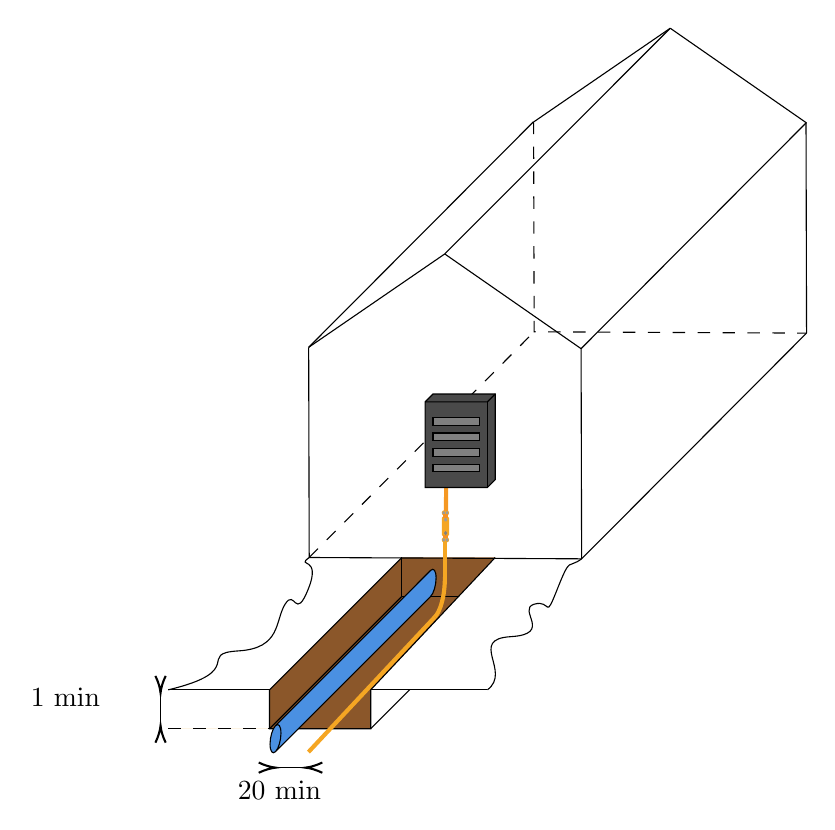
\begin{tikzpicture}[x=0.75pt,y=0.75pt,yscale=-0.75,xscale=0.75]
%uncomment if require: \path (0,751); %set diagram left start at 0, and has height of 751

%Straight Lines [id:da7829987710081011] 
\draw [fill={rgb, 255:red, 139; green, 87; blue, 42 }  ,fill opacity=1 ]   (280,340) -- (200,425) -- (200,450) -- (135,450) -- (135,425) -- (135,425) -- (220,340) ;
%Straight Lines [id:da49257416521092223] 
\draw    (220,365) -- (257,365) ;
%Straight Lines [id:da9081598274402687] 
\draw  [dash pattern={on 4.5pt off 4.5pt}]  (304.65,60) -- (305,195) -- (480,195.85) ;
%Straight Lines [id:da6348721638486958] 
\draw  [dash pattern={on 4.5pt off 4.5pt}]  (160.5,340) -- (305,195) ;
%Straight Lines [id:da1909522090160657] 
\draw    (160.15,205) -- (160.5,340) ;
%Straight Lines [id:da7207753640653374] 
\draw    (479.65,60.85) -- (480,195.85) ;
%Straight Lines [id:da6535753192189023] 
\draw    (160.15,205) -- (304.65,60) ;
%Straight Lines [id:da79950742566739] 
\draw    (247.57,145) -- (335.15,205.85) ;
%Straight Lines [id:da5547090580418039] 
\draw    (160.15,205) -- (247.57,145) ;
%Straight Lines [id:da920533856446613] 
\draw    (392.43,0) -- (480,60.85) ;
%Straight Lines [id:da11208478674638356] 
\draw    (305,60) -- (392.43,0) ;
%Straight Lines [id:da39788580291104303] 
\draw    (392.43,0) -- (247.57,145) ;
%Straight Lines [id:da7411479557367767] 
\draw    (479.65,60.85) -- (335.15,205.85) ;
%Straight Lines [id:da21547405248779972] 
\draw    (335.15,205.85) -- (335.5,340.85) ;
%Rounded Rect [id:dp28722339808467556] 
\draw  [color={rgb, 255:red, 245; green, 166; blue, 35 }  ,draw opacity=1 ][fill={rgb, 255:red, 245; green, 166; blue, 35 }  ,fill opacity=1 ] (246,311.33) .. controls (246,310.6) and (246.6,310) .. (247.33,310) -- (248.67,310) .. controls (249.4,310) and (250,310.6) .. (250,311.33) -- (250,311.33) .. controls (250,312.07) and (249.4,312.67) .. (248.67,312.67) -- (247.33,312.67) .. controls (246.6,312.67) and (246,312.07) .. (246,311.33) -- cycle ;
%Shape: Polygon [id:dp4090325935091489] 
\draw  [color={rgb, 255:red, 155; green, 155; blue, 155 }  ,draw opacity=1 ][fill={rgb, 255:red, 155; green, 155; blue, 155 }  ,fill opacity=1 ] (249.6,311.33) -- (249.35,311.91) -- (248.85,311.91) -- (248.6,311.33) -- (248.85,310.76) -- (249.35,310.76) -- cycle ;
%Shape: Polygon [id:dp35689183508447087] 
\draw  [color={rgb, 255:red, 155; green, 155; blue, 155 }  ,draw opacity=1 ][fill={rgb, 255:red, 155; green, 155; blue, 155 }  ,fill opacity=1 ] (247.4,311.33) -- (247.15,311.91) -- (246.65,311.91) -- (246.4,311.33) -- (246.65,310.76) -- (247.15,310.76) -- cycle ;

%Rounded Rect [id:dp06111128559002643] 
\draw  [color={rgb, 255:red, 245; green, 166; blue, 35 }  ,draw opacity=1 ][fill={rgb, 255:red, 245; green, 166; blue, 35 }  ,fill opacity=1 ] (246,328.67) .. controls (246,327.93) and (246.6,327.33) .. (247.33,327.33) -- (248.67,327.33) .. controls (249.4,327.33) and (250,327.93) .. (250,328.67) -- (250,328.67) .. controls (250,329.4) and (249.4,330) .. (248.67,330) -- (247.33,330) .. controls (246.6,330) and (246,329.4) .. (246,328.67) -- cycle ;
%Shape: Polygon [id:dp7859094987135327] 
\draw  [color={rgb, 255:red, 155; green, 155; blue, 155 }  ,draw opacity=1 ][fill={rgb, 255:red, 155; green, 155; blue, 155 }  ,fill opacity=1 ] (249.6,328.67) -- (249.35,329.24) -- (248.85,329.24) -- (248.6,328.67) -- (248.85,328.09) -- (249.35,328.09) -- cycle ;
%Shape: Polygon [id:dp0947001255145501] 
\draw  [color={rgb, 255:red, 155; green, 155; blue, 155 }  ,draw opacity=1 ][fill={rgb, 255:red, 155; green, 155; blue, 155 }  ,fill opacity=1 ] (247.4,328.67) -- (247.15,329.24) -- (246.65,329.24) -- (246.4,328.67) -- (246.65,328.09) -- (247.15,328.09) -- cycle ;

%Rounded Rect [id:dp5387904806018837] 
\draw  [color={rgb, 255:red, 245; green, 166; blue, 35 }  ,draw opacity=1 ][fill={rgb, 255:red, 245; green, 166; blue, 35 }  ,fill opacity=1 ] (246,314.73) .. controls (246,314.33) and (246.33,314) .. (246.73,314) -- (249.27,314) .. controls (249.67,314) and (250,314.33) .. (250,314.73) -- (250,325.27) .. controls (250,325.67) and (249.67,326) .. (249.27,326) -- (246.73,326) .. controls (246.33,326) and (246,325.67) .. (246,325.27) -- cycle ;
%Shape: Polygon [id:dp6617291355484505] 
\draw  [color={rgb, 255:red, 155; green, 155; blue, 155 }  ,draw opacity=1 ][fill={rgb, 255:red, 155; green, 155; blue, 155 }  ,fill opacity=1 ] (248.69,315.73) -- (248.4,316.39) -- (247.83,316.39) -- (247.54,315.73) -- (247.83,315.07) -- (248.4,315.07) -- cycle ;
%Shape: Rectangle [id:dp3731803592403742] 
\draw  [color={rgb, 255:red, 245; green, 145; blue, 35 }  ,draw opacity=1 ][fill={rgb, 255:red, 245; green, 145; blue, 35 }  ,fill opacity=1 ] (249,326) -- (247,326) -- (247,327.33) -- (249,327.33) -- cycle ;
%Shape: Rectangle [id:dp13543640418430414] 
\draw  [color={rgb, 255:red, 245; green, 145; blue, 35 }  ,draw opacity=1 ][fill={rgb, 255:red, 245; green, 145; blue, 35 }  ,fill opacity=1 ] (249,312.67) -- (247,312.67) -- (247,314) -- (249,314) -- cycle ;
%Shape: Ellipse [id:dp009996283185936261] 
\draw  [color={rgb, 255:red, 128; green, 128; blue, 128 }  ,draw opacity=1 ][fill={rgb, 255:red, 128; green, 128; blue, 128 }  ,fill opacity=1 ] (248.8,324.33) .. controls (248.8,323.85) and (248.51,323.47) .. (248.15,323.47) .. controls (247.79,323.47) and (247.5,323.85) .. (247.5,324.33) .. controls (247.5,324.81) and (247.79,325.2) .. (248.15,325.2) .. controls (248.51,325.2) and (248.8,324.81) .. (248.8,324.33) -- cycle ;

%Straight Lines [id:da07044954250685276] 
\draw [color={rgb, 255:red, 245; green, 152; blue, 35 }  ,draw opacity=1 ][line width=1.5]    (248.49,294.84) -- (248.33,310) ;
%Shape: Cube [id:dp8957361009096318] 
\draw  [fill={rgb, 255:red, 74; green, 74; blue, 74 }  ,fill opacity=1 ] (235,240) -- (240,235) -- (280,235) -- (280,290) -- (275,295) -- (235,295) -- cycle ; \draw   (280,235) -- (275,240) -- (235,240) ; \draw   (275,240) -- (275,295) ;
%Shape: Rectangle [id:dp22048605405624178] 
\draw  [fill={rgb, 255:red, 128; green, 128; blue, 128 }  ,fill opacity=1 ] (240,280) -- (270,280) -- (270,285) -- (240,285) -- cycle ;
%Shape: Rectangle [id:dp38722589110484673] 
\draw  [fill={rgb, 255:red, 128; green, 128; blue, 128 }  ,fill opacity=1 ] (240,270) -- (270,270) -- (270,275) -- (240,275) -- cycle ;
%Shape: Rectangle [id:dp6742075818101974] 
\draw  [fill={rgb, 255:red, 128; green, 128; blue, 128 }  ,fill opacity=1 ] (240,260) -- (270,260) -- (270,265) -- (240,265) -- cycle ;
%Shape: Rectangle [id:dp8945073743205151] 
\draw  [fill={rgb, 255:red, 128; green, 128; blue, 128 }  ,fill opacity=1 ] (240,250) -- (270,250) -- (270,255) -- (240,255) -- cycle ;
%Shape: Arc [id:dp4869608729068412] 
\draw  [draw opacity=0][line width=1.5]  (247.67,352.54) .. controls (247.66,364.36) and (244.94,374.42) .. (241.14,378.3) -- (237.67,352.5) -- cycle ; \draw  [color={rgb, 255:red, 245; green, 166; blue, 35 }  ,draw opacity=1 ][line width=1.5]  (247.67,352.54) .. controls (247.66,364.36) and (244.94,374.42) .. (241.14,378.3) ;
%Straight Lines [id:da9150475387692276] 
\draw [color={rgb, 255:red, 245; green, 166; blue, 35 }  ,draw opacity=1 ][line width=1.5]    (160,465) -- (241.14,378.3) ;
%Straight Lines [id:da2033450004552232] 
\draw [fill={rgb, 255:red, 245; green, 166; blue, 35 }  ,fill opacity=1 ]   (70,425) -- (135,425) ;
%Straight Lines [id:da7151214616154821] 
\draw    (200,425) -- (275,425) ;
%Curve Lines [id:da6063582718063134] 
\draw    (70,425) .. controls (121.5,412.67) and (87.4,401.64) .. (115,400) .. controls (142.6,398.36) and (138.42,380.61) .. (145,370) .. controls (151.58,359.39) and (151.4,381.64) .. (160,360) .. controls (168.6,338.36) and (151.6,346.68) .. (160.5,340) ;
%Curve Lines [id:da7510759130219333] 
\draw    (275,425) .. controls (290.74,413.2) and (262.4,392.49) .. (290,390.85) .. controls (317.6,389.22) and (293.6,373.36) .. (305,370) .. controls (316.4,366.64) and (311.4,381.64) .. (320,360) .. controls (328.6,338.36) and (326.6,347.53) .. (335.5,340.85) ;
%Straight Lines [id:da3682420377901341] 
\draw    (480,195.85) -- (335.5,340.85) ;
%Straight Lines [id:da9913786842235923] 
\draw    (220,365) -- (135,450) ;
%Straight Lines [id:da8269394900324805] 
\draw    (200,450) -- (225,425) ;
%Straight Lines [id:da9808722000068587] 
\draw    (220,340) -- (220,365) ;
%Straight Lines [id:da3541321557731596] 
\draw    (160.5,340) -- (335.5,340.85) ;
%Straight Lines [id:da5783336689263071] 
\draw    (65,427) -- (65,448) ;
\draw [shift={(65,448)}, rotate = 90] [color={rgb, 255:red, 0; green, 0; blue, 0 }  ][line width=0.75]    (10.93,-3.29) .. controls (6.95,-1.4) and (3.31,-0.3) .. (0,0) .. controls (3.31,0.3) and (6.95,1.4) .. (10.93,3.29)   ;
\draw [shift={(65,427)}, rotate = 270] [color={rgb, 255:red, 0; green, 0; blue, 0 }  ][line width=0.75]    (10.93,-3.29) .. controls (6.95,-1.4) and (3.31,-0.3) .. (0,0) .. controls (3.31,0.3) and (6.95,1.4) .. (10.93,3.29)   ;
%Straight Lines [id:da7565418229148708] 
\draw [color={rgb, 255:red, 245; green, 166; blue, 35 }  ,draw opacity=1 ][line width=1.5]    (247.67,330) -- (247.67,352.54) ;
%Shape: Can [id:dp7267813341154139] 
\draw  [fill={rgb, 255:red, 74; green, 144; blue, 226 }  ,fill opacity=1 ] (138.85,448.03) -- (238.5,348.28) .. controls (240.44,346.34) and (242.01,348.51) .. (242.01,353.13) .. controls (242.01,357.74) and (240.44,363.06) .. (238.5,365) -- (138.85,464.75) .. controls (136.91,466.69) and (135.34,464.52) .. (135.34,459.9) .. controls (135.34,455.29) and (136.91,449.97) .. (138.85,448.03) .. controls (140.79,446.09) and (142.36,448.26) .. (142.36,452.88) .. controls (142.36,457.5) and (140.79,462.81) .. (138.85,464.75) ;
%Straight Lines [id:da42695123304320515] 
\draw    (158,475) -- (139,475) ;
\draw [shift={(139,475)}, rotate = 180] [color={rgb, 255:red, 0; green, 0; blue, 0 }  ][line width=0.75]    (10.93,-3.29) .. controls (6.95,-1.4) and (3.31,-0.3) .. (0,0) .. controls (3.31,0.3) and (6.95,1.4) .. (10.93,3.29)   ;
\draw [shift={(158,475)}, rotate = 360] [color={rgb, 255:red, 0; green, 0; blue, 0 }  ][line width=0.75]    (10.93,-3.29) .. controls (6.95,-1.4) and (3.31,-0.3) .. (0,0) .. controls (3.31,0.3) and (6.95,1.4) .. (10.93,3.29)   ;
%Straight Lines [id:da04967441192853961] 
\draw [fill={rgb, 255:red, 245; green, 166; blue, 35 }  ,fill opacity=1 ] [dash pattern={on 4.5pt off 4.5pt}]  (70,450) -- (135,450) ;

% Text Node
\draw (-20,422) node [anchor=north west][inner sep=0.75pt]   [align=left] {\SI{1}{\meter} min};
% Text Node
\draw (113,482) node [anchor=north west][inner sep=0.75pt]   [align=left] {\SI{20}{\centi\meter} min};


\end{tikzpicture}

\end{figure}

%\end{document}



\paragraph{Piquet de terre}
Si aucune des deux solutions précédentes n'est envisageable, on peut réaliser la prise de terre au moyen d'un piquet enfoncé dans le sol en respectant les règles de pose explicité dans le schéma \superref{fig:piquet_terre}.\\
Le piquet utilisé doit aussi présenter une section ou une surface minimale selon le matériau choisi :
\begin{itemize}
\item tube en acier de \SI{25}{\milli\meter} de diamètre\,;
\item profilé en acier de \SI{60}{\square\milli\meter} de diamètre\,;
\item une barre de cuivre ou d'acier cuivré de \SI{15}{\square\milli\meter} de diamètre.
\end{itemize}

%--------------------------------------
%ELECTROTECHNIQUE - SCHEMA DE LIAISON A LA TERRE
%--------------------------------------

%utiliser les environnement \begin{comment} \end{comment} pour mettre en commentaire le préambule une fois la programmation appelée dans le document maître (!ne pas oublier de mettre en commentaire \end{document}!)

\begin{comment}

\documentclass[a4paper, 11pt, twoside, fleqn]{memoir}

\usepackage{AOCDTF}

\marqueurchapitre

%lien d'édition des figures Tikz sur le site mathcha.io (rajouter le lien d'une modification effectuée sur la figure tikz avec le nom du modificateur car il n'y a qu'un lien par compte)

%lien mathcha Bruno Douchy : https://www.mathcha.io/editor/nlpozt7QSeWtkXQqWyi5zjE93SXrZeriPKxP5

%--------------------------------------
%corps du document
%--------------------------------------

\begin{document} %corps du document
	\openleft %début de chapitre à gauche

\end{comment}

\begin{figure}[H]
\caption{Piquet de terre\label{fig:piquet_terre}}


\tikzset{every picture/.style={line width=0.75pt}} %set default line width to 0.75pt        

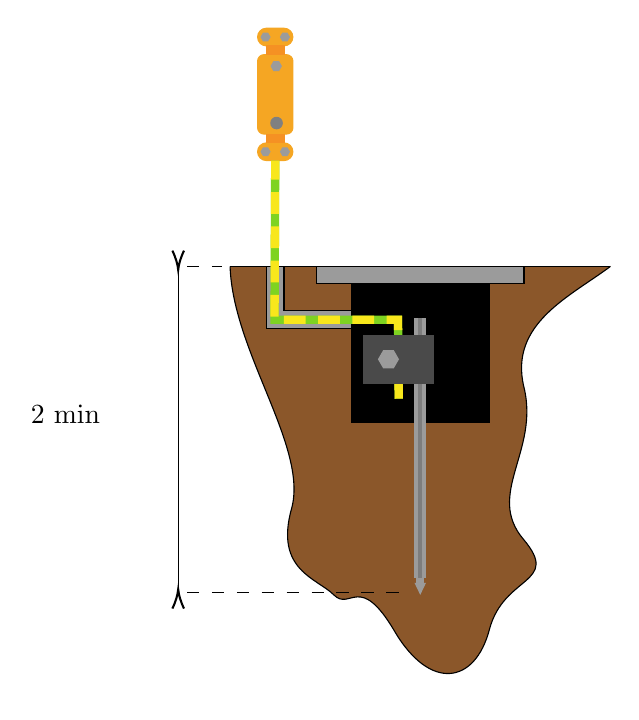
\begin{tikzpicture}[x=0.75pt,y=0.75pt,yscale=-0.85,xscale=0.85]
%uncomment if require: \path (0,484); %set diagram left start at 0, and has height of 484

%Rounded Rect [id:dp6359600964219599] 
\draw  [color={rgb, 255:red, 245; green, 166; blue, 35 }  ,draw opacity=1 ][fill={rgb, 255:red, 245; green, 166; blue, 35 }  ,fill opacity=1 ] (430,80) .. controls (430,77.24) and (432.24,75) .. (435,75) -- (445,75) .. controls (447.76,75) and (450,77.24) .. (450,80) -- (450,80) .. controls (450,82.76) and (447.76,85) .. (445,85) -- (435,85) .. controls (432.24,85) and (430,82.76) .. (430,80) -- cycle ;
%Shape: Regular Polygon [id:dp5335311391934556] 
\draw  [color={rgb, 255:red, 155; green, 155; blue, 155 }  ,draw opacity=1 ][fill={rgb, 255:red, 155; green, 155; blue, 155 }  ,fill opacity=1 ] (448,80) -- (446.75,82.17) -- (444.25,82.17) -- (443,80) -- (444.25,77.83) -- (446.75,77.83) -- cycle ;
%Shape: Regular Polygon [id:dp7077127128502503] 
\draw  [color={rgb, 255:red, 155; green, 155; blue, 155 }  ,draw opacity=1 ][fill={rgb, 255:red, 155; green, 155; blue, 155 }  ,fill opacity=1 ] (437,80) -- (435.75,82.17) -- (433.25,82.17) -- (432,80) -- (433.25,77.83) -- (435.75,77.83) -- cycle ;

%Rounded Rect [id:dp26376134008390595] 
\draw  [color={rgb, 255:red, 245; green, 166; blue, 35 }  ,draw opacity=1 ][fill={rgb, 255:red, 245; green, 166; blue, 35 }  ,fill opacity=1 ] (430,145) .. controls (430,142.24) and (432.24,140) .. (435,140) -- (445,140) .. controls (447.76,140) and (450,142.24) .. (450,145) -- (450,145) .. controls (450,147.76) and (447.76,150) .. (445,150) -- (435,150) .. controls (432.24,150) and (430,147.76) .. (430,145) -- cycle ;
%Shape: Regular Polygon [id:dp6433620371225686] 
\draw  [color={rgb, 255:red, 155; green, 155; blue, 155 }  ,draw opacity=1 ][fill={rgb, 255:red, 155; green, 155; blue, 155 }  ,fill opacity=1 ] (448,145) -- (446.75,147.17) -- (444.25,147.17) -- (443,145) -- (444.25,142.83) -- (446.75,142.83) -- cycle ;
%Shape: Regular Polygon [id:dp6874144748844591] 
\draw  [color={rgb, 255:red, 155; green, 155; blue, 155 }  ,draw opacity=1 ][fill={rgb, 255:red, 155; green, 155; blue, 155 }  ,fill opacity=1 ] (437,145) -- (435.75,147.17) -- (433.25,147.17) -- (432,145) -- (433.25,142.83) -- (435.75,142.83) -- cycle ;

%Rounded Rect [id:dp6592130378481749] 
\draw  [color={rgb, 255:red, 245; green, 166; blue, 35 }  ,draw opacity=1 ][fill={rgb, 255:red, 245; green, 166; blue, 35 }  ,fill opacity=1 ] (430,93.67) .. controls (430,91.64) and (431.64,90) .. (433.67,90) -- (446.33,90) .. controls (448.36,90) and (450,91.64) .. (450,93.67) -- (450,131.33) .. controls (450,133.36) and (448.36,135) .. (446.33,135) -- (433.67,135) .. controls (431.64,135) and (430,133.36) .. (430,131.33) -- cycle ;
%Shape: Regular Polygon [id:dp28570519258745464] 
\draw  [color={rgb, 255:red, 155; green, 155; blue, 155 }  ,draw opacity=1 ][fill={rgb, 255:red, 155; green, 155; blue, 155 }  ,fill opacity=1 ] (443.43,96.48) -- (442,98.96) -- (439.14,98.96) -- (437.7,96.48) -- (439.14,94) -- (442,94) -- cycle ;
%Shape: Rectangle [id:dp1437469136470797] 
\draw  [color={rgb, 255:red, 245; green, 145; blue, 35 }  ,draw opacity=1 ][fill={rgb, 255:red, 245; green, 145; blue, 35 }  ,fill opacity=1 ] (445,135) -- (435,135) -- (435,140) -- (445,140) -- cycle ;
%Shape: Rectangle [id:dp5260720882019565] 
\draw  [color={rgb, 255:red, 245; green, 145; blue, 35 }  ,draw opacity=1 ][fill={rgb, 255:red, 245; green, 145; blue, 35 }  ,fill opacity=1 ] (445,85) -- (435,85) -- (435,90) -- (445,90) -- cycle ;
%Shape: Circle [id:dp38824432139246823] 
\draw  [color={rgb, 255:red, 128; green, 128; blue, 128 }  ,draw opacity=1 ][fill={rgb, 255:red, 128; green, 128; blue, 128 }  ,fill opacity=1 ] (444,128.75) .. controls (444,126.96) and (442.54,125.5) .. (440.75,125.5) .. controls (438.96,125.5) and (437.5,126.96) .. (437.5,128.75) .. controls (437.5,130.54) and (438.96,132) .. (440.75,132) .. controls (442.54,132) and (444,130.54) .. (444,128.75) -- cycle ;

%Curve Lines [id:da1902694494170415] 
\draw [fill={rgb, 255:red, 139; green, 87; blue, 42 }  ,fill opacity=1 ]   (414.41,210) .. controls (416.02,258.76) and (458.92,312.57) .. (449.23,347.41) .. controls (439.53,382.24) and (463.78,386.73) .. (473.21,396.19) .. controls (482.63,405.66) and (487.64,382.87) .. (507.69,416.85) .. controls (527.73,450.84) and (553.21,446.92) .. (561.4,415.79) .. controls (569.6,384.67) and (602.15,390.07) .. (580.62,364.59) .. controls (559.09,339.12) and (589.8,314.72) .. (581,278.6) .. controls (572.2,242.47) and (607.23,227.08) .. (630,210) ;
%Shape: Rectangle [id:dp6184966297023284] 
\draw  [color={rgb, 255:red, 0; green, 0; blue, 0 }  ,draw opacity=1 ][fill={rgb, 255:red, 155; green, 155; blue, 155 }  ,fill opacity=1 ] (463.41,210) -- (581,210) -- (581,219.8) -- (463.41,219.8) -- cycle ;
%Straight Lines [id:da003175631258122258] 
\draw [fill={rgb, 255:red, 139; green, 87; blue, 42 }  ,fill opacity=1 ]   (414.41,210) -- (630,210) ;
%Shape: Rectangle [id:dp15550713014547501] 
\draw  [fill={rgb, 255:red, 0; green, 0; blue, 0 }  ,fill opacity=1 ] (483.01,219.8) -- (561.4,219.8) -- (561.4,298.2) -- (483.01,298.2) -- cycle ;
%Straight Lines [id:da6327089569131619] 
\draw [color={rgb, 255:red, 155; green, 155; blue, 155 }  ,draw opacity=1 ][line width=3]    (522.2,239.4) -- (522.2,390.19) ;
\draw [shift={(522.2,396.19)}, rotate = 270] [fill={rgb, 255:red, 155; green, 155; blue, 155 }  ,fill opacity=1 ][line width=0.08]  [draw opacity=0] (6.79,-3.26) -- (0,0) -- (6.79,3.26) -- cycle    ;
%Straight Lines [id:da7643156131849724] 
\draw [color={rgb, 255:red, 155; green, 155; blue, 155 }  ,draw opacity=1 ][line width=4.5]    (522.2,239.4) -- (522.2,386.39) ;
%Straight Lines [id:da9437529376818724] 
\draw [color={rgb, 255:red, 74; green, 74; blue, 74 }  ,draw opacity=0.37 ][line width=1.5]    (522.2,239.4) -- (522.2,386.39) ;
%Straight Lines [id:da45205830376086187] 
\draw [color={rgb, 255:red, 0; green, 0; blue, 0 }  ,draw opacity=1 ][fill={rgb, 255:red, 155; green, 155; blue, 155 }  ,fill opacity=1 ]   (435,210) -- (445,210) -- (445,235) -- (483,235) -- (483,245) -- (435,245) -- cycle ;
%Straight Lines [id:da9689359180145172] 
\draw [color={rgb, 255:red, 126; green, 211; blue, 33 }  ,draw opacity=1 ][line width=3]    (440,150) -- (439.6,240.26) -- (509.6,240.26) -- (510,285) ;
%Straight Lines [id:da44161159619032986] 
\draw [color={rgb, 255:red, 248; green, 231; blue, 28 }  ,draw opacity=1 ][line width=3]  [dash pattern={on 7.88pt off 4.5pt}]  (510,285) -- (509.6,240.26) -- (439.6,240.26) -- (440,150) ;
%Shape: Rectangle [id:dp5856416399734485] 
\draw  [color={rgb, 255:red, 74; green, 74; blue, 74 }  ,draw opacity=1 ][fill={rgb, 255:red, 74; green, 74; blue, 74 }  ,fill opacity=1 ] (490.2,249.16) -- (529.4,249.16) -- (529.4,276.11) -- (490.2,276.11) -- cycle ;
%Shape: Regular Polygon [id:dp7503784010969258] 
\draw  [color={rgb, 255:red, 155; green, 155; blue, 155 }  ,draw opacity=1 ][fill={rgb, 255:red, 155; green, 155; blue, 155 }  ,fill opacity=1 ] (509.8,262.63) -- (506.99,267.49) -- (501.38,267.49) -- (498.57,262.63) -- (501.38,257.77) -- (506.99,257.77) -- cycle ;
%Straight Lines [id:da7038410601404053] 
\draw    (385,212) -- (385,393) ;
\draw [shift={(385,393)}, rotate = 90] [color={rgb, 255:red, 0; green, 0; blue, 0 }  ][line width=0.75]    (10.93,-3.29) .. controls (6.95,-1.4) and (3.31,-0.3) .. (0,0) .. controls (3.31,0.3) and (6.95,1.4) .. (10.93,3.29)   ;
\draw [shift={(385,212)}, rotate = 270] [color={rgb, 255:red, 0; green, 0; blue, 0 }  ][line width=0.75]    (10.93,-3.29) .. controls (6.95,-1.4) and (3.31,-0.3) .. (0,0) .. controls (3.31,0.3) and (6.95,1.4) .. (10.93,3.29)   ;
%Straight Lines [id:da2144228436087714] 
\draw  [dash pattern={on 4.5pt off 4.5pt}]  (390,210) -- (410,210) ;
%Straight Lines [id:da5349045349345829] 
\draw  [dash pattern={on 4.5pt off 4.5pt}]  (390,395) -- (515,395) ;

% Text Node
\draw (300,287) node [anchor=north west][inner sep=0.75pt]   [align=left] {\SI{2}{\meter} min};


\end{tikzpicture}



\end{figure}

%\end{document}



\subsection{Mise hors de portée des appareils électriques}

Un dernier moyen de protection contre les contacts indirects est de mettre hors de portée les appareils électriques ou du moins installer des appareils présentant des indices de protections adaptés à l'environnement. Cette solution est obligatoirement appliquée dans les pièces humides comme les salles de bain ou de douches, et les règles d'installations sont régies par la norme NF-C15 100\supercite{NF:C15-100-2015}.\\
L'eau étant conductrice, si l'on se retrouve immergé ou simplement mouillé, le risque d'électrocution lors de la manipulation d'appareils est plus important. Les zones humides font donc l'objet d'une attention particulière :
\begin{itemize}
\item règlementation de pose des appareils électrique\,;
\item calibre du DDR plus faible ($I_{\Delta n}<\SI{30}{\milli\ampere}$)\,;
\item liaison équipotentielle \emph{secondaire} (huisseries, tuyauterie, baignoire métallique, plancher chauffant, crépine\ldots).
\end{itemize}


%--------------------------------------
%ELECTROTECHNIQUE - SCHEMA DE LIAISON A LA TERRE
%--------------------------------------

%utiliser les environnement \begin{comment} \end{comment} pour mettre en commentaire le préambule une fois la programmation appelée dans le document maître (!ne pas oublier de mettre en commentaire \end{document}!)

\begin{comment}

\documentclass[a4paper, 11pt, twoside, fleqn]{memoir}

\usepackage{AOCDTF}

\marqueurchapitre

%lien d'édition des figures Tikz sur le site mathcha.io (rajouter le lien d'une modification effectuée sur la figure tikz avec le nom du modificateur car il n'y a qu'un lien par compte)

%lien éditeur Bruno Douchy : https://www.mathcha.io/editor/r4VYjhyjSEpUxKMwljHvQeVj8fEKjQMvCGNknrl

%--------------------------------------
%corps du document
%--------------------------------------

\begin{document} %corps du document
	\openleft %début de chapitre à gauche

\end{comment}

\begin{figure}
\caption{Répartition des volumes dans une salle d'eau sans receveur}
\tikzset{every picture/.style={line width=0.5pt}} %set default line width to 0.75pt        

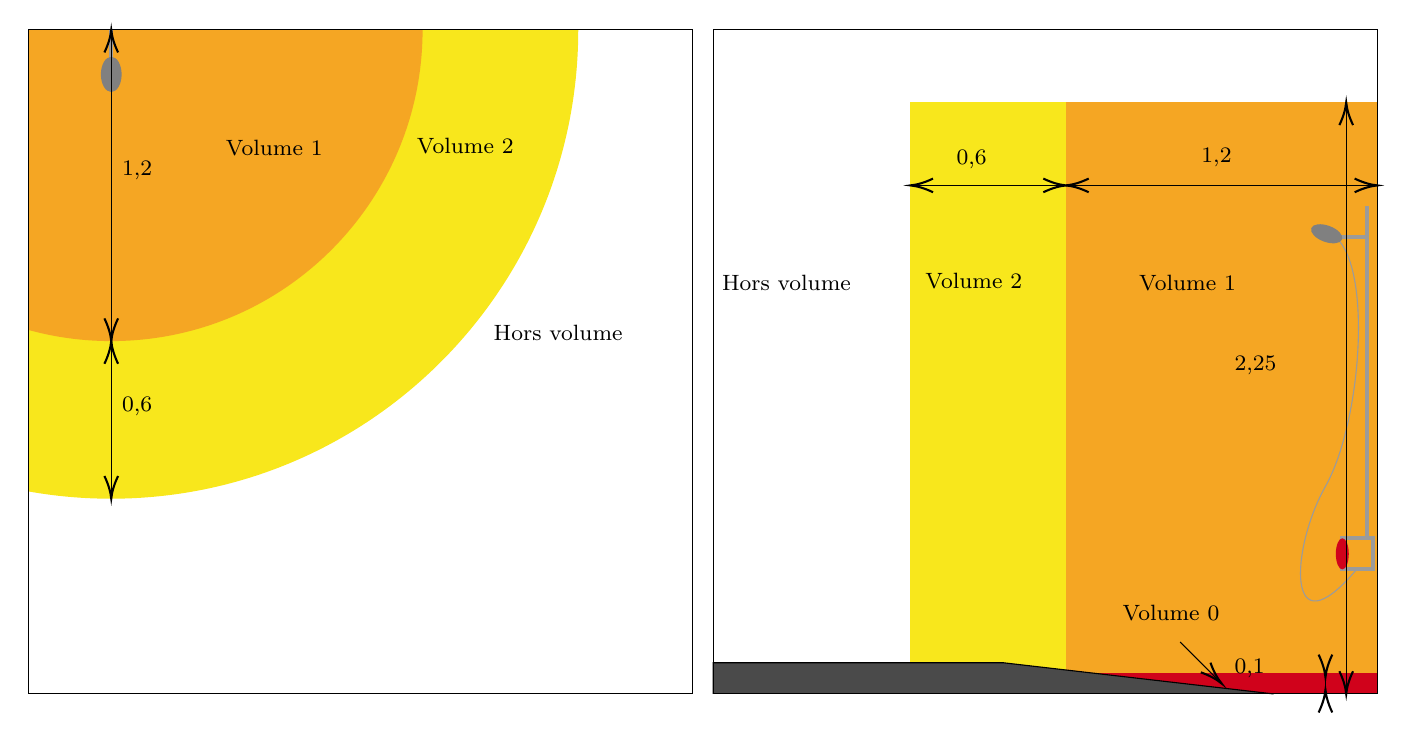
\begin{tikzpicture}[x=0.75pt,y=0.75pt,yscale=-1,xscale=1]
%uncomment if require: \path (0,550); %set diagram left start at 0, and has height of 550

%Shape: Rectangle [id:dp662524575372376] 
\draw  [draw opacity=0][fill={rgb, 255:red, 245; green, 166; blue, 35 }  ,fill opacity=1 ] (505,75) -- (655,75) -- (655,360) -- (505,360) -- cycle ;
%Shape: Path Data [id:dp8475067670718847] 
\draw  [draw opacity=0][fill={rgb, 255:red, 248; green, 231; blue, 28 }  ,fill opacity=1 ] (44.86,265.94) .. controls (31.26,265.94) and (17.94,264.73) .. (5,262.41) -- (5,40) -- (270,40) .. controls (270,164.78) and (169.2,265.94) .. (44.86,265.94) -- cycle ;
%Shape: Path Data [id:dp6391722198147811] 
\draw  [draw opacity=0][fill={rgb, 255:red, 245; green, 166; blue, 35 }  ,fill opacity=1 ] (45,190) .. controls (31.15,190) and (17.73,188.12) .. (5,184.61) -- (5,40) -- (195,40) .. controls (195,122.84) and (127.84,190) .. (45,190) -- cycle ;
%Straight Lines [id:da30342442827537275] 
\draw    (45,192) -- (45,263.94) ;
\draw [shift={(45,265.94)}, rotate = 270] [color={rgb, 255:red, 0; green, 0; blue, 0 }  ][line width=0.75]    (10.93,-3.29) .. controls (6.95,-1.4) and (3.31,-0.3) .. (0,0) .. controls (3.31,0.3) and (6.95,1.4) .. (10.93,3.29)   ;
\draw [shift={(45,190)}, rotate = 90] [color={rgb, 255:red, 0; green, 0; blue, 0 }  ][line width=0.75]    (10.93,-3.29) .. controls (6.95,-1.4) and (3.31,-0.3) .. (0,0) .. controls (3.31,0.3) and (6.95,1.4) .. (10.93,3.29)   ;
%Shape: Ellipse [id:dp9403307541201106] 
\draw  [draw opacity=0][fill={rgb, 255:red, 128; green, 128; blue, 128 }  ,fill opacity=1 ] (40,61.5) .. controls (40,56.81) and (42.24,53) .. (45,53) .. controls (47.76,53) and (50,56.81) .. (50,61.5) .. controls (50,66.19) and (47.76,70) .. (45,70) .. controls (42.24,70) and (40,66.19) .. (40,61.5) -- cycle ;
%Straight Lines [id:da02087532483936594] 
\draw [color={rgb, 255:red, 155; green, 155; blue, 155 }  ,draw opacity=1 ][line width=1.5]    (635,140) -- (650,140) -- (650,125) -- (650,285) ;
%Shape: Rectangle [id:dp8026516698473696] 
\draw  [color={rgb, 255:red, 155; green, 155; blue, 155 }  ,draw opacity=1 ][line width=1.5]  (638,285) -- (653,285) -- (653,300) -- (638,300) -- cycle ;
%Shape: Ellipse [id:dp5617322251469574] 
\draw  [draw opacity=0][fill={rgb, 255:red, 208; green, 2; blue, 27 }  ,fill opacity=1 ] (635,292.5) .. controls (635,288.36) and (636.4,285) .. (638.12,285) .. controls (639.84,285) and (641.24,288.36) .. (641.24,292.5) .. controls (641.24,296.64) and (639.84,300) .. (638.12,300) .. controls (636.4,300) and (635,296.64) .. (635,292.5) -- cycle ;
%Curve Lines [id:da34152496146470934] 
\draw [color={rgb, 255:red, 155; green, 155; blue, 155 }  ,draw opacity=1 ]   (645,300) .. controls (610.74,340.76) and (613,290.13) .. (630,260) .. controls (647,229.87) and (652.89,156) .. (635,140) ;
%Straight Lines [id:da3291709567122535] 
\draw    (507,115) -- (653,115) ;
\draw [shift={(655,115)}, rotate = 180] [color={rgb, 255:red, 0; green, 0; blue, 0 }  ][line width=0.75]    (10.93,-3.29) .. controls (6.95,-1.4) and (3.31,-0.3) .. (0,0) .. controls (3.31,0.3) and (6.95,1.4) .. (10.93,3.29)   ;
\draw [shift={(505,115)}, rotate = 0] [color={rgb, 255:red, 0; green, 0; blue, 0 }  ][line width=0.75]    (10.93,-3.29) .. controls (6.95,-1.4) and (3.31,-0.3) .. (0,0) .. controls (3.31,0.3) and (6.95,1.4) .. (10.93,3.29)   ;
%Shape: Rectangle [id:dp3771388764567015] 
\draw  [draw opacity=0][fill={rgb, 255:red, 248; green, 231; blue, 28 }  ,fill opacity=1 ] (430,75) -- (505,75) -- (505,360) -- (430,360) -- cycle ;
%Shape: Ellipse [id:dp2508485797626314] 
\draw  [draw opacity=0][fill={rgb, 255:red, 128; green, 128; blue, 128 }  ,fill opacity=1 ] (629.22,142.02) .. controls (625.12,140.53) and (622.4,137.65) .. (623.15,135.59) .. controls (623.9,133.54) and (627.83,133.08) .. (631.93,134.57) .. controls (636.03,136.06) and (638.75,138.94) .. (638,141) .. controls (637.25,143.06) and (633.32,143.52) .. (629.22,142.02) -- cycle ;
%Straight Lines [id:da7753899978688642] 
\draw    (432,115) -- (503,115) ;
\draw [shift={(505,115)}, rotate = 180] [color={rgb, 255:red, 0; green, 0; blue, 0 }  ][line width=0.75]    (10.93,-3.29) .. controls (6.95,-1.4) and (3.31,-0.3) .. (0,0) .. controls (3.31,0.3) and (6.95,1.4) .. (10.93,3.29)   ;
\draw [shift={(430,115)}, rotate = 0] [color={rgb, 255:red, 0; green, 0; blue, 0 }  ][line width=0.75]    (10.93,-3.29) .. controls (6.95,-1.4) and (3.31,-0.3) .. (0,0) .. controls (3.31,0.3) and (6.95,1.4) .. (10.93,3.29)   ;
%Shape: Rectangle [id:dp5616018693868235] 
\draw  [draw opacity=0][fill={rgb, 255:red, 208; green, 2; blue, 27 }  ,fill opacity=1 ] (505,350) -- (655,350) -- (655,360) -- (505,360) -- cycle ;
%Straight Lines [id:da23151913869668295] 
\draw [fill={rgb, 255:red, 74; green, 74; blue, 74 }  ,fill opacity=1 ]   (335,360) -- (335,345) -- (475,345) -- (605,360) ;
%Shape: Square [id:dp20615639222385096] 
\draw   (335,40) -- (655,40) -- (655,360) -- (335,360) -- cycle ;
%Straight Lines [id:da4535884422765213] 
\draw    (640,77) -- (640,358) ;
\draw [shift={(640,360)}, rotate = 270] [color={rgb, 255:red, 0; green, 0; blue, 0 }  ][line width=0.75]    (10.93,-3.29) .. controls (6.95,-1.4) and (3.31,-0.3) .. (0,0) .. controls (3.31,0.3) and (6.95,1.4) .. (10.93,3.29)   ;
\draw [shift={(640,75)}, rotate = 90] [color={rgb, 255:red, 0; green, 0; blue, 0 }  ][line width=0.75]    (10.93,-3.29) .. controls (6.95,-1.4) and (3.31,-0.3) .. (0,0) .. controls (3.31,0.3) and (6.95,1.4) .. (10.93,3.29)   ;
%Straight Lines [id:da07910479855322938] 
\draw    (630,352) -- (630,358) ;
\draw [shift={(630,358)}, rotate = 90] [color={rgb, 255:red, 0; green, 0; blue, 0 }  ][line width=0.75]    (10.93,-3.29) .. controls (6.95,-1.4) and (3.31,-0.3) .. (0,0) .. controls (3.31,0.3) and (6.95,1.4) .. (10.93,3.29)   ;
\draw [shift={(630,352)}, rotate = 270] [color={rgb, 255:red, 0; green, 0; blue, 0 }  ][line width=0.75]    (10.93,-3.29) .. controls (6.95,-1.4) and (3.31,-0.3) .. (0,0) .. controls (3.31,0.3) and (6.95,1.4) .. (10.93,3.29)   ;
%Straight Lines [id:da2835004459782169] 
\draw [color={rgb, 255:red, 155; green, 155; blue, 155 }  ,draw opacity=1 ][line width=1.5]    (45,40) -- (45,53) ;
%Straight Lines [id:da9119507330949469] 
\draw    (45,42) -- (45,188) ;
\draw [shift={(45,190)}, rotate = 270] [color={rgb, 255:red, 0; green, 0; blue, 0 }  ][line width=0.75]    (10.93,-3.29) .. controls (6.95,-1.4) and (3.31,-0.3) .. (0,0) .. controls (3.31,0.3) and (6.95,1.4) .. (10.93,3.29)   ;
\draw [shift={(45,40)}, rotate = 90] [color={rgb, 255:red, 0; green, 0; blue, 0 }  ][line width=0.75]    (10.93,-3.29) .. controls (6.95,-1.4) and (3.31,-0.3) .. (0,0) .. controls (3.31,0.3) and (6.95,1.4) .. (10.93,3.29)   ;
%Shape: Square [id:dp387542858738239] 
\draw   (5,40) -- (325,40) -- (325,360) -- (5,360) -- cycle ;
%Straight Lines [id:da9701869004128781] 
\draw    (560,335) -- (578.59,353.59) ;
\draw [shift={(580,355)}, rotate = 225] [color={rgb, 255:red, 0; green, 0; blue, 0 }  ][line width=0.75]    (10.93,-3.29) .. controls (6.95,-1.4) and (3.31,-0.3) .. (0,0) .. controls (3.31,0.3) and (6.95,1.4) .. (10.93,3.29)   ;

% Text Node
\draw (49,102) node [anchor=north west][inner sep=0.75pt]   [align=left] {\footnotesize{\SI{1,2}{\meter}}};
% Text Node
\draw (49,216) node [anchor=north west][inner sep=0.75pt]   [align=left] {\footnotesize{\SI{0,6}{\meter}}};
% Text Node
\draw (569,96) node [anchor=north west][inner sep=0.75pt]   [align=left] {\footnotesize{\SI{1,2}{\meter}}};
% Text Node
\draw (451,97) node [anchor=north west][inner sep=0.75pt]   [align=left] {\footnotesize{\SI{0,6}{\meter}}};
% Text Node
\draw (585,196) node [anchor=north west][inner sep=0.75pt]   [align=left] {\footnotesize{\SI{2,25}{\meter}}};
% Text Node
\draw (585,342) node [anchor=north west][inner sep=0.75pt]   [align=left] {\footnotesize{\SI{0,1}{\meter}}};
% Text Node
\draw (436,156) node [anchor=north west][inner sep=0.75pt]   [align=left] {\footnotesize{Volume 2}};
% Text Node
\draw (539,157) node [anchor=north west][inner sep=0.75pt]   [align=left] {\footnotesize{Volume 1}};
% Text Node
\draw (191,91) node [anchor=north west][inner sep=0.75pt]   [align=left] {{\footnotesize Volume 2}};
% Text Node
\draw (99,92) node [anchor=north west][inner sep=0.75pt]   [align=left] {{\footnotesize Volume 1}};
% Text Node
\draw (338,157) node [anchor=north west][inner sep=0.75pt]   [align=left] {{\footnotesize Hors volume}};
% Text Node
\draw (228,181) node [anchor=north west][inner sep=0.75pt]   [align=left] {{\footnotesize Hors volume}};
% Text Node
\draw (531,316) node [anchor=north west][inner sep=0.75pt]   [align=left] {{\footnotesize Volume 0}};

\end{tikzpicture}
\end{figure}




%\end{document}



%--------------------------------------
%ELECTROTECHNIQUE - SCHEMA DE LIAISON A LA TERRE
%--------------------------------------

%utiliser les environnement \begin{comment} \end{comment} pour mettre en commentaire le préambule une fois la programmation appelée dans le document maître (!ne pas oublier de mettre en commentaire \end{document}!)

\begin{comment}

\documentclass[a4paper, 11pt, twoside, fleqn]{memoir}

\usepackage{AOCDTF}

\marqueurchapitre

%lien d'édition des figures Tikz sur le site mathcha.io (rajouter le lien d'une modification effectuée sur la figure tikz avec le nom du modificateur car il n'y a qu'un lien par compte)

%lien éditeur Bruno Douchy : https://www.mathcha.io/editor/4zmjBS4GfLpHL48e8frKpd9lfP0E5lDHXe51Ln

%--------------------------------------
%corps du document
%--------------------------------------

\begin{document} %corps du document
	\openleft %début de chapitre à gauche

\end{comment}

\begin{figure}
\caption{Répartition des volumes dans une salle d'eau avec baignoire}


\tikzset{every picture/.style={line width=0.5pt}} %set default line width to 0.75pt        

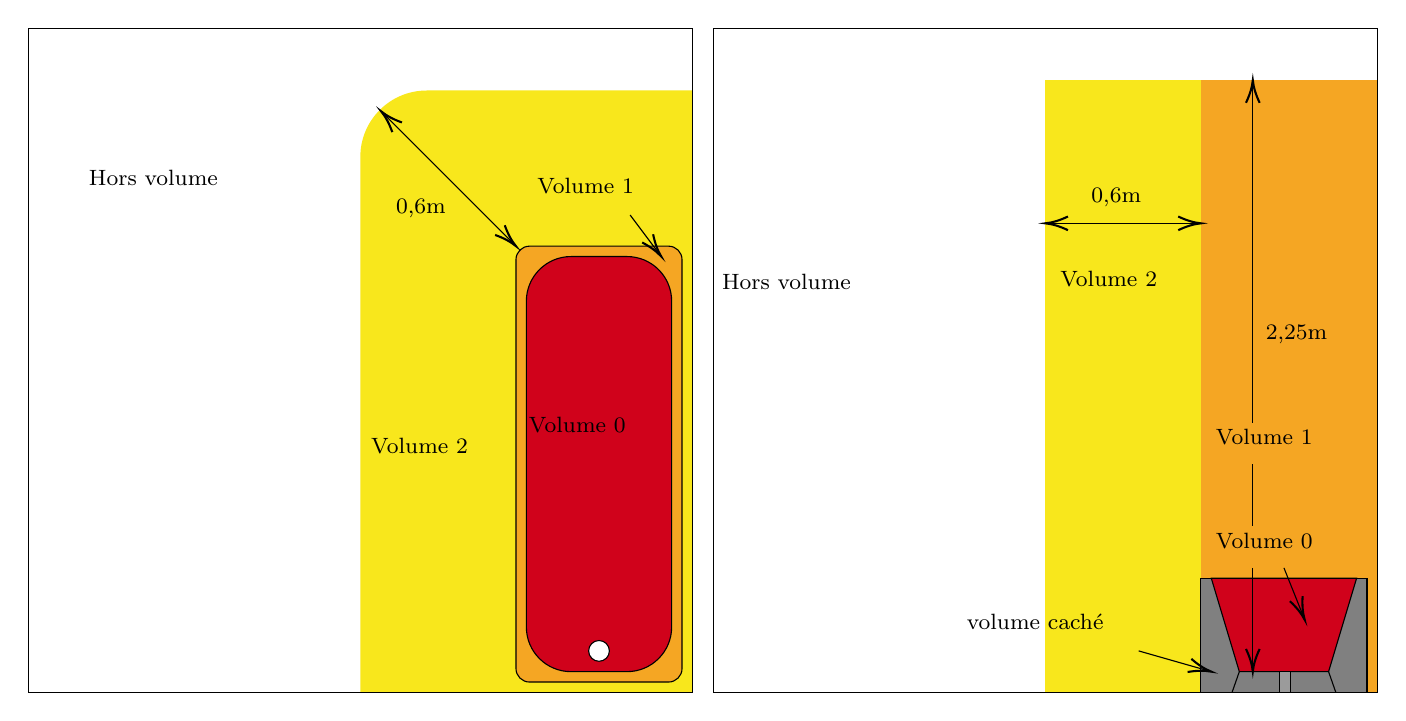
\begin{tikzpicture}[x=0.75pt,y=0.75pt,yscale=-1,xscale=1]
%uncomment if require: \path (0,550); %set diagram left start at 0, and has height of 550

%Shape: Rectangle [id:dp537465530048803] 
\draw  [draw opacity=0][fill={rgb, 255:red, 245; green, 166; blue, 35 }  ,fill opacity=1 ] (570,65) -- (655,65) -- (655,360) -- (570,360) -- cycle ;
%Rounded Single Corner Rect [id:dp9873012745251137] 
\draw  [draw opacity=0][fill={rgb, 255:red, 248; green, 231; blue, 28 }  ,fill opacity=1 ] (165,102) .. controls (165,84.33) and (179.33,70) .. (197,70) -- (325,70) -- (325,360) -- (165,360) -- cycle ;
%Rounded Rect [id:dp11224704269677876] 
\draw  [fill={rgb, 255:red, 245; green, 166; blue, 35 }  ,fill opacity=1 ] (240,151.5) .. controls (240,147.91) and (242.91,145) .. (246.5,145) -- (313.5,145) .. controls (317.09,145) and (320,147.91) .. (320,151.5) -- (320,348.5) .. controls (320,352.09) and (317.09,355) .. (313.5,355) -- (246.5,355) .. controls (242.91,355) and (240,352.09) .. (240,348.5) -- cycle ;
%Shape: Rectangle [id:dp6813821922304953] 
\draw  [draw opacity=0][fill={rgb, 255:red, 248; green, 231; blue, 28 }  ,fill opacity=1 ] (495,65) -- (570,65) -- (570,360) -- (495,360) -- cycle ;
%Straight Lines [id:da9776864357431949] 
\draw    (176.41,81.41) -- (238.59,143.59) ;
\draw [shift={(240,145)}, rotate = 225] [color={rgb, 255:red, 0; green, 0; blue, 0 }  ][line width=0.75]    (10.93,-3.29) .. controls (6.95,-1.4) and (3.31,-0.3) .. (0,0) .. controls (3.31,0.3) and (6.95,1.4) .. (10.93,3.29)   ;
\draw [shift={(175,80)}, rotate = 45] [color={rgb, 255:red, 0; green, 0; blue, 0 }  ][line width=0.75]    (10.93,-3.29) .. controls (6.95,-1.4) and (3.31,-0.3) .. (0,0) .. controls (3.31,0.3) and (6.95,1.4) .. (10.93,3.29)   ;
%Shape: Square [id:dp41030709608176064] 
\draw   (335,40) -- (655,40) -- (655,360) -- (335,360) -- cycle ;
%Shape: Square [id:dp14415595503059908] 
\draw   (5,40) -- (325,40) -- (325,360) -- (5,360) -- cycle ;
%Straight Lines [id:da04424757259652501] 
\draw    (295,130) -- (308.8,148.4) ;
\draw [shift={(310,150)}, rotate = 233.13] [color={rgb, 255:red, 0; green, 0; blue, 0 }  ][line width=0.75]    (10.93,-3.29) .. controls (6.95,-1.4) and (3.31,-0.3) .. (0,0) .. controls (3.31,0.3) and (6.95,1.4) .. (10.93,3.29)   ;
%Rounded Rect [id:dp9600049756918252] 
\draw  [fill={rgb, 255:red, 208; green, 2; blue, 27 }  ,fill opacity=1 ] (245,171.5) .. controls (245,159.63) and (254.63,150) .. (266.5,150) -- (293.5,150) .. controls (305.37,150) and (315,159.63) .. (315,171.5) -- (315,328.5) .. controls (315,340.37) and (305.37,350) .. (293.5,350) -- (266.5,350) .. controls (254.63,350) and (245,340.37) .. (245,328.5) -- cycle ;
%Shape: Circle [id:dp7093382716801047] 
\draw  [fill={rgb, 255:red, 255; green, 255; blue, 255 }  ,fill opacity=1 ] (275,340) .. controls (275,337.24) and (277.24,335) .. (280,335) .. controls (282.76,335) and (285,337.24) .. (285,340) .. controls (285,342.76) and (282.76,345) .. (280,345) .. controls (277.24,345) and (275,342.76) .. (275,340) -- cycle ;
%Shape: Rectangle [id:dp46214446507827656] 
\draw  [fill={rgb, 255:red, 128; green, 128; blue, 128 }  ,fill opacity=1 ] (570,305) -- (650,305) -- (650,360) -- (570,360) -- cycle ;
%Shape: Trapezoid [id:dp945587283320089] 
\draw  [fill={rgb, 255:red, 208; green, 2; blue, 27 }  ,fill opacity=1 ] (575,305) -- (588.5,350) -- (631.5,350) -- (645,305) -- cycle ;
%Straight Lines [id:da45767444398518653] 
\draw    (588.5,350) -- (585,360) ;
%Straight Lines [id:da303792904954273] 
\draw    (631.5,350) -- (635,360) ;
%Shape: Rectangle [id:dp35718485744867867] 
\draw  [fill={rgb, 255:red, 155; green, 155; blue, 155 }  ,fill opacity=1 ] (608,350) -- (613,350) -- (613,360) -- (608,360) -- cycle ;

%Straight Lines [id:da2781237207088538] 
\draw    (497,134) -- (568,134) ;
\draw [shift={(570,134)}, rotate = 180] [color={rgb, 255:red, 0; green, 0; blue, 0 }  ][line width=0.75]    (10.93,-3.29) .. controls (6.95,-1.4) and (3.31,-0.3) .. (0,0) .. controls (3.31,0.3) and (6.95,1.4) .. (10.93,3.29)   ;
\draw [shift={(495,134)}, rotate = 0] [color={rgb, 255:red, 0; green, 0; blue, 0 }  ][line width=0.75]    (10.93,-3.29) .. controls (6.95,-1.4) and (3.31,-0.3) .. (0,0) .. controls (3.31,0.3) and (6.95,1.4) .. (10.93,3.29)   ;
%Straight Lines [id:da9991563401347446] 
\draw    (595,300) -- (595,348) ;
\draw [shift={(595,350)}, rotate = 270] [color={rgb, 255:red, 0; green, 0; blue, 0 }  ][line width=0.75]    (10.93,-3.29) .. controls (6.95,-1.4) and (3.31,-0.3) .. (0,0) .. controls (3.31,0.3) and (6.95,1.4) .. (10.93,3.29)   ;
%Straight Lines [id:da9518092424958232] 
\draw    (595,67) -- (595,230) ;
\draw [shift={(595,65)}, rotate = 90] [color={rgb, 255:red, 0; green, 0; blue, 0 }  ][line width=0.75]    (10.93,-3.29) .. controls (6.95,-1.4) and (3.31,-0.3) .. (0,0) .. controls (3.31,0.3) and (6.95,1.4) .. (10.93,3.29)   ;
%Straight Lines [id:da21574516652189846] 
\draw    (595,250) -- (595,280) ;
%Straight Lines [id:da7442389799673409] 
\draw    (610,300) -- (619.26,323.14) ;
\draw [shift={(620,325)}, rotate = 248.2] [color={rgb, 255:red, 0; green, 0; blue, 0 }  ][line width=0.75]    (10.93,-3.29) .. controls (6.95,-1.4) and (3.31,-0.3) .. (0,0) .. controls (3.31,0.3) and (6.95,1.4) .. (10.93,3.29)   ;
%Straight Lines [id:da6922315454679567] 
\draw    (540,340) -- (573.08,349.45) ;
\draw [shift={(575,350)}, rotate = 195.95] [color={rgb, 255:red, 0; green, 0; blue, 0 }  ][line width=0.75]    (10.93,-3.29) .. controls (6.95,-1.4) and (3.31,-0.3) .. (0,0) .. controls (3.31,0.3) and (6.95,1.4) .. (10.93,3.29)   ;

% Text Node
\draw (501,156) node [anchor=north west][inner sep=0.75pt]   [align=left] {\footnotesize{Volume 2}};
% Text Node
\draw (576,232) node [anchor=north west][inner sep=0.75pt]   [align=left] {\footnotesize{Volume 1}};
% Text Node
\draw (169,236) node [anchor=north west][inner sep=0.75pt]   [align=left] {\footnotesize{Volume 2}};
% Text Node
\draw (249,111) node [anchor=north west][inner sep=0.75pt]   [align=left] {\footnotesize{Volume 1}};
% Text Node
\draw (338,157) node [anchor=north west][inner sep=0.75pt]   [align=left] {\footnotesize{Hors volume}};
% Text Node
\draw (33,107) node [anchor=north west][inner sep=0.75pt]   [align=left] {\footnotesize{Hors volume}};
% Text Node
\draw (245,226) node [anchor=north west][inner sep=0.75pt]   [align=left] {\footnotesize{Volume 0}};
% Text Node
\draw (181,121) node [anchor=north west][inner sep=0.75pt]   [align=left] {\footnotesize{0,6m}};
% Text Node
\draw (576,282) node [anchor=north west][inner sep=0.75pt]   [align=left] {\footnotesize{Volume 0}};
% Text Node
\draw (516,116) node [anchor=north west][inner sep=0.75pt]   [align=left] {\footnotesize{0,6m}};
% Text Node
\draw (600,182) node [anchor=north west][inner sep=0.75pt]   [align=left] {\footnotesize{2,25m}};
% Text Node
\draw (456,321) node [anchor=north west][inner sep=0.75pt]   [align=left] {\footnotesize{volume caché}};


\end{tikzpicture}

\end{figure}




%\end{document}



\begin{table}[t]
\caption{Caractéristiques des équipements électriques selon les volumes des salles d'eau}
\begin{threeparttable} %note dans tableau
\begin{tabularx}{\linewidth}{X ccccc}
\toprule
\makecell[C]{\multirow[c]{2}{*}{\thead{Appareils}}} 	& \multirow[c]{2}{*}{\thead{Mesure de\\protection}}		& \thead{Volume 0}		& \thead{Volume 1}		& \thead{Volume 2}		& \multirow{2}{*}{\thead{Hors volume}} \\
&&	IPX7		& IPX4\tnote{1}			& IPX4\tnote{1}			& \\
\midrule
\multicolumn{6}{l}{\textit{Lave-linge, sèche-linge}} \\
\middashrule			
& classe I													& interdit						& interdit 						& interdit						& autorisé \\
\addlinespace
\multicolumn{6}{l}{\textit{Appareils de chauffage}} \\
\middashrule
 				& classe I												& interdit						& interdit 						& interdit						& autorisé \\
												&classe II												& interdit						& interdit 						& autorisé						& autorisé \\
\addlinespace
\multicolumn{6}{l}{\textit{\'Eclairage}} \\
\middashrule
									& classe I													& interdit						& interdit 						& interdit						& autorisé \\
												& classe II													& interdit						& interdit 						& autorisé						& autorisé \\
												& \adjustbox{valign=t}{\makecell[{{p{2,5cm}}}]{TBTS (\SI{12}{\volt} $\mathdirectcurrent$ ou \SI{30}{\volt} $\sim$)}}												& autorisé\tnote{2}						& autorisé\tnote{2} 						& autorisé\tnote{2}						& autorisé\tnote{3} \\
\addlinespace
\multicolumn{6}{l}{\textit{Chauffe-eau instantané}}\\
\middashrule
				& classe I													& interdit						& autorisé\tnote{4} 					& autorisé\tnote{4}						& autorisé \\
\addlinespace
\multicolumn{6}{l}{\textit{Chauffe-eau à accumulation}} \\
\middashrule
				& classe I												& interdit						& autorisé\tnote{5} 					& autorisé\tnote{4}						& autorisé \\
\addlinespace
\multicolumn{6}{l}{\textit{Interrupteur}}\\
\middashrule
								& 																& interdit						& interdit 						& interdit						& autorisé \\
												& \adjustbox{valign=t}{\makecell[{{p{2,5cm}}}]{TBTS (\SI{12}{\volt} $\mathdirectcurrent$ ou \SI{30}{\volt} $\sim$)}}	& interdit						& autorisé\tnote{2} 						& autorisé\tnote{2}						& autorisé\tnote{3} \\
\addlinespace
\multicolumn{6}{l}{\textit{Prise de courant avec terre}}\\
\middashrule
			& 																& interdit						& interdit 						& interdit						& autorisé \\
\addlinespace
\multicolumn{6}{l}{\textit{Prise rasoir (\SIrange{10}{50}{\watt})}} \\
\middashrule
								& \adjustbox{valign=t}{\makecell[{{p{2,5cm}}}]{transformateur de séparation}}															& interdit						& interdit 						& autorisé						& autorisé \\
\addlinespace
\multicolumn{6}{l}{\textit{Transformateur de séparation}} \\
\middashrule
							& 															& interdit						& interdit 						& interdit						& autorisé \\
\addlinespace
\multicolumn{6}{l}{Canalisation} \\
\middashrule
							& 															& interdit						& autorisé\tnote{6} 						& autorisé\tnote{6}						& autorisé \\
\addlinespace
\multicolumn{6}{l}{\textit{Boitier de connexion}} \\
\middashrule
							& 															& interdit						& interdit\tnote{7} 						& interdit						& autorisé \\
\bottomrule
\end{tabularx}
\begin{tablenotes}
    \item[1] IP X5 si le volume est soumis à des jets d'eau pour des raisons de nettoyage (piscines, bains publics\ldots)\,;
    \item[2] Le transformateur de séparation doit être installé en dehors des volumes 1, 2 et 3\,;
	\item[3] La tension peut être portée à \SI{230}{\volt}\,;
	\item[4] Si l'appareil est alimenté directement sans boite de connexion\,;
	\item[5] Chauffe-eau horizontal installé le plus haut possible\,;
	\item[6] Limité à l'alimentation des appareils autorisés dans ces volumes\,;
	\item[7] Pour l'alimentation en direct d'un appareil et avec le respect de l'IP exigée par le volume ou elle se situe.
\end{tablenotes}
\end{threeparttable} %note dans tableau
\end{table}


\end{document}
